% \RequirePackage[2019/11/18]{latexrelease}
%% This is file `elsarticle-template-1a-num.tex',
%DIF LATEXDIFF DIFFERENCE FILE
%DIF DEL ..\PostThesis_Drafts\DC_SurveyDesign_Draft3_July2021.tex   Thu May  5 10:06:35 2022
%DIF ADD .\DC_SurveyDesign_PostSubmissionRevisions.tex              Tue Dec 27 14:32:32 2022
%%
%% Copyright 2009 Elsevier Ltd
%%
%% This file is part of the 'Elsarticle Bundle'.
%% ---------------------------------------------
%%
%% It may be distributed under the conditions of the LaTeX Project Public
%% License, either version 1.2 of this license or (at your option) any
%% later version.  The latest version of this license is in
%%    http://www.latex-project.org/lppl.txt
%% and version 1.2 or later is part of all distributions of LaTeX
%% version 1999/12/01 or later.
%%
%% The list of all files belonging to the 'Elsarticle Bundle' is
%% given in the file `manifest.txt'.
%%
%% Template article for Elsevier's document class `elsarticle'
%% with numbered style bibliographic references
%%
%% $Id: elsarticle-template-1a-num.tex 151 2009-10-08 05:18:25Z rishi $
%% $URL: http://lenova.river-valley.com/svn/elsbst/trunk/elsarticle-template-1a-num.tex $
%%
% \documentclass[preprint,12pt]{elsarticle}
\documentclass[preprint,authoryear,12pt]{elsarticle}
\usepackage{geometry}
\usepackage{afterpage}
\geometry{letterpaper, left=1.25in, right=1.25in, top=1.0in, bottom=1.0in}

%% Use the option review to obtain double line spacing
%% \documentclass[preprint,review,12pt]{elsarticle}

%% Use the options 1p,twocolumn; 3p; 3p,twocolumn; 5p; or 5p,twocolumn
%% for a journal layout:
%% \documentclass[final,1p,times]{elsarticle}
% \documentclass[final,1p,times,twocolumn]{elsarticle}
%% \documentclass[final,3p,times]{elsarticle}
%% \documentclass[final,3p,times,twocolumn]{elsarticle}
%% \documentclass[final,5p,times]{elsarticle}

% \documentclass[final,authoryear,5p,times,twocolumn]{elsarticle}

%% if you use PostScript figures in your article
%% use the graphics package for simple commands
%% \usepackage{graphics}
%% or use the graphicx package for more complicated commands
%% \usepackage{graphicx}
%% or use the epsfig package if you prefer to use the old commands
%% \usepackage{epsfig}

%% The amssymb package provides various useful mathematical symbols
\usepackage{amssymb}
%% The amsthm package provides extended theorem environments
%% \usepackage{amsthm}

%% The lineno packages adds line numbers. Start line numbering with
%% \begin{linenumbers}, end it with \end{linenumbers}. Or switch it on
%% for the whole article with \linenumbers after \end{frontmatter}.
\usepackage{lineno}

%% natbib.sty is loaded by default. However, natbib options can be
%% provided with \biboptions{...} command. Following options are
%% valid:

%%   round  -  round parentheses are used (default)
%%   square -  square brackets are used   [option]
%%   curly  -  curly braces are used      {option}
%%   angle  -  angle brackets are used    <option>
%%   semicolon  -  multiple citations separated by semi-colon
%%   colon  - same as semicolon, an earlier confusion
%%   comma  -  separated by comma
%%   numbers-  selects numerical citations
%%   super  -  numerical citations as superscripts
%%   sort   -  sorts multiple citations according to order in ref. list
%%   sort&compress   -  like sort, but also compresses numerical citations
%%   compress - compresses without sorting
%%
%% \biboptions{comma,round}

% \biboptions{}
\usepackage{hyperref}
% \usepackage{numcompress}

% \makeatletter
% \providecommand{\doi}[1]{%
%   \begingroup
%     \let\bibinfo\@secondoftwo
%     \urlstyle{rm}%
%     \href{http://dx.doi.org/#1}{%
%       doi:\discretionary{}{}{}%
%       \nolinkurl{#1}%
%     }%
%   \endgroup
% }
% \makeatother

\usepackage[T1]{fontenc}
\usepackage[utf8]{inputenc} % The default since 2018
\usepackage{amsmath}
% \usepackage{breqn}
% \ExplSyntaxOn
% \cs_set_eq:NN \intexpr_eval:w \int_eval:w
% \cs_set_eq:NN \intexpr_eval_end: \int_eval_end:
% \ExplSyntaxOff

% \usepackage{array, makecell}
% \usepackage{makecell}

\newcommand{\midtilde}{\raisebox{-0.25\baselineskip}{\textasciitilde}}
\newcommand{\IcelandicDh}{\textnormal{ð}}
%DIF 109a109
% \newcommand{\midtilde}{\raisebox{-0.5\baselineskip}{\Large{\textasciitilde}}} %DIF > 
%DIF -------

\usepackage{color}
\usepackage{color, colortbl}
\definecolor{greytext}{gray}{0.5}

\usepackage{enumitem}
\usepackage{boldline}


\usepackage{subcaption}
\usepackage{changepage}
\usepackage{rotating}
\usepackage{lscape}
%DIF 122a123-125
 %DIF > 
\usepackage{booktabs} %DIF > 
\usepackage{array} %DIF > 
%DIF -------
% \usepackage{pdflscape}
% \usepackage{afterpage}


\journal{Journal of Applied Geophysics}
%DIF PREAMBLE EXTENSION ADDED BY LATEXDIFF
%DIF UNDERLINE PREAMBLE %DIF PREAMBLE
\RequirePackage[normalem]{ulem} %DIF PREAMBLE
\RequirePackage{color}\definecolor{RED}{rgb}{1,0,0}\definecolor{BLUE}{rgb}{0,0,1} %DIF PREAMBLE
\providecommand{\DIFaddtex}[1]{{\protect\color{blue}\uwave{#1}}} %DIF PREAMBLE
\providecommand{\DIFdeltex}[1]{{\protect\color{red}\sout{#1}}}                      %DIF PREAMBLE
%DIF SAFE PREAMBLE %DIF PREAMBLE
\providecommand{\DIFaddbegin}{} %DIF PREAMBLE
\providecommand{\DIFaddend}{} %DIF PREAMBLE
\providecommand{\DIFdelbegin}{} %DIF PREAMBLE
\providecommand{\DIFdelend}{} %DIF PREAMBLE
\providecommand{\DIFmodbegin}{} %DIF PREAMBLE
\providecommand{\DIFmodend}{} %DIF PREAMBLE
%DIF FLOATSAFE PREAMBLE %DIF PREAMBLE
\providecommand{\DIFaddFL}[1]{\DIFadd{#1}} %DIF PREAMBLE
\providecommand{\DIFdelFL}[1]{\DIFdel{#1}} %DIF PREAMBLE
\providecommand{\DIFaddbeginFL}{} %DIF PREAMBLE
\providecommand{\DIFaddendFL}{} %DIF PREAMBLE
\providecommand{\DIFdelbeginFL}{} %DIF PREAMBLE
\providecommand{\DIFdelendFL}{} %DIF PREAMBLE
%DIF HYPERREF PREAMBLE %DIF PREAMBLE
\providecommand{\DIFadd}[1]{\texorpdfstring{\DIFaddtex{#1}}{#1}} %DIF PREAMBLE
\providecommand{\DIFdel}[1]{\texorpdfstring{\DIFdeltex{#1}}{}} %DIF PREAMBLE
%DIF COLORLISTINGS PREAMBLE %DIF PREAMBLE
\RequirePackage{listings} %DIF PREAMBLE
\RequirePackage{color} %DIF PREAMBLE
\lstdefinelanguage{DIFcode}{ %DIF PREAMBLE
%DIF DIFCODE_UNDERLINE %DIF PREAMBLE
  moredelim=[il][\color{red}\sout]{\%DIF\ <\ }, %DIF PREAMBLE
  moredelim=[il][\color{blue}\uwave]{\%DIF\ >\ } %DIF PREAMBLE
} %DIF PREAMBLE
\lstdefinestyle{DIFverbatimstyle}{ %DIF PREAMBLE
    language=DIFcode, %DIF PREAMBLE
    basicstyle=\ttfamily, %DIF PREAMBLE
    columns=fullflexible, %DIF PREAMBLE
    keepspaces=true %DIF PREAMBLE
} %DIF PREAMBLE
\lstnewenvironment{DIFverbatim}{\lstset{style=DIFverbatimstyle}}{} %DIF PREAMBLE
\lstnewenvironment{DIFverbatim*}{\lstset{style=DIFverbatimstyle,showspaces=true}}{} %DIF PREAMBLE
%DIF END PREAMBLE EXTENSION ADDED BY LATEXDIFF

\begin{document}

\begin{frontmatter}

\title{Using DC Resistivity Ring Array Surveys to Resolve Conductive Structures Around Tunnels or Mine-Workings}
%DIF >  \title{Using a DC Resistivity Survey Comprised of an Ensemble of Ring Arrays to Resolve Conductive Structures Around Tunnels or Mine-Workings}

%% use optional labels to link authors explicitly to addresses:
%% \author[label1,label2]{<author name>}
%% \address[label1]{<address>}
%% \address[label2]{<address>}

\author[1,2]{Michael A. Mitchell\corref{mycorrespondingauthor}}
\cortext[mycorrespondingauthor]{Corresponding author}
\ead{mamitchell@usgs.gov}

\author[1]{Douglas W. Oldenburg}

\address[1]{Geophysical Inversion Facility (GIF), \\
Department of Earth, Ocean and Atmospheric Sciences, \\
University of British Columbia, \\
2020-2207 Main Mall, \\
Vancouver, British Columbia \\
Canada, V6T 1Z4}

\DIFdelbegin %DIFDELCMD < \address[2]{California Volcano Observatory, \\
%DIFDELCMD < Volcano Science Center, \\
%DIFDELCMD < U.S. Geological Survey, \\
%DIFDELCMD < 345 Middlefield Rd., MS 910 \\
%DIFDELCMD < Menlo Park, CA 94025}
%DIFDELCMD < %%%
\DIFdelend \DIFaddbegin \address[2]{U.S. Geological Survey, \\
Volcano Science Center, \\
California Volcano Observatory, \\
350 N. Akron Rd., \\
Moffett Field, CA 94035}
\DIFaddend


\begin{abstract}
In underground environments, conventional \DIFdelbegin \DIFdel{DC }\DIFdelend \DIFaddbegin \DIFadd{direct current (DC) }\DIFaddend resistivity surveys with a single linear array of electrodes produce fundamentally non-unique inversions. These non-uniqueness and model resolution issues stem from limitations placed on the location of transmitters (TXs) and receivers (RXs) by the geometry of existing tunnels and boreholes. \DIFdelbegin \DIFdel{Poorly exciting or sampling }\DIFdelend \DIFaddbegin \DIFadd{Poor excitation and/or sampling of }\DIFaddend the region of interest (ROI) can create artifacts and reduce the resolution of the recovered model.

To address these problems we propose the use of \DIFdelbegin \DIFdel{ring arrays }\DIFdelend \DIFaddbegin \DIFadd{an ensemble of ring arrays, }\DIFaddend which are created by placing one or more electrodes in each face \DIFaddbegin \DIFadd{(sidewalls, floor, and ceiling) }\DIFaddend of the tunnel to form a ring of electrodes at each along-tunnel location. Using a series of increasingly complex synthetic models\DIFaddbegin \DIFadd{, }\DIFaddend we assess the benefits of ring arrays and show that they can be used to better constrain the location and shape of anomalous bodies around the tunnel.

Although ring arrays significantly improve the resolution of the recovered model, the size of the comprehensive ring array survey increases rapidly with the number of electrodes used. To balance model resolution and survey size\DIFaddbegin \DIFadd{, }\DIFaddend we developed a physics-based survey design methodology. In this methodology, TXs are selected based upon secondary charge accumulations on a test block that is moved through the ROI. Although this \DIFaddbegin \DIFadd{survey design methodology }\DIFaddend does not produce a strictly optimal survey\DIFdelbegin \DIFdel{design}\DIFdelend , it balances model resolution and survey size in a practical and computationally efficient manner.

Since the ring array more accurately estimates the around-tunnel location of targets and ensures that targets on all sides of the tunnel are detected, it is ideally suited to tunnel-based environments. Our results show that only about $6\%$ of the possible TXs and $0.5\%$ of the RXs in the comprehensive ring array survey are needed to retain the improvements in resolution. \DIFdelbegin \DIFdel{This allows }\DIFdelend \DIFaddbegin \DIFadd{Therefore, }\DIFaddend economical ring array surveys \DIFdelbegin \DIFdel{to }\DIFdelend \DIFaddbegin \DIFadd{can }\DIFaddend be designed for both reconnaissance and target characterization. Following the inversion of the reconnaissance dataset, additional rings can be added to reduce the inter-ring spacing or off-tunnel boreholes can be added to the region around identified anomalies to increase resolution as required.

%DIF <  Since ring arrays more accurately estimates the around-tunnel location of targets and ensure that targets on all sides of the tunnel are detected without greatly increasing the size of the survey, they are ideally suited to tunnel-based environments.
\DIFdelbegin %DIFDELCMD <

%DIFDELCMD < %%%
\DIFdelend \end{abstract}

\begin{keyword}
%% keywords here, in the form: keyword \sep keyword
DC \DIFdelbegin \DIFdel{resistivity }\DIFdelend \DIFaddbegin \DIFadd{Resistivity }\DIFaddend (ERT/ERI) \sep 3-D \DIFdelbegin \DIFdel{inversion }\DIFdelend \DIFaddbegin \DIFadd{Inversion }\DIFaddend \sep Survey Design \sep In-mine \sep Tunnel \DIFaddbegin \sep \DIFadd{SimPEG
}\DIFaddend

%% MSC codes here, in the form: \MSC code \sep code
%% or \MSC[2008] code \sep code (2000 is the default)

\end{keyword}

\end{frontmatter}

\noindent \textbf{CRediT authorship contribution statement} \\
\textbf{Michael A. Mitchell:} Conceptualization, Methodology, Formal analysis, Investigation, Writing-Original Draft, \DIFdelbegin \DIFdel{Writing - Review }\DIFdelend \DIFaddbegin \DIFadd{Writing-Review }\DIFaddend \& Editing, Funding Acquisition. \DIFaddbegin \\
\DIFaddend \textbf{Douglas W. Oldenburg:} Conceptualization, Methodology, Supervision, \DIFdelbegin \DIFdel{Writing - Review }\DIFdelend \DIFaddbegin \DIFadd{Writing-Review }\DIFaddend \& Editing, Funding Acquisition.

%%
%% Start line numbering here if you want
%%
\linenumbers

%% main text

\section{Introduction}
\label{Introduction}

\DIFdelbegin \DIFdel{DC }\DIFdelend \DIFaddbegin \DIFadd{Direct current (DC) }\DIFaddend resistivity surveys, which allow us to image variations in the electrical conductivity of the subsurface, can be used in any application where there is a conductivity contrast between the target and background. In a DC resistivity survey a constant current is injected between a pair of current or transmitter (TX) electrodes and potential differences are measured between one or more pairs of receiver (RX) electrodes. The accumulation of electrical charge on the interface between regions of differing electrical conductivities alters the measured potential differences. The observed \DIFdelbegin \DIFdel{variations the }\DIFdelend \DIFaddbegin \DIFadd{differences in }\DIFaddend measured potentials can be used to construct a model showing variations in the subsurface distribution of electrical conductivity using geophysical inversion. Some applications in which DC resistivity surveys are useful include: mapping aquifers, tracking environmental containments in groundwater,  mineral exploration, geothermal exploration and monitoring, and void detection in karst terrain.

Although DC resistivity surveys have been used extensively above ground since the 1950s, most studies involving subterranean use have occurred in the last 30 years. In one of the earliest applications, \cite{Scott1968} used \DIFdelbegin \DIFdel{1D }\DIFdelend \DIFaddbegin \DIFadd{one-dimensional (1-D) }\DIFaddend Wenner array soundings along the walls of a tunnel to characterize the competency of the rock and measure the thickness of fractured material from blasting. In-mine DC resistivity soundings and \DIFdelbegin \DIFdel{2D }\DIFdelend \DIFaddbegin \DIFadd{two-dimensional (2-D) }\DIFaddend arrays have been used in Germany to estimate the free water content and monitor wet regions within old salt mines which are being used for the storage of radioactive waste \citep{Kessels1985,Yaramanci2000}. For mineral exploration in Japan \cite{Sasaki1990} used a \DIFdelbegin \DIFdel{2D }\DIFdelend \DIFaddbegin \DIFadd{2-D }\DIFaddend ERT inversion of surface-to-tunnel and tunnel-to-tunnel DC resistivity data to map disseminated copper ore at a mine site and \cite{Arai1995} used a 2.5\DIFdelbegin \DIFdel{D }\DIFdelend \DIFaddbegin \DIFadd{-D }\DIFaddend ERT inversion to map the location of a resistive lead-zinc sulphide ore vein within a Japanese mine. \cite{Ramirez1996} showed that \DIFdelbegin \DIFdel{3D }\DIFdelend \DIFaddbegin \DIFadd{three-dimensional (3-D) }\DIFaddend ERT can be used to monitor underground storage tanks for leaks. In South Africa\DIFaddbegin \DIFadd{, }\DIFaddend researchers have used tunnel to tunnel ERT surveys to identify potholes, dykes, and iron-rich ultramafic pegmatite (IRUP) bodies that disrupt ore zones in platinum mines \citep{Schoor2005,VanSchoor2010}. To characterize and monitor small scale rock fracturing due to excavation\DIFaddbegin \DIFadd{, }\DIFaddend \cite{Kruschwitz2004} and \cite{Gibert2006} used \DIFdelbegin \DIFdel{2D }\DIFdelend \DIFaddbegin \DIFadd{2-D }\DIFaddend DC modeling and inversion of a few rings of electrodes placed around the circumference of a tunnel. In Chinese coal mines, a great deal of research has been undertaken to develop DC resistivity techniques to detect water-bearing structures ahead of the cutting machinery \citep{Wang2011,Han2011}.

Much of our current research builds upon work done by \DIFdelbegin \DIFdel{\mbox{%DIFAUXCMD
\cite{Maxwell2005,Eso2006,Eso2006a,Eso2006b,Cisyk2014,Maxwell2016} }\hskip0pt%DIFAUXCMD
and \mbox{%DIFAUXCMD
\cite{Mitchell2016,Mitchell2016a} }\hskip0pt%DIFAUXCMD
}\DIFdelend \DIFaddbegin \DIFadd{\mbox{%DIFAUXCMD
\cite{Maxwell2005}}\hskip0pt%DIFAUXCMD
, \mbox{%DIFAUXCMD
\cite{Eso2006a,Eso2006b,Eso2006}}\hskip0pt%DIFAUXCMD
, \mbox{%DIFAUXCMD
\cite{Cisyk2014}}\hskip0pt%DIFAUXCMD
, \mbox{%DIFAUXCMD
\cite{Maxwell2016} }\hskip0pt%DIFAUXCMD
and \mbox{%DIFAUXCMD
\cite{Mitchell2016a,Mitchell2016} }\hskip0pt%DIFAUXCMD
}\DIFaddend at the Mosaic potash mines near Esterhazy, Saskatchewan. Here they conducted several \DIFdelbegin \DIFdel{2D and 3D }\DIFdelend \DIFaddbegin \DIFadd{2-D and 3-D }\DIFaddend DC resistivity studies to map regions of wet salt and brine. To improve resolution in their \DIFdelbegin \DIFdel{3D surveys}\DIFdelend \DIFaddbegin \DIFadd{3-D surveys, }\DIFaddend off-plane electrodes were placed in raises, sub-drifts, and off-tunnel boreholes to better constrain the location of conductive targets. These studies, along with nearly all of the others listed above, discuss our inability to properly resolve \DIFdelbegin \DIFdel{3D structures with 2D }\DIFdelend \DIFaddbegin \DIFadd{3-D structures with 2-D }\DIFaddend arrays or a limited number of off-plane electrodes in \DIFdelbegin \DIFdel{3D surveys. This highlights }\DIFdelend \DIFaddbegin \DIFadd{3-D surveys. These challenges highlight }\DIFaddend the need for further research and refined survey design methodologies for in-mine or tunnel-based environments.

Underground environments, such as tunnels or mine-workings, \DIFdelbegin \DIFdel{are challenging environments in which to collect }\DIFdelend \DIFaddbegin \DIFadd{present challenges for }\DIFaddend DC resistivity data \DIFaddbegin \DIFadd{collection }\DIFaddend due to the limited electrode geometry afforded by the tunnels. Unlike surface applications\DIFaddbegin \DIFadd{, }\DIFaddend where a dense grid of transmitters (TXs) and receivers (RXs) can be deployed to maximize model resolution within the region of interest (ROI), the subterranean environment often limits the location of TXs and RXs to existing tunnels, boreholes, or other workings. \DIFdelbegin \DIFdel{This }\DIFdelend \DIFaddbegin \DIFadd{These physical limitations on the location of TXs and RXs }\DIFaddend can significantly reduce model resolution and create non-uniqueness issues when the target region is not properly sampled. \DIFaddbegin \DIFadd{\mbox{%DIFAUXCMD
\citet{Tsourlos2011} }\hskip0pt%DIFAUXCMD
noted similar challenges when using borehole-to-surface arrays.
}\DIFaddend

These limitations were highlighted \DIFdelbegin \DIFdel{while reading about }\DIFdelend \DIFaddbegin \DIFadd{by }\DIFaddend previous studies and \DIFdelbegin \DIFdel{working }\DIFdelend \DIFaddbegin \DIFadd{through work }\DIFaddend on two underground DC resistivity field datasets, one from the Mosaic K2 potash mine near Esterhazy, Saskatchewan \citep{Mitchell2016a,Mitchell2016}\DIFaddbegin \DIFadd{, }\DIFaddend and the other from the Laboratoire Souterrain \`a Bas Bruit (LSBB) in Rustrel, Vaucluse, France \citep{Maxwell2010}. To confidently interpret the inversion results\DIFaddbegin \DIFadd{, }\DIFaddend several questions needed to be addressed regarding the resolution of the recovered conductivity models. Two synthetic tunnel models, which mimicked the field examples, were created to investigate these questions. The first is a straight section of tunnel, akin to LSBB, while the second contains a tunnel laid out in an asymmetric horseshoe as in the Mosaic example. While working with these synthetic models the following pitfalls were observed.

When collecting DC data along a straight section of tunnel, conventional surveys used only a single linear array of electrodes placed along one face \DIFaddbegin \DIFadd{(sidewall, floor, or ceiling) }\DIFaddend of the tunnel. Although a \DIFdelbegin \DIFdel{2D }\DIFdelend \DIFaddbegin \DIFadd{2-D }\DIFaddend array of this type can often constrain the along-tunnel location of a potential target it cannot resolve the target's around-tunnel location and poorly constrains how far the target is away from the tunnel. Similar challenges arise with more complex tunnel geometries if most of the transmitters and receivers fall on or near the same depth plane. In this situation, it is difficult or impossible to determine where the anomalous bodies are located relative to the measurement plane.


%DIF <  Figures \ref{fig:ResolutionUniqueness_Intro_StraightTunnel_MultiBlk_Isosurfaces} and \ref{fig:ResolutionUniqueness_Intro_Horseshoe_SynthMosaic2_Isosurfaces} clearly illustrate these limitations of the single linear array. Figure \ref{fig:ResolutionUniqueness_Intro_StraightTunnel_MultiBlk_Isosurfaces} shows the inversion result from a comprehensive dipole-dipole dataset collected using a single linear array of electrodes running down the ceiling of a straight tunnel. Electrode locations are shown by the black dots placed a 5 m intervals along the tunnel ceiling. Although there are three conductive blocks in the synthetic model, whose shapes and locations are shown by the black outlines, the inversion model only recovers a single ring shaped conductive anomaly. The inversion correctly identified the along-tunnel location of the large block above the southern edge of the tunnel but has smeared the anomaly down around the sides of the tunnel. This illustrates the dataset's inability to constrain the location of the anomaly around the tunnel. The inversion fails to recover the other two conductive blocks at all. This is likely because of their further proximity from the electrodes, in the tunnel ceiling, and their smaller secondary responses relative to the upper block.
\DIFdelbegin %DIFDELCMD <

%DIFDELCMD < %%%
%DIF <  \begin{figure}[htp]{}
%DIF <  \captionsetup[subfigure]{labelformat=empty}
%DIF <     \begin{center}
%DIF <        \begin{subfigure}{0.45\linewidth}
%DIF <           \begin{picture}(100,0)
%DIF <              \put(53,0){\scriptsize{\textbf{West View}}}
%DIF <           \end{picture}
%DIF <        \end{subfigure}\hspace{-0.8cm}
%DIF <        \qquad
%DIF <        \begin{subfigure}{0.45\linewidth}
%DIF <           \begin{picture}(100,0)
%DIF <              \put(38,0){\scriptsize{\textbf{Top View}}}
%DIF <           \end{picture}
%DIF <        \end{subfigure}\hspace{-0.8cm}
%DIF <        \qquad
%DIF <        \vspace{0.1cm}
%DIFDELCMD <

%DIFDELCMD < %%%
%DIF <        \begin{subfigure}{0.55\linewidth}
%DIF <           % \label{fig:MultiBlk_StraightTunnel_SingleLinear_West}
%DIF <           \sbox0{\includegraphics[trim=0cm 0cm 0cm 0cm, clip=true,width=\linewidth]{./Figures/SingleLinearArray/MultiBlk_StraightTunnel_SingleLinear_Top_2ISO_Crop.png}}
%DIF <           \includegraphics[height=\ht0,keepaspectratio]{./Figures/SingleLinearArray/MultiBlk_StraightTunnel_SingleLinear_West_2ISO_noCB_Crop.png}
%DIF <        \end{subfigure}
%DIF <        \hspace{-4.0cm}
%DIF <        \qquad
%DIF <        \begin{subfigure}{0.55\linewidth}
%DIF <           % \label{fig:MultiBlk_StraightTunnel_SingleLinear_South}
%DIF <           \includegraphics[trim=0cm 0cm 0cm 0cm, clip=true,width=\linewidth]{./Figures/SingleLinearArray/MultiBlk_StraightTunnel_SingleLinear_Top_2ISO_Crop.png}
%DIF <        \end{subfigure}
%DIF <        \vspace{0.15cm}
%DIFDELCMD <

%DIFDELCMD < %%%
%DIF <     \end{center}
%DIF <  \vspace{-0.55cm}
%DIF <  \caption{West and top volumetric cutoff views of the inversion model from a comprehensive dipole-dipole dataset collected using a single linear array of electrodes running down the tunnel ceiling. This result shows how poorly the inversion recovers the three conductive targets within the synthetic multiple block model. The yellow and blue-green volumes show regions of high ($\geq$ 0.01 S/m) and intermediate ($\geq$ 0.007 S/m) conductivities respectively while the blue cells denote the tunnel. The black outlines show the true location of the conductive blocks and black dots mark electrode locations.}
%DIF <  \label{fig:ResolutionUniqueness_Intro_StraightTunnel_MultiBlk_Isosurfaces}
%DIF <  \end{figure}
%DIFDELCMD <

%DIFDELCMD < %%%
%DIF <  Figure \ref{fig:ResolutionUniqueness_Intro_Horseshoe_SynthMosaic2_Isosurfaces} shows a slightly more complex example with a horseshoe shaped tunnel to simulate the tunnel layout from the Mosaic field dataset \citep{Mitchell2016a,Mitchell2016}. The conductive body, marked by the black outline, is meant to mimic a water inflow structure (see Section \ref{sec:RingArray_Development_Horseshoe_Synth_GeologicalTarget} for more details). The inversion of the comprehensive dipole-dipole dataset collected using a single linear array of electrodes running along the interior wall of the horseshoe shaped tunnel also struggles to resolve this synthetic model. The most pronounced shortcoming of this inversion is its inability to constrain the $z$-location of the conductor. Even though the conductive structure lies above the tunnel, the recovered anomaly is centered on the measurement/tunnel plane and extends symmetrically upwards and downwards. This makes it impossible for us to determine where the target lies relative to the measurement plane.
%DIFDELCMD <

%DIFDELCMD < %%%
%DIF <  \begin{figure}[htp]{}
%DIF <  \captionsetup[subfigure]{labelformat=empty}
%DIF <     \begin{center}
%DIF <        \begin{subfigure}{0.43\linewidth}
%DIF <           \begin{picture}(100,0)
%DIF <              \put(63,0){\scriptsize{\textbf{South View}}}
%DIF <           \end{picture}
%DIF <        \end{subfigure}\hspace{-0.8cm}
%DIF <        \qquad
%DIF <        \begin{subfigure}{0.54\linewidth}
%DIF <           \begin{picture}(100,0)
%DIF <              \put(78,0){\scriptsize{\textbf{Top View}}}
%DIF <           \end{picture}
%DIF <        \end{subfigure}\hspace{-0.8cm}
%DIF <        \qquad
%DIF <        \vspace{0.1cm}
%DIF <        \begin{subfigure}{0.43\linewidth}
%DIF <           \includegraphics[trim=0cm 0cm 0cm 0cm, clip=true,width=\linewidth]{./Figures/SingleLinearArray/SynthMosaic2_Horseshoe_SLA_South_NoCB_Crop.png}
%DIF <        \end{subfigure}
%DIF <        \hspace{-0.7cm}
%DIF <        \qquad
%DIF <        \begin{subfigure}{0.54\linewidth}
%DIF <           \includegraphics[trim=0cm 0cm 0cm 0cm, clip=true,width=\linewidth]{./Figures/SingleLinearArray/SynthMosaic2_Horseshoe_SLA_Top_Crop.png}
%DIF <        \end{subfigure}
%DIF <        \vspace{0.2cm}
%DIFDELCMD <

%DIFDELCMD < %%%
%DIF <     \end{center}
%DIF <  \vspace{-0.4cm}
%DIF <  \caption{Volumetric cutoffs of the inversion models as seen from the south and from above which show how the single linear array based survey in the horseshoe shaped tunnel recovered the synthetic Mosaic model. In these plots, the yellow and blue-green volumes show regions of ($\geq$ 0.015 S/m) and intermediate ($\geq$ 0.01 S/m) conductivities, while the blue cells denote the horseshoe shaped tunnel. Note the recovered model's inability to constrain the location of the conductive anomaly relative to the measurement plane. The black outlines show the true location of the conductive structure and the black dots mark electrode locations.}
%DIF <  \label{fig:ResolutionUniqueness_Intro_Horseshoe_SynthMosaic2_Isosurfaces}
%DIF <  \end{figure}
%DIFDELCMD <

%DIFDELCMD < %%%
\DIFdelend \subsection{Paper Outline}
Before proceeding with our investigation of model resolution and non-uniqueness\DIFaddbegin \DIFadd{, }\DIFaddend we start with a brief overview of forward modeling and inversion (see Section \ref{sec:Background}). These numerical processes are fundamental to our analysis since they allow us to simulate data given a conductivity model and reconstruct a geologically reasonable estimate of the conductivity model that fits the recorded data. We then proceed to describe our research.

To design a survey which addresses the identified model resolution and non-uniqueness issues we first need to understand why they occur. In Section \ref{sec:Resolution_&_NonUniqueness} we analyze these shortcomings using a series of simple examples that illustrate the impact of data detectability and sensitivity on inversion results. To address these model resolution and non-uniqueness issues\DIFaddbegin \DIFadd{, }\DIFaddend we propose the use of \DIFaddbegin \DIFadd{an ensemble of }\DIFaddend ring-shaped arrays of electrodes. The ring array is created by placing one or more electrodes in each face \DIFaddbegin \DIFadd{(sidewalls, floor, and ceiling) }\DIFaddend of the tunnel to form a ring of electrodes at each along-tunnel location. Using a series of synthetic models, which increase in complexity, we assess the benefits of these design modifications in Section \ref{sec:RingArray_Development}.

Since the full ring array survey typically uses four times more electrodes than the single linear array, \DIFaddbegin \DIFadd{for a given along-tunnel electrode spacing, }\DIFaddend it contains many more possible measurements and can be costly to collect. This prompted us to develop a new survey design methodology (see Section \ref{sec:RingArray_SurveyDesign}). In this methodology, TXs are selected based on secondary charge accumulation on a target test block\DIFaddbegin \DIFadd{, }\DIFaddend which is moved through the ROI. This \DIFaddbegin \DIFadd{metric }\DIFaddend ensures that a subset of TXs which best excite the ROI is selected. RXs for each of the selected TXs are then pseudo-randomly selected from a subset of measurements that are sufficiently sensitive to one or more of the test block locations. We do not claim that this is a strictly optimal survey design but show it to be a practical and computationally efficient procedure that balances improvements in model resolution and survey size.


\section{Background Theory}
\label{sec:Background}


Forward modeling and inversion are important tools for solving geophysical problems. Forward modeling allows us to compute predicted data given a conductivity model and inversion is used to reconstruct an estimate of the conductivity model from our observed data. Forward modeling is an integral part of inversion since it is used to determine how well the recovered model fits the observed data. The model is iteratively updated until a geologically reasonable solution is found which adequately fits the observed data. All of the DC forward modeling and inversions presented in this paper were completed using the open-source python package SimPEG \citep{Cockett2015}.

In the forward problem a \DIFdelbegin \DIFdel{3D }\DIFdelend \DIFaddbegin \DIFadd{3-D }\DIFaddend finite volume discretization on a staggered mesh, in which $\sigma$ and $\phi$ are defined on cell centers, is used solve the following system of partial differential equations \citep{Haber2000, Pidlisecky2007, Cockett2015, Cockett2016}.

\begin{equation}
   \nabla\cdot\sigma\nabla \phi = I(\delta(r - r_{s^{+}}) - \delta(r - r_{s^{-}}))
  \label{eq:DC_Eq}
\end{equation}

\noindent \DIFdelbegin \DIFdel{Where }\DIFdelend \DIFaddbegin \DIFadd{where }\DIFaddend $\sigma$ is the electrical conductivity, $\phi$ is the electric potential, and $I(\delta(r - r_{s^{+}}) - \delta(r - r_{s^{-}}))$ is the galvanic source term, which is represented by the sum of Delta Dirac functions centered about the positive and negative source electrode locations $r_{s^{+}}$ and $r_{s^{-}}$ scaled by the injection current ($I$). An octree mesh, where the cell refinement is a function of the electrode locations and conductivity structures, was used to greatly reduce the number of model cells from that of a standard tensor mesh \citep{Haber2007,Haber2012}.

Since the inverse problem is typically very under-determined \DIFdelbegin \DIFdel{, }\DIFdelend (i.e.\DIFaddbegin \DIFadd{, }\DIFaddend there are far more model cells than data), we pose it as a regularized Tikhonov optimization problem. The inverse problem is solved by finding an estimate of the true model ($\widehat{m}$), which minimizes the model objective function ($\Phi_m$), while driving the data misfit ($\Phi_d$) to its target level ($\Phi_{d}^*$).  This minimization problem can be formalized in the following manner.

\begin{eqnarray}
  \label{eq:globphi}
  \min \Phi = \Phi_d+\beta\Phi_m \\
  \mbox{s. t. } \Phi_{d} \leq \Phi_{d}^* \nonumber
\end{eqnarray}

\noindent \DIFdelbegin \DIFdel{Where }\DIFdelend \DIFaddbegin \DIFadd{where }\DIFaddend $\beta$ is a regularization parameter that controls the relative importance of the model objective function ($\Phi_{m}$) and the data misfit ($\Phi_{d}$).

The data misfit ($\Phi_{d}$) provides a quantitative measure of the difference between predicted data ($\vec{d}^{pred}$), derived through numerical modeling, and the observed data ($\vec{d}^{obs}$). We defined $\Phi_{d}$ as follows.

\begin{equation}
  \Phi_d = \sum^{n}_{i=0}\left(\DIFdelbegin \DIFdel{\frac{d^{pred}_i-d^{obs}_i}{\xi_i}}\DIFdelend \DIFaddbegin \DIFadd{\frac{d^{pred}_i - d^{obs}_i}{\xi_i}}\DIFaddend \right)^2 = \left\|\mathbf{W}_{d}\left(\mathbf{d}^{pred} - \mathbf{d}^{obs}\right)\right\|_2^2
  \label{eq:Phi_d}
\end{equation}

\noindent \DIFdelbegin \DIFdel{Where }\DIFdelend \DIFaddbegin \DIFadd{where }\DIFaddend $\xi_{i}$ is the standard deviation of the $i$th datum. The data weighting matrix $\mathbf{W}_{d} = \text{diag}\left[1/\xi_{1}, \cdots, 1/\xi_{n}\right]$. Since the data uncertainties, which are cumulatively referred to as the noise model, are typically unknown\DIFaddbegin \DIFadd{, }\DIFaddend they must be estimated \citep{Oldenburg2005}.

To control the complexity of the recovered model, we used the following formulation for the model objective function ($\Phi_{m}$).

\begin{equation}
\label{eq:Phi_m}
  \Phi_m = \left\|\mathbf{W}_s(\mathbf{m} - \mathbf{m}_{ref})\right\|_2^2 + \sum^{3}_{i=1}\left\|\mathbf{W}_i\mathbf{m}\right\|_2^2
%DIF <  \Phi_m = \left\|\mathbf{W}_s(\mathbf{m}-\mathbf{m}_{ref})\right\|_2^2 + \underbrace{\left\|\mathbf{W}_{x}\mathbf{m}\right\|_2^2 + \left\|\mathbf{W}_{y}\mathbf{m}\right\|_2^2 + \left\|\mathbf{W}_{z}\mathbf{m}\right\|_2^2}_{\left\|\mathbf{W}_{xyz}\mathbf{m}\right\|_2^2}
\end{equation}

\noindent \DIFdelbegin \DIFdel{Where }\DIFdelend \DIFaddbegin \DIFadd{where }\DIFaddend the first term controls the ``smallness'' of the model (i.e.\DIFaddbegin \DIFadd{, }\DIFaddend how close the current model ($\mathbf{m}$) is to the reference model ($\mathbf{m}_{ref}$)) and the summation contains directional derivative terms\DIFaddbegin \DIFadd{, }\DIFaddend which control the smoothness of the model in each direction. $\mathbf{W}_s$ is a diagonal matrix containing cell weights while the three components of $\mathbf{W}_i$ ($\mathbf{W}_x$, $\mathbf{W}_y$, and $\mathbf{W}_z$) combine finite difference operators and face weight vectors in each direction \citep{Oldenburg2005}.

More details regarding our formulation of the forward and inverse problem can be found in \citet{Mitchell2016a} and \citet{Mitchell2020}. For additional information on geophysical inversion\DIFaddbegin \DIFadd{, }\DIFaddend we refer the reader to the following\DIFdelbegin \DIFdel{books}\DIFdelend : \citet{Menke1984}, \citet{Parker1994}, \citet{Aster2012}, and \citet{Haber2014}. \citet{Oldenburg2005} \DIFdelbegin \DIFdel{provide }\DIFdelend \DIFaddbegin \DIFadd{provided }\DIFaddend a general overview of geophysical inversion in their tutorial while \citet{Li1994}, \citet{LaBrecque1996}, \citet{Loke1996}, \citet{Ramirez1996}, and \citet{Loke2013} are a few of the many papers which specifically discuss the inversion of DC resistivity data.


\section{Non-Uniqueness and Model Resolution in Tunnel-Based DC Resistivity Surveys}
\label{sec:Resolution_&_NonUniqueness}

To illustrate some of the model resolution and non-uniqueness issues that are faced in these subterranean environments\DIFaddbegin \DIFadd{, }\DIFaddend we started with a linear array of electrodes buried in a fullspace and built up intuition from there. The linear array of electrodes extended in the positive $x$-direction from \DIFdelbegin \DIFdel{$x=$}\DIFdelend \DIFaddbegin \DIFadd{$x$ = }\DIFaddend 0 m to \DIFdelbegin \DIFdel{$x=$}\DIFdelend \DIFaddbegin \DIFadd{$x$ = }\DIFaddend 50 m with electrodes spaced every 5 m. Both the analytic response of a sphere in the proximity of an electrical current point source along with numerical modeling and inversion results of an equivalent volume cube were used to analyze different electrode configurations. These tools highlighted the limitations of a single linear array of electrodes and improved our understanding of how electrode geometry impacts model resolution and non-uniqueness.

\subsection{Offset TX Electrode Trials}
\label{sec:TheoreticalAnalysis_OffsetTrials}

Using the equation derived by \citet{Wait1982m} the analytic electrical potential due to a sphere excited by a current point can be computed at any RX location outside of the sphere. A summary of this derivation can also be found in \citet{Mitchell2020}.  Starting with a linear array of electrodes extending in the positive $x$\DIFdelbegin \DIFdel{direction }\DIFdelend \DIFaddbegin \DIFadd{-direction }\DIFaddend we calculated the pole-pole response of 4 spheres which are centered at (25\DIFdelbegin \DIFdel{m}\DIFdelend , 8\DIFdelbegin \DIFdel{m}\DIFdelend , 0 m), (25\DIFdelbegin \DIFdel{m}\DIFdelend , 0\DIFdelbegin \DIFdel{m}\DIFdelend , 8 m), (25\DIFdelbegin \DIFdel{m}\DIFdelend , -8\DIFdelbegin \DIFdel{m}\DIFdelend , 0 m), and (25\DIFdelbegin \DIFdel{m}\DIFdelend , 0\DIFdelbegin \DIFdel{m}\DIFdelend , -8 m)\DIFdelbegin \DIFdel{respectively }\DIFdelend \DIFaddbegin \DIFadd{, respectively, }\DIFaddend to a TX located at (25\DIFdelbegin \DIFdel{m}\DIFdelend , 0\DIFdelbegin \DIFdel{m}\DIFdelend , 0 m). The radius of the spheres was chosen so that they would have the same volume as a 5 m cube. A background conductivity of \DIFdelbegin \DIFdel{$5e{-3}$ }\DIFdelend \DIFaddbegin \DIFadd{$5 \times 10^{\text{-3}}$ }\DIFaddend S/m and a sphere conductivity of \DIFdelbegin \DIFdel{$10$ }\DIFdelend \DIFaddbegin \DIFadd{10 }\DIFaddend S/m were used in keeping with values from the potash salt mine environment. The geometry of this experiment is shown in Figure \ref{fig:4Spheres_ObliqueView} \DIFaddbegin \DIFadd{and the resulting potentials are shown in Figure \ref{fig:4Spheres_Symmetric}}\DIFaddend . With each trial that follows, one or more offset TX electrodes are added to the array and the differences in response are evaluated. \DIFaddbegin \DIFadd{Figure \ref{fig:4Spheres_TX_ZOffset} shows an example with a single TX electrode offset in the positive $z$-direction.
}\DIFaddend

\begin{figure}[htp]
   \begin{center}
      \DIFdelbeginFL %DIFDELCMD < \includegraphics[trim=0cm 0.0cm 0cm 0.0cm, clip=true,width=0.65\linewidth]{./Figures/TheoreticalAnalysis/spheresOblique.png}
%DIFDELCMD <    %%%
\DIFdelendFL \DIFaddbeginFL 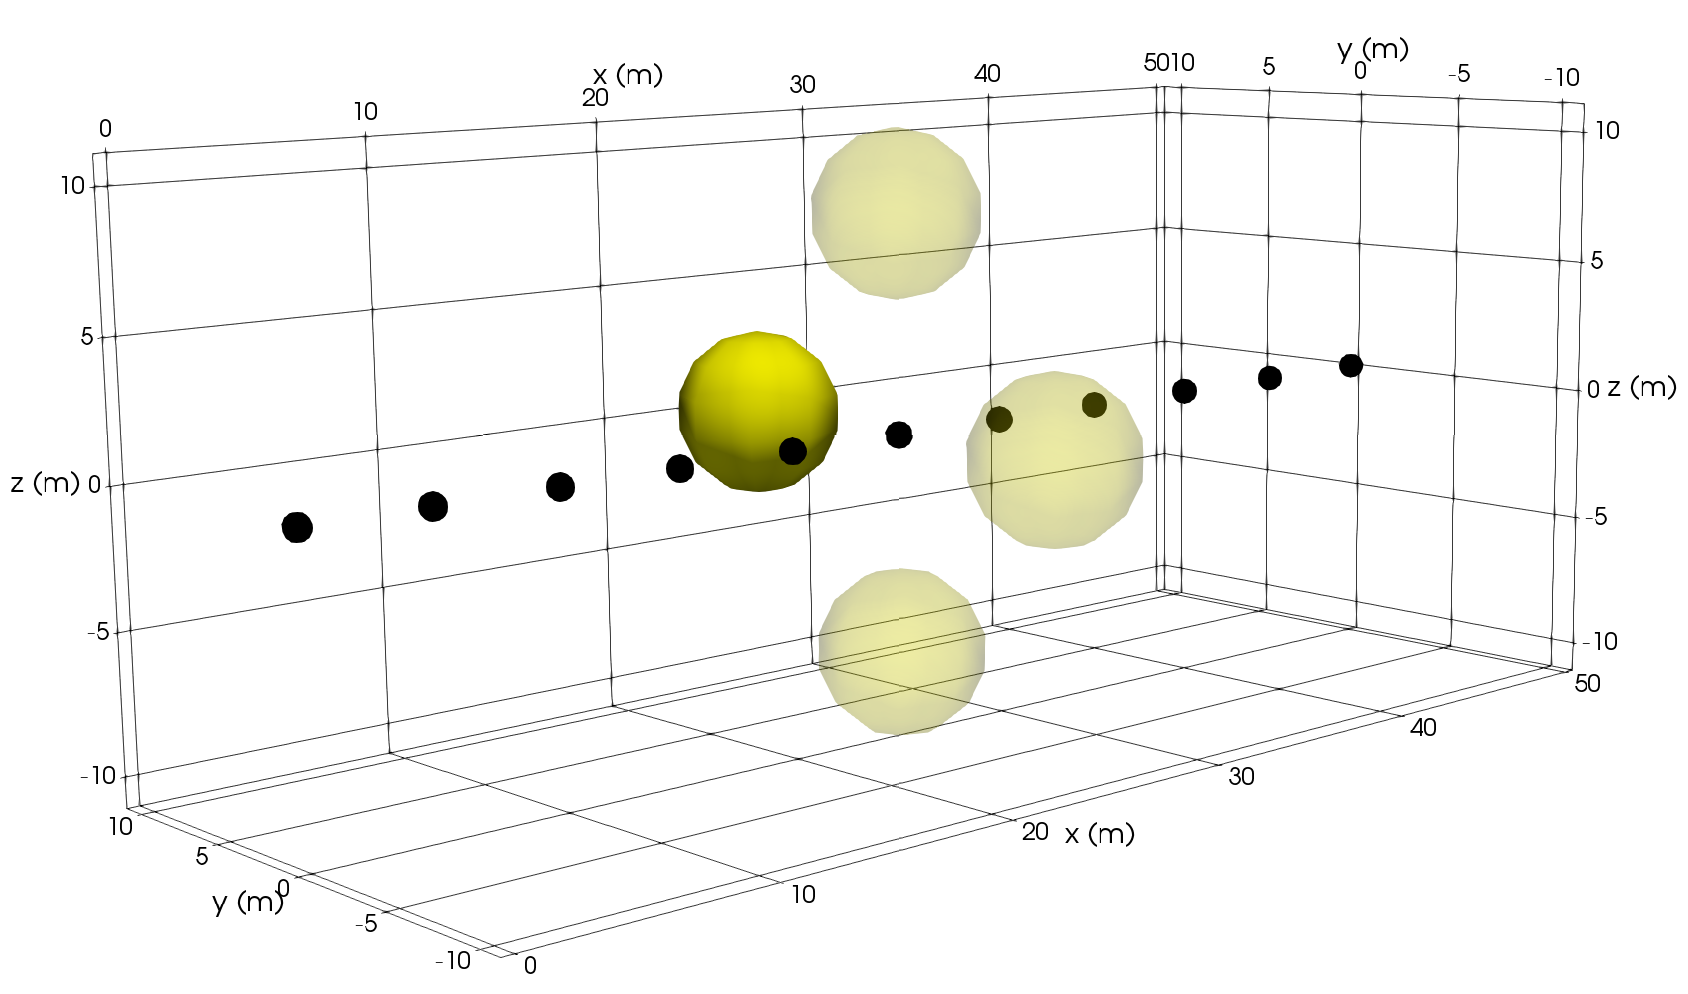
\includegraphics[trim=0cm 0.0cm 0cm 0.0cm, clip=true,width=0.65\linewidth]{./Fig1.png}
   \DIFaddendFL \end{center}
\caption{Oblique view of the experimental setup for a linear array of electrodes embedded in a fullspace. The analytic response of a pole-pole survey with the TX electrode at (25\DIFdelbeginFL \DIFdelFL{m}\DIFdelendFL , 0\DIFdelbeginFL \DIFdelFL{m}\DIFdelendFL , 0 m) is calculated for 4 separate conductive spheres centered at: (25\DIFdelbeginFL \DIFdelFL{m}\DIFdelendFL , 8\DIFdelbeginFL \DIFdelFL{m}\DIFdelendFL , 0 m), (25\DIFdelbeginFL \DIFdelFL{m}\DIFdelendFL , 0\DIFdelbeginFL \DIFdelFL{m}\DIFdelendFL , 8 m), (25\DIFdelbeginFL \DIFdelFL{m}\DIFdelendFL , -8\DIFdelbeginFL \DIFdelFL{m}\DIFdelendFL , 0 m), and (25\DIFdelbeginFL \DIFdelFL{m}\DIFdelendFL , 0\DIFdelbeginFL \DIFdelFL{m}\DIFdelendFL , -8 m)\DIFaddbeginFL \DIFaddFL{, }\DIFaddendFL respectively. In this Figure Sphere \#1 is solid while the other spheres are translucent.}
\label{fig:4Spheres_ObliqueView}
\end{figure}

To assess the performance of each survey the problem was discretized on an octree mesh with 1 m cubic cells in the core region and a 5 m conductive cube was placed at the same center location as sphere 1 (25\DIFdelbegin \DIFdel{m}\DIFdelend , 8\DIFdelbegin \DIFdel{m}\DIFdelend , 0 m). Synthetic data \DIFdelbegin \DIFdel{was }\DIFdelend \DIFaddbegin \DIFadd{were }\DIFaddend then forward modeled and inverted for each survey. To minimize complicating factors and promote the best possible recovery of the conductive block no noise was added to the forward modeled data and uncertainties were set using only a small floor value of \DIFdelbegin \DIFdel{$1e-6$ }\DIFdelend \DIFaddbegin \DIFadd{$1 \times 10^{\text{-6}}$ }\DIFaddend V/A.


\subsubsection{Trial 1: Single Linear Array}
\label{sec:TheoreticalAnalysis_Trial1_SingleLinearArray}

Due to the symmetry of the single linear array\DIFaddbegin \DIFadd{, }\DIFaddend any sphere of the same radius and conductivity that is centered on the dotted circle in Figure \ref{fig:4Spheres_Symmetric_Model} will produce an identical secondary response, as shown in panel b). Since there is no difference in the modeled data\DIFaddbegin \DIFadd{, }\DIFaddend the inversion has no way to constrain the true location of the sphere.


\begin{figure}[htp]
   \begin{center}
      \begin{subfigure}{0.4\linewidth}
         \DIFdelbeginFL %DIFDELCMD < \includegraphics[trim=0cm 0cm 0cm 0cm, clip=true,width=\linewidth]{./Figures/TheoreticalAnalysis/FourSpheres_SectionX=25.pdf}
%DIFDELCMD <          %%%
\DIFdelendFL \DIFaddbeginFL 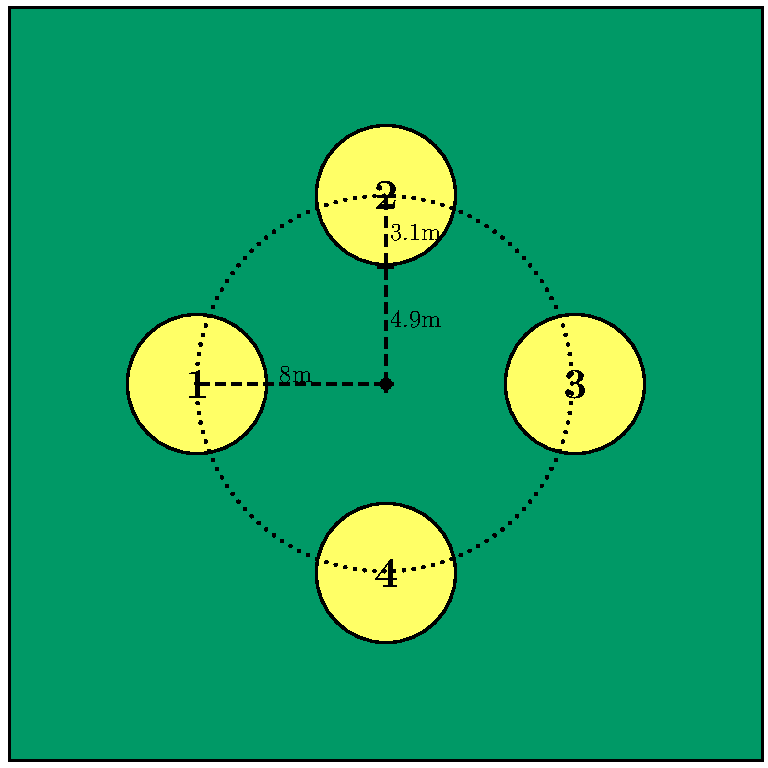
\includegraphics[trim=0cm 0cm 0cm 0cm, clip=true,width=\linewidth]{./Fig2a.pdf}
         \DIFaddendFL \caption{}
         \label{fig:4Spheres_Symmetric_Model}
      \end{subfigure}
      \hfill
      \begin{subfigure}{0.59\linewidth}
         \DIFdelbeginFL %DIFDELCMD < \includegraphics[trim=0cm 0cm 0cm 0cm, clip=true,width=\linewidth]{./Figures/TheoreticalAnalysis/Vs_4sphere_PoleData.pdf}
%DIFDELCMD <          %%%
\DIFdelendFL \DIFaddbeginFL 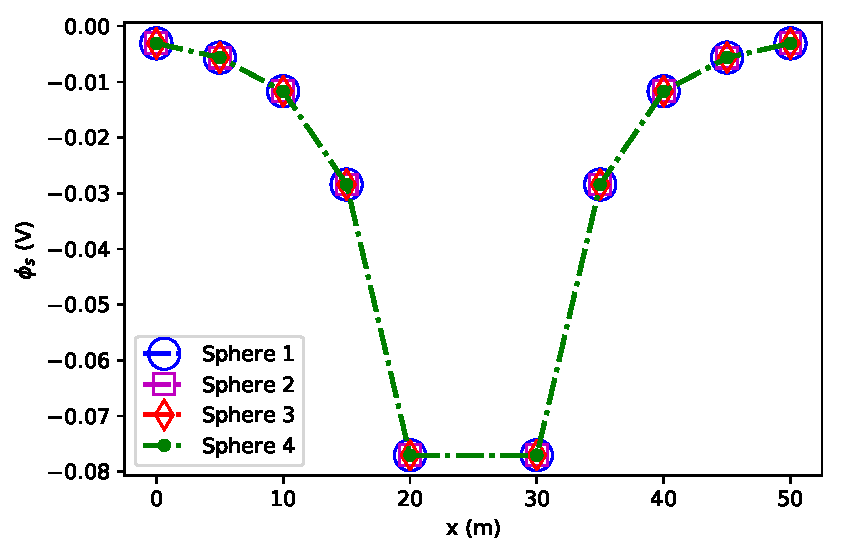
\includegraphics[trim=0cm 0cm 0cm 0cm, clip=true,width=\linewidth]{./Fig2b.pdf}
         \DIFaddendFL \caption{}
         \label{fig:4Spheres_Symmetric_Vs}
      \end{subfigure}
   \end{center}
\caption{Panel \ref{fig:4Spheres_Symmetric_Model} shows the location of the conductive (yellow) spheres laid out symmetrically around the linear array of electrodes (black dots)\DIFaddbeginFL \DIFaddFL{, }\DIFaddendFL which extends into and out of the page. Panel \ref{fig:4Spheres_Symmetric_Vs} shows the secondary potentials at the pole RX locations for each of the 4 spheres. As a result of the symmetry, the measured response of each sphere is identical.}
\label{fig:4Spheres_Symmetric}
\end{figure}


The first row of plots in Figure \ref{fig:SurveyDesign_SLA_Blk_8mSide_NoTunnel_OffsetTX_Trials_XZSections} shows how this fundamental non-uniqueness in measured potentials translates into the recovered inversion model. While the inversion of the single linear array can determine the along array location ($x$-location) of the anomalous body it was unable to constrain the around array location ($y$ and $z$-location) of the conductive cube. In the recovered model the conductive anomaly forms a circular ring around the electrode array. Dealing with this non-uniqueness requires modification of the survey design to break the symmetry inherent to the single linear array.


%DIF <  \begin{figure}[htp]
%DIF <      \begin{center}
%DIF <          \includegraphics[trim=0cm 0cm 0cm 0cm, clip=true,width=\linewidth]{./Figures/TheoreticalAnalysis/InvMod_SingleLinearArray_SingleBlk_Center8mSide_NoTunnel_1TxPP_XZ.pdf}
%DIF <      \end{center}
%DIF <  \caption{}
%DIF <  \label{fig:InvMod_SLA_Blk_8mSide_NoTunnel_1TXPP_XZ}
%DIF <  \end{figure}
\DIFdelbegin %DIFDELCMD <

%DIFDELCMD < %%%
\DIFdelend \subsubsection{Trial 2: Linear Array of RXs with an Electrode Offset in the Y or Z Direction}
\label{sec:TheoreticalAnalysis_Trial2_SingleElecOffset}

To break the symmetry of the single linear array a single electrode was added to the array\DIFaddbegin \DIFadd{, }\DIFaddend which is offset in either the $y$ or $z$\DIFdelbegin \DIFdel{directions}\DIFdelend \DIFaddbegin \DIFadd{-direction}\DIFaddend . Figure \ref{fig:4Spheres_TX_ZOffset} shows the results of offsetting the TX electrode by 2 m in the positive $z$\DIFdelbegin \DIFdel{direction }\DIFdelend \DIFaddbegin \DIFadd{-direction }\DIFaddend so that it is located at (25\DIFdelbegin \DIFdel{m}\DIFdelend , 0\DIFdelbegin \DIFdel{m}\DIFdelend , 2 m). The pole-pole data profiles in Figure \ref{fig:4Spheres_ZOffset_Vs} show that the $z$ offset TX electrode breaks the symmetry of the linear array since the current source is now closer to sphere 2 than sphere 4. This alters the distribution of the secondary currents and charges enough to produce a measurable difference in the response of spheres 2 and 4. However, the responses of spheres 1 and 3 remain identical since these spheres are still symmetrically positioned with respect to the electrodes. Similarly, if the TX electrode is offset by 2 m in the positive $y$\DIFdelbegin \DIFdel{direction }\DIFdelend \DIFaddbegin \DIFadd{-direction }\DIFaddend (25\DIFdelbegin \DIFdel{m}\DIFdelend , 2\DIFdelbegin \DIFdel{m}\DIFdelend , 0 m) spheres 1 and 3 can be differentiated but spheres 2 and 4 cannot.

\begin{figure}[htp]
   \begin{center}
      \begin{subfigure}{0.4\linewidth}
         \DIFdelbeginFL %DIFDELCMD < \includegraphics[trim=0cm 0cm 0cm 0cm, clip=true,width=\linewidth]{./Figures/TheoreticalAnalysis/FourSpheres_SectionX=25_TX_ZOffset.pdf}
%DIFDELCMD <          %%%
\DIFdelendFL \DIFaddbeginFL 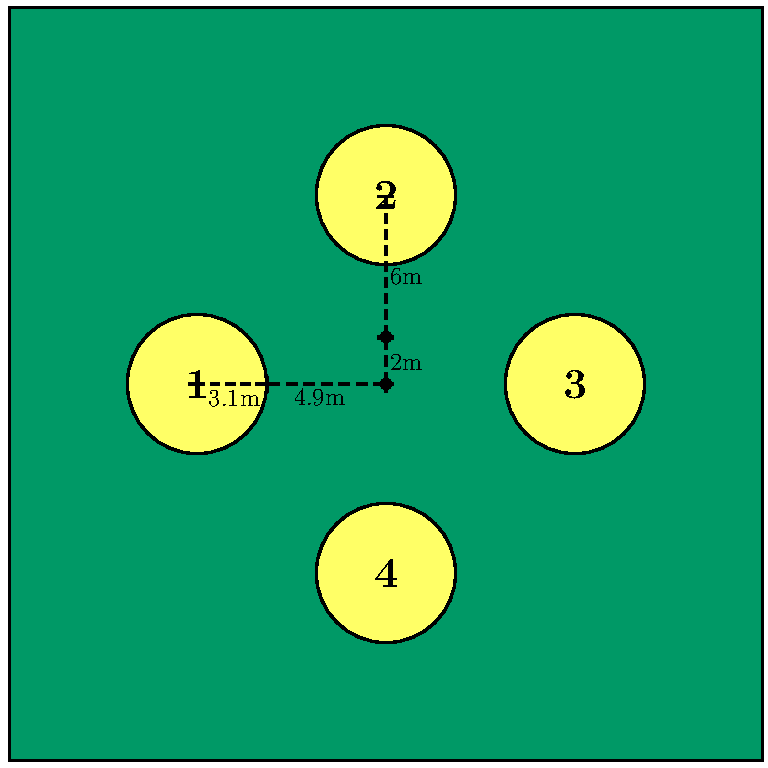
\includegraphics[trim=0cm 0cm 0cm 0cm, clip=true,width=\linewidth]{./Fig3a.pdf}
         \DIFaddendFL \caption{}
         \label{fig:4Spheres_ZOffset_Model}
      \end{subfigure}
      \hfill
      \begin{subfigure}{0.59\linewidth}
         \DIFdelbeginFL %DIFDELCMD < \includegraphics[trim=0cm 0cm 0cm 0cm, clip=true,width=\linewidth]{./Figures/TheoreticalAnalysis/Vs_4sphere_PoleData_TX_ZOffset.pdf}
%DIFDELCMD <          %%%
\DIFdelendFL \DIFaddbeginFL 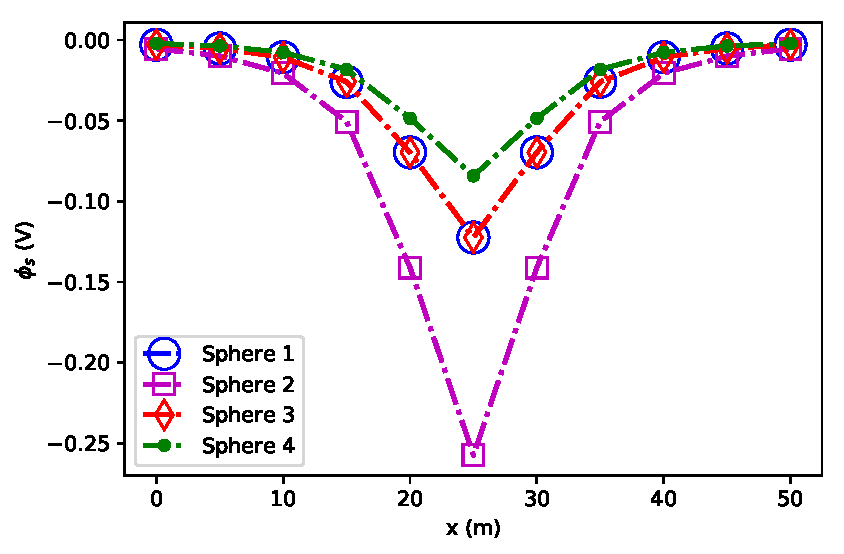
\includegraphics[trim=0cm 0cm 0cm 0cm, clip=true,width=\linewidth]{./Fig3b.pdf}
         \DIFaddendFL \caption{}
         \label{fig:4Spheres_ZOffset_Vs}
      \end{subfigure}
   \end{center}
\caption{Panel \ref{fig:4Spheres_ZOffset_Model} shows the location of the conductive (yellow) spheres laid out symmetrically around the linear array of RX electrodes\DIFaddbeginFL \DIFaddFL{, }\DIFaddendFL which extends into and out of the page. An additional electrode, which is offset by 2 m in the \DIFdelbeginFL \DIFdelFL{$+z$  direction }\DIFdelendFL \DIFaddbeginFL \DIFaddFL{positive $z$-direction, }\DIFaddendFL has been inserted at (25\DIFdelbeginFL \DIFdelFL{m}\DIFdelendFL , 0\DIFdelbeginFL \DIFdelFL{m}\DIFdelendFL , 2 m) for the TX electrode. Panel \ref{fig:4Spheres_ZOffset_Vs} shows the secondary potentials at the pole RX locations for each of the 4 spheres. The $z$ offset of the TX electrode allows us to differentiate the response of spheres 2 and 4. The response of spheres 1 and 3 remain identical\DIFaddbeginFL \DIFaddFL{, }\DIFaddendFL however, since they are symmetrically positioned relative to the electrodes.}
\label{fig:4Spheres_TX_ZOffset}
\end{figure}

Using the same mesh and model from Trial 1, data \DIFdelbegin \DIFdel{was }\DIFdelend \DIFaddbegin \DIFadd{were }\DIFaddend forward modeled and inverted for these surveys with a single offset TX. Sections from the $z$ offset TX inversion model are shown in the second row of Figure \ref{fig:SurveyDesign_SLA_Blk_8mSide_NoTunnel_OffsetTX_Trials_XZSections}. In this inversion, the conductive anomaly is preferentially placed in close proximity to the offset current electrode above the electrode array instead of its true location to the side of the array. This type of artifact clearly shows that having a measurable difference in the recorded data is a necessary but not sufficient condition for addressing this particular model non-uniqueness problem. In addition to having measurable differences between each of the 4 spheres the distribution of sensitivities also needs to be considered.

The sensitivity $\left( J \right)$ is a measure of the change in the $i$th datum as a result of a unit change in the $j$th model cell $\left( J_{ij} = \frac{\partial d_i}{\partial m_j} \right)$. Since measurements are more sensitive to conductivity changes in close proximity to the electrode locations\DIFaddbegin \DIFadd{, }\DIFaddend the inversion preferentially adds structure in these high sensitivity regions to reduce the data misfit $\left( \phi_d \right)$ while minimizing the smallness term of the model objective function $\left( \phi_m \right)$. \citet{McGILLIVRAY1990} and \citet{Spitzer1998} further discuss theoretical aspects of sensitivity and the main ways to compute it.


%DIF <  These inversion results show that the recovered anomaly is placed on the side of the array closest to the TX where the sensitivity is the highest.
\DIFdelbegin %DIFDELCMD <

%DIFDELCMD < %%%
%DIF <  \begin{figure}[htp]
%DIF <      \begin{center}
%DIF <          \includegraphics[trim=0cm 0cm 0cm 0cm, clip=true,width=\linewidth]{./Figures/TheoreticalAnalysis/InvMod_SingleLinearArray_SingleBlk_Center8mSide_NoTunnel_1TxPP_ZOffset_XZ.pdf}
%DIF <      \end{center}
%DIF <  \caption{}
%DIF <  \label{fig:InvMod_SLA_Blk_8mSide_NoTunnel_1TXPP_ZOffset_XZ}
%DIF <  \end{figure}
%DIFDELCMD <

%DIFDELCMD < %%%
\DIFdelend \subsubsection{Trial 3: Linear Array of RX with 2 Orthogonal Offset Electrodes}
\label{sec:TheoreticalAnalysis_Trial3_2OrthogElecOffset}

To slowly build up the complexity of the survey, one of the $y$ and $z$ single offset TX datasets are now combined. The combined survey has 2 TXs and 20 data. Since Trial 2 showed that the data from the $y$ offset TX can differentiate sphere/block 1 and 3 and the data from the $z$ offset TX can differentiate sphere/block 2 and 4 the combined dataset should have the ability to differentiate the responses of conductive anomalies in any of these locations. The inversion results of a \DIFdelbegin \DIFdel{$-y$ }\DIFdelend \DIFaddbegin \DIFadd{-$y$ }\DIFaddend and $+z$ offset TX dataset are shown in the third row of Figure \ref{fig:SurveyDesign_SLA_Blk_8mSide_NoTunnel_OffsetTX_Trials_XZSections}. This result shows that if neither of the electrodes is offset in the same direction as the conductive block, then the recovered conductive anomaly is centered about the closer TX and is smeared out \DIFdelbegin \DIFdel{towards }\DIFdelend \DIFaddbegin \DIFadd{toward }\DIFaddend the true location of the conductive block. This misleading inversion result once again appears to be a result of asymmetric sensitivity bias. When there is a transmitter near the conductive block, the measured secondary potentials are larger and sensitivity bias appears to have a smaller impact on the recovered model.


%DIF <  \begin{figure}[htp]
%DIF <      \begin{center}
%DIF <          \includegraphics[trim=0cm 0cm 0cm 0cm, clip=true,width=\linewidth]{./Figures/TheoreticalAnalysis/InvMod_SingleLinearArray_SingleBlk_Center8mSide_NoTunnel_1TxPP_-YZOffset_XZ.pdf}
%DIF <      \end{center}
%DIF <  \caption{}
%DIF <  \label{fig:InvMod_SLA_Blk_8mSide_NoTunnel_1TXPP_-YZOffset_XZ}
%DIF <  \end{figure}
\DIFdelbegin %DIFDELCMD <

%DIFDELCMD < %%%
\DIFdelend \subsubsection{Trial 4: Linear Array of RX with 4 Orthogonal Offset Electrodes}
\label{sec:TheoreticalAnalysis_Trial4_4OrthogElecOffset}
Two more offset TX datasets were then added to form a survey with 4 orthogonal offset TX electrodes. The resulting survey contained 4 TXs and 40 data. This survey was then tested to see if the symmetric distribution of sensitivities would help minimize the artifacts and smearing that were observed in the inversion results of previous trials. The fourth row of Figure \ref{fig:SurveyDesign_SLA_Blk_8mSide_NoTunnel_OffsetTX_Trials_XZSections} shows section views of the greatly improved inversion model. In this recovered model the location of the conductive block to the north of the electrode array is unambiguously identified and there is no visible smearing of the conductive anomaly around the electrode array.


%DIF <  \begin{figure}[htp]{}
%DIF <      \begin{center}
%DIF <          \begin{subfigure}{0.49\linewidth}
%DIF <              \includegraphics[trim=0cm 0cm 0cm 0cm, clip=true,width=\linewidth]{./Figures/TheoreticalAnalysis/InvMod_SingleLinearArray_SingleBlk_Center8mSide_NoTunnel_1TXPP_X=25.pdf}
%DIF <              \label{fig:InvMod_SLA_Blk_8mSide_NoTunnel_1TXPP_X}
%DIF <              \caption{Single Linear Array}
%DIF <          \end{subfigure}\hspace{-0.8cm}
%DIF <          \qquad
%DIF <          \begin{subfigure}{0.49\linewidth}
%DIF <              \includegraphics[trim=0cm 0cm 0cm 0cm, clip=true,width=\linewidth]{./Figures/TheoreticalAnalysis/InvMod_SingleLinearArray_SingleBlk_Center8mSide_NoTunnel_1TXPP_+ZOffset_X=25.pdf}
%DIF <              \label{fig:InvMod_SLA_Blk_8mSide_NoTunnel_1TXPP_+ZOffset_X}
%DIF <              \caption{$+z$ Offset TX}
%DIF <          \end{subfigure}\hspace{-0.8cm}
\DIFdelbegin %DIFDELCMD <

%DIFDELCMD < %%%
%DIF <          \begin{subfigure}{0.49\linewidth}
%DIF <              \includegraphics[trim=0cm 0cm 0cm 0cm, clip=true,width=\linewidth]{./Figures/TheoreticalAnalysis/InvMod_SingleLinearArray_SingleBlk_Center8mSide_NoTunnel_1TXPP_-YZOffset_X=25.pdf}
%DIF <              \label{fig:InvMod_SLA_Blk_8mSide_NoTunnel_1TXPP_-YZOffset_X}
%DIF <              \caption{$-y$ and $+z$ Offset TXs}
%DIF <          \end{subfigure}\hspace{-0.8cm}
%DIF <          \qquad
%DIF <          \begin{subfigure}{0.49\linewidth}
%DIF <              \includegraphics[trim=0cm 0cm 0cm 0cm, clip=true,width=\linewidth]{./Figures/TheoreticalAnalysis/InvMod_SLA_Blk_8mSide_NoTunnel_4TXPP_AllYZOffset_X=25.pdf}
%DIF <              \label{fig:InvMod_SLA_Blk_8mSide_NoTunnel_4TXPP_AllYZOffset_X}
%DIF <              \caption{4 Orthogonal Offset TXs}
%DIF <          \end{subfigure}\hspace{-0.8cm}
%DIFDELCMD <

%DIFDELCMD < %%%
%DIF <      \end{center}
%DIF <  \vspace{-0.55cm}
%DIF <  \caption{}
%DIF <  \label{fig:InvMod_StraightTunnel_OffsetTX_X=25_Comp}
%DIF <  \end{figure}
%DIFDELCMD <

%DIFDELCMD < %%%
\DIFdelend \begin{figure}[htp]{}
\captionsetup[subfigure]{labelformat=empty}
   \begin{center}
      %DIF <  \begin{subfigure}{0.02\linewidth}
      %DIF <      % Blank Placeholder
      %DIF <  \end{subfigure}\hspace{-0.8cm}
      %DIF <  \qquad
      %DIF <  \begin{subfigure}{0.44\linewidth}
      %DIF <      \begin{picture}(100,0)
      %DIF <           \put(56,0){\scriptsize{\textbf{X Section}}}
      %DIF <     \end{picture}
      %DIF <  \end{subfigure}\hspace{-0.8cm}
      %DIF <  \qquad
      %DIF <  \begin{subfigure}{0.44\linewidth}
      %DIF <      \begin{picture}(100,0)
      %DIF <           \put(52,0){\scriptsize{\textbf{Z Section}}}
      %DIF <     \end{picture}
      %DIF <  \end{subfigure}\hspace{-0.8cm}
\DIFdelbeginFL %DIFDELCMD <

%DIFDELCMD <       %%%
\DIFdelendFL \vspace{0.1cm}
      \begin{subfigure}{0.02\linewidth}
        \DIFdelbeginFL %DIFDELCMD < \begin{center}
%DIFDELCMD <             %%%
\DIFdelendFL \begin{turn}{90}
          \DIFdelbeginFL %DIFDELCMD < \scriptsize{\textbf{Single Linear Array}}
%DIFDELCMD <             %%%
\DIFdelendFL \DIFaddbeginFL \begin{picture}(100,0)
            \put(30,0){\scriptsize{\textbf{Single Linear Array}}}
          \end{picture}
        \DIFaddendFL \end{turn}
      \DIFdelbeginFL %DIFDELCMD < \end{center}
%DIFDELCMD <       %%%
\DIFdelendFL \end{subfigure}\hspace{-0.8cm}
      \qquad
      \begin{subfigure}{0.825\linewidth}
         \label{fig:SurveyDesign_SLA_Blk_8mSide_NoTunnel_1TXPP_XZ}
         \DIFdelbeginFL %DIFDELCMD < \includegraphics[trim=0cm 0cm 0cm 0cm, clip=true,width=\linewidth]{./Figures/TheoreticalAnalysis/InvMod_SingleLinearArray_SingleBlk_Center8mSide_NoTunnel_1TXPP_XZ.pdf}
%DIFDELCMD <       %%%
\DIFdelendFL \DIFaddbeginFL 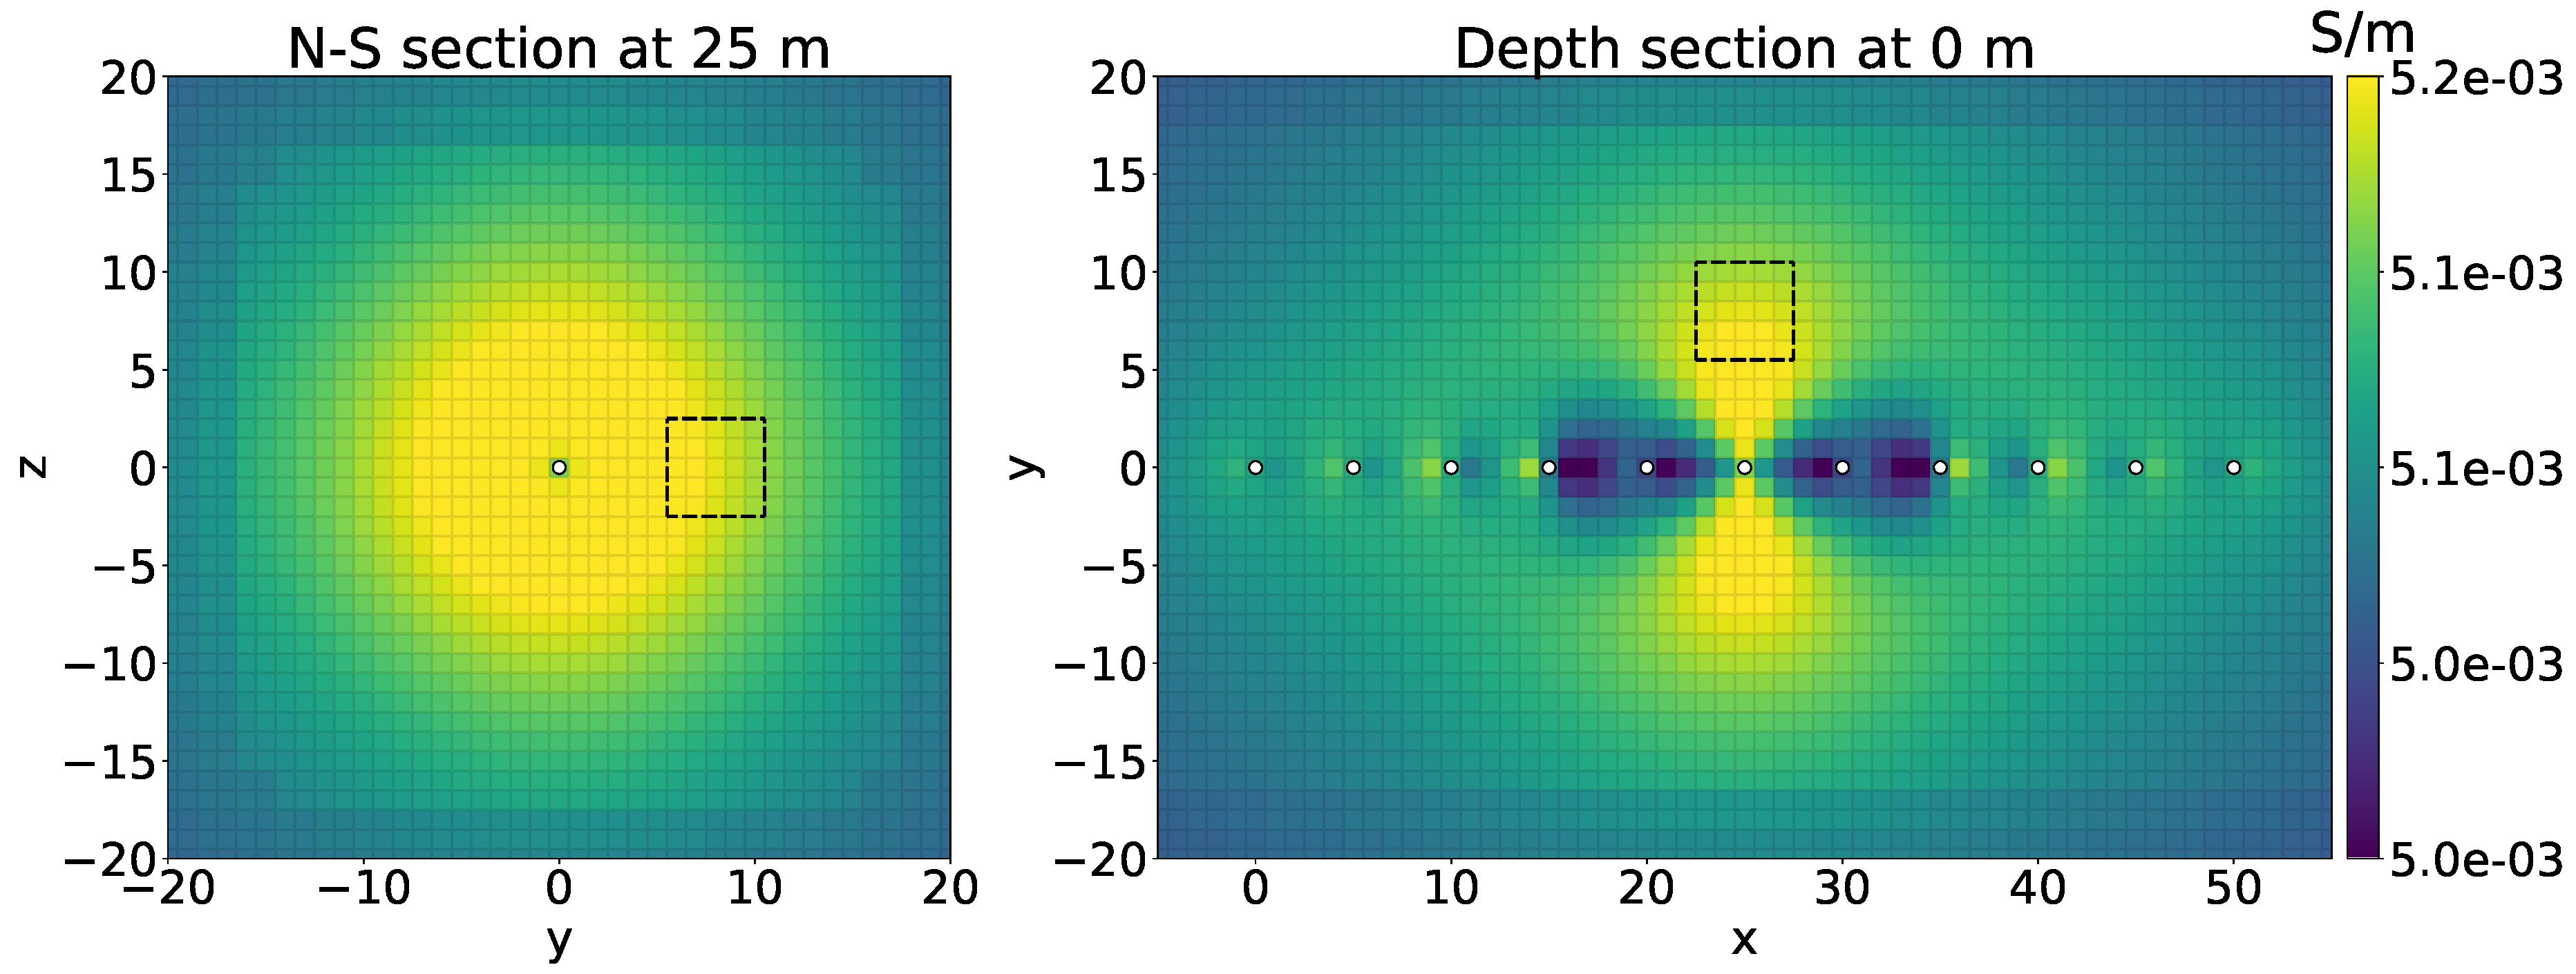
\includegraphics[trim=0cm 0cm 0cm 0cm, clip=true,width=\linewidth]{./Fig4a.pdf}
      \DIFaddendFL \end{subfigure}

      \begin{subfigure}{0.02\linewidth}
        \DIFdelbeginFL %DIFDELCMD < \begin{center}
%DIFDELCMD <             %%%
\DIFdelendFL \begin{turn}{90}
          \DIFdelbeginFL %DIFDELCMD < \scriptsize{\textbf{$+z$ Offset TX}}
%DIFDELCMD <             %%%
\DIFdelendFL \DIFaddbeginFL \begin{picture}(100,0)
            \put(40,0){\scriptsize{\textbf{$+z$ Offset TX}}}
          \end{picture}
        \DIFaddendFL \end{turn}
      \DIFdelbeginFL %DIFDELCMD < \end{center}
%DIFDELCMD <       %%%
\DIFdelendFL \end{subfigure}\hspace{-0.8cm}
      \qquad
      \begin{subfigure}{0.825\linewidth}
         \label{fig:SurveyDesign_SLA_Blk_8mSide_NoTunnel_1TXPP_+ZOffset_XZ}
         \DIFdelbeginFL %DIFDELCMD < \includegraphics[trim=0cm 0cm 0cm 0cm, clip=true,width=\linewidth]{./Figures/TheoreticalAnalysis/InvMod_SingleLinearArray_SingleBlk_Center8mSide_NoTunnel_1TXPP_ZOffset_XZ.pdf}
%DIFDELCMD <       %%%
\DIFdelendFL \DIFaddbeginFL 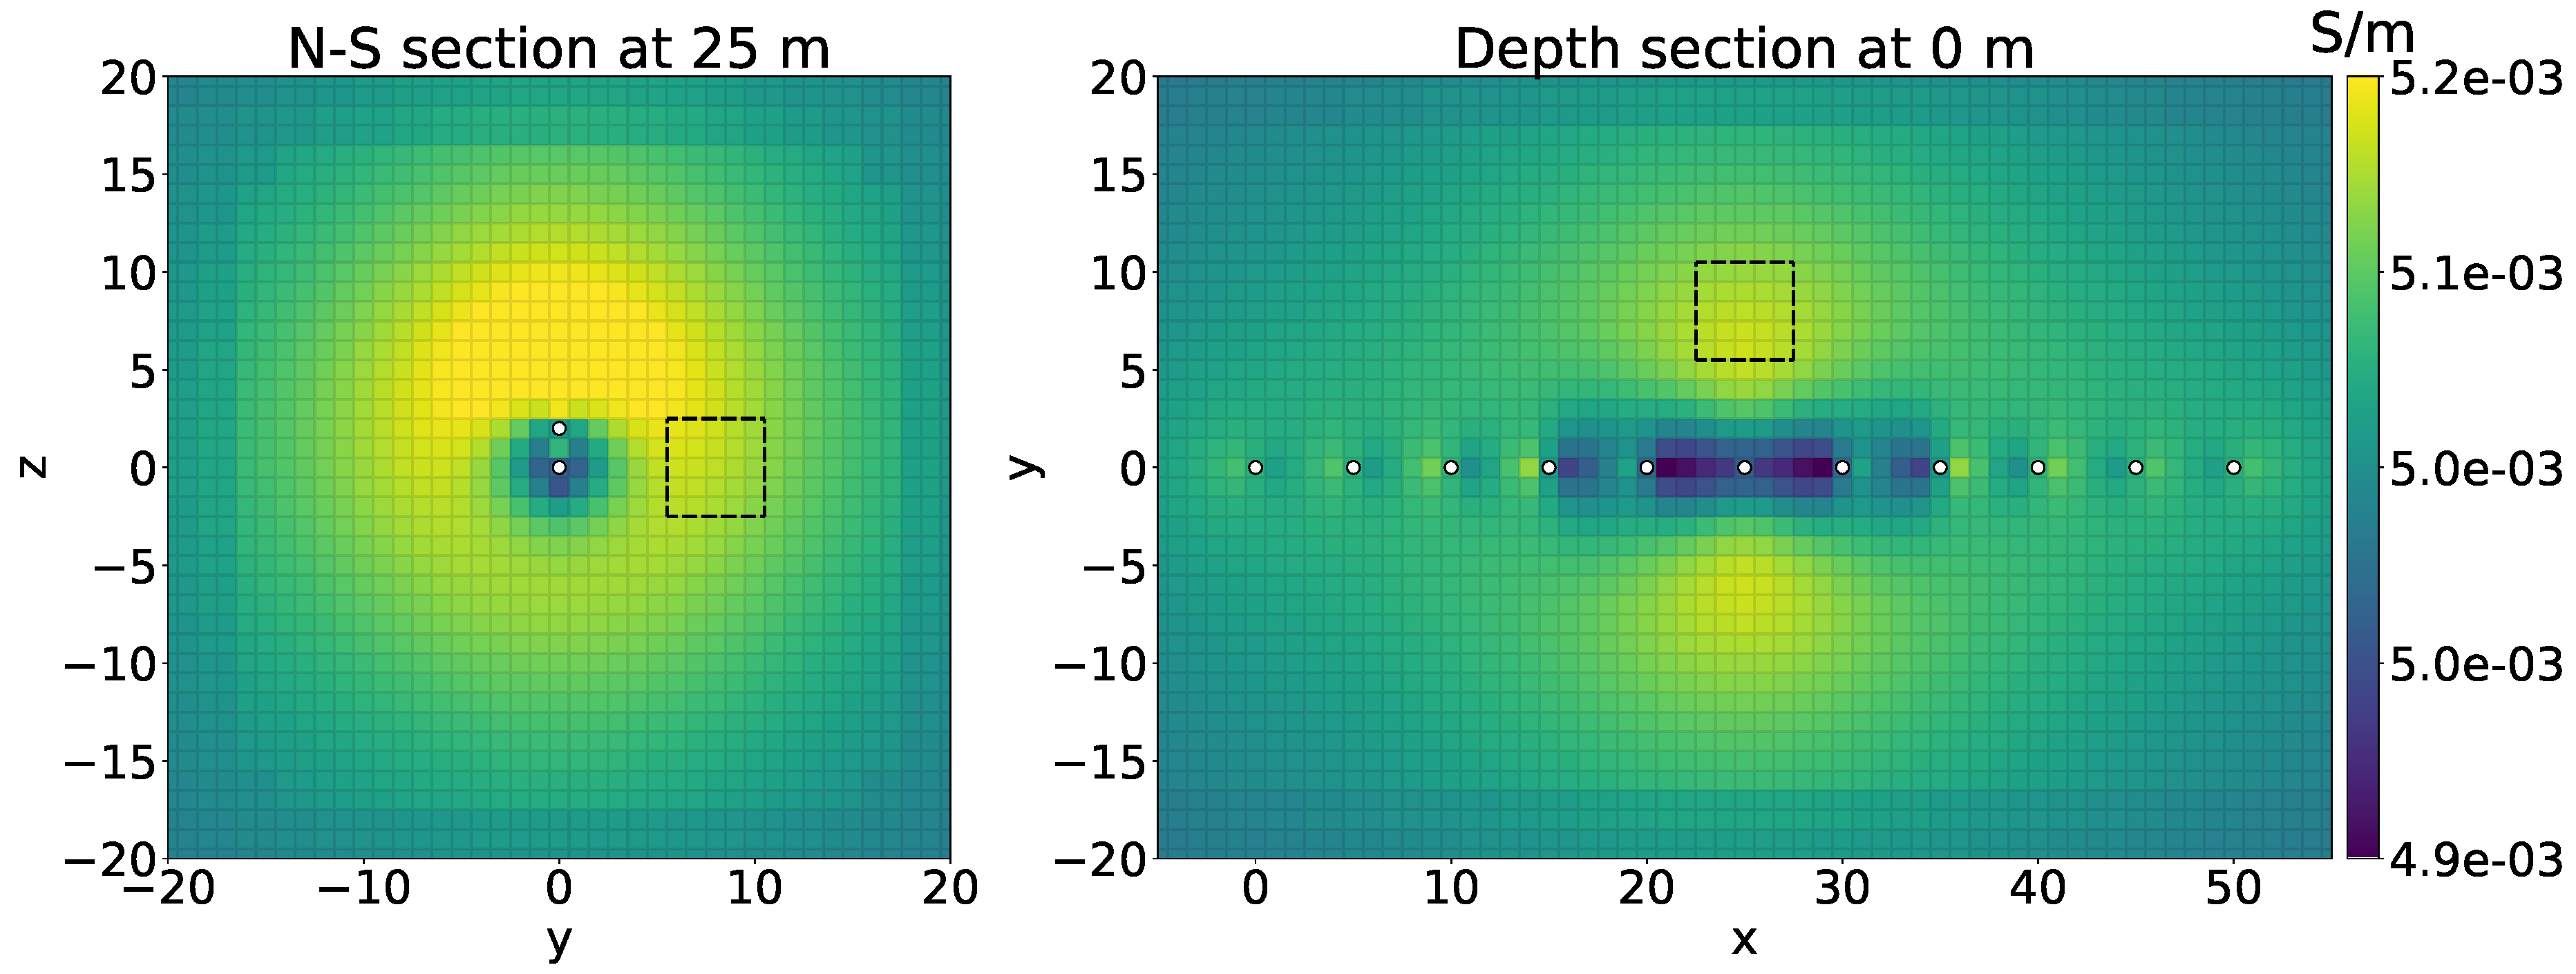
\includegraphics[trim=0cm 0cm 0cm 0cm, clip=true,width=\linewidth]{./Fig4b.pdf}
      \DIFaddendFL \end{subfigure}

      \begin{subfigure}{0.02\linewidth}
        \DIFdelbeginFL %DIFDELCMD < \begin{center}
%DIFDELCMD <             %%%
\DIFdelendFL \begin{turn}{90}
          \DIFdelbeginFL %DIFDELCMD < \scriptsize{\textbf{$-y$ and $+z$ Offset TXs}}
%DIFDELCMD <             %%%
\DIFdelendFL \DIFaddbeginFL \begin{picture}(100,0)
            \put(24,0){\scriptsize{\textbf{-$y$ and $+z$ Offset TXs}}}
          \end{picture}
        \DIFaddendFL \end{turn}
      \DIFdelbeginFL %DIFDELCMD < \end{center}
%DIFDELCMD <       %%%
\DIFdelendFL \end{subfigure}\hspace{-0.8cm}
      \qquad
      \begin{subfigure}{0.825\linewidth}
         \label{fig:SurveyDesign_SLA_Blk_8mSide_NoTunnel_1TXPP_-YZOffset_XZ}
         \DIFdelbeginFL %DIFDELCMD < \includegraphics[trim=0cm 0cm 0cm 0cm, clip=true,width=\linewidth]{./Figures/TheoreticalAnalysis/InvMod_SingleLinearArray_SingleBlk_Center8mSide_NoTunnel_1TXPP_-YZOffset_XZ.pdf}
%DIFDELCMD <       %%%
\DIFdelendFL \DIFaddbeginFL 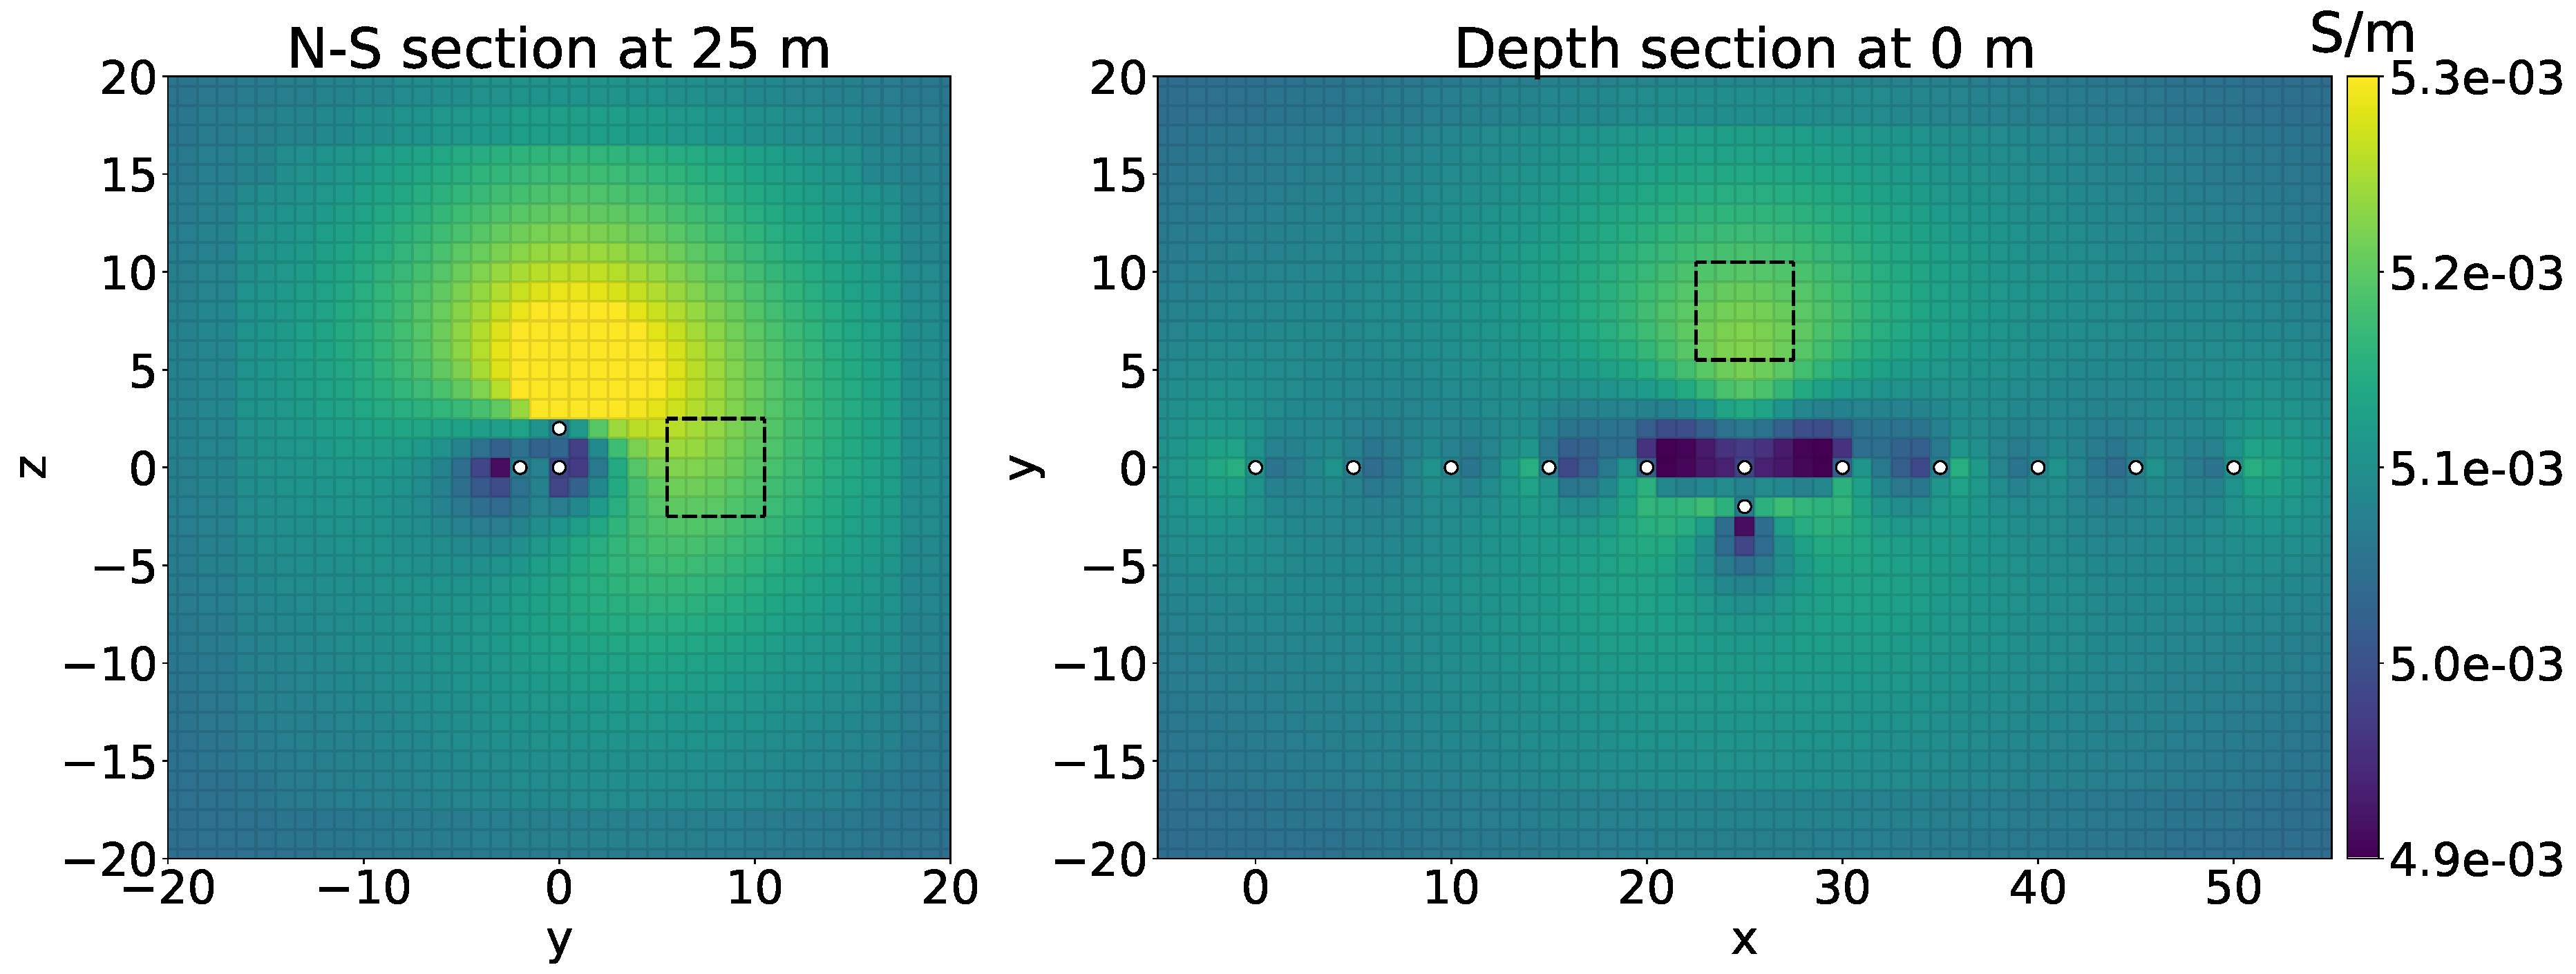
\includegraphics[trim=0cm 0cm 0cm 0cm, clip=true,width=\linewidth]{./Fig4c.pdf}
      \DIFaddendFL \end{subfigure}

      \begin{subfigure}{0.02\linewidth}
        \DIFdelbeginFL %DIFDELCMD < \begin{center}
%DIFDELCMD <             %%%
\DIFdelendFL \begin{turn}{90}
          \DIFdelbeginFL %DIFDELCMD < \scriptsize{\textbf{4 Orthogonal Offset TXs}}
%DIFDELCMD <             %%%
\DIFdelendFL \DIFaddbeginFL \begin{picture}(100,0)
            \put(18,0){\scriptsize{\textbf{4 Orthogonal Offset TXs}}}
          \end{picture}
        \DIFaddendFL \end{turn}
      \DIFdelbeginFL %DIFDELCMD < \end{center}
%DIFDELCMD <       %%%
\DIFdelendFL \end{subfigure}\hspace{-0.8cm}
      \qquad
      \begin{subfigure}{0.825\linewidth}
         \label{fig:SurveyDesign_SLA_Blk_8mSide_NoTunnel_4TXPP_AllYZOffset_XZ}
         \DIFdelbeginFL %DIFDELCMD < \includegraphics[trim=0cm 0cm 0cm 0cm, clip=true,width=\linewidth]{./Figures/TheoreticalAnalysis/InvMod_SLA_Blk_8mSide_NoTunnel_4TXPP_AllYZOffset_XZ.pdf}
%DIFDELCMD <       %%%
\DIFdelendFL \DIFaddbeginFL 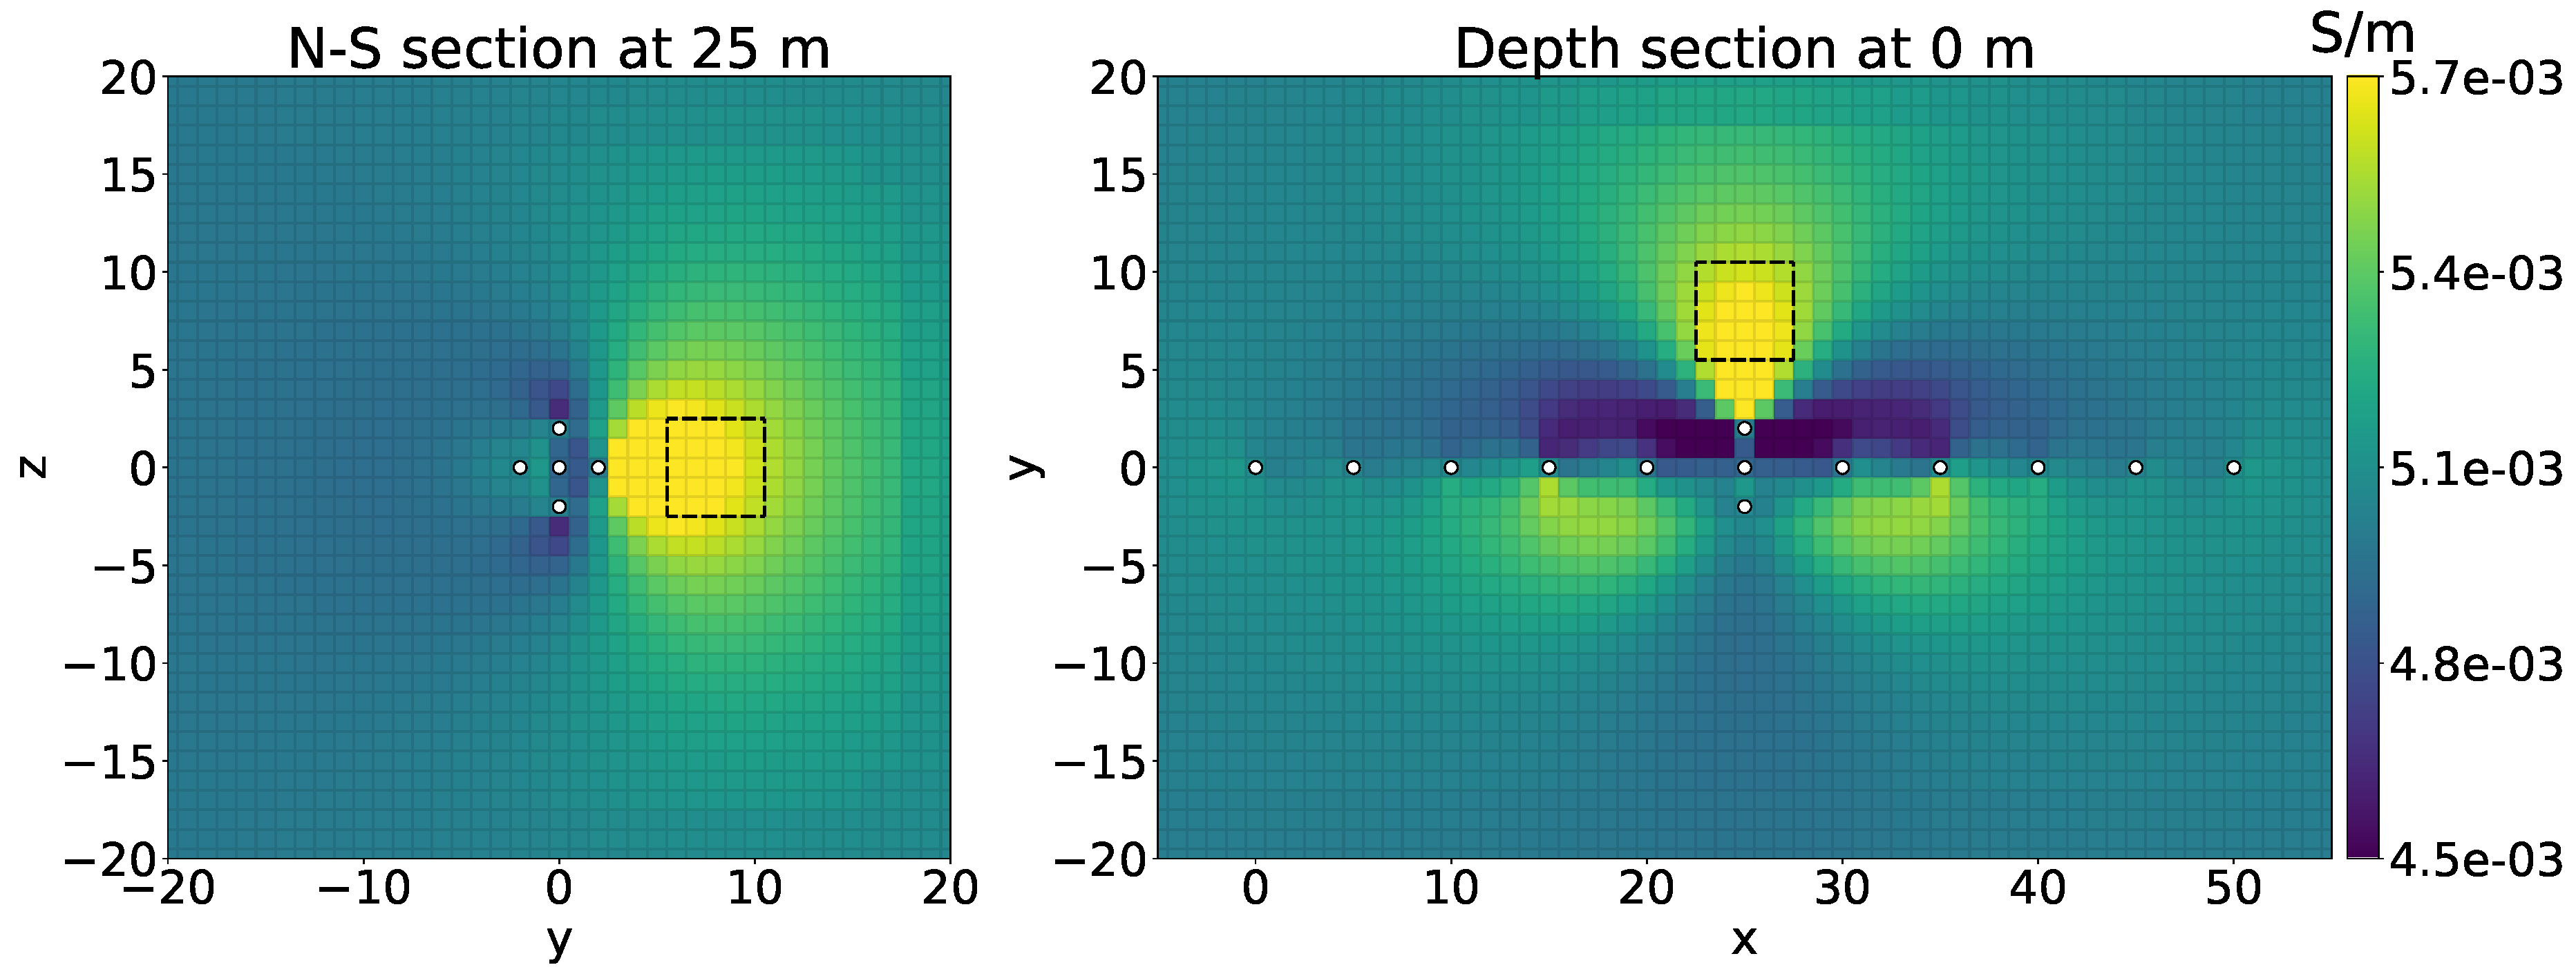
\includegraphics[trim=0cm 0cm 0cm 0cm, clip=true,width=\linewidth]{./Fig4d.pdf}
      \DIFaddendFL \end{subfigure}
   \end{center}
\vspace{-0.6cm}
\caption{\DIFaddbeginFL \DIFaddFL{A series of }\DIFaddendFL $x$ and $z$ sections through the recovered models \DIFdelbeginFL \DIFdelFL{show }\DIFdelendFL \DIFaddbeginFL \DIFaddFL{showing }\DIFaddendFL how our ability to constrain the location of a conductive block off to the side of the tunnel changes depending on the use of different offset TXs. The white dots are projections of the electrode locations onto the section and the black dashed outlines show the edges of structures in the true model.}
\label{fig:SurveyDesign_SLA_Blk_8mSide_NoTunnel_OffsetTX_Trials_XZSections}
\end{figure}



\subsection{Tunnel Effects}
\label{sec:TheoreticalAnalysis_TunnelEffects}

After considering the symmetry related non-uniqueness issues discussed illustrated by Trials 1-4, a simple experiment akin to the 4 sphere trials was designed to show how the presence of a tunnel impacts the ability of a linear array of electrodes to constrain the around-tunnel location of a conductive body. In this experiment, a 3 $\times$ 3 m tunnel is centered about the origin and extends along $x$-axis in the positive and negative directions. As in the previous trials, a linear array of electrodes is used with electrodes placed every 5 m from $x$ = 0 m to $x$ = 50 m in the ceiling of the tunnel. A pole TX is placed in the center of the array, at a location of (25\DIFdelbegin \DIFdel{m}\DIFdelend , 0\DIFdelbegin \DIFdel{m}\DIFdelend , 2 m) and the remaining 10 electrode locations are used as pole RXs. Four separate conductivity models were then created, each containing a 5 m conductive (10 S/m) cube centered 8 m away from the electrode array. Blocks 1 to 4 are centered about: (25\DIFdelbegin \DIFdel{m}\DIFdelend , -8\DIFdelbegin \DIFdel{m}\DIFdelend , 2 m), (25\DIFdelbegin \DIFdel{m}\DIFdelend , 0\DIFdelbegin \DIFdel{m}\DIFdelend , 10 m), (25\DIFdelbegin \DIFdel{m}\DIFdelend , 8\DIFdelbegin \DIFdel{m}\DIFdelend , 2 m), and (25\DIFdelbegin \DIFdel{m}\DIFdelend , 0\DIFdelbegin \DIFdel{m}\DIFdelend , -6 m)\DIFaddbegin \DIFadd{, }\DIFaddend respectively. Figure \ref{fig:4Blocks_Tunnel_Model} shows an amalgamated diagram with the location of all 4 conductive (yellow) blocks relative to the resistive (blue) tunnel and electrode array (black dots).


\begin{figure}[htp]
   \begin{center}
      \begin{subfigure}{0.4\linewidth}
         \DIFdelbeginFL %DIFDELCMD < \includegraphics[trim=0cm 0cm 0cm 0cm, clip=true,width=\linewidth]{./Figures/TheoreticalAnalysis/FourBlocks_Tunnel_SectionX=25.pdf}
%DIFDELCMD <          %%%
\DIFdelendFL \DIFaddbeginFL 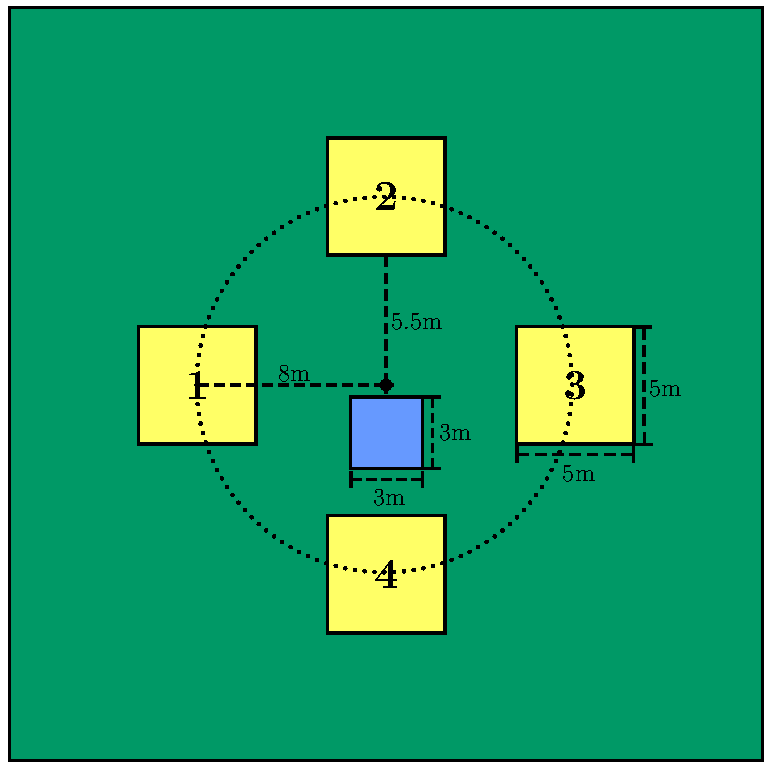
\includegraphics[trim=0cm 0cm 0cm 0cm, clip=true,width=\linewidth]{./Fig5a.pdf}
         \DIFaddendFL \caption{}
         \label{fig:4Blocks_Tunnel_Model}
      \end{subfigure}
      \hfill
      \begin{subfigure}{0.59\linewidth}
         \DIFdelbeginFL %DIFDELCMD < \includegraphics[trim=0cm 0cm 0cm 0cm, clip=true,width=\linewidth]{./Figures/TheoreticalAnalysis/Vs_4Block_Tunnel_PoleData.pdf}
%DIFDELCMD <          %%%
\DIFdelendFL \DIFaddbeginFL 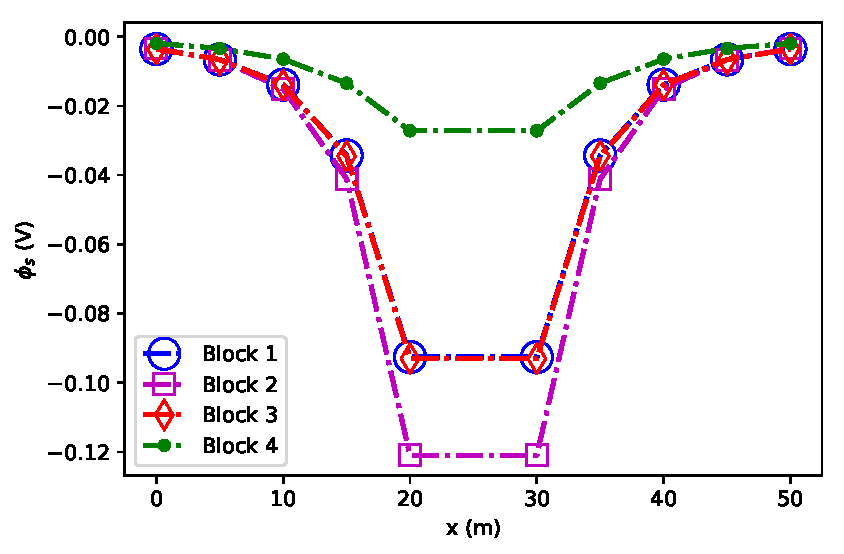
\includegraphics[trim=0cm 0cm 0cm 0cm, clip=true,width=\linewidth]{./Fig5b.pdf}
         \DIFaddendFL \caption{}
         \label{fig:4Blocks_Tunnel_Vs}
      \end{subfigure}
   \end{center}
\caption{Panel \ref{fig:4Blocks_Tunnel_Model} shows the location of the conductive (yellow) 5m cubes laid out symmetrically around the linear array of electrodes (black dot). The electrodes are embedded into the ceiling of the 3 $\times$ 3 m air filled, resistive (blue) tunnel. Both the electrode array and tunnel extend into and out of the page. Panel \ref{fig:4Blocks_Tunnel_Vs} shows the secondary potentials at the pole RX locations for each of the 4 blocks. In this configuration the tunnel breaks the vertical symmetry and allows us to differentiate the response of blocks 2 and 4. Horizontal symmetry is maintained with the single linear array\DIFaddbeginFL \DIFaddFL{, }\DIFaddendFL however\DIFaddbeginFL \DIFaddFL{, }\DIFaddendFL so the secondary response of blocks 1 and 3 are identical.}
\label{fig:4Blocks_Tunnel}
\end{figure}

The much lower secondary response from Block 4, which is on the opposite side of the tunnel as the TX electrode, is due to the current shielding effects of the 3 $\times$ 3 m tunnel\DIFaddbegin \DIFadd{, }\DIFaddend which are illustrated by the current density plots in Figure \ref{fig:J_TunnelEffects_Top_Blk5m_3x3Tunnel_Elec_TopSideBottom}. The tunnel distorts the distribution of primary currents by forcing them to flow around the resistive tunnel. Primary current densities are greatest above the tunnel and diminish as they flow around the tunnel. \DIFdelbegin \DIFdel{This }\DIFdelend \DIFaddbegin \DIFadd{The tunnel }\DIFaddend has a shielding effect on the medium below and to the sides of the tunnel\DIFdelbegin \DIFdel{and }\DIFdelend \DIFaddbegin \DIFadd{, which }\DIFaddend causes conductive bodies in these regions to produce smaller secondary responses. Figure \ref{fig:4Blocks_Tunnel_Vs} summarizes the measured secondary potentials from each of the 4 conductive blocks. These results align with our intuition since block 2, which lies above the TX and tunnel, has the largest amplitude $\phi_{s}$, and $\phi_{s}$ values decrease in magnitude as the block is moved \DIFdelbegin \DIFdel{further }\DIFdelend \DIFaddbegin \DIFadd{farther }\DIFaddend around the tunnel. Since all of the block centers are 8 m away from the pole TX\DIFaddbegin \DIFadd{, }\DIFaddend any variations in $\phi_{s}$ must be solely due to the tunnel.

\begin{figure}[htp]{}
\captionsetup[subfigure]{labelformat=empty}
   \begin{center}
      \begin{subfigure}{0.02\linewidth}
          % Blank Placeholder
      \end{subfigure}\hspace{-0.8cm}
      \qquad
      \begin{subfigure}{0.48\linewidth}{}
          \begin{picture}(100,0)
               \put(77,0){\scriptsize{\textbf{Top of Tunnel}}}
         \end{picture}
      \end{subfigure}\hspace{-0.8cm}
      %DIF <  \qquad
      %DIF <  \begin{subfigure}{0.5\linewidth}
      %DIF <      \begin{picture}(100,0)
      %DIF <           \put(46,0){\scriptsize{\textbf{Side of Tunnel}}}
      %DIF <     \end{picture}
      %DIF <  \end{subfigure}\hspace{-0.8cm}
      \qquad
      \begin{subfigure}{0.48\linewidth}
          \begin{picture}(100,0)
               \put(50,0){\scriptsize{\textbf{Bottom of Tunnel}}}
         \end{picture}
      \end{subfigure}

      \vspace{0.1cm}
      \begin{subfigure}{0.02\linewidth}
        \DIFdelbeginFL %DIFDELCMD < \begin{center}
%DIFDELCMD <             %%%
\DIFdelendFL \begin{turn}{90}
            \DIFdelbeginFL %DIFDELCMD < \scriptsize{\textbf{Primary ($\vec{j_p}$)}}
%DIFDELCMD <             %%%
\DIFdelendFL \DIFaddbeginFL \begin{picture}(100,0)
                \put(65,0){\scriptsize{\textbf{Primary ($\vec{j_p}$)}}}
            \end{picture}
        \DIFaddendFL \end{turn}
      \DIFdelbeginFL %DIFDELCMD < \end{center}
%DIFDELCMD <       %%%
\DIFdelendFL \end{subfigure}\hspace{-0.8cm}
      \qquad
      \begin{subfigure}{0.5\linewidth}
         \label{fig:Jp_SingleLinearArray_Top_Blk5m_8mElecBlkCenter_3x3Tunnel_X3}
         \DIFdelbeginFL %DIFDELCMD < \sbox0{\includegraphics[trim=0cm 0cm 0cm 0cm, clip=true,width=\linewidth]{./Figures/TheoreticalAnalysis/Jp_SingleLinearArray_Bottom_Blk5m_ZLocBlkCenter8m_3x3Tunnel_X=25.png}}
%DIFDELCMD <          \includegraphics[height=\ht0,keepaspectratio]{./Figures/TheoreticalAnalysis/Jp_SingleLinearArray_Top_Blk5m_8mElecBlkCenter_3x3Tunnel_X=25_noCB.png}
%DIFDELCMD <       %%%
\DIFdelendFL \DIFaddbeginFL \sbox0{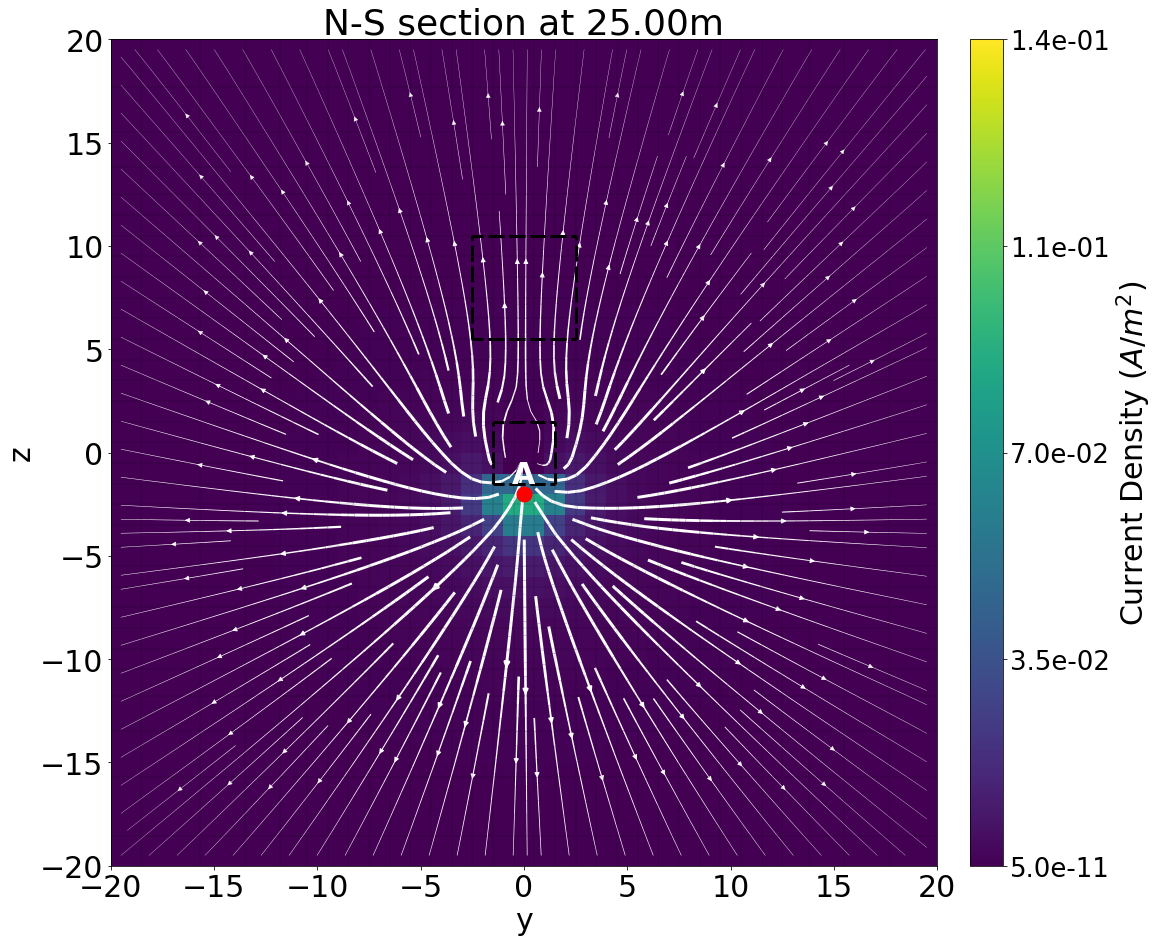
\includegraphics[trim=0cm 0cm 0cm 0cm, clip=true,width=\linewidth]{./Fig6b.png}}
         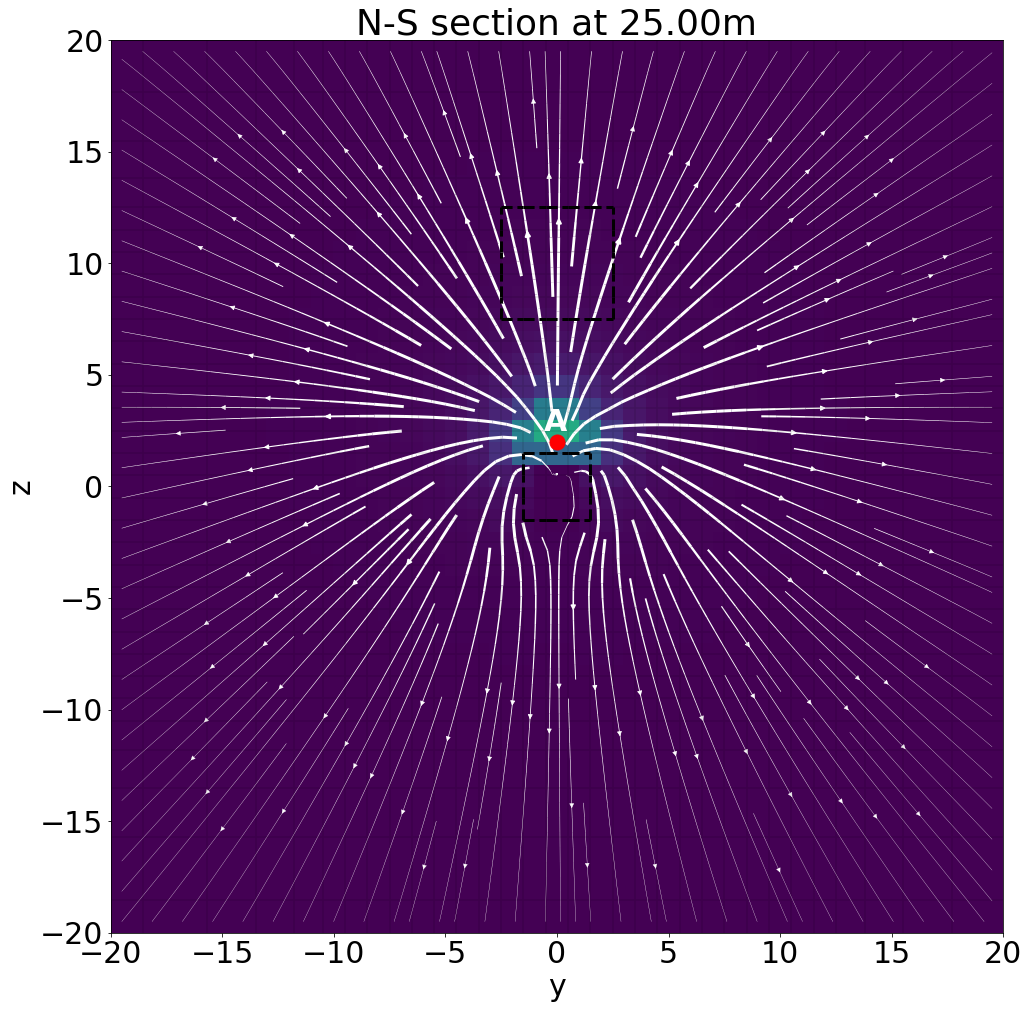
\includegraphics[height=\ht0,keepaspectratio]{./Fig6a.png}
      \DIFaddendFL \end{subfigure}\hspace{-0.9cm}
      %DIF <  \begin{subfigure}{0.5\linewidth}
      %DIF <     \label{fig:Jp_SingleLinearArray_Side_Blk5m_8mElecBlkCenter_3x3Tunnel_X}
      %DIF <     \sbox0{\includegraphics[trim=0cm 0cm 0cm 0cm, clip=true,width=\linewidth]{./Figures/TheoreticalAnalysis/Jp_SingleLinearArray_Side_Blk5m_8mElecBlkCenter_3x3Tunnel_X=25.png}}
      %DIF <     \includegraphics[height=\ht0,keepaspectratio]{./Figures/TheoreticalAnalysis/Jp_SingleLinearArray_Side_Blk5m_8mElecBlkCenter_3x3Tunnel_X=25_noCB.png}
      %DIF <  \end{subfigure}\hspace{-0.9cm}
      \begin{subfigure}{0.5\linewidth}
         \label{fig:Jp_SingleLinearArray_Bottom_Blk5m_ZLocBlkCenter8m_3x3Tunnel_X}
         \DIFdelbeginFL %DIFDELCMD < \includegraphics[trim=0cm 0cm 0cm 0cm, clip=true,width=\linewidth]{./Figures/TheoreticalAnalysis/Jp_SingleLinearArray_Bottom_Blk5m_ZLocBlkCenter8m_3x3Tunnel_X=25.png}
%DIFDELCMD <       %%%
\DIFdelendFL \DIFaddbeginFL 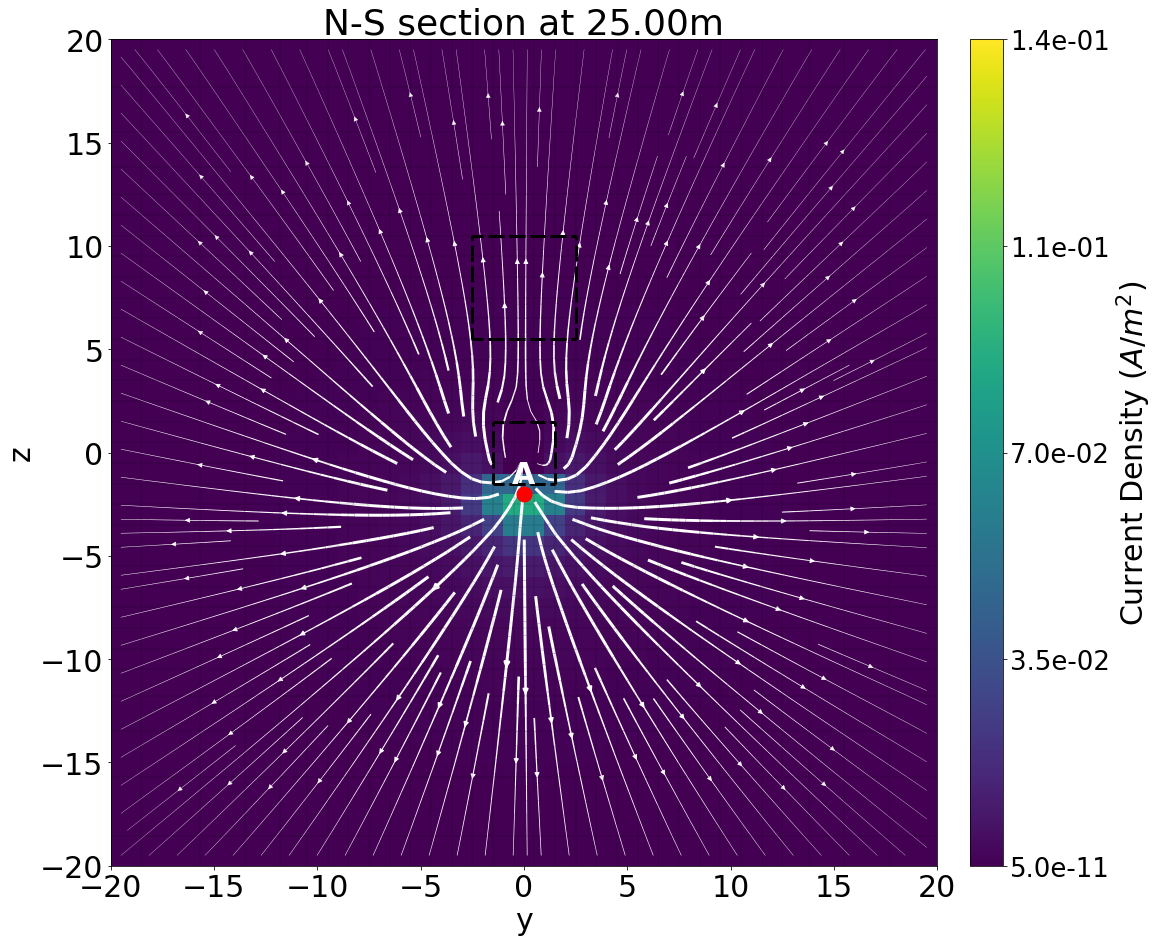
\includegraphics[trim=0cm 0cm 0cm 0cm, clip=true,width=\linewidth]{./Fig6b.png}
      \DIFaddendFL \end{subfigure}

      \begin{subfigure}{0.02\linewidth}
        \DIFdelbeginFL %DIFDELCMD < \begin{center}
%DIFDELCMD <             %%%
\DIFdelendFL \begin{turn}{90}
            \DIFdelbeginFL %DIFDELCMD < \scriptsize{\textbf{Secondary ($\vec{j_s}$)}}
%DIFDELCMD <             %%%
\DIFdelendFL \DIFaddbeginFL \begin{picture}(100,0)
                \put(65,0){\scriptsize{\textbf{Secondary ($\vec{j_s}$)}}}
            \end{picture}
        \DIFaddendFL \end{turn}
      \DIFdelbeginFL %DIFDELCMD < \end{center}
%DIFDELCMD <       %%%
\DIFdelendFL \end{subfigure}\hspace{-0.8cm}
      \qquad
      \begin{subfigure}{0.5\linewidth}
         \label{fig:Js_SingleLinearArray_Top_Blk5m_8mElecBlkCenter_3x3Tunnel_X3}
         \DIFdelbeginFL %DIFDELCMD < \sbox0{\includegraphics[trim=0cm 0cm 0cm 0cm, clip=true,width=\linewidth]{./Figures/TheoreticalAnalysis/Js_SingleLinearArray_Bottom_Blk5m_ZLocBlkCenter8m_3x3Tunnel_X=25.png}}
%DIFDELCMD <          \includegraphics[height=\ht0,keepaspectratio]{./Figures/TheoreticalAnalysis/Js_SingleLinearArray_Top_Blk5m_8mElecBlkCenter_3x3Tunnel_X=25_noCB.png}
%DIFDELCMD <       %%%
\DIFdelendFL \DIFaddbeginFL \sbox0{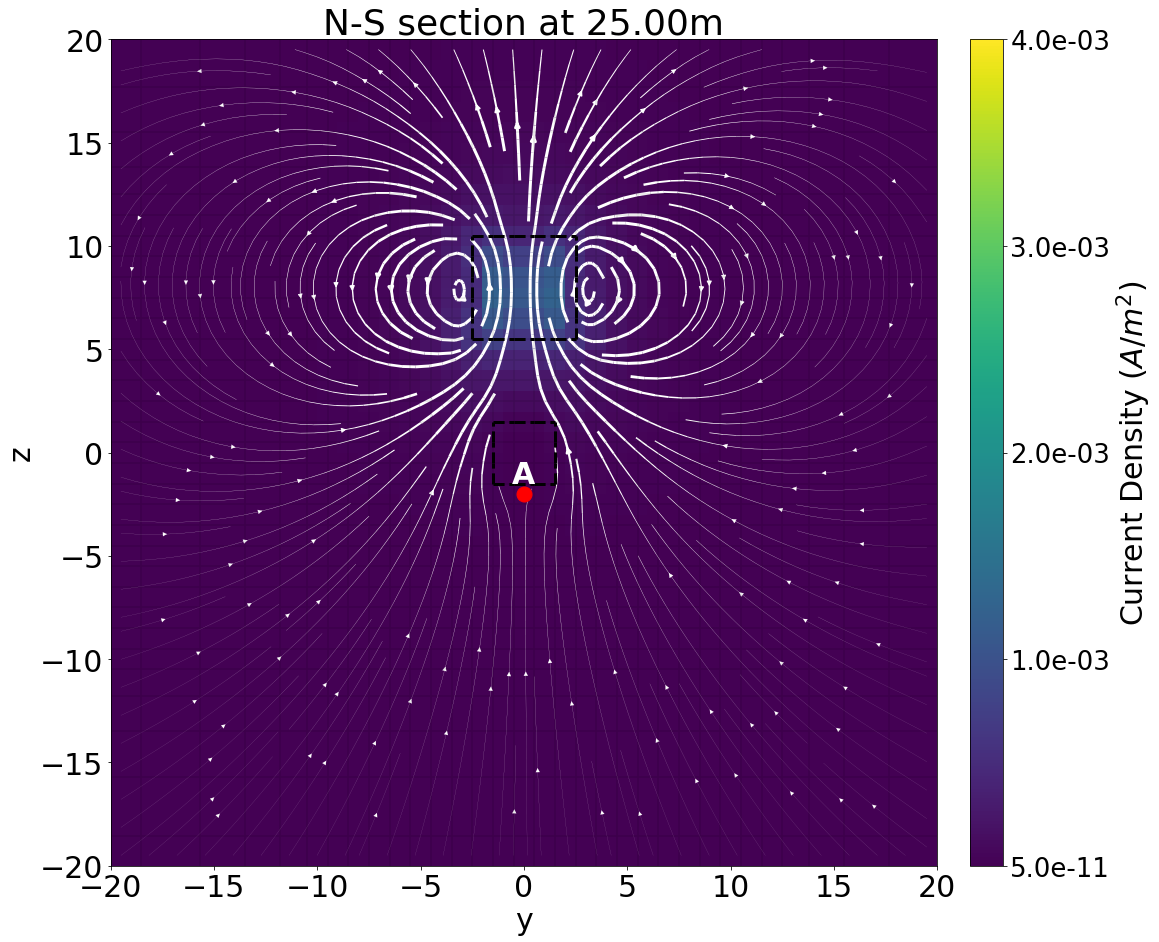
\includegraphics[trim=0cm 0cm 0cm 0cm, clip=true,width=\linewidth]{./Fig6d.png}}
         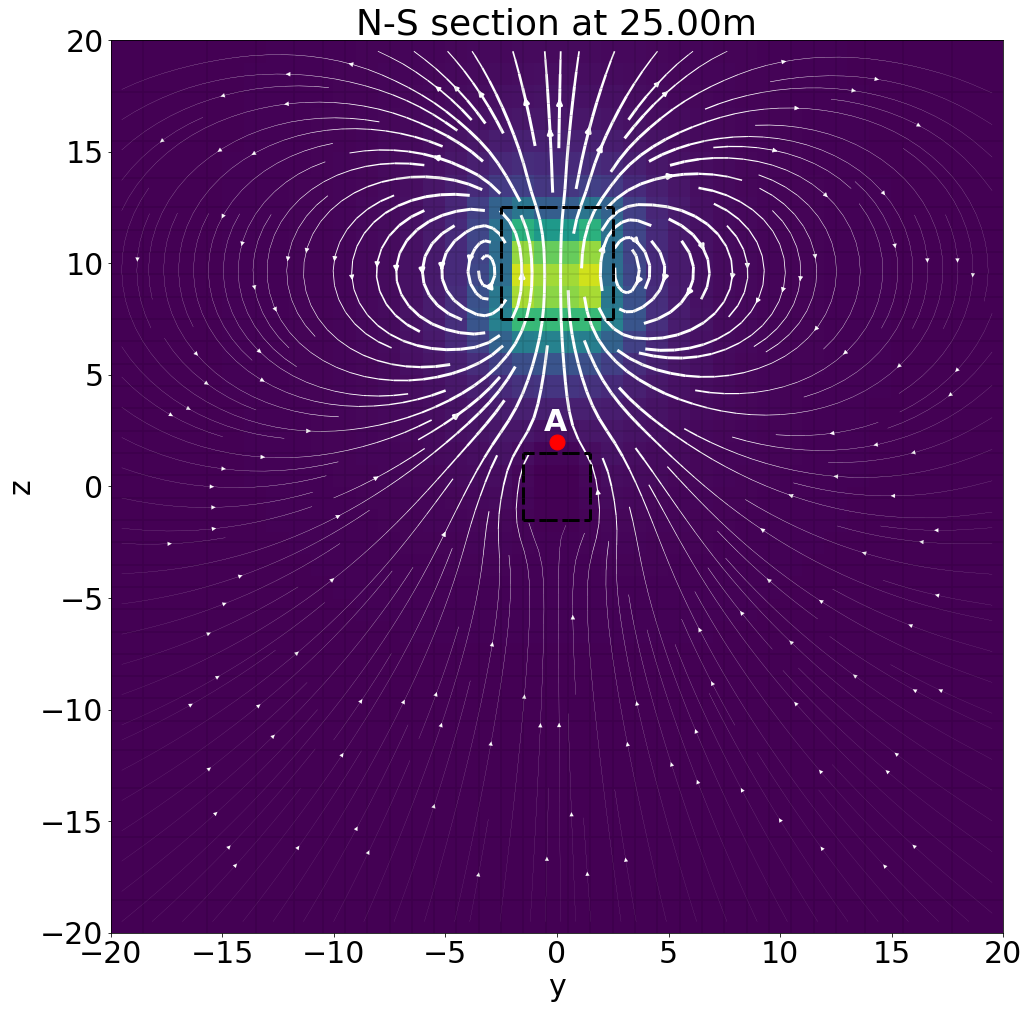
\includegraphics[height=\ht0,keepaspectratio]{./Fig6c.png}
      \DIFaddendFL \end{subfigure}\hspace{-0.9cm}
      %DIF <  \begin{subfigure}{0.5\linewidth}
      %DIF <     \label{fig:Js_SingleLinearArray_Side_Blk5m_8mElecBlkCenter_3x3Tunnel_X}
      %DIF <     \sbox0{\includegraphics[trim=0cm 0cm 0cm 0cm, clip=true,width=\linewidth]{./Figures/TheoreticalAnalysis/Js_SingleLinearArray_Side_Blk5m_8mElecBlkCenter_3x3Tunnel_X=25.png}}
      %DIF <     \includegraphics[height=\ht0,keepaspectratio]{./Figures/TheoreticalAnalysis/Js_SingleLinearArray_Side_Blk5m_8mElecBlkCenter_3x3Tunnel_X=25_noCB.png}
      %DIF <  \end{subfigure}\hspace{-0.9cm}
      \begin{subfigure}{0.5\linewidth}
         \label{fig:Js_SingleLinearArray_Bottom_Blk5m_ZLocBlkCenter8m_3x3Tunnel_X}
         \DIFdelbeginFL %DIFDELCMD < \includegraphics[trim=0cm 0cm 0cm 0cm, clip=true,width=\linewidth]{./Figures/TheoreticalAnalysis/Js_SingleLinearArray_Bottom_Blk5m_ZLocBlkCenter8m_3x3Tunnel_X=25.png}
%DIFDELCMD <       %%%
\DIFdelendFL \DIFaddbeginFL 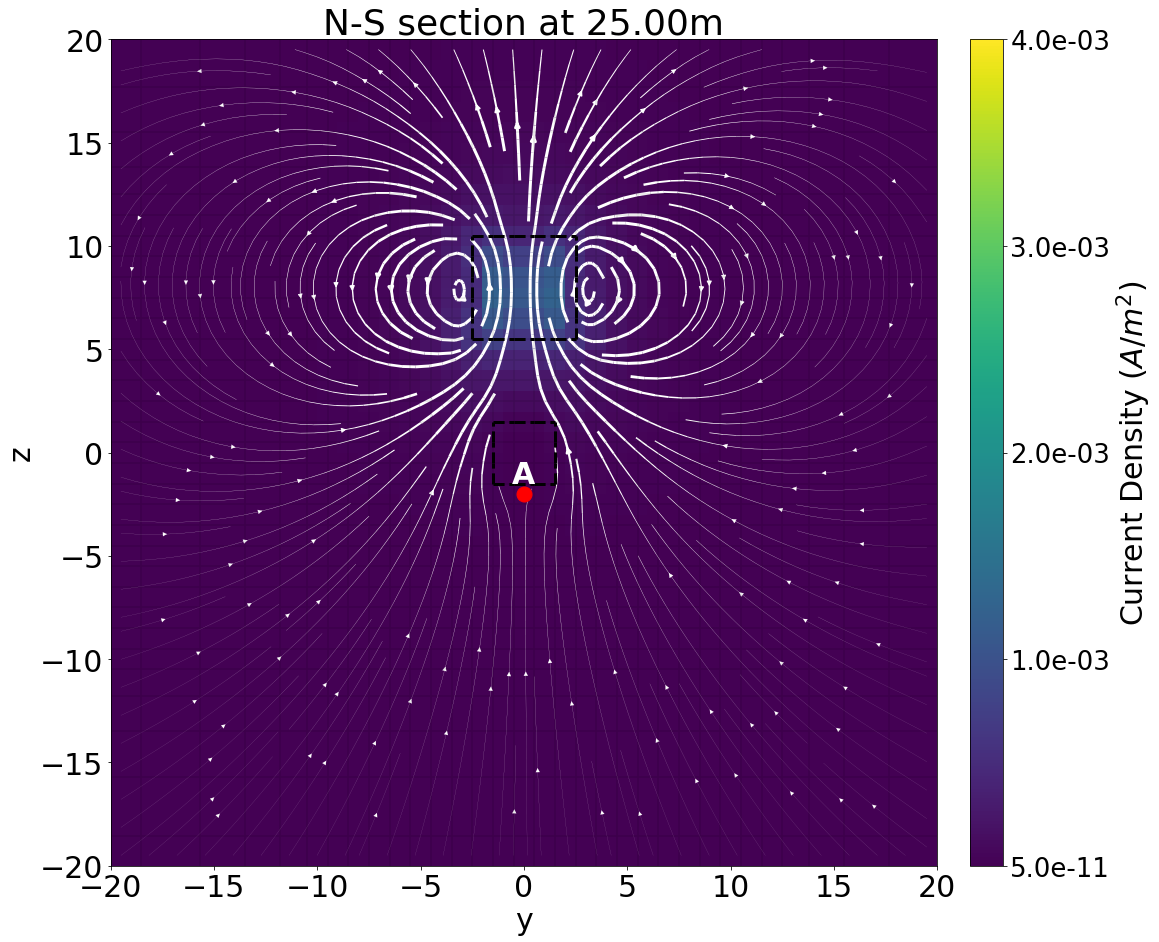
\includegraphics[trim=0cm 0cm 0cm 0cm, clip=true,width=\linewidth]{./Fig6d.png}
      \DIFaddendFL \end{subfigure}
   \DIFdelbeginFL %DIFDELCMD <

%DIFDELCMD <       %%%
%DIF <  \begin{subfigure}{0.02\linewidth}
      %DIF <     \begin{center}
      %DIF <        \begin{turn}{90}
      %DIF <              \scriptsize{\textbf{Total ($\vec{j_t}$)}}
      %DIF <        \end{turn}
      %DIF <     \end{center}
      %DIF <  \end{subfigure}\hspace{-0.8cm}
      %DIF <  \qquad
      %DIF <  \begin{subfigure}{0.5\linewidth}
      %DIF <     \label{fig:Jt_SingleLinearArray_Top_Blk5m_8mElecBlkCenter_3x3Tunnel_X3}
      %DIF <     \sbox0{\includegraphics[trim=0cm 0cm 0cm 0cm, clip=true,width=\linewidth]{./Figures/TheoreticalAnalysis/Jt_SingleLinearArray_Top_Blk5m_8mElecBlkCenter_3x3Tunnel_X=25.png}}
      %DIF <     \includegraphics[height=\ht0,keepaspectratio]{./Figures/TheoreticalAnalysis/Jt_SingleLinearArray_Top_Blk5m_8mElecBlkCenter_3x3Tunnel_X=25_noCB.png}
      %DIF <  \end{subfigure}\hspace{-0.9cm}
      %DIF <  \begin{subfigure}{0.5\linewidth}
      %DIF <     \label{fig:Jt_SingleLinearArray_Side_Blk5m_8mElecBlkCenter_3x3Tunnel_X}
      %DIF <     \sbox0{\includegraphics[trim=0cm 0cm 0cm 0cm, clip=true,width=\linewidth]{./Figures/TheoreticalAnalysis/Jt_SingleLinearArray_Side_Blk5m_8mElecBlkCenter_3x3Tunnel_X=25.png}}
      %DIF <     \includegraphics[height=\ht0,keepaspectratio]{./Figures/TheoreticalAnalysis/Jt_SingleLinearArray_Side_Blk5m_8mElecBlkCenter_3x3Tunnel_X=25_noCB.png}
      %DIF <  \end{subfigure}\hspace{-0.9cm}
      %DIF <  \begin{subfigure}{0.5\linewidth}
      %DIF <     \label{fig:Jt_SingleLinearArray_Bottom_Blk5m_ZLocBlkCenter8m_3x3Tunnel_X}
      %DIF <     \includegraphics[trim=0cm 0cm 0cm 0cm, clip=true,width=\linewidth]{./Figures/TheoreticalAnalysis/Jt_SingleLinearArray_Bottom_Blk5m_ZLocBlkCenter8m_3x3Tunnel_X=25.png}
      %DIF <  \end{subfigure}
   \DIFdelendFL \end{center}
\vspace{-0.4cm}
\caption{N-S sections showing variations in the primary and secondary current densities as the location of the pole TX (red dot) is moved to various sides of the 3 $\times$ 3 m tunnel. In the left column, the TX is on the tunnel ceiling and in the right column, the TX is on the floor of the tunnel. As in previous figures, the dashed black lines show the outlines of the conductive block and the E-W trending tunnel. \DIFaddbeginFL \DIFaddFL{The white arrows show current flow lines. }\DIFaddendFL As the TX is moved \DIFdelbeginFL \DIFdelFL{further }\DIFdelendFL \DIFaddbeginFL \DIFaddFL{farther }\DIFaddendFL around the tunnel, the primary current density in the vicinity of the conductive block decreases and the TX does a poorer job of exciting the target. In this way, the tunnel effectively shields the conductive block from the TX and reduces the magnitude of its secondary response.}
\label{fig:J_TunnelEffects_Top_Blk5m_3x3Tunnel_Elec_TopSideBottom}
\end{figure}

Although, in this configuration\DIFaddbegin \DIFadd{, }\DIFaddend the tunnel has broken the vertical symmetry, horizontal symmetry is retained \DIFdelbegin \DIFdel{. As }\DIFdelend \DIFaddbegin \DIFadd{as }\DIFaddend shown by the identical $\phi_{s}$ responses of blocks 1 and 3. For any location along the dashed circle there will be a second point mirrored about the $y$-axis that will produce an identical response. This \DIFaddbegin \DIFadd{configuration }\DIFaddend is analogous to the situation with a single offset TX in Trial 2 with the addition of current shielding effects.

\subsection{Summary of Non-Uniqueness and Resolution Analysis}
The results presented in this section show that in addition to having detectable differences in the data, TXs also need to be laid out symmetrically to create a uniform distribution of sensitivities about the array. To avoid inversion artifacts similar to those shown in Figure \ref{fig:SurveyDesign_SLA_Blk_8mSide_NoTunnel_OffsetTX_Trials_XZSections}, where conductive anomalies are incorrectly placed in regions with comparatively high sensitivity, the use of a ``ring'' of orthogonal electrodes is required. The shielding effect of the tunnel further accentuates sensitivity imbalances since the poorly excited regions on the opposite side of the tunnel from the TX have extremely low sensitivities. By placing one electrode in each face of the tunnel to form a ring of electrodes at each along-tunnel location\DIFaddbegin \DIFadd{, }\DIFaddend we can differentiate the response of conductive bodies at any location around the tunnel and uniformly distribute sensitivities.


%DIF <  \section{DC Resistivity Survey Design: Improving Model Resolution and Addressing Non-Uniqueness Issues}
%DIF <  \label{sec:SurveyDesign}
\section{Developing and Testing the Ring Array Survey}
\label{sec:RingArray_Development}

To address the model resolution and non-uniqueness issues discussed in the previous section\DIFaddbegin \DIFadd{, }\DIFaddend we propose the use of ring-shaped arrays of electrodes. Using a series of increasingly complex synthetic models we assess the benefits of ring arrays for designing surveys that better constrain the location and shape of anomalous bodies around the tunnel. Since ring arrays utilize far more electrodes than conventional linear arrays, we developed a physics-based survey design methodology that aids in the selection of a subset of TXs and RXs. In the proposed survey design methodology\DIFaddbegin \DIFadd{, }\DIFaddend TXs are selected based upon charge accumulation on a target test block\DIFaddbegin \DIFadd{, }\DIFaddend which is moved through the region of interest (ROI) and RXs are pseudo-randomly selected from a subset of measurements\DIFaddbegin \DIFadd{, }\DIFaddend which are sufficiently sensitive to the test block. We do not claim that this is a strictly optimal survey design \DIFdelbegin \DIFdel{, }\DIFdelend but show it to be a practical and computationally efficient way to balance improvements in model resolution with survey size.

\subsection{Selection of Base Survey Parameters}
\label{sec:RingArray_Development_BaseSurveyParams}

Before testing the ring array, appropriate base survey parameters need to be selected to ensure that anomalous bodies within the ROI are detectable. To perform this analysis we need to define the ROI, estimate the size of the target, and estimate the conductivity contrast between the target and background. With these estimates, forward modeling can be done to measure the response of different targets and determine which will be detectable. For a more detailed \DIFdelbegin \DIFdel{, }\DIFdelend discussion on detectability estimates see \citet{Mitchell2020}.

After some analysis of different array types, we determined that dipole-dipole measurements were best suited for this application since they had the highest near-tunnel sensitivities. \citet{Spitzer1998}, \citet{Dahlin2004}, and \citet{Okpoli2013} \DIFdelbegin \DIFdel{provide }\DIFdelend \DIFaddbegin \DIFadd{provided }\DIFaddend a good review of sensitivity variations and the resolution capacity of commonly used arrays. \DIFdelbegin \DIFdel{It should be noted that }\DIFdelend \DIFaddbegin \DIFadd{Here }\DIFaddend we use the term dipole-dipole generally to refer to any electrode configuration which utilizes a pair of electrodes for both the TX and RX. As a result, the comprehensive set of dipole-dipole configurations that are tested here incorporate all possible 4 electrode combinations and therefore include Wenner, Schlumberger, traditional dipole-dipole, gradient, and $\gamma$-array style measurements. All of these 4 electrode array types are found to have higher sensitivity and better resolution than pole-pole arrays \citep{Dahlin2004, Okpoli2013}. By combining measurements from each of these 4 electrode array types\DIFaddbegin \DIFadd{, }\DIFaddend we make use of the strengths of each individual array type to balance horizontal and vertical sensitivity to variations in conductivity and maximize resolution.

Selecting appropriate electrode separation distances is also important. For \DIFdelbegin \DIFdel{3D }\DIFdelend \DIFaddbegin \DIFadd{3-D }\DIFaddend surveys, having evenly spaced electrodes in each direction has been shown to improve the overall resolution of the recovered model \citep{Okpoli2013}. In the case of the ring array, this suggests that the along-tunnel or inter-ring separation distance should not be dramatically larger than the intra-ring spacing of electrodes. Since electrodes were placed in the center of each face of the 3 $\times$ 3 m tunnel at a distance of 2 m from the tunnel center, these synthetic trials have an intra-ring electrode spacing of 2.83 m. The electrodes were sunk half a cell into the tunnel wall to ensure that they are grounded and minimize numerical errors. An inter-ring spacing of 5 m along the length of the tunnel was found to produce far better inversion results than a 10 m inter-ring spacing. Figure \ref{fig:ElectrodeSpacing_StraightTunnel_Layout} illustrates the difference between intra-ring and inter-ring electrode separations. When the inter-ring spacing is considerably larger than the intra-ring spacing\DIFaddbegin \DIFadd{, }\DIFaddend it creates an imbalanced distribution of sensitivities, with much higher sensitivities around the tunnel at the ring locations than between the rings. This situation dramatically reduces the overall resolution of the survey and can cause inversion artifacts to be placed near the electrode rings or smeared from ring to ring.

\begin{figure}[htp]{}
\captionsetup[subfigure]{labelformat=empty}
   \begin{center}
      \begin{subfigure}{0.44\linewidth}
          \begin{picture}(100,0)
               \put(60,0){\scriptsize{\textbf{X Section}}}
         \end{picture}
      \end{subfigure}\hspace{-0.0cm}
      \qquad
      \begin{subfigure}{0.44\linewidth}
          \begin{picture}(100,0)
               \put(50,0){\scriptsize{\textbf{Y Section}}}
         \end{picture}
      \end{subfigure}\hspace{-0.0cm}

      \begin{subfigure}{0.56\linewidth}
         \label{fig:ElectrodeSpacing_StraightTunnel_Layout_Ring_X}
         \DIFdelbeginFL %DIFDELCMD < \sbox0{\includegraphics[trim=0cm 0cm 0cm 0cm, clip=true,width=\linewidth]{./Figures/SurveyDesign/TheoreticalAnalysis/TunnelEffects/Inter_Ring_StraightTunnel_SetupY=0_Ring.pdf}}
%DIFDELCMD <          \includegraphics[height=\ht0,keepaspectratio]{./Figures/SurveyDesign/TheoreticalAnalysis/TunnelEffects/Intra_Ring_StraightTunnel_SetupX=25_Ring.pdf}
%DIFDELCMD <       %%%
\DIFdelendFL \DIFaddbeginFL \sbox0{\includegraphics[trim=0cm 0cm 0cm 0cm, clip=true,width=\linewidth]{./Fig7b.pdf}}
         \includegraphics[height=\ht0,keepaspectratio]{./Fig7a.pdf}
      \DIFaddendFL \end{subfigure}
      \hspace{-2.5cm}
      % \hfill
      \begin{subfigure}{0.56\linewidth}
         \label{fig:ElectrodeSpacing_StraightTunnel_Layout_Ring_Y}
         \DIFdelbeginFL %DIFDELCMD < \includegraphics[trim=0cm 0cm 0cm 0cm, clip=true,width=\linewidth]{./Figures/SurveyDesign/TheoreticalAnalysis/TunnelEffects/Inter_Ring_StraightTunnel_SetupY=0_Ring.pdf}
%DIFDELCMD <       %%%
\DIFdelendFL \DIFaddbeginFL \includegraphics[trim=0cm 0cm 0cm 0cm, clip=true,width=\linewidth]{./Fig7b.pdf}
      \DIFaddendFL \end{subfigure}
   \end{center}
\vspace{-0.4cm}
\caption{Diagrams illustrating the difference between inter-ring and intra-ring electrode separation distances. Intra-ring separations measure the distance between electrodes within a single ring and inter-ring separations specify the distance between rings. The left column shows a N-S oriented section which perpendicularly cuts the tunnel, while the right column shows an E-W oriented section that parallels the tunnel. Electrode locations are marked by the black dots around the periphery of the blue \DIFdelbeginFL \DIFdelFL{$3 \times 3$ }\DIFdelendFL \DIFaddbeginFL \DIFaddFL{3 $\times$ 3 }\DIFaddendFL m tunnel.}
\label{fig:ElectrodeSpacing_StraightTunnel_Layout}
\end{figure}

When selecting inter-ring and intra-ring electrode separation distances\DIFaddbegin \DIFadd{, }\DIFaddend it is also important to take into account the estimated size of your target and the expected distance of the target from the tunnel/electrodes. A good rule of thumb is to select inter-ring and intra-ring electrode spacings similar to the larger of these two estimates. Since the sensitivity, and therefore the resolution of the array, decays rapidly \DIFdelbegin \DIFdel{as you move }\DIFdelend away from the electrodes\DIFaddbegin \DIFadd{, }\DIFaddend there is no reason to collect measurements using a very small electrode spacing if you expect the target to be far from the tunnel. These closely spaced measurements will help better constrain the near-tunnel region but will do little to improve the resolution of the distant target region. Conversely, trying to resolve a small target close to the tunnel with a large electrode spacing reduces sensitivity and resolution within the region of interest and can result in a missing or highly smeared anomaly in the recovered model.


%DIF <  \subsection{Testing and Developing the Ring Array Survey}
%DIF <  \label{sec:RingArray_Development}
\DIFdelbegin %DIFDELCMD <

%DIFDELCMD < %%%
%DIF <  The previous chapter showed how ring arrays can help address the fundamental non-uniqueness of the around-tunnel location of anomalous conductivity structures associated with the single linear array. we now need to evaluate the performance of the ring array and develop a way to design surveys using this electrode configuration. we begin with a discussion of how to select base survey parameters and then test the performance of the ring array on a series of increasingly complex synthetic models.
%DIFDELCMD <

%DIFDELCMD < %%%
\DIFdelend \subsubsection{Straight Tunnel Synthetics}
\label{sec:RingArray_Development_Straight_Synth_Intro}
The performance of the ring array was first tested on a series of models with conductive structures placed at various locations around a straight section of 3 $\times$ 3 m tunnel. In keeping with the previous modeling, a background conductivity of \DIFdelbegin \DIFdel{$5e-3$ }\DIFdelend \DIFaddbegin \DIFadd{$5 \times 10^{\text{-3}}$ }\DIFaddend S/m and a block conductivity of 10 S/m were used. With these models, we assess the ring arrays' ability to constrain the around-tunnel location of the target, the distance of the target away from the tunnel, and its ability to resolve more complex structures that mimic geology.

For each of these tests, we start simple and build up the complexity of the survey. Results are shown for a single linear array, 4 linear \DIFdelbegin \DIFdel{arrays}\DIFdelend \DIFaddbegin \DIFadd{array}\DIFaddend , and the ring array surveys. Diagrams showing orthogonal views of each survey layout are shown in Figure \ref{fig:SurveyDesign_StraightTunnel_Layout}. In these diagrams, the dashed lines denote the boundaries of the ROI which extends from \DIFdelbegin \DIFdel{$x=$}\DIFdelend \DIFaddbegin \DIFadd{$x$ = }\DIFaddend 15 m to \DIFdelbegin \DIFdel{$x=$}\DIFdelend \DIFaddbegin \DIFadd{$x$ = }\DIFaddend 35 m and from -20 \DIFdelbegin \DIFdel{m }\DIFdelend to 20 m in the $y$ and $z$-directions\DIFaddbegin \DIFadd{, respectively}\DIFaddend .

For the single linear array electrodes were placed at 5 m intervals from \DIFdelbegin \DIFdel{$x=$ }\DIFdelend \DIFaddbegin \DIFadd{$x$ = }\DIFaddend 0 to 50 m along the ceiling of the tunnel. In the 4 linear array survey, one of these 11 electrode linear arrays is laid along the center of each tunnel face. For each of the linear arrays, data are collected independently \DIFdelbegin \DIFdel{, }\DIFdelend (i.e.\DIFaddbegin \DIFadd{, }\DIFaddend all TX and RX electrodes were on the same face of the tunnel), but inverted collectively. For the ring array survey, rings of 4 electrodes with 1 electrode in the center of each face of the tunnel are placed at 5 m intervals within the central ROI and 10 m intervals outside of the ROI. For each of these surveys, all possible 4 electrode dipole-dipole measurements were included to form a comprehensive dataset. This caused the size of the survey to increase rapidly as the number of electrodes increased. Table \ref{table:SurveyDesign_FullSurveyStats} summarizes the size of each of these surveys.

\begin{table} [htp]
   %DIF <  \tiny, \scriptsize, \footnotesize,\small
   \footnotesize
    \begin{center}
        \begin{tabular}{| c | c | c | c |}
            \hline
             & \DIFdelbeginFL \DIFdelFL{\# Electrodes }\DIFdelendFL \DIFaddbeginFL \textbf{\DIFaddFL{\mbox{\boldmath$\#$} Electrodes}} \DIFaddendFL & \DIFdelbeginFL \DIFdelFL{\# TX }\DIFdelendFL \DIFaddbeginFL \textbf{\DIFaddFL{\mbox{\boldmath$\#$} TX}} \DIFaddendFL & \DIFdelbeginFL \DIFdelFL{\# Data}\DIFdelendFL \DIFaddbeginFL \textbf{\DIFaddFL{\mbox{\boldmath$\#$} Data}}\DIFaddendFL \\
            \hline
            Single Linear Array & 11 & 55 & 1,980 \\
            \hline
            Four Linear Arrays & 44 & 220 & 7,920 \\
            \hline
            Ring Array & 36 & 630 & 353,430 \\
            %DIF <  \hline
            %DIF <  Ring Array + Boreholes & 46 & 1,035 & 979,110 \\
            \hline
        \end{tabular}
    \end{center}
\caption{A table showing the size of each of the surveys tested in terms of the number of electrodes used, the number of TXs, and the total number of data.}
\label{table:SurveyDesign_FullSurveyStats}
\end{table}


\begin{figure}[htp]{}
\captionsetup[subfigure]{labelformat=empty}
   \begin{center}
      \begin{subfigure}{0.02\linewidth}
          % Blank Placeholder
      \end{subfigure}\hspace{-0.8cm}
      \qquad
      \begin{subfigure}{0.49\linewidth}
          \DIFdelbeginFL %DIFDELCMD < \begin{picture}(100,0)
%DIFDELCMD <                \put(45,0){\scriptsize{\textbf{X Section}}}
%DIFDELCMD <          \end{picture}
%DIFDELCMD <       %%%
\DIFdelendFL \DIFaddbeginFL \begin{picture}(100,0)
               \put(60,0){\scriptsize{\textbf{X Section}}}
         \end{picture}
      \DIFaddendFL \end{subfigure}\hspace{-0.8cm}
      \qquad
      \begin{subfigure}{0.49\linewidth}
          \DIFdelbeginFL %DIFDELCMD < \begin{picture}(100,0)
%DIFDELCMD <                \put(45,0){\scriptsize{\textbf{Y Section}}}
%DIFDELCMD <          \end{picture}
%DIFDELCMD <       %%%
\DIFdelendFL \DIFaddbeginFL \begin{picture}(100,0)
               \put(65,0){\scriptsize{\textbf{Y Section}}}
         \end{picture}
      \DIFaddendFL \end{subfigure}\hspace{-0.8cm}

      \vspace{0.1cm}
      \begin{subfigure}{0.02\linewidth}
         \DIFdelbeginFL %DIFDELCMD < \begin{center}
%DIFDELCMD <             %%%
\DIFdelendFL \begin{turn}{90}
            \DIFdelbeginFL %DIFDELCMD < \scriptsize{\textbf{Single Linear Array}}
%DIFDELCMD <             %%%
\DIFdelendFL \DIFaddbeginFL \begin{picture}(100,0)
                \put(34,0){\scriptsize{\textbf{Single Linear Array}}}
            \end{picture}
         \DIFaddendFL \end{turn}
      \DIFdelbeginFL %DIFDELCMD < \end{center}
%DIFDELCMD <       %%%
\DIFdelendFL \end{subfigure}\hspace{-0.8cm}
      \qquad
      \begin{subfigure}{0.49\linewidth}
         \label{fig:SurveyDesign_StraightTunnel_Layout_SingleLinearArray_X}
         \DIFdelbeginFL %DIFDELCMD < \sbox0{\includegraphics[trim=0cm 0cm 0cm 0cm, clip=true,width=\linewidth]{./Figures/SurveyDesign/TheoreticalAnalysis/TunnelEffects/StraightTunnel_SetupY=0_SingleLinearArray.pdf}}
%DIFDELCMD <          \includegraphics[height=\ht0,keepaspectratio]{./Figures/SurveyDesign/TheoreticalAnalysis/TunnelEffects/StraightTunnel_SetupX=25_SingleLinearArray.pdf}
%DIFDELCMD <       %%%
\DIFdelendFL \DIFaddbeginFL \sbox0{\includegraphics[trim=0cm 0cm 0cm 0cm, clip=true,width=\linewidth]{./Fig8b.pdf}}
         \includegraphics[height=\ht0,keepaspectratio]{./Fig8a.pdf}
      \DIFaddendFL \end{subfigure}\hspace{-0.9cm}
      \begin{subfigure}{0.49\linewidth}
         \label{fig:SurveyDesign_StraightTunnel_Layout_SingleLinearArray_Y}
         \DIFdelbeginFL %DIFDELCMD < \includegraphics[trim=0cm 0cm 0cm 0cm, clip=true,width=\linewidth]{./Figures/SurveyDesign/TheoreticalAnalysis/TunnelEffects/StraightTunnel_SetupY=0_SingleLinearArray.pdf}
%DIFDELCMD <       %%%
\DIFdelendFL \DIFaddbeginFL \includegraphics[trim=0cm 0cm 0cm 0cm, clip=true,width=\linewidth]{./Fig8b.pdf}
      \DIFaddendFL \end{subfigure}

      \begin{subfigure}{0.02\linewidth}
         \DIFdelbeginFL %DIFDELCMD < \begin{center}
%DIFDELCMD <             %%%
\DIFdelendFL \begin{turn}{90}
            \DIFdelbeginFL %DIFDELCMD < \scriptsize{\textbf{4 Linear Arrays}}
%DIFDELCMD <             %%%
\DIFdelendFL \DIFaddbeginFL \begin{picture}(100,0)
                \put(46,0){\scriptsize{\textbf{4 Linear Array}}}
            \end{picture}
         \DIFaddendFL \end{turn}
      \DIFdelbeginFL %DIFDELCMD < \end{center}
%DIFDELCMD <       %%%
\DIFdelendFL \end{subfigure}\hspace{-0.8cm}
      \qquad
      \begin{subfigure}{0.49\linewidth}
         \label{fig:SurveyDesign_StraightTunnel_Layout_4LinearArrays_X}
         \DIFdelbeginFL %DIFDELCMD < \sbox0{\includegraphics[trim=0cm 0cm 0cm 0cm, clip=true,width=\linewidth]{./Figures/SurveyDesign/TheoreticalAnalysis/TunnelEffects/StraightTunnel_SetupY=0_4LinearArrays.pdf}}
%DIFDELCMD <          \includegraphics[height=\ht0,keepaspectratio]{./Figures/SurveyDesign/TheoreticalAnalysis/TunnelEffects/StraightTunnel_SetupX=25_4LinearArrays.pdf}
%DIFDELCMD <       %%%
\DIFdelendFL \DIFaddbeginFL \sbox0{\includegraphics[trim=0cm 0cm 0cm 0cm, clip=true,width=\linewidth]{./Fig8d.pdf}}
         \includegraphics[height=\ht0,keepaspectratio]{./Fig8c.pdf}
      \DIFaddendFL \end{subfigure}\hspace{-0.9cm}
      \begin{subfigure}{0.49\linewidth}
         \label{fig:SurveyDesign_StraightTunnel_Layout_4LinearArrays_Y}
         \DIFdelbeginFL %DIFDELCMD < \includegraphics[trim=0cm 0cm 0cm 0cm, clip=true,width=\linewidth]{./Figures/SurveyDesign/TheoreticalAnalysis/TunnelEffects/StraightTunnel_SetupY=0_4LinearArrays.pdf}
%DIFDELCMD <       %%%
\DIFdelendFL \DIFaddbeginFL \includegraphics[trim=0cm 0cm 0cm 0cm, clip=true,width=\linewidth]{./Fig8d.pdf}
      \DIFaddendFL \end{subfigure}

      \begin{subfigure}{0.02\linewidth}
          \DIFdelbeginFL %DIFDELCMD < \begin{center}
%DIFDELCMD <             %%%
\DIFdelendFL \begin{turn}{90}
            \DIFdelbeginFL %DIFDELCMD < \scriptsize{\textbf{Ring Array}}
%DIFDELCMD <             %%%
\DIFdelendFL \DIFaddbeginFL \begin{picture}(100,0)
                \put(54,0){\scriptsize{\textbf{Ring Array}}}
            \end{picture}
          \DIFaddendFL \end{turn}
      \DIFdelbeginFL %DIFDELCMD < \end{center}
%DIFDELCMD <       %%%
\DIFdelendFL \end{subfigure}\hspace{-0.8cm}
      \qquad
      \begin{subfigure}{0.49\linewidth}
         \label{fig:SurveyDesign_StraightTunnel_Layout_Ring_X}
         \DIFdelbeginFL %DIFDELCMD < \sbox0{\includegraphics[trim=0cm 0cm 0cm 0cm, clip=true,width=\linewidth]{./Figures/SurveyDesign/TheoreticalAnalysis/TunnelEffects/StraightTunnel_SetupY=0_Ring.pdf}}
%DIFDELCMD <          \includegraphics[height=\ht0,keepaspectratio]{./Figures/SurveyDesign/TheoreticalAnalysis/TunnelEffects/StraightTunnel_SetupX=25_Ring.pdf}
%DIFDELCMD <       %%%
\DIFdelendFL \DIFaddbeginFL \sbox0{\includegraphics[trim=0cm 0cm 0cm 0cm, clip=true,width=\linewidth]{./Fig8f.pdf}}
         \includegraphics[height=\ht0,keepaspectratio]{./Fig8e.pdf}
      \DIFaddendFL \end{subfigure}\hspace{-0.9cm}
      \begin{subfigure}{0.49\linewidth}
         \label{fig:SurveyDesign_StraightTunnel_Layout_Ring_Y}
         \DIFdelbeginFL %DIFDELCMD < \includegraphics[trim=0cm 0cm 0cm 0cm, clip=true,width=\linewidth]{./Figures/SurveyDesign/TheoreticalAnalysis/TunnelEffects/StraightTunnel_SetupY=0_Ring.pdf}
%DIFDELCMD <       %%%
\DIFdelendFL \DIFaddbeginFL \includegraphics[trim=0cm 0cm 0cm 0cm, clip=true,width=\linewidth]{./Fig8f.pdf}
      \DIFaddendFL \end{subfigure}
   \DIFdelbeginFL %DIFDELCMD <

%DIFDELCMD <       %%%
%DIF <  \begin{subfigure}{0.02\linewidth}
      %DIF <     \begin{center}
      %DIF <        \begin{turn}{90}
      %DIF <              \scriptsize{\textbf{Ring Array + Boreholes}}
      %DIF <        \end{turn}
      %DIF <     \end{center}
      %DIF <  \end{subfigure}\hspace{-0.8cm}
      %DIF <  \qquad
      %DIF <  \begin{subfigure}{0.39\linewidth}
      %DIF <     \label{fig:SurveyDesign_StraightTunnel_Layout_Ring_BoreDiag1_X}
      %DIF <     \sbox0{\includegraphics[trim=0cm 0cm 0cm 0cm, clip=true,width=\linewidth]{./Figures/SurveyDesign/TheoreticalAnalysis/TunnelEffects/StraightTunnel_SetupY=0_Ring_BoreDiag1.pdf}}
      %DIF <     \includegraphics[height=\ht0,keepaspectratio]{./Figures/SurveyDesign/TheoreticalAnalysis/TunnelEffects/StraightTunnel_SetupX=25_Ring_BoreDiag1.pdf}
      %DIF <  \end{subfigure}\hspace{-0.9cm}
      %DIF <  \begin{subfigure}{0.39\linewidth}
      %DIF <     \label{fig:SurveyDesign_StraightTunnel_Layout_Ring_BoreDiag1_Y}
      %DIF <     \includegraphics[trim=0cm 0cm 0cm 0cm, clip=true,width=\linewidth]{./Figures/SurveyDesign/TheoreticalAnalysis/TunnelEffects/StraightTunnel_SetupY=0_Ring_BoreDiag1.pdf}
      %DIF <  \end{subfigure}
   \DIFdelendFL \end{center}
\vspace{-0.4cm}
\caption{A series of diagrams showing orthogonal views of each survey layout. The left column shows N-S oriented sections which perpendicularly cut the tunnel, while the right column shows E-W oriented sections that parallel the tunnel. Each row of figures shows the changes in electrode placement as the complexity of the survey increases from the single linear array (top) to the ring array survey (bottom). The dashed lines mark the boundaries of the region of interest (ROI) around the tunnel. Electrode locations are marked by the black dots around the tunnel periphery.}
\label{fig:SurveyDesign_StraightTunnel_Layout}
\end{figure}


%DIF <  Before completing the inversion trials to test the performance of these different surveys we first need to assess their ability to detect a conductive target. As done in Section \ref{sec:RingArray_Development_BaseSurveyParams} we forward modeled data for a range of block sizes and block offset distances for each survey. The mean $SNR_{s}$ for each dataset was then computed assuming $1\%$ noise plus a $1e-5$ V/A floor. As discussed in Section \ref{sec:RingArray_Development_BaseSurveyParams} the mean $SNR_{s}$ contours can be used to estimate the detectability of a given target. To be detectable, the mean $SNR_{s}$ must be larger than the estimated noise level of the dataset.
\DIFdelbegin %DIFDELCMD <

%DIFDELCMD < %%%
%DIF <  \begin{figure}[htp]{}
%DIF <  \captionsetup[subfigure]{}
%DIF <     \begin{center}
%DIF <        \begin{subfigure}{0.5\linewidth}
%DIF <           \label{fig:normMeanMisfit_BlkSizeVsSepDist_SingleLinearArray_DpDp_3x3Tunnel}
%DIF <           \sbox0{\includegraphics[trim=0cm 0cm 0cm 0cm, clip=true,width=\linewidth]{./Figures/SurveyDesign/TheoreticalAnalysis/TunnelEffects/normMisfitMean_BlkSizeVsSepDist_SingleLinearArray_DpDp_3x3Tunnel_log.pdf}}
%DIF <           \includegraphics[height=\ht0,keepaspectratio]{./Figures/SurveyDesign/TheoreticalAnalysis/TunnelEffects/normMisfitMean_BlkSizeVsSepDist_SingleLinearArray_DpDp_3x3Tunnel_log_noCB.pdf}
%DIF <           \caption{Single Linear Array}
%DIF <        \end{subfigure}\hspace{-0.9cm}
%DIF <        \begin{subfigure}{0.5\linewidth}
%DIF <           \label{fig:normMeanMisfit_BlkSizeVsSepDist_4LinearArrays_DpDp_3x3Tunnel}
%DIF <           \includegraphics[trim=0cm 0cm 0cm 0cm, clip=true,width=\linewidth]{./Figures/SurveyDesign/TheoreticalAnalysis/TunnelEffects/normMisfitMean_BlkSizeVsSepDist_4LinearArrays_DpDp_3x3Tunnel_log.pdf}
%DIF <           \caption{4 Linear Arrays}
%DIF <        \end{subfigure}
%DIF <        \qquad
%DIF <        \begin{subfigure}{0.5\linewidth}
%DIF <           \label{fig:normMeanMisfit_BlkSizeVsSepDist_Ring_DpDp_3x3Tunnel}
%DIF <           \sbox0{\includegraphics[trim=0cm 0cm 0cm 0cm, clip=true,width=\linewidth]{./Figures/SurveyDesign/TheoreticalAnalysis/TunnelEffects/normMisfitMean_BlkSizeVsSepDist_Ring_CenterROI_5mSep_DpDp_3x3Tunnel_log.pdf}}
%DIF <           \includegraphics[height=\ht0,keepaspectratio]{./Figures/SurveyDesign/TheoreticalAnalysis/TunnelEffects/normMisfitMean_BlkSizeVsSepDist_Ring_CenterROI_5mSep_DpDp_3x3Tunnel_log_noCB.pdf}
%DIF <           \caption{Ring Array}
%DIF <        \end{subfigure}\hspace{-0.9cm}
%DIF <        \begin{subfigure}{0.5\linewidth}
%DIF <           \label{fig:normMeanMisfit_BlkSizeVsSepDist_Ring_BoreDiag1_DpDp_3x3Tunnel}
%DIF <           \includegraphics[trim=0cm 0cm 0cm 0cm, clip=true,width=\linewidth]{./Figures/SurveyDesign/TheoreticalAnalysis/TunnelEffects/normMisfitMean_BlkSizeVsSepDist_Ring_CenterROI_5mSep_BoreDiag1_DpDp_3x3Tunnel_log.pdf}
%DIF <           \caption{Ring Array + Boreholes}
%DIF <        \end{subfigure}
%DIF <     \end{center}
%DIF <  \vspace{-0.4cm}
%DIF <  \caption{A series of contour plots which shows how the detectability of the conductive block varies for each of the surveys as the size of the block and its distance above the electrodes are varied. Here the mean $SNR_{s}$ (mean $|\phi_{s}/\xi|$) is used as the detectability metric. Each plot shows an increase in the complexity of the survey design from a single linear array to the ring array plus boreholes.}
%DIF <  \label{fig:SurveyDesign_StraightTunnel_Layout_BlkSizeVsSepDist_SurveyComp}
%DIF <  \end{figure}
%DIFDELCMD <

%DIFDELCMD < %%%
%DIF <  Figure \ref{fig:SurveyDesign_StraightTunnel_Layout_BlkSizeVsSepDist_SurveyComp} contains contour plots of the computed signal-to-noise ratios which clearly show an increase in detectability for the ring based arrays over the linear arrays (see Figure \ref{fig:SurveyDesign_StraightTunnel_Layout_BlkSizeVsSepDist_SurveyComp}). This is shown by the fact that for a given block size and offset the ring array has higher mean $SNR_{s}$ than the single linear array. The higher misfits cause the same sized block to be detectable out to larger offsets with the ring array. For example, if a noise level of $1\%$ plus a $1e-5$ V/A floor is assumed, the 5 m block is detectable out to an offset of 8 m for the single linear array and out to 10 m for the ring array.
%DIFDELCMD <

%DIFDELCMD < %%%
%DIF <  For the 4 linear array survey, a decrease in the mean $SNR_{s}$ is observed compared to the single linear array survey since the arrays on the walls and floor of the tunnel are not very sensitive to the conductive block above the tunnel. Due to their lack of sensitivity to the block, many of the additional data have very small secondary responses that are easily fit by the background model. These small secondary responses produce low $SNR_{s}$ which bring down the mean.
%DIFDELCMD <

%DIFDELCMD < %%%
%DIF <  The addition of the off-tunnel boreholes to the ring array significantly improves our ability to detect blocks with large offset distances. Assuming a noise level of $1\%$ plus a $1e-5$ V/A floor then at an offset distance of 18.5 m the conductive target needs to be larger than the 9 m cube to be detectable with the ring array plus boreholes survey. At the same offset distance, the target would have to be larger than an 11 m cube to be detectable using the ring array survey and larger than a 15 m cube to be detectable with the single linear array survey. This indicates that at an offset distance of 18.5 m the ring array plus borehole survey is capable of detecting a conductive target which is almost half the size of the smallest target which is detectable using the single linear array survey.
%DIFDELCMD <

%DIFDELCMD < %%%
%DIF <  Since the results of this detectability analysis show that the ring array produces a quantifiable increase in the secondary response of a conductive target we can now test the performance of each survey through inversion. In addition to improving the detectability of near-tunnel targets the ring array also dramatically increases the number of data and provides a more uniform distribution of sensitivities around the tunnel. All of these factors should help to better constrain anomalies within the recovered model by improving resolution and reducing non-uniqueness. These results also guide the creation of the synthetic models because they help estimate the detectable size and offset distance of targets. Having chosen to use a 5 m conductive block in the following tests, these plots show that with a $2\%$ noise level a maximum 7 m offset distance from the tunnel should be used to ensure that the target remains detectable.
%DIFDELCMD <

%DIFDELCMD < %%%
\DIFdelend \subsubsection{Around-Tunnel Location of the Target}
\label{sec:RingArray_Development_Straight_Synth_AroundTunnel}

To characterize the ability of each survey to constrain the around-tunnel location of the target\DIFaddbegin \DIFadd{, }\DIFaddend we placed a 5 m conductive cube 3 m away from the southern wall of the tunnel. As in previous examples, the conductive block has a conductivity of 10 S/m and the background conductivity is \DIFdelbegin \DIFdel{$5e-3$ }\DIFdelend \DIFaddbegin \DIFadd{$5 \times 10^{\text{-3}}$ }\DIFaddend S/m. Using SimPEG, synthetic data \DIFdelbegin \DIFdel{was }\DIFdelend \DIFaddbegin \DIFadd{were }\DIFaddend forward modeled for each survey, contaminated with 2$\%$ Gaussian noise \DIFdelbegin \DIFdel{, }\DIFdelend \DIFaddbegin \DIFadd{(i.e., randomly sampled noise from a normal distribution which varies from 0 to 2$\%$ of each measurement), }\DIFaddend and inverted. The results of these inversions show that our ability to constrain the around-tunnel location of the conductive block improves substantially as the survey is built up from the single linear array to the ring array (see Figure \ref{fig:SurveyDesign_StraightTunnel_3mSide_XZSections}).

Although the single linear array helps determine the along-tunnel location of the block, it does a very poor job of constraining its around-tunnel location. The recovered anomaly forms a conductive ring centered about the electrodes in the center of the tunnel ceiling, instead of its true location on the southern side of the tunnel. This conductive ring-like artifact is a result of the single linear array's inherent non-uniqueness in constraining the around-tunnel location of anomalies as discussed in Section \ref{sec:Resolution_&_NonUniqueness} and its highly asymmetric distribution of sensitivities. With the 4 linear array survey, the recovered anomaly is now located on the correct side of the tunnel and is spherical \DIFdelbegin \DIFdel{, }\DIFdelend but underestimates the distance of the block from the tunnel. The recovered model continues to improve with the introduction of the ring array. The conductive anomaly has now pulled away from the tunnel and moved closer to its true location on the south side of the tunnel. With the ring array, the recovered anomaly is also more compact and has a higher conductivity contrast with the background.


%DIF <  With the addition of off-tunnel boreholes, we can better constrain the distance of the block away from the tunnel but the overall changes in the recovered model are minor. This is because the block is close to the tunnel in this example and the ring array measurements do a good job of constraining its location. The off-tunnel boreholes will likely provide greater benefit for resolving more complex structures and targets located further away from the tunnel.
\DIFdelbegin %DIFDELCMD <

%DIFDELCMD < %%%
\DIFdelend \begin{figure}[htp]{}
\captionsetup[subfigure]{labelformat=empty}
   \begin{center}
      %DIF <  \begin{subfigure}{0.02\linewidth}
      %DIF <      % Blank Placeholder
      %DIF <  \end{subfigure}\hspace{-0.8cm}
      %DIF <  \qquad
      %DIF <  \begin{subfigure}{0.44\linewidth}
      %DIF <      \begin{picture}(100,0)
      %DIF <           \put(56,0){\scriptsize{\textbf{X Section}}}
      %DIF <     \end{picture}
      %DIF <  \end{subfigure}\hspace{-0.8cm}
      %DIF <  \qquad
      %DIF <  \begin{subfigure}{0.44\linewidth}
      %DIF <      \begin{picture}(100,0)
      %DIF <           \put(52,0){\scriptsize{\textbf{Z Section}}}
      %DIF <     \end{picture}
      %DIF <  \end{subfigure}\hspace{-0.8cm}
\DIFdelbeginFL %DIFDELCMD <

%DIFDELCMD <       %%%
\DIFdelendFL \vspace{0.1cm}
      \begin{subfigure}{0.02\linewidth}
         \DIFdelbeginFL %DIFDELCMD < \begin{center}
%DIFDELCMD <             %%%
\DIFdelendFL \begin{turn}{90}
            \DIFdelbeginFL %DIFDELCMD < \scriptsize{\textbf{Single Linear Array}}
%DIFDELCMD <             %%%
\DIFdelendFL \DIFaddbeginFL \begin{picture}(100,0)
                \put(30,0){\scriptsize{\textbf{Single Linear Array}}}
            \end{picture}
         \DIFaddendFL \end{turn}
      \DIFdelbeginFL %DIFDELCMD < \end{center}
%DIFDELCMD <       %%%
\DIFdelendFL \end{subfigure}\hspace{-0.8cm}
      \qquad
      \begin{subfigure}{0.845\linewidth}
         \label{fig:SurveyDesign_StraightTunnel_3mSide_SingleLinearArray_XZ}
         \DIFdelbeginFL %DIFDELCMD < \includegraphics[trim=0cm 0cm 0cm 0cm, clip=true,width=\linewidth]{./Figures/SurveyDesign/SingleLinearArray/InvMod_Sections_SingleLinearArray_5mSep_DC_Single5mBlk_3mSide_XZ.pdf}
%DIFDELCMD <       %%%
\DIFdelendFL \DIFaddbeginFL \includegraphics[trim=0cm 0cm 0cm 0cm, clip=true,width=\linewidth]{./Fig9a.pdf}
      \DIFaddendFL \end{subfigure}

      \begin{subfigure}{0.02\linewidth}
         \DIFdelbeginFL %DIFDELCMD < \begin{center}
%DIFDELCMD <             %%%
\DIFdelendFL \begin{turn}{90}
            \DIFdelbeginFL %DIFDELCMD < \scriptsize{\textbf{4 Linear Arrays}}
%DIFDELCMD <             %%%
\DIFdelendFL \DIFaddbeginFL \begin{picture}(100,0)
                \put(42,0){\scriptsize{\textbf{4 Linear Array}}}
            \end{picture}
         \DIFaddendFL \end{turn}
      \DIFdelbeginFL %DIFDELCMD < \end{center}
%DIFDELCMD <       %%%
\DIFdelendFL \end{subfigure}\hspace{-0.8cm}
      \qquad
      \begin{subfigure}{0.845\linewidth}
         \label{fig:SurveyDesign_StraightTunnel_3mSide_4LinearArrays_XZ}
         \DIFdelbeginFL %DIFDELCMD < \includegraphics[trim=0cm 0cm 0cm 0cm, clip=true,width=\linewidth]{./Figures/SurveyDesign/4LinearArrays/InvMod_Sections_4LinearArrays_5mSep_DC_Single5mBlk_3mSide_XZ.pdf}
%DIFDELCMD <       %%%
\DIFdelendFL \DIFaddbeginFL \includegraphics[trim=0cm 0cm 0cm 0cm, clip=true,width=\linewidth]{./Fig9b.pdf}
      \DIFaddendFL \end{subfigure}

      \begin{subfigure}{0.02\linewidth}
         \DIFdelbeginFL %DIFDELCMD < \begin{center}
%DIFDELCMD <             %%%
\DIFdelendFL \begin{turn}{90}
            \DIFdelbeginFL %DIFDELCMD < \scriptsize{\textbf{Ring Array}}
%DIFDELCMD <             %%%
\DIFdelendFL \DIFaddbeginFL \begin{picture}(100,0)
                \put(48,0){\scriptsize{\textbf{Ring Array}}}
            \end{picture}
         \DIFaddendFL \end{turn}
      \DIFdelbeginFL %DIFDELCMD < \end{center}
%DIFDELCMD <       %%%
\DIFdelendFL \end{subfigure}\hspace{-0.8cm}
      \qquad
      \begin{subfigure}{0.845\linewidth}
         \label{fig:SurveyDesign_StraightTunnel_3mSide_Ring_XZ}
         \DIFdelbeginFL %DIFDELCMD < \includegraphics[trim=0cm 0cm 0cm 0cm, clip=true,width=\linewidth]{./Figures/SurveyDesign/RingArrays/InvMod_Sections_RingArrayFull_5mSep_DC_Single5mBlk_3mSide_XZ.pdf}
%DIFDELCMD <       %%%
\DIFdelendFL \DIFaddbeginFL \includegraphics[trim=0cm 0cm 0cm 0cm, clip=true,width=\linewidth]{./Fig9c.pdf}
      \DIFaddendFL \end{subfigure}
   \DIFdelbeginFL %DIFDELCMD <

%DIFDELCMD <       %%%
%DIF <  \begin{subfigure}{0.02\linewidth}
      %DIF <     \begin{center}
      %DIF <        \begin{turn}{90}
      %DIF <              \scriptsize{\textbf{Ring Array + Boreholes}}
      %DIF <        \end{turn}
      %DIF <     \end{center}
      %DIF <  \end{subfigure}\hspace{-0.8cm}
      %DIF <  \qquad
      %DIF <  \begin{subfigure}{0.845\linewidth}
      %DIF <     \label{fig:SurveyDesign_StraightTunnel_3mSide_Ring_BoreDiag1_XZ}
      %DIF <     \includegraphics[trim=0cm 0cm 0cm 0cm, clip=true,width=\linewidth]{./Figures/SurveyDesign/RingArrays/InvMod_Sections_RingBore1_Full_5mSep_DC_Single5mBlk_3mSide_XZ.pdf}
      %DIF <  \end{subfigure}
   \DIFdelendFL \end{center}
\vspace{-0.4cm}
\caption{$x$ and $z$ sections through the recovered models show how our ability to constrain the location of a conductive block off to the side of the tunnel incrementally improves with the different survey designs. The white dots are projections of the electrode locations onto the section\DIFaddbeginFL \DIFaddFL{, the tunnel cells are dark purple, }\DIFaddendFL and the black dashed outlines show the edges of structures in the true model.}
\label{fig:SurveyDesign_StraightTunnel_3mSide_XZSections}
\end{figure}


\subsubsection{Resolving Multiple Blocks}
\label{sec:RingArray_Development_Straight_Synth_MultiBlk}

We then increased the complexity of the model by adding several conductive blocks at various locations around the tunnel. Figure \ref{fig:StraightTunnel_MultiBlk_TrueMod} shows two \DIFdelbegin \DIFdel{3D }\DIFdelend \DIFaddbegin \DIFadd{3-D }\DIFaddend views of the true multiple block model with the blocks labeled 1-3 for ease of reference. In keeping with the previous trials, the blocks were assigned a conductivity of 10 S/m in contrast to the \DIFdelbegin \DIFdel{$5e-3$ }\DIFdelend \DIFaddbegin \DIFadd{$5 \times 10^{\text{-3}}$ }\DIFaddend S/m background.

\begin{figure}[htp]{}
   \begin{center}
      \begin{subfigure}{0.54\linewidth}
         \DIFdelbeginFL %DIFDELCMD < \sbox0{\includegraphics[trim=0cm 0cm 0cm 0cm, clip=true,width=\linewidth]{./Figures/SurveyDesign/MultiBlk_TrueMod_Top_Crop.png}}
%DIFDELCMD <          \includegraphics[height=\ht0,keepaspectratio]{./Figures/SurveyDesign/MultiBlk_TrueMod_West_Crop.png}
%DIFDELCMD <          %%%
\DIFdelendFL \DIFaddbeginFL \sbox0{\includegraphics[trim=0cm 0cm 0cm 0cm, clip=true,width=\linewidth]{./Fig10b.png}}
         \includegraphics[height=\ht0,keepaspectratio]{./Fig10a.png}
         \DIFaddendFL \caption{West View}
         \label{fig:StraightTunnel_MultiBlk_TrueMod_West}
      \end{subfigure}
      \hspace{-2.5cm}
      \qquad
      \begin{subfigure}{0.54\linewidth}
         \DIFdelbeginFL %DIFDELCMD < \includegraphics[trim=0cm 0cm 0cm 0cm, clip=true,width=\linewidth]{./Figures/SurveyDesign/MultiBlk_TrueMod_Top_Crop.png}
%DIFDELCMD <          %%%
\DIFdelendFL \DIFaddbeginFL \includegraphics[trim=0cm 0cm 0cm 0cm, clip=true,width=\linewidth]{./Fig10b.png}
         \DIFaddendFL \caption{Top View}
         \label{fig:StraightTunnel_MultiBlk_TrueMod_Top}
      \end{subfigure}
   \end{center}
\vspace{-0.4cm}
\caption{Two orthogonal volumetric cutoff views of the multiple block model. Panel a) shows a view from the west while panel b) shows the model from above. The yellow cells form the 3 blocky conductive structures while the \DIFdelbeginFL \DIFdelFL{blue }\DIFdelendFL \DIFaddbeginFL \DIFaddFL{dark purple }\DIFaddendFL cells denote the tunnel. The blocks are labeled 1-3 for ease of identification.}
\label{fig:StraightTunnel_MultiBlk_TrueMod}
\end{figure}


%DIF <  \begin{figure}[htp]{}
%DIF <  \captionsetup[subfigure]{labelformat=empty}
%DIF <     \begin{center}
%DIF <        \begin{subfigure}{0.45\linewidth}
%DIF <           \begin{picture}(100,0)
%DIF <              \put(5,0){\scriptsize{\textbf{West View}}}
%DIF <           \end{picture}
%DIF <        \end{subfigure}
%DIF <        % \hspace{-0.8cm}
%DIF <        \qquad
%DIF <        \begin{subfigure}{0.45\linewidth}
%DIF <           \begin{picture}(100,0)
%DIF <              \put(38,0){\scriptsize{\textbf{Top View}}}
%DIF <           \end{picture}
%DIF <        \end{subfigure}
%DIF <        % \hspace{-0.8cm}
%DIF <        % \vspace{0.1cm}
\DIFdelbegin %DIFDELCMD <

%DIFDELCMD < %%%
%DIF <        \begin{subfigure}{0.55\linewidth}
%DIF <           \sbox0{\includegraphics[trim=0cm 0cm 0cm 0cm, clip=true,width=\linewidth]{./Figures/SurveyDesign/MultiBlk_TrueMod_Top_Crop.png}}
%DIF <           \includegraphics[height=\ht0,keepaspectratio]{./Figures/SurveyDesign/MultiBlk_TrueMod_West_Crop.png}
%DIF <           % \caption{West View}
%DIF <           \label{fig:StraightTunnel_MultiBlk_TrueMod_West}
%DIF <        \end{subfigure}
%DIF <        \hspace{-3.0cm}
%DIF <        \qquad
%DIF <        \begin{subfigure}{0.55\linewidth}
%DIF <           \includegraphics[trim=0cm 0cm 0cm 0cm, clip=true,width=\linewidth]{./Figures/SurveyDesign/MultiBlk_TrueMod_Top_Crop.png}
%DIF <           % \caption{Top View}
%DIF <           \label{fig:StraightTunnel_MultiBlk_TrueMod_Top}
%DIF <        \end{subfigure}
%DIF <     \end{center}
%DIF <  \vspace{-0.4cm}
%DIF <  \caption{Two orthogonal volumetric cutoff views of the multiple block model. The left panel shows a view from the west while the right panel shows the model from above. The yellow cells form the 3 blocky conductive structures while the blue cells denote the tunnel. The blocks are labeled 1-3 for ease of identification.}
%DIF <  \label{fig:StraightTunnel_MultiBlk_TrueMod}
%DIF <  \end{figure}
%DIFDELCMD <

%DIFDELCMD < %%%
\DIFdelend Figure \ref{fig:StraightTunnel_MultiBlk_Isosurfaces} shows the inversion models from each of the array types tested. Since the blocks all lie in different planes\DIFaddbegin \DIFadd{, }\DIFaddend it is difficult to display the results using model \DIFdelbegin \DIFdel{cross-sections}\DIFdelend \DIFaddbegin \DIFadd{cross sections}\DIFaddend . The results are therefore presented using thresholded volumes that enclose all of the model cells above or below a specified conductivity threshold. The dark \DIFdelbegin \DIFdel{blue }\DIFdelend \DIFaddbegin \DIFadd{purple }\DIFaddend cells show the resistive air cells\DIFaddbegin \DIFadd{, }\DIFaddend which comprise the tunnel\DIFaddbegin \DIFadd{, }\DIFaddend while the yellow and blue-green volumes show regions of high ($\geq$ 0.01 S/m) and intermediate ($\geq$ 0.006 to 0.007 S/m) conductivities\DIFaddbegin \DIFadd{, }\DIFaddend respectively. The first column of plots shows a view looking along the tunnel from its western end while the second column shows the view from above. The black wire-frames in each plot show the true location of the conductive blocks while black dots mark electrode locations.

\begin{figure}[htp]{}
\captionsetup[subfigure]{labelformat=empty}
   \begin{center}
\begin{subfigure}{0.02\linewidth}
          % Blank Placeholder
      \end{subfigure}\hspace{-0.8cm}
      \qquad
      \begin{subfigure}{0.45\linewidth}
         \begin{picture}(100,0)
            \put(53,0){\scriptsize{\textbf{West View}}}
         \end{picture}
      \end{subfigure}\hspace{-0.8cm}
      \qquad
      \begin{subfigure}{0.45\linewidth}
         \begin{picture}(100,0)
            \put(43,0){\scriptsize{\textbf{Top View}}}
         \end{picture}
      \end{subfigure}\hspace{-0.8cm}
      \qquad
      \vspace{0.1cm}

      \begin{subfigure}{0.02\linewidth}
         \DIFdelbeginFL %DIFDELCMD < \begin{center}
%DIFDELCMD <             %%%
\DIFdelendFL \begin{turn}{90}
            \DIFdelbeginFL %DIFDELCMD < \scriptsize{\textbf{Single Linear Array}}
%DIFDELCMD <             %%%
\DIFdelendFL \DIFaddbeginFL \begin{picture}(100,0)
                \put(24,0){\scriptsize{\textbf{Single Linear Array}}}
            \end{picture}
         \DIFaddendFL \end{turn}
      \DIFdelbeginFL %DIFDELCMD < \end{center}
%DIFDELCMD <       %%%
\DIFdelendFL \end{subfigure}\hspace{-0.8cm}
      \qquad
      \begin{subfigure}{0.55\linewidth}
         \label{fig:MultiBlk_StraightTunnel_SingleLinear_West}
         \DIFdelbeginFL %DIFDELCMD < \sbox0{\includegraphics[trim=0cm 0cm 0cm 0cm, clip=true,width=\linewidth]{./Figures/SurveyDesign/SingleLinearArray/MultiBlk_StraightTunnel_SingleLinear_Top_2ISO_Crop.png}}
%DIFDELCMD <          \includegraphics[height=\ht0,keepaspectratio]{./Figures/SurveyDesign/SingleLinearArray/MultiBlk_StraightTunnel_SingleLinear_West_2ISO_noCB_Crop.png}
%DIFDELCMD <       %%%
\DIFdelendFL \DIFaddbeginFL \sbox0{\includegraphics[trim=0cm 0cm 0cm 0cm, clip=true,width=\linewidth]{./Fig11b.png}}
         \includegraphics[height=\ht0,keepaspectratio]{./Fig11a.png}
      \DIFaddendFL \end{subfigure}
      \hspace{-4.0cm}
      \qquad
      \begin{subfigure}{0.55\linewidth}
         \label{fig:MultiBlk_StraightTunnel_SingleLinear_South}
         \DIFdelbeginFL %DIFDELCMD < \includegraphics[trim=0cm 0cm 0cm 0cm, clip=true,width=\linewidth]{./Figures/SurveyDesign/SingleLinearArray/MultiBlk_StraightTunnel_SingleLinear_Top_2ISO_Crop.png}
%DIFDELCMD <       %%%
\DIFdelendFL \DIFaddbeginFL \includegraphics[trim=0cm 0cm 0cm 0cm, clip=true,width=\linewidth]{./Fig11b.png}
      \DIFaddendFL \end{subfigure}
      \vspace{0.15cm}

      \begin{subfigure}{0.02\linewidth}
         \DIFdelbeginFL %DIFDELCMD < \begin{center}
%DIFDELCMD <             %%%
\DIFdelendFL \begin{turn}{90}
            \DIFdelbeginFL %DIFDELCMD < \scriptsize{\textbf{4 Linear Arrays}}
%DIFDELCMD <             %%%
\DIFdelendFL \DIFaddbeginFL \begin{picture}(100,0)
                \put(36,0){\scriptsize{\textbf{4 Linear Array}}}
            \end{picture}
         \DIFaddendFL \end{turn}
      \DIFdelbeginFL %DIFDELCMD < \end{center}
%DIFDELCMD <       %%%
\DIFdelendFL \end{subfigure}\hspace{-0.8cm}
      \qquad
      \begin{subfigure}{0.55\linewidth}
         \label{fig:MultiBlk_StraightTunnel_4Linear_West}
         \DIFdelbeginFL %DIFDELCMD < \sbox0{\includegraphics[trim=0cm 0cm 0cm 0cm, clip=true,width=\linewidth]{./Figures/SurveyDesign/4LinearArrays/MultiBlk_StraightTunnel_4LinearArrays_Top_2ISO_Crop.png}}
%DIFDELCMD <          \includegraphics[height=\ht0,keepaspectratio]{./Figures/SurveyDesign/4LinearArrays/MultiBlk_StraightTunnel_4LinearArrays_West_2ISO_noCB_Crop.png}
%DIFDELCMD <       %%%
\DIFdelendFL \DIFaddbeginFL \sbox0{\includegraphics[trim=0cm 0cm 0cm 0cm, clip=true,width=\linewidth]{./Fig11d.png}}
         \includegraphics[height=\ht0,keepaspectratio]{./Fig11c.png}
      \DIFaddendFL \end{subfigure}
      \hspace{-4.0cm}
      \qquad
      \begin{subfigure}{0.55\linewidth}
         \label{fig:MultiBlk_StraightTunnel_4Linear_Top}
         \DIFdelbeginFL %DIFDELCMD < \includegraphics[trim=0cm 0cm 0cm 0cm, clip=true,width=\linewidth]{./Figures/SurveyDesign/4LinearArrays/MultiBlk_StraightTunnel_4LinearArrays_Top_2ISO_Crop.png}
%DIFDELCMD <       %%%
\DIFdelendFL \DIFaddbeginFL \includegraphics[trim=0cm 0cm 0cm 0cm, clip=true,width=\linewidth]{./Fig11d.png}
      \DIFaddendFL \end{subfigure}
      \vspace{0.15cm}

      \begin{subfigure}{0.02\linewidth}
         \DIFdelbeginFL %DIFDELCMD < \begin{center}
%DIFDELCMD <             %%%
\DIFdelendFL \begin{turn}{90}
            \DIFdelbeginFL %DIFDELCMD < \scriptsize{\textbf{Ring Array}}
%DIFDELCMD <             %%%
\DIFdelendFL \DIFaddbeginFL \begin{picture}(100,0)
                \put(42,0){\scriptsize{\textbf{Ring Array}}}
            \end{picture}
         \DIFaddendFL \end{turn}
      \DIFdelbeginFL %DIFDELCMD < \end{center}
%DIFDELCMD <       %%%
\DIFdelendFL \end{subfigure}\hspace{-0.8cm}
      \qquad
      \begin{subfigure}{0.55\linewidth}
         \label{fig:MultiBlk_StraightTunnel_Ring_West}
         \DIFdelbeginFL %DIFDELCMD < \sbox0{\includegraphics[trim=0cm 0cm 0cm 0cm, clip=true,width=\linewidth]{./Figures/SurveyDesign/RingArrays/MultiBlk_StraightTunnel_Ring_Top_2ISO_Crop.png}}
%DIFDELCMD <          \includegraphics[height=\ht0,keepaspectratio]{./Figures/SurveyDesign/RingArrays/MultiBlk_StraightTunnel_Ring_West_2ISO_noCB_Crop.png}
%DIFDELCMD <       %%%
\DIFdelendFL \DIFaddbeginFL \sbox0{\includegraphics[trim=0cm 0cm 0cm 0cm, clip=true,width=\linewidth]{./Fig11f.png}}
         \includegraphics[height=\ht0,keepaspectratio]{./Fig11e.png}
      \DIFaddendFL \end{subfigure}
      \hspace{-4.0cm}
      \qquad
      \begin{subfigure}{0.55\linewidth}
         \label{fig:MultiBlk_StraightTunnel_Ring_Top}
         \DIFdelbeginFL %DIFDELCMD < \includegraphics[trim=0cm 0cm 0cm 0cm, clip=true,width=\linewidth]{./Figures/SurveyDesign/RingArrays/MultiBlk_StraightTunnel_Ring_Top_2ISO_Crop.png}
%DIFDELCMD <       %%%
\DIFdelendFL \DIFaddbeginFL \includegraphics[trim=0cm 0cm 0cm 0cm, clip=true,width=\linewidth]{./Fig11f.png}
      \DIFaddendFL \end{subfigure}
   %DIF <  \vspace{0.15cm}
\DIFdelbeginFL %DIFDELCMD <

%DIFDELCMD <       %%%
%DIF <  \begin{subfigure}{0.02\linewidth}
      %DIF <     \begin{center}
      %DIF <        \begin{turn}{90}
      %DIF <              \scriptsize{\textbf{Ring Array + Boreholes}}
      %DIF <        \end{turn}
      %DIF <     \end{center}
      %DIF <  \end{subfigure}\hspace{-0.8cm}
      %DIF <  \qquad
      %DIF <  \begin{subfigure}{0.55\linewidth}
      %DIF <     \label{fig:MultiBlk_StraightTunnel_RingBore1_West}
      %DIF <     \sbox0{\includegraphics[trim=0cm 0cm 0cm 0cm, clip=true,width=\linewidth]{./Figures/SurveyDesign/RingArrays/MultiBlk_StraightTunnel_RingBore1_Top_2ISO_Crop.png}}
      %DIF <     \includegraphics[height=\ht0,keepaspectratio]{./Figures/SurveyDesign/RingArrays/MultiBlk_StraightTunnel_RingBore1_West_2ISO_noCB_Crop.png}
      %DIF <  \end{subfigure}
      %DIF <  \hspace{-4.0cm}
      %DIF <  \qquad
      %DIF <  \begin{subfigure}{0.55\linewidth}
      %DIF <     \label{fig:MultiBlk_StraightTunnel_RingBore1_Top}
      %DIF <     \includegraphics[trim=0cm 0cm 0cm 0cm, clip=true,width=\linewidth]{./Figures/SurveyDesign/RingArrays/MultiBlk_StraightTunnel_RingBore1_Top_2ISO_Crop.png}
      %DIF <  \end{subfigure}
   \DIFdelendFL \end{center}
\vspace{-0.55cm}
\caption{Volumetric cutoff views of the inversion results which show how well each survey recovers the conductive targets within the multiple block model. The left column shows views from the west while the right column shows the model from above. The yellow and blue-green volumes show regions of high ($\geq$ 0.01 S/m) and intermediate ($\geq$ 0.006 to 0.007 S/m) conductivities\DIFaddbeginFL \DIFaddFL{, }\DIFaddendFL respectively\DIFaddbeginFL \DIFaddFL{, }\DIFaddendFL while the \DIFdelbeginFL \DIFdelFL{blue }\DIFdelendFL \DIFaddbeginFL \DIFaddFL{dark purple }\DIFaddendFL cells denote the tunnel. The black outlines show the true location of the conductive blocks and black dots mark electrode locations.}
\label{fig:StraightTunnel_MultiBlk_Isosurfaces}
\end{figure}

With the single linear array survey, the inversion places a conductive ring around the tunnel in the location of block 2 but shows no evidence of blocks 1 or 3. This is due to the shielding effect of the tunnel which directs the primary currents \DIFdelbegin \DIFdel{upwards }\DIFdelend \DIFaddbegin \DIFadd{upward }\DIFaddend and therefore excites comparatively small responses in the blocks located off to the side or beneath the tunnel. The 4 linear array survey does a better job of identifying the presence of all 3 blocks but the anomalies are smeared together. From this result identifying the location of block 3 would be challenging. The inversion results of the ring array survey show significant improvements in resolution. We are now able to clearly identify each of the blocks as separate and distinct anomalies. Although the recovered conductivity of block 3 is smaller than that of the other two blocks, there is sufficient resolution to identify it as a separate body.
%DIF <  Adding off-tunnel boreholes increases the conductivity and compactness of the recovered anomalies but does not change the recovered model significantly.


\subsubsection{Resolving More Complex ``Geological'' Structures}
\label{sec:RingArray_Development_Straight_Synth_GeologicalTarget}

%DIF <  \begin{itemize}
%DIF <     \item Mosaic synthetic model or similarly complex model
%DIF <     \item Ring array is better at resolving these structures than the linear arrays.
%DIF <     \item Off-tunnel boreholes are key to our ability to correctly define the geometry and recover the conductive structure which passes diagonally above the tunnel.
%DIF <  \end{itemize}
\DIFdelbegin %DIFDELCMD <

%DIFDELCMD < %%%
\DIFdelend Having tested the performance of the different surveys on a series on simple synthetic models containing conductive blocks\DIFaddbegin \DIFadd{, }\DIFaddend we then designed a more complex model with conductive structures meant to mimic water inflow in the potash mine. For this synthetic model imagine that water seeped \DIFdelbegin \DIFdel{downwards }\DIFdelend \DIFaddbegin \DIFadd{downward }\DIFaddend into the evaporite from the overlying aquifer and then found a zone of weakness along a bedding plane and flowed diagonally over the top of the tunnel. As the freshwater flowed through the salt it dissolved ions into solution and created dissolution cavities until becoming a saturated brine. On the south side of the tunnel, the water/brine pooled and seeped further into the surrounding salt creating a larger conductive region alongside the tunnel. Since the potash mine inspired this model\DIFaddbegin \DIFadd{, }\DIFaddend we will refer to it as the synthetic Mosaic model.  Figure \ref{fig:StraightTunnel_SynthMosaic2_TrueMod} shows \DIFdelbegin \DIFdel{3D }\DIFdelend \DIFaddbegin \DIFadd{3-D }\DIFaddend views of the synthetic Mosaic model with the \DIFdelbegin \DIFdel{blue }\DIFdelend \DIFaddbegin \DIFadd{dark purple }\DIFaddend cells representing the resistive tunnel cells and the yellow cells denoting the wet conductive structure (10 S/m) in the otherwise resistive dry salt background (\DIFdelbegin \DIFdel{$5e-3$ }\DIFdelend \DIFaddbegin \DIFadd{$5 \times 10^{\text{-3}}$ }\DIFaddend S/m).


\begin{figure}[htp]{}
   \begin{center}
      \begin{subfigure}{0.54\linewidth}
         \DIFdelbeginFL %DIFDELCMD < \sbox0{\includegraphics[trim=0cm 0cm 0cm 0cm, clip=true,width=\linewidth]{./Figures/SurveyDesign/SynthMosaic_TrueMod_Top_Crop.png}}
%DIFDELCMD <          \includegraphics[height=\ht0,keepaspectratio]{./Figures/SurveyDesign/SynthMosaic2_TrueMod_West_Crop.png}
%DIFDELCMD <          %%%
\DIFdelendFL \DIFaddbeginFL \sbox0{\includegraphics[trim=0cm 0cm 0cm 0cm, clip=true,width=\linewidth]{./Fig12b.png}}
         \includegraphics[height=\ht0,keepaspectratio]{./Fig12a.png}
         \DIFaddendFL \caption{West View}
         \label{fig:StraightTunnel_SynthMosaic2_TrueMod_West}
      \end{subfigure}
      \hspace{-2.5cm}
      \qquad
      \begin{subfigure}{0.54\linewidth}
         \DIFdelbeginFL %DIFDELCMD < \includegraphics[trim=0cm 0cm 0cm 0cm, clip=true,width=\linewidth]{./Figures/SurveyDesign/SynthMosaic2_TrueMod_Top_Crop.png}
%DIFDELCMD <          %%%
\DIFdelendFL \DIFaddbeginFL \includegraphics[trim=0cm 0cm 0cm 0cm, clip=true,width=\linewidth]{./Fig12b.png}
         \DIFaddendFL \caption{Top View}
         \label{fig:StraightTunnel_SynthMosaic2_TrueMod_Top}
      \end{subfigure}
   \end{center}
\vspace{-0.4cm}
\caption{Two orthogonal volumetric cutoff views of the synthetic Mosaic model. Panel a) shows a view from the west while panel b) shows the model from above. The yellow cells form the conductive structure meant to simulate wet regions around the tunnel while the \DIFdelbeginFL \DIFdelFL{blue }\DIFdelendFL \DIFaddbeginFL \DIFaddFL{dark purple }\DIFaddendFL cells mark the location of the tunnel.}
\label{fig:StraightTunnel_SynthMosaic2_TrueMod}
\end{figure}


The results of the inversions to test the performance of each survey on this more complex model are presented in Figure \ref{fig:StraightTunnel_SynthMosaic2_Isosurfaces}. The \DIFdelbegin \DIFdel{3D }\DIFdelend \DIFaddbegin \DIFadd{3-D }\DIFaddend volumetric cutoff views make it easier to visualize the geometry of the recovered conductor relative to the tunnel and true model outline. Due to the large differences in amplitude among the recovered anomalies, different cutoff values were used for high and intermediate conductivities in the linear and ring array based models. For the single linear array and the 4 linear array results, the high conductivity yellow volumes have conductivities $\geq$ 0.02 S/m while the yellow volumes in the ring array results have conductivities $\geq$ 0.08 S/m. Similarly, the blue-green volumes have conductivities $\geq$ 0.01 S/m in the single linear array and the 4 linear array results but conductivities $\geq$ 0.022 S/m in the ring array results.

The single linear array inversion recovered a conductive ring-shaped anomaly that extended symmetrically from the electrodes in the top face of the tunnel (top row of Figure \ref{fig:StraightTunnel_SynthMosaic2_Isosurfaces}). This recovered model correctly identifies the general along-tunnel location of the conductive target but offers little insight into the target's true shape or geometry. As in the previous trials, it is not possible to determine which side of the tunnel the conductor is on. The inversion result of the 4 linear array survey focuses conductive material to the south and top of the tunnel but does not resolve the diagonal trend of the structure running above the tunnel (2nd row of Figure \ref{fig:StraightTunnel_SynthMosaic2_Isosurfaces}). With the ring array survey, the location of the recovered anomaly along the south side of the tunnel moves \DIFdelbegin \DIFdel{upwards and outwards }\DIFdelend \DIFaddbegin \DIFadd{upward and outward }\DIFaddend away from the tunnel to help better constrain the largest portion of the conductive structure (3rd row of Figure \ref{fig:StraightTunnel_SynthMosaic2_Isosurfaces}). The recovered anomaly is significantly less smeared out than the 4 linear array result and begins to convincingly resolve the horizontal conductor which passes diagonally over the top of the tunnel.


%DIF <  With the addition of the off-tunnel boreholes to the ring array, the recovered structure becomes more elongated and the horizontal conductor, which passes diagonally over the top of the tunnel, is better recovered (see bottom row of Figure \ref{fig:StraightTunnel_SynthMosaic2_Isosurfaces}).
\DIFdelbegin %DIFDELCMD <

%DIFDELCMD < %%%
%DIF <  \begin{figure}[htp]{}
%DIF <  \captionsetup[subfigure]{labelformat=empty}
%DIF <     \begin{center}
%DIF <        \vspace{0.1cm}
%DIFDELCMD <

%DIFDELCMD < %%%
%DIF <        \hspace{-1.5cm}
%DIF <        \begin{subfigure}{0.02\linewidth}
%DIF <           \begin{center}
%DIF <              \begin{turn}{90}
%DIF <                    \scriptsize{\textbf{Single Linear Array}}
%DIF <              \end{turn}
%DIF <           \end{center}
%DIF <        \end{subfigure}\hspace{-0.8cm}
%DIF <        \qquad
%DIF <        \begin{subfigure}{1.06\linewidth}
%DIF <           \label{fig:StraightTunnel_SynthMosaic2_SingleLinearArray_Sections}
%DIF <           \includegraphics[trim=0cm 0cm 0cm 0cm, clip=true,width=\linewidth]{./Figures/SurveyDesign/SingleLinearArray/InvMod_Sections_SingleLinearArray_SynthMosaic2_Horizontal.pdf}
%DIF <        \end{subfigure}
%DIF <        \hspace{-1.5cm}
%DIFDELCMD <

%DIFDELCMD < %%%
%DIF <        \hspace{-1.5cm}
%DIF <        \begin{subfigure}{0.02\linewidth}
%DIF <           \begin{center}
%DIF <              \begin{turn}{90}
%DIF <                    \scriptsize{\textbf{4 Linear Arrays}}
%DIF <              \end{turn}
%DIF <           \end{center}
%DIF <        \end{subfigure}\hspace{-0.8cm}
%DIF <        \qquad
%DIF <        \begin{subfigure}{1.06\linewidth}
%DIF <           \label{fig:StraightTunnel_SynthMosaic2_4LinearArrays_Sections}
%DIF <           \includegraphics[trim=0cm 0cm 0cm 0cm, clip=true,width=\linewidth]{./Figures/SurveyDesign/4LinearArrays/InvMod_Sections_4LinearArrays_SynthMosaic2_Horizontal.pdf}
%DIF <        \end{subfigure}
%DIF <        \hspace{-1.5cm}
%DIFDELCMD <

%DIFDELCMD < %%%
%DIF <        \hspace{-1.5cm}
%DIF <        \begin{subfigure}{0.02\linewidth}
%DIF <           \begin{center}
%DIF <              \begin{turn}{90}
%DIF <                    \scriptsize{\textbf{Ring Array}}
%DIF <              \end{turn}
%DIF <           \end{center}
%DIF <        \end{subfigure}\hspace{-0.8cm}
%DIF <        \qquad
%DIF <        \begin{subfigure}{1.06\linewidth}
%DIF <           \label{fig:StraightTunnel_SynthMosaic2_Ring_Sections}
%DIF <           \includegraphics[trim=0cm 0cm 0cm 0cm, clip=true,width=\linewidth]{./Figures/SurveyDesign/RingArrays/InvMod_Sections_Ring_SynthMosaic2_Horizontal.pdf}
%DIF <        \end{subfigure}
%DIF <        \hspace{-1.5cm}
%DIFDELCMD <

%DIFDELCMD < %%%
%DIF <        \hspace{-1.5cm}
%DIF <        \begin{subfigure}{0.02\linewidth}
%DIF <           \begin{center}
%DIF <              \begin{turn}{90}
%DIF <                    \scriptsize{\textbf{Ring Array + Boreholes}}
%DIF <              \end{turn}
%DIF <           \end{center}
%DIF <        \end{subfigure}\hspace{-0.8cm}
%DIF <        \qquad
%DIF <        \begin{subfigure}{1.06\linewidth}
%DIF <           \label{fig:StraightTunnel_SynthMosaic2_RingBore1_Sections}
%DIF <           \includegraphics[trim=0cm 0cm 0cm 0cm, clip=true,width=\linewidth]{./Figures/SurveyDesign/RingArrays/InvMod_Sections_RingBore1_SynthMosaic2_Horizontal.pdf}
%DIF <        \end{subfigure}
%DIF <        \hspace{-1.5cm}
%DIFDELCMD <

%DIFDELCMD < %%%
%DIF <     \end{center}
%DIF <  \vspace{-0.4cm}
%DIF <  \caption{A series of three orthogonal sections through the recovered models showing how well each survey resolved the synthetic Mosaic model. The left column shows N-S sections at $x$=25 m, while the middle column shows E-W sections at $y$=0 m, and the right column shows depth sections at $z$=6 m. The white dashed lines in the N-S section show the location of the other orthogonal sections. As in previous tests, the recovered conductive anomalies are shown in yellow. The black outlines show the true location of the conductive structures within each section and the white dots show overlaid electrode locations.}
%DIF <  \label{fig:StraightTunnel_SynthMosaic2_Sections}
%DIF <  \end{figure}
%DIFDELCMD <

%DIFDELCMD < %%%
\DIFdelend \begin{figure}[htp]{}
\captionsetup[subfigure]{labelformat=empty}
   \begin{center}
\begin{subfigure}{0.02\linewidth}
          % Blank Placeholder
      \end{subfigure}\hspace{-0.8cm}
      \qquad
      \begin{subfigure}{0.45\linewidth}
         \DIFdelbeginFL %DIFDELCMD < \begin{picture}(100,0)
%DIFDELCMD <             \put(53,0){\scriptsize{\textbf{West View}}}
%DIFDELCMD <          \end{picture}
%DIFDELCMD <       %%%
\DIFdelendFL \DIFaddbeginFL \begin{picture}(100,0)
            \put(60,0){\scriptsize{\textbf{West View}}}
         \end{picture}
      \DIFaddendFL \end{subfigure}\hspace{-0.8cm}
      \qquad
      \begin{subfigure}{0.45\linewidth}
         \DIFdelbeginFL %DIFDELCMD < \begin{picture}(100,0)
%DIFDELCMD <             \put(43,0){\scriptsize{\textbf{Top View}}}
%DIFDELCMD <          \end{picture}
%DIFDELCMD <       %%%
\DIFdelendFL \DIFaddbeginFL \begin{picture}(100,0)
            \put(36,0){\scriptsize{\textbf{Top View}}}
         \end{picture}
      \DIFaddendFL \end{subfigure}\hspace{-0.8cm}
      \qquad
      \vspace{0.1cm}

      \begin{subfigure}{0.02\linewidth}
         \DIFdelbeginFL %DIFDELCMD < \begin{center}
%DIFDELCMD <             %%%
\DIFdelendFL \begin{turn}{90}
            \DIFdelbeginFL %DIFDELCMD < \scriptsize{\textbf{Single Linear Array}}
%DIFDELCMD <             %%%
\DIFdelendFL \DIFaddbeginFL \begin{picture}(100,0)
                \put(20,0){\scriptsize{\textbf{Single Linear Array}}}
            \end{picture}
         \DIFaddendFL \end{turn}
      \DIFdelbeginFL %DIFDELCMD < \end{center}
%DIFDELCMD <       %%%
\DIFdelendFL \end{subfigure}\hspace{-0.8cm}
      \qquad
      \begin{subfigure}{0.53\linewidth}
         \label{fig:SynthMosaic_StraightTunnel_SingleLinear_West}
         \DIFdelbeginFL %DIFDELCMD < \sbox0{\includegraphics[trim=0cm 0cm 0cm 0cm, clip=true,width=\linewidth]{./Figures/SurveyDesign/SingleLinearArray/SynthMosaic2_StraightTunnel_SLA_Top_2ISO_Crop.png}}
%DIFDELCMD <          \includegraphics[height=\ht0,keepaspectratio]{./Figures/SurveyDesign/SingleLinearArray/SynthMosaic2_StraightTunnel_SLA_West_2ISO_noCB_Crop.png}
%DIFDELCMD <       %%%
\DIFdelendFL \DIFaddbeginFL \sbox0{\includegraphics[trim=0cm 0cm 0cm 0cm, clip=true,width=\linewidth]{./Fig13b.png}}
         \includegraphics[height=\ht0,keepaspectratio]{./Fig13a.png}
      \DIFaddendFL \end{subfigure}
      \hspace{-4.0cm}
      \qquad
      \begin{subfigure}{0.53\linewidth}
         \label{fig:SynthMosaic_StraightTunnel_SingleLinear_Top}
         \DIFdelbeginFL %DIFDELCMD < \includegraphics[trim=0cm 0cm 0cm 0cm, clip=true,width=\linewidth]{./Figures/SurveyDesign/SingleLinearArray/SynthMosaic2_StraightTunnel_SLA_Top_2ISO_Crop.png}
%DIFDELCMD <       %%%
\DIFdelendFL \DIFaddbeginFL \includegraphics[trim=0cm 0cm 0cm 0cm, clip=true,width=\linewidth]{./Fig13b.png}
      \DIFaddendFL \end{subfigure}
      \vspace{0.15cm}

      \begin{subfigure}{0.02\linewidth}
         \DIFdelbeginFL %DIFDELCMD < \begin{center}
%DIFDELCMD <             %%%
\DIFdelendFL \begin{turn}{90}
            \DIFdelbeginFL %DIFDELCMD < \scriptsize{\textbf{4 Linear Arrays}}
%DIFDELCMD <             %%%
\DIFdelendFL \DIFaddbeginFL \begin{picture}(100,0)
                \put(32,0){\scriptsize{\textbf{4 Linear Array}}}
            \end{picture}
         \DIFaddendFL \end{turn}
      \DIFdelbeginFL %DIFDELCMD < \end{center}
%DIFDELCMD <       %%%
\DIFdelendFL \end{subfigure}\hspace{-0.8cm}
      \qquad
      \begin{subfigure}{0.53\linewidth}
         \label{fig:SynthMosaic2_StraightTunnel_4Linear_West}
         \DIFdelbeginFL %DIFDELCMD < \sbox0{\includegraphics[trim=0cm 0cm 0cm 0cm, clip=true,width=\linewidth]{./Figures/SurveyDesign/4LinearArrays/SynthMosaic2_StraightTunnel_4LA_Top_2ISO_Crop.png}}
%DIFDELCMD <          \includegraphics[height=\ht0,keepaspectratio]{./Figures/SurveyDesign/4LinearArrays/SynthMosaic2_StraightTunnel_4LA_West_2ISO_noCB_Crop.png}
%DIFDELCMD <       %%%
\DIFdelendFL \DIFaddbeginFL \sbox0{\includegraphics[trim=0cm 0cm 0cm 0cm, clip=true,width=\linewidth]{./Fig13d.png}}
         \includegraphics[height=\ht0,keepaspectratio]{./Fig13c.png}
      \DIFaddendFL \end{subfigure}
      \hspace{-4.0cm}
      \qquad
      \begin{subfigure}{0.53\linewidth}
         \label{fig:SynthMosaic2_StraightTunnel_4Linear_Top}
         \DIFdelbeginFL %DIFDELCMD < \includegraphics[trim=0cm 0cm 0cm 0cm, clip=true,width=\linewidth]{./Figures/SurveyDesign/4LinearArrays/SynthMosaic2_StraightTunnel_4LA_Top_2ISO_Crop.png}
%DIFDELCMD <       %%%
\DIFdelendFL \DIFaddbeginFL \includegraphics[trim=0cm 0cm 0cm 0cm, clip=true,width=\linewidth]{./Fig13d.png}
      \DIFaddendFL \end{subfigure}
      \vspace{0.15cm}

      \begin{subfigure}{0.02\linewidth}
         \DIFdelbeginFL %DIFDELCMD < \begin{center}
%DIFDELCMD <             %%%
\DIFdelendFL \begin{turn}{90}
            \DIFdelbeginFL %DIFDELCMD < \scriptsize{\textbf{Ring Array}}
%DIFDELCMD <             %%%
\DIFdelendFL \DIFaddbeginFL \begin{picture}(100,0)
                \put(38,0){\scriptsize{\textbf{Ring Array}}}
            \end{picture}
         \DIFaddendFL \end{turn}
      \DIFdelbeginFL %DIFDELCMD < \end{center}
%DIFDELCMD <       %%%
\DIFdelendFL \end{subfigure}\hspace{-0.8cm}
      \qquad
      \begin{subfigure}{0.53\linewidth}
         \label{fig:SynthMosaic2_StraightTunnel_Ring_West}
         \DIFdelbeginFL %DIFDELCMD < \sbox0{\includegraphics[trim=0cm 0cm 0cm 0cm, clip=true,width=\linewidth]{./Figures/SurveyDesign/RingArrays/SynthMosaic2_StraightTunnel_Ring_Top_2ISO_Crop.png}}
%DIFDELCMD <          \includegraphics[height=\ht0,keepaspectratio]{./Figures/SurveyDesign/RingArrays/SynthMosaic2_StraightTunnel_Ring_West_2ISO_noCB_Crop.png}
%DIFDELCMD <       %%%
\DIFdelendFL \DIFaddbeginFL \sbox0{\includegraphics[trim=0cm 0cm 0cm 0cm, clip=true,width=\linewidth]{./Fig13f.png}}
         \includegraphics[height=\ht0,keepaspectratio]{./Fig13e.png}
      \DIFaddendFL \end{subfigure}
      \hspace{-4.0cm}
      \qquad
      \begin{subfigure}{0.53\linewidth}
         \label{fig:SynthMosaic2_StraightTunnel_Ring_Top}
         \DIFdelbeginFL %DIFDELCMD < \includegraphics[trim=0cm 0cm 0cm 0cm, clip=true,width=\linewidth]{./Figures/SurveyDesign/RingArrays/SynthMosaic2_StraightTunnel_Ring_Top_2ISO_Crop.png}
%DIFDELCMD <       %%%
\DIFdelendFL \DIFaddbeginFL \includegraphics[trim=0cm 0cm 0cm 0cm, clip=true,width=\linewidth]{./Fig13f.png}
      \DIFaddendFL \end{subfigure}
   %DIF <  \vspace{0.15cm}
\DIFdelbeginFL %DIFDELCMD <

%DIFDELCMD <       %%%
%DIF <  \begin{subfigure}{0.02\linewidth}
      %DIF <     \begin{center}
      %DIF <        \begin{turn}{90}
      %DIF <              \scriptsize{\textbf{Ring Array + Boreholes}}
      %DIF <        \end{turn}
      %DIF <     \end{center}
      %DIF <  \end{subfigure}\hspace{-0.8cm}
      %DIF <  \qquad
      %DIF <  \begin{subfigure}{0.53\linewidth}
      %DIF <     \label{fig:SynthMosaic2_StraightTunnel_RingBore1_West}
      %DIF <     \sbox0{\includegraphics[trim=0cm 0cm 0cm 0cm, clip=true,width=\linewidth]{./Figures/SurveyDesign/RingArrays/SynthMosaic2_StraightTunnel_RingBore1_Top_2ISO_Crop.png}}
      %DIF <     \includegraphics[height=\ht0,keepaspectratio]{./Figures/SurveyDesign/RingArrays/SynthMosaic2_StraightTunnel_RingBore1_West_2ISO_noCB_Crop.png}
      %DIF <  \end{subfigure}
      %DIF <  \hspace{-4.0cm}
      %DIF <  \qquad
      %DIF <  \begin{subfigure}{0.53\linewidth}
      %DIF <     \label{fig:SynthMosaic2_StraightTunnel_RingBore1_Top}
      %DIF <     \includegraphics[trim=0cm 0cm 0cm 0cm, clip=true,width=\linewidth]{./Figures/SurveyDesign/RingArrays/SynthMosaic2_StraightTunnel_RingBore1_Top_2ISO_Crop.png}
      %DIF <  \end{subfigure}
   \DIFdelendFL \end{center}
\vspace{-0.4cm}
\caption{Volumetric cutoffs of the inversion models showing how well each survey recovered the synthetic Mosaic model. The left column shows the models from the west while the right column shows them from above. As in previous tests the yellow and blue-green volumes show regions of high and intermediate conductivity while the \DIFdelbeginFL \DIFdelFL{blue }\DIFdelendFL \DIFaddbeginFL \DIFaddFL{dark purple }\DIFaddendFL cells denote the tunnel. The black outlines show the true location of the conductive structure and the black dots mark electrode locations.}
\label{fig:StraightTunnel_SynthMosaic2_Isosurfaces}
\end{figure}



\subsubsection{Summary: Straight Tunnel Synthetics}
\label{sec:RingArray_Development_Straight_Synth_Summary}

The results of these straight tunnel synthetic tests show that the ring array outperforms the single linear array in underground environments. Some of the limitations of the single linear array include:
\begin{itemize}
   \item{Inability to constrain the around-tunnel location of anomalies (anomaly smeared around the tunnel to form a conductive ring).}
   \item{Anomalies adjacent to faces without electrodes are poorly excited, have much smaller secondary responses, and are poorly resolved in the inversion.}
   \item{Inversions greatly underestimate the distance of the anomaly from the tunnel.}
   \item{Difficult to differentiate multiple anomalies in the inversion due to smearing.}
\end{itemize}

The ring array helps address all of these limitations and much more accurately resolves the shape and location of anomalies. In situations where anomalous structures are located \DIFdelbegin \DIFdel{further }\DIFdelend \DIFaddbegin \DIFadd{farther }\DIFaddend away from the tunnel, the use of electrodes in strategically placed off-tunnel boreholes can be used to improve resolution \citep{Mitchell2020}. Due to the expense and risks sometimes associated with drilling off-tunnel boreholes modeling should be completed first to estimate their situation-specific benefits.


%DIF <  The benefits of drilling off-tunnel boreholes for additional electrodes are less clear. Since the ring array inversions already recover the synthetic models quite well, only small increases in model resolution are observed with the addition of borehole electrodes. In situations where anomalous structures are located further away from the tunnel, the benefits of using borehole electrodes are more pronounced. Due to the expense and risks sometimes associated with drilling off-tunnel boreholes modeling should be completed first to estimate their situation-specific benefits.
\DIFdelbegin %DIFDELCMD <

%DIFDELCMD < %%%
\DIFdelend \subsection{Horseshoe Tunnel Synthetics}
\label{sec:RingArray_Development_Horseshoe_Synth_Intro}
%DIF <  \begin{itemize}
%DIF <     \item Overview the model, survey setup, and selected region of interest (ROI)
%DIF <     \item Build up the complexity of the survey (single linear array, 4 linear arrays, ring array, and ring array + boreholes) to characterize the benefits/limitations of each.
%DIF <  \end{itemize}
\DIFaddbegin

\DIFaddend Since many in-mine applications incorporate more complicated tunnel geometries and present the need to image the region between tunnel segments in addition to the region around the tunnel\DIFaddbegin \DIFadd{, }\DIFaddend we created a new synthetic model with a tunnel geometry that resembles an asymmetric horseshoe. This tunnel geometry mimics the more complex tunnel geometry associated with the field dataset from the Mosaic potash mine presented in \citet{Mitchell2016a,Mitchell2016}.

Figure \ref{fig:Horseshoe_SurveyGeometry} shows an oblique view of the tunnel (\DIFdelbegin \DIFdel{blue }\DIFdelend \DIFaddbegin \DIFadd{dark purple }\DIFaddend volume) and the location of electrodes for each survey (black dots). For the single linear array survey, electrodes were laid out at 5 m intervals along the interior wall of the tunnel. For the 4 \DIFdelbegin \DIFdel{Linear }\DIFdelend \DIFaddbegin \DIFadd{linear }\DIFaddend array and ring array surveys electrodes were added to the other faces of the tunnel to form rings of electrodes spaced 5 m apart. As with the straight tunnel tests, all possible 4 electrode dipole-dipole measurements were included for each survey to form a comprehensive dataset. The 4 linear array survey differs from the ring array survey since all of the electrodes utilized in a measurement from the 4 linear array survey must lie in the same face of the tunnel (i.e.\DIFaddbegin \DIFadd{, }\DIFaddend all 4 electrodes must reside in the floor, ceiling, or the same sidewall). The ring array, on the other hand, can combine electrodes from multiple faces in a single measurement. As a result, the size of the ring array survey increases substantially as the number of electrodes increases. The size of each survey is summarized in Table \ref{table:SurveyDesign_Horseshoe_FullSurveyStats}.

\begin{figure}[htp]{}
   \begin{center}
      \begin{subfigure}{0.48\linewidth}
         \DIFdelbeginFL %DIFDELCMD < \includegraphics[trim=0cm 0cm 0cm 0cm, clip=true,width=\linewidth]{./Figures/SurveyDesign/Horseshoe_SLA_Oblique_Crop.png}
%DIFDELCMD <          %%%
\DIFdelendFL \DIFaddbeginFL \includegraphics[trim=0cm 0cm 0cm 0cm, clip=true,width=\linewidth]{./Fig14a.png}
         \DIFaddendFL \caption{Single Linear Array}
         \label{fig:Horseshoe_SLA_Oblique}
      \end{subfigure}
      \hspace{-0.7cm}
      \qquad
      \begin{subfigure}{0.48\linewidth}
         \DIFdelbeginFL %DIFDELCMD < \includegraphics[trim=0cm 0cm 0cm 0cm, clip=true,width=\linewidth]{./Figures/SurveyDesign/Horseshoe_4LA_Oblique_Crop.png}
%DIFDELCMD <          %%%
\DIFdelendFL \DIFaddbeginFL \includegraphics[trim=0cm 0cm 0cm 0cm, clip=true,width=\linewidth]{./Fig14b.png}
         \DIFaddendFL \caption{4 Linear \DIFdelbeginFL \DIFdelFL{Arrays}\DIFdelendFL \DIFaddbeginFL \DIFaddFL{Array}\DIFaddendFL }
         \label{fig:Horseshoe_4LA_Oblique}
      \end{subfigure}
      \vspace{0.4cm}

      \begin{subfigure}{0.48\linewidth}
         \DIFdelbeginFL %DIFDELCMD < \includegraphics[trim=0cm 0cm 0cm 0cm, clip=true,width=\linewidth]{./Figures/SurveyDesign/Horseshoe_Ring_5mSep_Oblique_Crop.png}
%DIFDELCMD <          %%%
\DIFdelendFL \DIFaddbeginFL \includegraphics[trim=0cm 0cm 0cm 0cm, clip=true,width=\linewidth]{./Fig14c.png}
         \DIFaddendFL \caption{Ring Array}
         \label{fig:Horseshoe_Ring_5mSep_Oblique}
      \end{subfigure}
   %DIF <  \hspace{-0.7cm}
      %DIF <  \qquad
      %DIF <  \begin{subfigure}{0.48\linewidth}
      %DIF <     \includegraphics[trim=0cm 0cm 0cm 0cm, clip=true,width=\linewidth]{./Figures/SurveyDesign/Horseshoe_Ring_5mSep_Bore20mSep_Oblique_Crop.png}
      %DIF <     \caption{Ring Array + Boreholes}
      %DIF <     \label{fig:Horseshoe_Ring_5mSep_Bore20mSep_Oblique}
      %DIF <  \end{subfigure}
   \end{center}
\vspace{-0.4cm}
\caption{Oblique views of the asymmetric, horseshoe shaped tunnel with electrode locations used by each survey marked using black dots.}
\label{fig:Horseshoe_SurveyGeometry}
\end{figure}


\begin{table} [htp]
   %DIF <  \tiny, \scriptsize, \footnotesize,\small
   \footnotesize
    \begin{center}
        \begin{tabular}{| c | c | c | c |}
            \hline
             & \DIFdelbeginFL \DIFdelFL{\# Electrodes }\DIFdelendFL \DIFaddbeginFL \textbf{\DIFaddFL{\mbox{\boldmath$\#$} Electrodes}} \DIFaddendFL & \DIFdelbeginFL \DIFdelFL{\# TX }\DIFdelendFL \DIFaddbeginFL \textbf{\DIFaddFL{\mbox{\boldmath$\#$} TX}} \DIFaddendFL & \DIFdelbeginFL \DIFdelFL{\# Data}\DIFdelendFL \DIFaddbeginFL \textbf{\DIFaddFL{\mbox{\boldmath$\#$} Data}}\DIFaddendFL \\
            \hline
            Single Linear Array & 25 & 300 & 75,900 \\
            \hline
            Four Linear Arrays & 100 & 1,200 & 303,600 \\
            \hline
            Ring Array & 100 & 4,950 & 23,527,350 \\
            \hline
        %DIF <  Ring Array + Boreholes & 112 & 6,216 & 37,264,920 \\
            %DIF <  \hline
        \end{tabular}
    \end{center}
\caption{A table showing the size of each survey in terms of the number of electrodes used, the number of TXs, and the total number of data.}
\label{table:SurveyDesign_Horseshoe_FullSurveyStats}
\end{table}


%DIF <  \subsubsection{Vertical Location of a Target Between the Tunnels}
%DIF <  \label{sec:RingArray_Development_Horseshoe_Synth_VerticalLocation}
%DIF <  % \begin{itemize}
%DIF <  %    \item 7m conductive block gradually moved away from the plane of electrodes (centered, 3m above, and 5m above)
%DIF <  %    \item Ring arrays allow you to determine if the target is above or below the electrode plane.
%DIF <  %    \item Borehole benefits?
%DIF <  % \end{itemize}
%DIF <  When analyzing the inversion results of the Mosaic field dataset in Section \ref{sec:Data_QC_Case_Study_Results} concerns were raised regarding the resolution of the model in the $z$-direction since the vast majority of electrodes fell along a single depth plane. To further investigate these concerns we designed a synthetic model containing a 7 m conductive cube in the central region of the horseshoe and incrementally varied the $z$-location of the block relative to the depth plane of the tunnel. The center of the conductive block is initially set at $z=$0 m so that it was centered about the depth plane of the tunnel and was then shifted upwards to a height of $z=$8 m and $z=$10 m so that the bottom edge of the block was 3 m and 5 m above the top of the tunnel respectively. As in previous examples, the block was given a conductivity of 10 S/m which contrasts with the background conductivity of $5e-3$ S/m. For each survey and each block location, synthetic data was forward modeled, contaminated with 2$\%$ Gaussian noise, and inverted using SimPEG. The results of these inversions are shown in Figure \ref{fig:Horseshoe_MoveBlkAway}.
\DIFdelbegin %DIFDELCMD <

%DIFDELCMD < %%%
%DIF <  \begin{figure} [htp]
%DIF <  \captionsetup[subfigure]{labelformat=empty}
%DIF <      \begin{center}
%DIF <        \hspace{-1.5cm}
%DIF <        \begin{subfigure}{0.02\linewidth}
%DIF <            % Blank Placeholder
%DIF <        \end{subfigure}\hspace{-0.8cm}
%DIF <        \qquad
%DIF <        \begin{subfigure}{0.35\linewidth}
%DIF <            \begin{picture}(100,0)
%DIF <                 \put(50,0){\scriptsize{\textbf{Centered}}}
%DIF <           \end{picture}
%DIF <        \end{subfigure}\hspace{-0.8cm}
%DIF <        \qquad
%DIF <        \begin{subfigure}{0.35\linewidth}
%DIF <         %    \begin{center}
%DIF <         %          \scriptsize{3m Above}
%DIF <           % \end{center}
%DIF <            \begin{picture}(100,0)
%DIF <                 \put(50,0){\scriptsize{\textbf{3m Above}}}
%DIF <           \end{picture}
%DIF <        \end{subfigure}\hspace{-0.8cm}
%DIF <        \qquad
%DIF <        \begin{subfigure}{0.35\linewidth}
%DIF <       %   \begin{center}
%DIF <         %          \scriptsize{5m Above}
%DIF <           % \end{center}
%DIF <            \begin{picture}(100,0)
%DIF <                 \put(50,0){\scriptsize{\textbf{5m Above}}}
%DIF <           \end{picture}
%DIF <        \end{subfigure}
%DIF <        \hspace{-1.5cm}
%DIFDELCMD <

%DIFDELCMD < %%%
%DIF <        \hspace{-1.5cm}
%DIF <        \vspace{0.1cm}
%DIF <         \begin{subfigure}{0.02\linewidth}
%DIF <            \begin{center}
%DIF <               \begin{turn}{90}
%DIF <                    \scriptsize{\textbf{Single Linear Array}}
%DIF <              \end{turn}
%DIF <           \end{center}
%DIF <        \end{subfigure}\hspace{-0.8cm}
%DIF <        \qquad
%DIF <         \begin{subfigure}{0.35\linewidth}
%DIF <            \label{fig:InvMod_Horseshoe_SingleLinearArray_DC_SingleBlk7m_Center_Y=25}
%DIF <            \includegraphics[trim=0cm 0cm 0cm 0cm, clip=true,width=\linewidth]{./Figures/SurveyDesign/SingleLinearArray/Horseshoe/InvMod_Horseshoe_SLA_5mSep_DC_SingleBlk7m_Center_Y=25.pdf}
%DIF <         \end{subfigure}\hspace{-0.8cm}
%DIF <        \qquad
%DIF <         \begin{subfigure}{0.35\linewidth}
%DIF <            \label{fig:InvMod_Horseshoe_SingleLinearArray_DC_SingleBlk7m_3mAbove_Y=25}
%DIF <            \includegraphics[trim=0cm 0cm 0cm 0cm, clip=true,width=\linewidth]{./Figures/SurveyDesign/SingleLinearArray/Horseshoe/InvMod_Horseshoe_SLA_5mSep_DC_SingleBlk7m_Center3mAbove_Y=25.pdf}
%DIF <         \end{subfigure}\hspace{-0.8cm}
%DIF <        \qquad
%DIF <         \begin{subfigure}{0.35\linewidth}
%DIF <            \label{fig:InvMod_Horseshoe_SingleLinearArray_DC_SingleBlk7m_5mAbove_Y=25}
%DIF <            % \caption{5m Above}
%DIF <            \includegraphics[trim=0cm 0cm 0cm 0cm, clip=true,width=\linewidth]{./Figures/SurveyDesign/SingleLinearArray/Horseshoe/InvMod_Horseshoe_SLA_5mSep_DC_SingleBlk7m_Center5mAbove_Y=25.pdf}
%DIF <        \end{subfigure}
%DIF <        \hspace{-1.5cm}
%DIFDELCMD <

%DIFDELCMD < %%%
%DIF <        \hspace{-1.5cm}
%DIF <         \begin{subfigure}{0.02\linewidth}
%DIF <            \begin{center}
%DIF <               \begin{turn}{90}
%DIF <                    \scriptsize{\textbf{4 Linear Arrays}}
%DIF <              \end{turn}
%DIF <           \end{center}
%DIF <        \end{subfigure}\hspace{-0.8cm}
%DIF <        \qquad
%DIF <          \begin{subfigure}{0.35\linewidth}
%DIF <            \label{fig:InvMod_Horseshoe_4LinearArrays_DC_SingleBlk7m_Center_Y=25}
%DIF <            \includegraphics[trim=0cm 0cm 0cm 0cm, clip=true,width=\linewidth]{./Figures/SurveyDesign/4LinearArrays/Horseshoe/InvMod_Horseshoe_4LA_5mSep_DC_SingleBlk7m_Center_Y=25.pdf}
%DIF <         \end{subfigure}\hspace{-0.8cm}
%DIF <        \qquad
%DIF <         \begin{subfigure}{0.35\linewidth}
%DIF <            \label{fig:InvMod_Horseshoe_4LinearArrays_DC_SingleBlk7m_3mAbove_Y=25}
%DIF <            \includegraphics[trim=0cm 0cm 0cm 0cm, clip=true,width=\linewidth]{./Figures/SurveyDesign/4LinearArrays/Horseshoe/InvMod_Horseshoe_4LA_5mSep_DC_SingleBlk7m_Center3mAbove_Y=25.pdf}
%DIF <         \end{subfigure}\hspace{-0.8cm}
%DIF <        \qquad
%DIF <         \begin{subfigure}{0.35\linewidth}
%DIF <            \label{fig:InvMod_Horseshoe_4LinearArrays_DC_SingleBlk7m_5mAbove_Y=25}
%DIF <            \includegraphics[trim=0cm 0cm 0cm 0cm, clip=true,width=\linewidth]{./Figures/SurveyDesign/4LinearArrays/Horseshoe/InvMod_Horseshoe_4LA_5mSep_DC_SingleBlk7m_Center5mAbove_Y=25.pdf}
%DIF <        \end{subfigure}
%DIF <        \hspace{-1.5cm}
%DIFDELCMD <

%DIFDELCMD < %%%
%DIF <        \hspace{-1.5cm}
%DIF <        \begin{subfigure}{0.02\linewidth}
%DIF <           \begin{center}
%DIF <              \begin{turn}{90}
%DIF <                 \scriptsize{\textbf{Ring Array}}
%DIF <              \end{turn}
%DIF <           \end{center}
%DIF <        \end{subfigure}\hspace{-0.8cm}
%DIF <        \qquad
%DIF <         \begin{subfigure}{0.35\linewidth}
%DIF <            \label{fig:InvMod_Horseshoe_RingArrayFull_10mRingSep_DC_SingleBlk7m_Center_Y=25}
%DIF <            \includegraphics[trim=0cm 0cm 0cm 0cm, clip=true,width=\linewidth]{./Figures/SurveyDesign/RingArrays/Horseshoe/InvMod_Horseshoe_RingArray_DC_SingleBlk7m_Center_Y=25.pdf}
%DIF <         \end{subfigure}\hspace{-0.8cm}
%DIF <        \qquad
%DIF <         \begin{subfigure}{0.35\linewidth}
%DIF <            \label{fig:InvMod_Horseshoe_RingArrayFull_10mRingSep_DC_SingleBlk7m_3mAbove_Y=25}
%DIF <            \includegraphics[trim=0cm 0cm 0cm 0cm, clip=true,width=\linewidth]{./Figures/SurveyDesign/RingArrays/Horseshoe/InvMod_Horseshoe_RingArray_DC_SingleBlk7m_Center3mAbove_Y=25.pdf}
%DIF <         \end{subfigure}\hspace{-0.8cm}
%DIF <        \qquad
%DIF <         \begin{subfigure}{0.35\linewidth}
%DIF <            \label{fig:InvMod_Horseshoe_RingArrayFull_10mRingSep_DC_SingleBlk7m_5mAbove_Y=25}
%DIF <            \includegraphics[trim=0cm 0cm 0cm 0cm, clip=true,width=\linewidth]{./Figures/SurveyDesign/RingArrays/Horseshoe/InvMod_Horseshoe_RingArray_DC_SingleBlk7m_Center5mAbove_Y=25.pdf}
%DIF <        \end{subfigure}
%DIF <        \hspace{-1.5cm}
%DIFDELCMD <

%DIFDELCMD < %%%
%DIF <        \hspace{-1.5cm}
%DIF <        \begin{subfigure}{0.02\linewidth}
%DIF <           \begin{center}
%DIF <              \begin{turn}{90}
%DIF <                 \scriptsize{\textbf{Ring Array + Boreholes}}
%DIF <              \end{turn}
%DIF <           \end{center}
%DIF <        \end{subfigure}\hspace{-0.8cm}
%DIF <        \qquad
%DIF <        \begin{subfigure}{0.35\linewidth}
%DIF <            \label{fig:StraightTunnel_3mAbove_RingArrayFull_BoreDiag1}
%DIF <            \includegraphics[trim=0cm 0cm 0cm 0cm, clip=true,width=\linewidth]{./Figures/SurveyDesign/RingArrays/Horseshoe/InvMod_Horseshoe_RingArray_Bore1_DC_SingleBlk7m_Center_Y=25.pdf}
%DIF <        \end{subfigure}\hspace{-0.8cm}
%DIF <        \qquad
%DIF <        \begin{subfigure}{0.35\linewidth}
%DIF <            \label{fig:StraightTunnel_5mAbove_RingArrayFull_BoreDiag1}
%DIF <            \includegraphics[trim=0cm 0cm 0cm 0cm, clip=true,width=\linewidth]{./Figures/SurveyDesign/RingArrays/Horseshoe/InvMod_Horseshoe_RingArray_Bore1_DC_SingleBlk7m_Center3mAbove_Y=25.pdf}
%DIF <        \end{subfigure}\hspace{-0.8cm}
%DIF <        \qquad
%DIF <        \begin{subfigure}{0.35\linewidth}
%DIF <            \label{fig:StraightTunnel_7mAbove_RingArrayFull_BoreDiag1}
%DIF <            \includegraphics[trim=0cm 0cm 0cm 0cm, clip=true,width=\linewidth]{./Figures/SurveyDesign/RingArrays/Horseshoe/InvMod_Horseshoe_RingArray_Bore1_DC_SingleBlk7m_Center5mAbove_Y=25.pdf}
%DIF <        \end{subfigure}
%DIF <        \hspace{-1.5cm}
%DIFDELCMD <

%DIFDELCMD < %%%
%DIF <      \end{center}
%DIF <  \caption{E-W cross-sections through the recovered model from the synthetic horseshoe shaped tunnel with a conductive block in the central region between the two arms of the tunnel. In each column, the block was moved vertically upwards with respect to the plane of the tunnel. The white dots show projected electrode locations and the black dashed outline marks the true location of the conductive block.}
%DIF <  \label{fig:Horseshoe_MoveBlkAway}
%DIF <  \end{figure}
%DIFDELCMD <

%DIFDELCMD < %%%
%DIF <  The plots in the first row show that the single linear array cannot constrain the $z$-location of the conductive block. For all three block locations, the recovered conductive anomaly is placed along the plane of electrodes where the sensitivity is the highest. Although the shape and location of the recovered anomaly does not change as the true location of the block is moved higher, a slight decrease in the amplitude of the recovered conductor is observed. The symmetry of the recovered anomaly about the electrode plane makes it impossible to determine the true $z$-location of the target using the single linear survey. The inversion results from the 4 linear array survey (second row of plots) are very similar to those of the single linear array. As the conductive block is moved away from the central plane of the tunnel the amplitude of the recovered anomaly decreases but the anomaly remains pinned to the central plane. With the ring array, we are better able to constrain the $z$-location of the conductive block. As the true location of the block is moved to 3 m and 5 m above the tunnel the location of the recovered anomaly shifts upwards. Although the inversion results greatly underestimate the height of the conductive target above the tunnel we are able to determine that the target lies above the tunnel. The addition of the off-tunnel boreholes to the ring array slightly improves our ability to constrain the $z$-location of the block, however, the inversion results still underestimates the height of the conductive target above the tunnel.
%DIFDELCMD <

%DIFDELCMD < %%%
\DIFdelend \subsubsection{Resolving Multiple Bodies or More Complex ``Geological'' Structures}
\label{sec:RingArray_Development_Horseshoe_Synth_GeologicalTarget}

To test the limitations of these surveys with the more complex tunnel geometry a synthetic model akin to the synthetic Mosaic model, tested in Section \ref{sec:RingArray_Development_Straight_Synth_GeologicalTarget}, was designed. This model contains a conductive structure within the central region between the tunnels. A large conductive body was placed near the midpoint of the easternmost branch of the tunnel. From the top of this large conductive body, a 3 m square conduit extends horizontally to the NW at a height of 4 m above the top of the tunnel. Once again, this conductive structure was meant to simulate a dissolution conduit where water from the overlying aquifer flows along a bedding plane in the salt and then pools or seeps into the surrounding salt to create a larger conductive region alongside the tunnel. The geometry of this 10 S/m conductive structure within the \DIFdelbegin \DIFdel{$5e-3$ }\DIFdelend \DIFaddbegin \DIFadd{$5 \times 10^{\text{-3}}$ }\DIFaddend S/m background is shown by the black outlines in Figures \ref{fig:Horseshoe_SynthMosaic2_Isosurfaces_Top} and \ref{fig:Horseshoe_SynthMosaic2_Isosurfaces_South}. As in previous trials, SimPEG was used to forward model synthetic data for each survey, contaminate it with 2$\%$ Gaussian noise, and invert. The results of these inversions are shown in Figures \ref{fig:Horseshoe_SynthMosaic2_Isosurfaces_Top} and \ref{fig:Horseshoe_SynthMosaic2_Isosurfaces_South} where volumetric cutoffs show regions of high (yellow) and intermediate (blue-green) conductivities. For the high conductivity yellow volumes cutoff values of 0.015 S/m were used for the single linear array and 4 linear array results while a cutoff value of 0.03 S/m was used for the ring array results. Cutoff values of 0.01 S/m and 0.015 S/m were used for the intermediate conductivity blue-green volumes for the linear and ring array results\DIFaddbegin \DIFadd{, }\DIFaddend respectively.

\begin{figure}[htp]{}
   %DIF <  \captionsetup[subfigure]{labelformat=empty}
   \begin{center}
      \begin{subfigure}{0.48\linewidth}
         \label{fig:SynthMosaic_Horseshoe_SingleLinear_Top}
         \DIFdelbeginFL %DIFDELCMD < \includegraphics[trim=0cm 0cm 0cm 0cm, clip=true,width=\linewidth]{./Figures/SurveyDesign/SingleLinearArray/Horseshoe/SynthMosaic2_Horseshoe_SLA_Top_Crop.png}
%DIFDELCMD <          %%%
\DIFdelendFL \DIFaddbeginFL \includegraphics[trim=0cm 0cm 0cm 0cm, clip=true,width=\linewidth]{./Fig15a.png}
         \DIFaddendFL \caption{Single Linear Array}
      \end{subfigure}
      \hspace{-0.7cm}
      \qquad
      \begin{subfigure}{0.48\linewidth}
         \label{fig:SynthMosaic_Horseshoe_4Linear_Top}
         \DIFdelbeginFL %DIFDELCMD < \includegraphics[trim=0cm 0cm 0cm 0cm, clip=true,width=\linewidth]{./Figures/SurveyDesign/4LinearArrays/Horseshoe/SynthMosaic2_Horseshoe_4LA_Top_Crop.png}
%DIFDELCMD <          %%%
\DIFdelendFL \DIFaddbeginFL \includegraphics[trim=0cm 0cm 0cm 0cm, clip=true,width=\linewidth]{./Fig15b.png}
         \DIFaddendFL \caption{4 Linear \DIFdelbeginFL \DIFdelFL{Arrays}\DIFdelendFL \DIFaddbeginFL \DIFaddFL{Array}\DIFaddendFL }
      \end{subfigure}
      \vspace{0.2cm}

      \begin{subfigure}{0.48\linewidth}
         \label{fig:SynthMosaic_Horseshoe_Ring_Top}
         \DIFdelbeginFL %DIFDELCMD < \includegraphics[trim=0cm 0cm 0cm 0cm, clip=true,width=\linewidth]{./Figures/SurveyDesign/RingArrays/Horseshoe/SynthMosaic2_Horseshoe_Ring_5mSep_Top_Crop.png}
%DIFDELCMD <          %%%
\DIFdelendFL \DIFaddbeginFL \includegraphics[trim=0cm 0cm 0cm 0cm, clip=true,width=\linewidth]{./Fig15c.png}
         \DIFaddendFL \caption{Ring Array}
      \end{subfigure}
      %DIF <  \hspace{-0.7cm}
      %DIF <  \qquad
      %DIF <  \begin{subfigure}{0.48\linewidth}
      %DIF <     \label{fig:SynthMosaic_Horseshoe_Ring_Bore1_Top}
      %DIF <     \includegraphics[trim=0cm 0cm 0cm 0cm, clip=true,width=\linewidth]{./Figures/SurveyDesign/RingArrays/Horseshoe/SynthMosaic2_Horseshoe_Ring_5mSep_Bore_Top_Crop.png}
      %DIF <     \caption{Ring Array + Boreholes}
      %DIF <  \end{subfigure}
      \vspace{0.2cm}
   \end{center}
\vspace{-0.4cm}
\caption{Volumetric cutoffs of the inversion models as seen from above which show how well each survey recovered the synthetic Mosaic model. As in previous tests the yellow and blue-green volumes show regions of high and intermediate conductivities, while the \DIFdelbeginFL \DIFdelFL{blue }\DIFdelendFL \DIFaddbeginFL \DIFaddFL{dark purple }\DIFaddendFL cells denote the horseshoe shaped tunnel. The black outlines show the true location of the conductive structure and the black dots mark electrode locations.}
\label{fig:Horseshoe_SynthMosaic2_Isosurfaces_Top}
\end{figure}

\begin{figure}[htp]{}
   %DIF <  \captionsetup[subfigure]{labelformat=empty}
   \begin{center}
      \begin{subfigure}{0.48\linewidth}
         \label{fig:SynthMosaic_Horseshoe_SingleLinear_South}
         \DIFdelbeginFL %DIFDELCMD < \includegraphics[trim=0cm 0cm 0cm 0cm, clip=true,width=\linewidth]{./Figures/SurveyDesign/SingleLinearArray/Horseshoe/SynthMosaic2_Horseshoe_SLA_South_Crop.png}
%DIFDELCMD <          %%%
\DIFdelendFL \DIFaddbeginFL \includegraphics[trim=0cm 0cm 0cm 0cm, clip=true,width=\linewidth]{./Fig16a.png}
         \DIFaddendFL \caption{Single Linear Array}
      \end{subfigure}
      \hspace{-0.7cm}
      \qquad
      \begin{subfigure}{0.48\linewidth}
         \label{fig:SynthMosaic_Horseshoe_4Linear_South}
         \DIFdelbeginFL %DIFDELCMD < \includegraphics[trim=0cm 0cm 0cm 0cm, clip=true,width=\linewidth]{./Figures/SurveyDesign/4LinearArrays/Horseshoe/SynthMosaic2_Horseshoe_4LA_South_Crop.png}
%DIFDELCMD <          %%%
\DIFdelendFL \DIFaddbeginFL \includegraphics[trim=0cm 0cm 0cm 0cm, clip=true,width=\linewidth]{./Fig16b.png}
         \DIFaddendFL \caption{4 Linear \DIFdelbeginFL \DIFdelFL{Arrays}\DIFdelendFL \DIFaddbeginFL \DIFaddFL{Array}\DIFaddendFL }
      \end{subfigure}
      \vspace{0.2cm}

      \begin{subfigure}{0.48\linewidth}
         \label{fig:SynthMosaic_Horseshoe_Ring_South}
         \DIFdelbeginFL %DIFDELCMD < \includegraphics[trim=0cm 0cm 0cm 0cm, clip=true,width=\linewidth]{./Figures/SurveyDesign/RingArrays/Horseshoe/SynthMosaic2_Horseshoe_Ring_5mSep_South_Crop.png}
%DIFDELCMD <          %%%
\DIFdelendFL \DIFaddbeginFL \includegraphics[trim=0cm 0cm 0cm 0cm, clip=true,width=\linewidth]{./Fig16c.png}
         \DIFaddendFL \caption{Ring Array}
      \end{subfigure}
      %DIF <  \hspace{-0.7cm}
      %DIF <  \qquad
      %DIF <  \begin{subfigure}{0.48\linewidth}
      %DIF <     \label{fig:SynthMosaic_Horseshoe_Ring_Bore1_South}
      %DIF <     \includegraphics[trim=0cm 0cm 0cm 0cm, clip=true,width=\linewidth]{./Figures/SurveyDesign/RingArrays/Horseshoe/SynthMosaic2_Horseshoe_Ring_5mSep_Bore_South_Crop.png}
      %DIF <     \caption{Ring Array + Boreholes}
      %DIF <  \end{subfigure}
      \vspace{0.2cm}
   \end{center}
\vspace{-0.4cm}
\caption{Volumetric cutoffs of the inversion models as seen from the south which show how well each survey recovered the synthetic Mosaic model. As in previous tests the yellow and blue-green volumes show regions of high and intermediate conductivities, while the \DIFdelbeginFL \DIFdelFL{blue }\DIFdelendFL \DIFaddbeginFL \DIFaddFL{dark purple }\DIFaddendFL cells denote the horseshoe shaped tunnel. The black outlines show the true location of the conductive structure and the black dots mark electrode locations.}
\label{fig:Horseshoe_SynthMosaic2_Isosurfaces_South}
\end{figure}


With the single linear array, the recovered conductive anomaly is centered about the plane of the electrodes and extends symmetrically above and below the tunnel. This limits our ability to differentiate between targets above or below the tunnel. Although there is some elongation of the anomaly in the NW direction the recovered model shows very little evidence of the horizontal conduit. The results of the 4 linear array inversion are very similar to the single linear array. The main difference is a slight shift of the anomaly \DIFdelbegin \DIFdel{upwards }\DIFdelend \DIFaddbegin \DIFadd{upward }\DIFaddend which hints at the target's true location above the tunnel. With the ring array, the anomaly begins to elongate to the NW, tracking the location of the horizontal conduit. There is also a clear shift of the anomaly \DIFdelbegin \DIFdel{upwards }\DIFdelend \DIFaddbegin \DIFadd{upward }\DIFaddend which helps us correctly determine that the conductive structure lies above the tunnel. Although the inversion results greatly overestimate the thickness of the horizontal conduit there is a notable dip to the recovered conductor. This shows it sloping \DIFdelbegin \DIFdel{downwards towards }\DIFdelend \DIFaddbegin \DIFadd{downward toward }\DIFaddend the eastern branch of the tunnel where the large conductive body sits.
%DIF <  With the addition of the vertical boreholes to the ring array, the recovered anomaly is shifted slightly further upwards, is elongated a little more to the NW and has a more pronounced dip.

In this example, the ring array inversion showed marked improvement over either of the linear array inversions. With the ring array inversion, we can delineate the NW trend of the horizontal conduit and correctly identify the general location of the conductive structure above the tunnel.


%DIF <  The addition of the off-tunnel boreholes is probably not justified in this example due to the relatively minor improvements in the recovered model when compared to the improvements derived from the ring array. While other borehole placements might be better suited to constrain this target further research would be required to determine optimal borehole placements.
\DIFdelbegin %DIFDELCMD <

%DIFDELCMD < %%%
\DIFdelend \subsubsection{Summary: Horseshoe Tunnel Synthetics}
\label{sec:RingArray_Development_Horseshoe_Synthetics_Summary}

In these examples with a more complex tunnel geometry, where the region between tunnels needs to be resolved in addition to the region around the tunnel, the ring array survey once again outperforms the single linear array survey. In situations where cross-tunnel measurements are made, the recovered anomalies in the single linear array inversions remain pinned to the electrode plane regardless of the true $z$-location of the anomaly. The ring array inversion, on the other hand, can differentiate between targets located above and below the electrode plane (see \citet{Mitchell2020} for additional examples and analysis).
%DIF <  Although the addition of electrodes in off-tunnel boreholes does help to further constrain the $z$-location of anomalies between the tunnels the improvements in resolution are minor. For the examples tested, the costs associated with drilling off-tunnel boreholes appear to outweigh their benefits.


\subsection{Discussion of Ring Array Testing}
\label{sec:Discussion_RingArray_Testing}

In this section, the ring array survey was tested against the single linear array and 4 linear array surveys through the inversion of several synthetic models. For straight tunnels, the main drawback of the single linear array is its inability to constrain the around-tunnel location of anomalous bodies. Although both the 4 linear array and ring array surveys are capable of constraining the around-tunnel location of anomalous bodies, the ring array has higher near-tunnel resolution. This higher near-tunnel resolution is a result of higher sampling densities and a larger, more uniform distribution of sensitivities afforded by diagonal measurements in the ring array. The benefits of this improved near-tunnel resolution are most apparent when trying to resolve complex structures in close proximity to the tunnel such as the multiple block model shown in Section \ref{sec:RingArray_Development_Straight_Synth_MultiBlk}.

For situations in which the target offset from the tunnel is greater than 1.5-2 times the ring spacing, the use of electrodes in off-tunnel boreholes may help to increase sensitivity and improve resolution in these more distant regions of interest. The ring array survey nicely resolves closer proximity targets so the benefits of using off-tunnel boreholes are negligible in these situations. While the placement of electrodes in easily accessible boreholes or tunnel branches can improve our ability to resolve anomalies with larger offsets from the tunnel it is probably wise to delay the drilling of survey specific boreholes until a reconnaissance survey has been completed. This allows for a more targeted approach in which off-tunnel boreholes can be used to better resolve distinct targets.

Ring array surveys are also useful for more complex tunnel geometries, such as the asymmetric horseshoe example in Section \ref{sec:RingArray_Development_Horseshoe_Synth_Intro}, where cross-tunnel measurements are made. In these situations, the ring array helps constrain the $z$-location of anomalies between the tunnels allowing anomalies above and below the tunnel to be differentiated. With the single linear array and 4 linear array surveys, the recovered anomaly remains pinned to the central electrode plane regardless of the conductor's true location above or below the tunnel (see \citet{Mitchell2020} for additional examples and analysis). In these more complex tunnel systems, the ring array will also help resolve the around-tunnel location of targets which do not lie in the central region between the tunnels. In this situation, the single linear array will likely recover a smeared ring of conductive material around the tunnel or fail to recover the anomaly altogether.

Having shown that the ring array is better suited for tunnel-based surveys than the single linear array the next task is to contend with the vastly larger size of the full/comprehensive ring array survey. To do this we developed a new survey design methodology. The following section describes how this survey design methodology can be used to select a subset of TXs and RXs\DIFdelbegin \DIFdel{which retain }\DIFdelend \DIFaddbegin \DIFadd{, which retains }\DIFaddend improvements in model resolution but minimize survey size.

\section{Ring Array Survey Design: Balancing Resolution and Survey Size}
\label{sec:RingArray_SurveyDesign}

Although the ring array survey increases near-tunnel resolution and eliminates non-uniqueness issues associated with the around-tunnel location of targets, the increased size of the ring array survey can be a significant drawback. A comparison of the size difference between the single linear array and the ring array survey, for the straight tunnel examples tested in Section \ref{sec:RingArray_Development_Straight_Synth_Intro}, shows that the comprehensive ring array survey (630 TXs and 353,430 RXs) is about 178 times larger than the comprehensive single linear array survey (55 TXs and 1,980 RXs). In the context of time required to collect the survey, this is a significant difference. \DIFdelbegin \DIFdel{With the }\DIFdelend \DIFaddbegin \DIFadd{Using the multi-channel capabilities of the }\DIFaddend IRIS Syscal Pro Switch system, \DIFaddbegin \DIFadd{which allows up to 10 potential differences to be recorded during each current injection, }\DIFaddend a programmed sequence of about 30,000 measurements can be collected each day assuming 24-hour collection with 500 ms injections and 2-6 stacks per measurement. At this rate, the comprehensive ring array survey would require about 11.8 days to collect, while the single linear array survey only requires about 1.6 hrs of collection time. Since the straight tunnel example analyzed here is a fairly small problem with only 36 electrodes a larger ring array survey with 120 electrodes would contain close to 40 million possible measurements in the comprehensive dataset and be prohibitively expensive to collect. To make the survey more feasible/economical a subset of the possible measurements needs to be selected. This selection process is known as survey design.

Determining a feasible survey size depends on the size of the area that needs to be surveyed and the required resolution. For most medium to large sized surveys, collection times of a few days to a week are reasonable.

Within the geophysics community, surveys are designed using many different approaches. Some geophysicists simply create pseudo-random measurement sequences that utilize all of the electrodes and maintain a variety of electrode separation distances, while others promote the use of optimal survey design algorithms, as described by \DIFdelbegin \DIFdel{\mbox{%DIFAUXCMD
\citet{Curtis1999, Stummer2004, Wilkinson2006a, Maurer2010, Haber2012a, Wilkinson2012, Loke2014} }\hskip0pt%DIFAUXCMD
}\DIFdelend \DIFaddbegin \DIFadd{\mbox{%DIFAUXCMD
\citet{Curtis1999}}\hskip0pt%DIFAUXCMD
, \mbox{%DIFAUXCMD
\citet{Stummer2004}}\hskip0pt%DIFAUXCMD
, \mbox{%DIFAUXCMD
\citet{Wilkinson2006a}}\hskip0pt%DIFAUXCMD
, \mbox{%DIFAUXCMD
\citet{Maurer2010}}\hskip0pt%DIFAUXCMD
, \mbox{%DIFAUXCMD
\citet{Haber2012a}}\hskip0pt%DIFAUXCMD
, \mbox{%DIFAUXCMD
\citet{Wilkinson2012}}\hskip0pt%DIFAUXCMD
, \mbox{%DIFAUXCMD
\citet{Loke2014} }\hskip0pt%DIFAUXCMD
}\DIFaddend and \citet{Uhlemann2018}. The pseudo-random sequences are fast and computationally inexpensive to create but can result in larger than necessary surveys that fail to maximize model resolution. The numerically optimized surveys, on the other hand, do a very good job of minimizing survey size and maximizing model resolution or data content \DIFdelbegin \DIFdel{, }\DIFdelend but are often very computationally expensive to create. The computational cost of survey design becomes especially important when working with large surveys since time and available memory can limit the size of the problem that it is feasible to work with. To bridge this gap between approaches\DIFaddbegin \DIFadd{, }\DIFaddend we developed a new physics-based survey design methodology which focuses on answering the following questions:

\begin{enumerate}
   \item How many of the ring array measurements are required to glean most of the improvements in resolution?
   \item How should we select TXs and RXs which best excite and sample the region of interest?
   \item How do we strike a balance between improvements in resolution and survey size\DIFaddbegin \DIFadd{, which may be limited by time and instrumentation}\DIFaddend ?
\end{enumerate}

In this survey design methodology, a target test block is moved through the ROI and its response is forward modeled at each location. TXs \DIFdelbegin \DIFdel{which }\DIFdelend \DIFaddbegin \DIFadd{that }\DIFaddend best excite the ROI are selected based upon secondary charge accumulation on the target test block and RXs are pseudo-randomly selected from a subset of measurements that are sufficiently sensitive to the test block. This \DIFaddbegin \DIFadd{survey design methodology }\DIFaddend ensures that the entire ROI is excited and sampled. To balance resolution and survey size, a series of surveys with a progressively increasing number of TXs are created and inverted. The inversion results are compared using the $L_2$ norm of the difference between each inversion model and the true model ($\left|| \sigma_{inv} - \sigma_{true} \right||_2$) as a proxy for resolution. The point at which the addition of more TXs or RXs produces negligible improvements in resolution is used to determine the preferred survey.

Although these subsets may not constitute strictly optimal surveys, this methodology is an intuitive, physics-based, computationally inexpensive way to design an effective survey. With minimal computational cost, we can design small surveys with comparable resolution to the comprehensive ring array survey. In this physics-based design methodology, we first focus on selecting TXs that uniformly excite the ROI and then explore ways to reduce the total number of RXs.

\subsection{TX Selection}
\label{sec:RingArray_SurveyDesign_TXSelection}

When designing a survey we must first ensure that all potential targets within the ROI are excited by one or more TX. To excite the target, a sufficiently large primary current density is needed in the vicinity of the target to produce a measurable buildup of charge on the surface of the anomalous body. If the target is not adequately excited there will be no secondary fields to measure and therefore no information about the target.

\begin{figure}[htp]
   \begin{center}
      \DIFdelbeginFL %DIFDELCMD < \includegraphics[trim=0cm 0cm 0cm 0cm, clip=true,width=0.55\linewidth]{./Figures/SurveyDesign/RingArrays/SurveyDesign/StraightTunnel_ROI_South_Crop.png}
%DIFDELCMD <    %%%
\DIFdelendFL \DIFaddbeginFL \includegraphics[trim=0cm 0cm 0cm 0cm, clip=true,width=0.55\linewidth]{./Fig17.png}
   \DIFaddendFL \end{center}
\caption{A \DIFdelbeginFL \DIFdelFL{3D }\DIFdelendFL \DIFaddbeginFL \DIFaddFL{3-D }\DIFaddendFL view of the dark \DIFdelbeginFL \DIFdelFL{blue }\DIFdelendFL \DIFaddbeginFL \DIFaddFL{purple }\DIFaddendFL tunnel cells, the electrode locations used in the ring array survey (black dots) and a light blue volume showing the defined region of interest (ROI).}
\label{fig:SurveyDesign_StraightTunnel_ROI}
\end{figure}


To select TXs \DIFdelbegin \DIFdel{which }\DIFdelend \DIFaddbegin \DIFadd{that }\DIFaddend have the greatest chance of exciting all potential targets\DIFaddbegin \DIFadd{, }\DIFaddend we must first define the region of interest (ROI). For the straight tunnel examples\DIFaddbegin \DIFadd{, }\DIFaddend the ROI extended from \DIFdelbegin \DIFdel{$x=$}\DIFdelend \DIFaddbegin \DIFadd{$x$ = }\DIFaddend 15 m to \DIFdelbegin \DIFdel{$x=$}\DIFdelend \DIFaddbegin \DIFadd{$x$ = }\DIFaddend 35 m and from -20 \DIFdelbegin \DIFdel{m }\DIFdelend to 20 m in the $y$ and $z$-directions\DIFaddbegin \DIFadd{, respectively }\DIFaddend (see Figure \ref{fig:SurveyDesign_StraightTunnel_ROI}). The size and conductivity of a test block to move through the ROI must then be chosen. The conductivity should be chosen to reflect \DIFdelbegin \DIFdel{your }\DIFdelend \DIFaddbegin \DIFadd{the }\DIFaddend best estimate of the target's conductivity. To minimize the number of different test block locations we experimented with 5 and 10 m cubes. Even with this fairly small ROI, this makes a big difference in the number of test blocks that need to be forward modeled. With the 5 m test blocks there could be as many as 256 test blocks in the ROI while with 10 m test blocks there are only 32. Shown in Figure \ref{fig:SurveyDesign_StraightTunnel_TestBlocks} are two potential ways that the ROI could be populated with test blocks. Although there were differences in the selected TXs between the 5 and 10 m test block trials, the performance of the surveys were very comparable. \DIFdelbegin \DIFdel{This shows }\DIFdelend \DIFaddbegin \DIFadd{These tests show }\DIFaddend that the method is not highly sensitive to the chosen test block size and gives the user more freedom to layout a grid of test blocks within the ROI to fit their application. Based on this analysis\DIFdelbegin \DIFdel{we recommend a test block size of }\DIFdelend \DIFaddbegin \DIFadd{, test blocks which are roughly }\DIFaddend 1-2 times the ring separation distance \DIFaddbegin \DIFadd{in size yield the best results}\DIFaddend . In the following trials, the ROI was divided into 10 m test block regions as shown in Figure \ref{fig:SurveyDesign_StraightTunnel_TestBlocks}.


\begin{figure}[htp]{}
\captionsetup[subfigure]{labelformat=empty}
   \begin{center}
\begin{subfigure}{0.02\linewidth}
          % Blank Placeholder
      \end{subfigure}\hspace{-0.8cm}
      \qquad
      \begin{subfigure}{0.54\linewidth}
         \DIFdelbeginFL %DIFDELCMD < \begin{picture}(100,0)
%DIFDELCMD <             \put(56,0){\scriptsize{\textbf{West View}}}
%DIFDELCMD <          \end{picture}
%DIFDELCMD <       %%%
\DIFdelendFL \DIFaddbeginFL \begin{picture}(100,0)
            \put(62,0){\scriptsize{\textbf{West View}}}
         \end{picture}
      \DIFaddendFL \end{subfigure}\hspace{-4.0cm}
      \qquad
      \begin{subfigure}{0.54\linewidth}
         \DIFdelbeginFL %DIFDELCMD < \begin{picture}(100,0)
%DIFDELCMD <             \put(114,0){\scriptsize{\textbf{South View}}}
%DIFDELCMD <          \end{picture}
%DIFDELCMD <       %%%
\DIFdelendFL \DIFaddbeginFL \begin{picture}(100,0)
            \put(126,0){\scriptsize{\textbf{South View}}}
         \end{picture}
      \DIFaddendFL \end{subfigure}
      \qquad
      \vspace{0.1cm}

      \begin{subfigure}{0.02\linewidth}
        \DIFdelbeginFL %DIFDELCMD < \begin{center}
%DIFDELCMD <             %%%
\DIFdelendFL \begin{turn}{90}
            \DIFdelbeginFL %DIFDELCMD < \scriptsize{\textbf{5 m Test Blocks}}
%DIFDELCMD <             %%%
\DIFdelendFL \DIFaddbeginFL \begin{picture}(100,0)
                \put(44,0){\scriptsize{\textbf{5 m Test Blocks}}}
            \end{picture}
        \DIFaddendFL \end{turn}
      \DIFdelbeginFL %DIFDELCMD < \end{center}
%DIFDELCMD <       %%%
\DIFdelendFL \end{subfigure}\hspace{-0.8cm}
      \qquad
      \begin{subfigure}{0.54\linewidth}
         \label{fig:SurveyDesign_StraightTunnel_5mCheckerBoard_TestBlk_West}
         \DIFdelbeginFL %DIFDELCMD < \sbox0{\includegraphics[trim=0cm 0cm 0cm 0cm, clip=true,width=\linewidth]{./Figures/SurveyDesign/RingArrays/SurveyDesign/StraightTunnel_5mCheckerBoard_TestBlock_South_Crop.png}}
%DIFDELCMD <          \includegraphics[height=\ht0,keepaspectratio]{./Figures/SurveyDesign/RingArrays/SurveyDesign/StraightTunnel_5mCheckerBoard_TestBlock_West_Crop.png}
%DIFDELCMD <       %%%
\DIFdelendFL \DIFaddbeginFL \sbox0{\includegraphics[trim=0cm 0cm 0cm 0cm, clip=true,width=\linewidth]{./Fig18b.png}}
         \includegraphics[height=\ht0,keepaspectratio]{./Fig18a.png}
      \DIFaddendFL \end{subfigure}
      \hspace{-3.0cm}
      \qquad
      \begin{subfigure}{0.54\linewidth}
         \label{fig:SurveyDesign_StraightTunnel_5mCheckerBoard_TestBlk_South}
         \DIFdelbeginFL %DIFDELCMD < \includegraphics[trim=0cm 0cm 0cm 0cm, clip=true,width=\linewidth]{./Figures/SurveyDesign/RingArrays/SurveyDesign/StraightTunnel_5mCheckerBoard_TestBlock_South_Crop.png}
%DIFDELCMD <       %%%
\DIFdelendFL \DIFaddbeginFL \includegraphics[trim=0cm 0cm 0cm 0cm, clip=true,width=\linewidth]{./Fig18b.png}
      \DIFaddendFL \end{subfigure}
      \vspace{0.2cm}

      \begin{subfigure}{0.02\linewidth}
        \DIFdelbeginFL %DIFDELCMD < \begin{center}
%DIFDELCMD <             %%%
\DIFdelendFL \begin{turn}{90}
            \DIFdelbeginFL %DIFDELCMD < \scriptsize{\textbf{10 m Test Blocks}}
%DIFDELCMD <             %%%
\DIFdelendFL \DIFaddbeginFL \begin{picture}(100,0)
                \put(42,0){\scriptsize{\textbf{10 m Test Blocks}}}
            \end{picture}
        \DIFaddendFL \end{turn}
      \DIFdelbeginFL %DIFDELCMD < \end{center}
%DIFDELCMD <       %%%
\DIFdelendFL \end{subfigure}\hspace{-0.8cm}
      \qquad
      \begin{subfigure}{0.54\linewidth}
         \label{fig:SurveyDesign_StraightTunnel_10mTestBlk_West}
         \DIFdelbeginFL %DIFDELCMD < \sbox0{\includegraphics[trim=0cm 0cm 0cm 0cm, clip=true,width=\linewidth]{./Figures/SurveyDesign/RingArrays/SurveyDesign/StraightTunnel_10mTestBlock_South_Crop.png}}
%DIFDELCMD <          \includegraphics[height=\ht0,keepaspectratio]{./Figures/SurveyDesign/RingArrays/SurveyDesign/StraightTunnel_10mTestBlock_West_Crop.png}
%DIFDELCMD <       %%%
\DIFdelendFL \DIFaddbeginFL \sbox0{\includegraphics[trim=0cm 0cm 0cm 0cm, clip=true,width=\linewidth]{./Fig18d.png}}
         \includegraphics[height=\ht0,keepaspectratio]{./Fig18c.png}
      \DIFaddendFL \end{subfigure}
      \hspace{-3.0cm}
      \qquad
      \begin{subfigure}{0.54\linewidth}
         \label{fig:SurveyDesign_StraightTunnel_10mTestBlk_South}
         \DIFdelbeginFL %DIFDELCMD < \includegraphics[trim=0cm 0cm 0cm 0cm, clip=true,width=\linewidth]{./Figures/SurveyDesign/RingArrays/SurveyDesign/StraightTunnel_10mTestBlock_South_Crop.png}
%DIFDELCMD <       %%%
\DIFdelendFL \DIFaddbeginFL \includegraphics[trim=0cm 0cm 0cm 0cm, clip=true,width=\linewidth]{./Fig18d.png}
      \DIFaddendFL \end{subfigure}
      \vspace{0.2cm}

   \end{center}
\vspace{-0.4cm}
\caption{Plots showing 2 different ways that test block locations (yellow cubes) could be allocated within the ROI (light blue volume). In the top row, 5 m cubic test blocks are laid out on a grid with 3 m spaces in between them to fill the ROI with a total of 72 blocks. In the bottom row, 10 m cubic test blocks are placed adjacent to one another with no gaps between them to completely cover the ROI. For reference, the dark \DIFdelbeginFL \DIFdelFL{blue }\DIFdelendFL \DIFaddbeginFL \DIFaddFL{purple }\DIFaddendFL cells mark the location of the tunnel and the black dots show electrode locations.}
\label{fig:SurveyDesign_StraightTunnel_TestBlocks}
\end{figure}

After determining the test block parameters, we sequentially moved the test block through the ROI to each of its 32 possible locations and forward modeled the response of the test block at each location. We then analyzed the response of each test block to a given TX and ranked the TXs based on a series of metrics that quantify how well they excite the test block. In total we tested four different metrics: secondary charge accumulation, mean secondary current density, cumulative sensitivity, and measured data differences.

Secondary fields are computed by subtracting the primary field from the total field. The secondary charges ($Q_s$) and secondary current density ($\vec{j}_s$) are therefore computed using $Q_s  = Q_t - Q_p$ and $\vec{j}_s  = \vec{j}_t - \vec{j}_p$\DIFaddbegin \DIFadd{, }\DIFaddend respectively. Here, the primary field shows the response of the reference model (tunnel in otherwise homogeneous fullspace) to the TX, and the total field accounts for the response of the tunnel and the test block.  The secondary charges and secondary current density, therefore, isolate the response of the test block and can be used to quantify how well each TX excites the test block at each location within the ROI.

The secondary charge ($Q_{s}$) accumulation for each TX and test block location were calculated using the forward modeled values of the secondary electric field ($\vec{E_{s}}$) according to the relation,

\begin{equation}
   \nabla \cdot \vec{E_{s}} = \frac{q_{s}}{\epsilon_0}
\label{eq:ChargeDensity}
\end{equation}

\DIFdelbegin \DIFdel{Where }\DIFdelend \DIFaddbegin \DIFadd{where }\DIFaddend $q_{s}$ is the secondary charge density and $\epsilon_0$ is the electric permittivity of free-space. For each cell, the enclosed charge $Q_{s}$ was calculated by dividing by the cell volume. Since charge is conserved the total sum of positive and negative charges over the full model domain should go to 0. However, by only summing the positive charges over the surface of the test block we can determine which transmitter excites the largest secondary response from each test block. Similarly, the secondary current density ($\vec{j}_s$) is computed using the constitutive relation $\vec{j_{s}} = \sigma \vec{E_{s}}$. Computing the mean $\vec{j}_s$ over the interior of the test block provides a measure of the secondary current strength that each TX produces within a given test block. Large secondary charge accumulations and mean secondary currents indicate that the associated TX strongly excites the test block.

To compute the cumulative sensitivity we calculated the integrated sensitivity ($S$), which measures the cumulative data response to a model perturbation \citep{Kaputerko2007}, for each TX assuming a fullspace plus tunnel conductivity model. The integrated sensitivity ($S$) \DIFdelbegin \DIFdel{, }\DIFdelend can be calculated using the following equation.

\begin{align}
   S & = \sqrt{\sum_{i} J_{ij}^{T} J_{ij}}
\label{eqn:IntegratedSens}
\end{align}

This \DIFaddbegin \DIFadd{equation }\DIFaddend sums the sensitivity of all the data for each model cell and returns a vector which is the number of model cells in length and can be plotted in the same manner as the conductivity model. For each test block location, we then summed $S$ over the cells within the test block to estimate the cumulative sensitivity of each TX to that test block. The logical argument is that the TX with the highest cumulative sensitivity is the TX, whose secondary response from the test block created the largest change in potential differences at the RXs.

The final metric we tested focused on measured data differences. Using the forward modeled potential differences from the test block at each of its designated locations\DIFaddbegin \DIFadd{, }\DIFaddend we determined the number of ``detectable'' data associated with each TX\DIFdelbegin \DIFdel{. To }\DIFdelend \DIFaddbegin \DIFadd{, to }\DIFaddend be characterized as detectable $|\phi_t - \phi_p| = |\phi_s| \geq 1$ mV and  $|\phi_s|/|\phi_p| \geq 0.1$. For each test block, the TX with the largest number of detectable data was deemed to be the best TX for exciting that block.

Surveys were then incrementally built up, for each of the selection metrics, by adding the best TXs for each test block to a list of potential TXs. Once more the half of the TXs from a symmetric set of TXs with the same AB separation are flagged, the complete set of TXs are added to the subset of selected TXs. TXs are added in this manner to uniformly excite the region around the tunnel and create a more uniform distribution of sensitivities. This helps avoid the type of artifacts and non-uniqueness issues shown in Section \ref{sec:TheoreticalAnalysis_OffsetTrials}.


\begin{table} [htp]
   % \tiny, \scriptsize, \footnotesize,\small
   \footnotesize
   \begin{center}
      \begin{tabular}{| c | c | c |}
         \hline
         \DIFdelbeginFL \DIFdelFL{AB Separation }%DIFDELCMD < [%%%
\DIFdelFL{m}%DIFDELCMD < ] %%%
\DIFdelendFL \DIFaddbeginFL \textbf{\DIFaddFL{AB Separation }[\DIFaddFL{m}]} \DIFaddendFL & \DIFdelbeginFL \DIFdelFL{Ratio of Selected TX  }\DIFdelendFL \DIFaddbeginFL \textbf{\DIFaddFL{Ratio of Selected TX}}  \DIFaddendFL & \DIFdelbeginFL \DIFdelFL{Rings Used }\DIFdelendFL \DIFaddbeginFL \textbf{\DIFaddFL{Rings Used}} \DIFaddendFL \\
         \hline
         2.83 & 4/8 & 4 \& 6\\
         \hline
         5.74 & 4/16 & 4-5 \& 6-7\\
         \hline
         30 & 8/8 & 1-6 \& 4-9\\
         \hline
         30.13 & 3/16 & 1-6 \& 4-9\\
         \hline
         35.11 & 5/16 & 1-7 \& 3-9\\
         \hline
      \end{tabular}
   \end{center}
\caption{A summary of the 24 unique TXs that were identified by taking the single best TX for each test block based on the secondary charge accumulation metric. The first column specifies the AB separation of the TXs, the second column specifies the ratio of selected TXs to the number of TXs in the symmetric subset, and the third column defines the electrode rings which are included in the symmetric subset of TXs.}
\label{table:SurveyDesign_Charge1TxPerBlk}
\end{table}


Using the charge metric as an example, we start by looking at the single best TX for each test block location. This results in a list of 24 unique TXs with 5 different AB separations. These TXs are shown in Figure \ref{fig:SurveyDesign_Charge_1TXPerBlk} and described in Table \ref{table:SurveyDesign_Charge1TxPerBlk}. At this stage, only the symmetric subset of TXs with an AB separation of 30 m that use rings 1-6 and 4-9 was added to the charge based TX subset. None of the other subsets had more than half of their TXs selected.


\begin{figure} [htp]
   \begin{center}
       % \hspace{-2.5cm}
      \begin{subfigure}{0.6\linewidth}
         \DIFdelbeginFL %DIFDELCMD < \includegraphics[trim=0cm 0cm 0cm 0cm, clip=true, width=\linewidth]{./Figures/SurveyDesign/RingArrays/SurveyDesign/Charge_1TxPerBlk_AB_2o83m_Crop.png}
%DIFDELCMD <          %%%
\DIFdelendFL \DIFaddbeginFL \includegraphics[trim=0cm 0cm 0cm 0cm, clip=true, width=\linewidth]{./Fig19a.png}
         \DIFaddendFL \caption{Charge (1 TX per block): AB = 2.83 m}
         \label{fig:SurveyDesign_Charge_1TxPerBlk_AB_2o83m}
      \end{subfigure}

      \begin{subfigure}{0.6\linewidth}
         \DIFdelbeginFL %DIFDELCMD < \includegraphics[trim=0cm 0cm 0cm 0cm, clip=true, width=\linewidth]{./Figures/SurveyDesign/RingArrays/SurveyDesign/Charge_1TxPerBlk_AB_5o74m_Crop.png}
%DIFDELCMD <          %%%
\DIFdelendFL \DIFaddbeginFL \includegraphics[trim=0cm 0cm 0cm 0cm, clip=true, width=\linewidth]{./Fig19b.png}
         \DIFaddendFL \caption{Charge (1 TX per block): AB = 5.74 m}
         \label{fig:SurveyDesign_Charge_1TxPerBlk_AB_5o74m}
      \end{subfigure}

      \begin{subfigure}{0.6\linewidth}
         \DIFdelbeginFL %DIFDELCMD < \includegraphics[trim=0cm 0cm 0cm 0cm, clip=true, width=\linewidth]{./Figures/SurveyDesign/RingArrays/SurveyDesign/Charge_1TxPerBlk_AB_30m_Crop.png}
%DIFDELCMD <          %%%
\DIFdelendFL \DIFaddbeginFL \includegraphics[trim=0cm 0cm 0cm 0cm, clip=true, width=\linewidth]{./Fig19c.png}
         \DIFaddendFL \caption{Charge (1 TX per block): AB = 30 m}
         \label{fig:SurveyDesign_Charge_1TxPerBlk_AB_30m}
      \end{subfigure}

      \begin{subfigure}{0.6\linewidth}
         \DIFdelbeginFL %DIFDELCMD < \includegraphics[trim=0cm 0cm 0cm 0cm, clip=true, width=\linewidth]{./Figures/SurveyDesign/RingArrays/SurveyDesign/Charge_1TxPerBlk_AB_30o13m_Crop.png}
%DIFDELCMD <          %%%
\DIFdelendFL \DIFaddbeginFL \includegraphics[trim=0cm 0cm 0cm 0cm, clip=true, width=\linewidth]{./Fig19d.png}
         \DIFaddendFL \caption{Charge (1 TX per block): AB = 30.13 m}
         \label{fig:SurveyDesign_Charge_1TxPerBlk_AB_30o13m}
      \end{subfigure}

      \begin{subfigure}{0.6\linewidth}
         \DIFdelbeginFL %DIFDELCMD < \includegraphics[trim=0cm 0cm 0cm 0cm, clip=true, width=\linewidth]{./Figures/SurveyDesign/RingArrays/SurveyDesign/Charge_1TxPerBlk_AB_35o11m_Crop.png}
%DIFDELCMD <          %%%
\DIFdelendFL \DIFaddbeginFL \includegraphics[trim=0cm 0cm 0cm 0cm, clip=true, width=\linewidth]{./Fig19e.png}
         \DIFaddendFL \caption{Charge (1 TX per block): AB = 35.11 m}
         \label{fig:SurveyDesign_Charge_1TxPerBlk_AB_35o11m}
      \end{subfigure}

    \end{center}
    \vspace{-0.5cm}
\caption{A series of plots showing the 24 unique TXs identified by taking the single best TX for each test block as identified by the secondary charge accumulation metric. Each plot shows the selected TXs with a different AB electrode separation distance. Here the black spheres show electrode locations\DIFaddbeginFL \DIFaddFL{, }\DIFaddendFL which are used as A or B electrodes by the selected TXs, the colored lines represent the TXs and connect their associated A and B electrodes. The blue spheres show electrode locations which are not used by the selected TXs.}
\label{fig:SurveyDesign_Charge_1TXPerBlk}
\end{figure}


We then expand the list of selected TXs by taking the 2 best TXs for each test block location. With the new list of prospective TXs, any symmetric sets of TXs, with more than 50\% of their TXs selected, were added to the survey. The process continued by taking the 3 best TXs for each test block location and so on until we had a total of 150-160 symmetrically distributed TXs in the charge based subset. To characterize how the resolution of the ring array survey changed as a function of the number of TXs utilized, five surveys were created from this subset of TXs. As shown in Table \ref{table:SurveyDesign_SurveyID_vs_NumTX} survey 1 contained the top 30-40 TXs, survey 2 contained the TXs from survey 1 plus the next best 30-40 TXs, and so forth up to survey 5 which contained the best 150-160 TXs.


\begin{table} [htp]
   %DIF <  \tiny, \scriptsize, \footnotesize,\small
   \footnotesize
   \begin{center}
      \begin{tabular}{| c | c |}
         \hline
         \DIFdelbeginFL \DIFdelFL{Survey ID }\DIFdelendFL \DIFaddbeginFL \textbf{\DIFaddFL{Survey ID}} \DIFaddendFL & \DIFdelbeginFL \DIFdelFL{\# TX }\DIFdelendFL \DIFaddbeginFL \textbf{\DIFaddFL{\mbox{\boldmath$\#$} TX}} \DIFaddendFL \\
         \hline
         1 & 30-40 \\
         \hline
         2 & 60-70 \\
         \hline
         3 & 90-100 \\
         \hline
         4 & 120-130 \\
         \hline
         5 & 150-160 \\
         \hline
      \end{tabular}
   \end{center}
\caption{This table specifies the number of transmitters in each of the tested surveys. Since TXs are added to the list of selected TXs in symmetric sets based on their AB separations the size of the surveys as shown in Table \ref{table:SurveyDesign_Charge_SelectedTXs} sometimes falls slightly outside of these target ranges.}
\label{table:SurveyDesign_SurveyID_vs_NumTX}
\end{table}


Figure \ref{fig:SurveyDesign_Charge1_TXs} shows the symmetric sets of TXs that made up the Charge 1 survey. In conjunction with this, Table \ref{table:SurveyDesign_Charge_SelectedTXs} details the order in which symmetric sets of TXs were added to the charge based subset and shows how these TXs were split into five surveys.


\begin{figure} [htp]
   \begin{center}
       % \hspace{-2.5cm}
      \begin{subfigure}{0.7\linewidth}
         \DIFdelbeginFL %DIFDELCMD < \includegraphics[trim=0cm 0cm 0cm 0cm, clip=true, width=\linewidth]{./Figures/SurveyDesign/RingArrays/SurveyDesign/Charge1_ABsep_5o74m_Crop.png}
%DIFDELCMD <          %%%
\DIFdelendFL \DIFaddbeginFL \includegraphics[trim=0cm 0cm 0cm 0cm, clip=true, width=\linewidth]{./Fig20a.png}
         \DIFaddendFL \caption{Charge 1: AB = 5.74 m}
         \label{fig:SurveyDesign_Charge1_ABsep5o745m}
      \end{subfigure}

      \begin{subfigure}{0.7\linewidth}
         \DIFdelbeginFL %DIFDELCMD < \includegraphics[trim=0cm 0cm 0cm 0cm, clip=true, width=\linewidth]{./Figures/SurveyDesign/RingArrays/SurveyDesign/Charge1_ABsep_30m_Crop.png}
%DIFDELCMD <          %%%
\DIFdelendFL \DIFaddbeginFL \includegraphics[trim=0cm 0cm 0cm 0cm, clip=true, width=\linewidth]{./Fig20b.png}
         \DIFaddendFL \caption{Charge 1: AB = 30.00 m}
         \label{fig:SurveyDesign_Charge1_ABsep30m}
      \end{subfigure}

      \begin{subfigure}{0.7\linewidth}
         \DIFdelbeginFL %DIFDELCMD < \includegraphics[trim=0cm 0cm 0cm 0cm, clip=true, width=\linewidth]{./Figures/SurveyDesign/RingArrays/SurveyDesign/Charge1_ABsep_30o13m_Crop.png}
%DIFDELCMD <          %%%
\DIFdelendFL \DIFaddbeginFL \includegraphics[trim=0cm 0cm 0cm 0cm, clip=true, width=\linewidth]{./Fig20c.png}
         \DIFaddendFL \caption{Charge 1: AB = 30.13 m}
         \label{fig:SurveyDesign_Charge1_ABsep30o13m}
      \end{subfigure}

      \begin{subfigure}{0.7\linewidth}
         \DIFdelbeginFL %DIFDELCMD < \includegraphics[trim=0cm 0cm 0cm 0cm, clip=true, width=\linewidth]{./Figures/SurveyDesign/RingArrays/SurveyDesign/Charge1_Full_Crop.png}
%DIFDELCMD <          %%%
\DIFdelendFL \DIFaddbeginFL \includegraphics[trim=0cm 0cm 0cm 0cm, clip=true, width=\linewidth]{./Fig20d.png}
         \DIFaddendFL \caption{Charge 1: All TX}
         \label{fig:SurveyDesign_Charge1_Full}
      \end{subfigure}

    \end{center}
    \vspace{-0.5cm}
\caption{A series of plots showing the symmetric sets of TXs which make up the Charge 1 survey. These are the 40 best TX for uniformly exciting the ROI as determined by the secondary charge accumulation metric. As in Figure \ref{fig:SurveyDesign_Charge_1TXPerBlk} the black spheres show A or B electrode locations for the selected TXs, the colored lines represent the TXs and connect their associated A and B electrodes. The blue spheres show unused electrode locations.}
\label{fig:SurveyDesign_Charge1_TXs}
\end{figure}


\definecolor{Green}{RGB}{20,201,62}
\definecolor{Blue}{RGB}{35,171,239}
\definecolor{Red}{RGB}{239,35,35}
\definecolor{Yellow}{RGB}{242,238,29}
\definecolor{Gray}{gray}{0.7}

\begin{table} [htp]
   %DIF <  \tiny, \scriptsize, \footnotesize,\small
   \footnotesize
   \begin{center}
   \scriptsize
      \begin{tabular}{| c | c | c | c | c | c |}
         \hline
         \DIFdelbeginFL \DIFdelFL{Survey ID }\DIFdelendFL \DIFaddbeginFL \textbf{\DIFaddFL{Survey ID}} \DIFaddendFL & \DIFdelbeginFL \DIFdelFL{\# TXs per Block }\DIFdelendFL \DIFaddbeginFL \textbf{\DIFaddFL{\mbox{\boldmath$\#$} TXs per Block}} \DIFaddendFL & \DIFdelbeginFL \DIFdelFL{AB Offset }%DIFDELCMD < [%%%
\DIFdelFL{m}%DIFDELCMD < ] %%%
\DIFdelendFL \DIFaddbeginFL \textbf{\DIFaddFL{AB Offset }[\DIFaddFL{m}]} \DIFaddendFL & \DIFdelbeginFL \DIFdelFL{Rings Used }\DIFdelendFL \DIFaddbeginFL \textbf{\DIFaddFL{Rings Used}} \DIFaddendFL & \DIFdelbeginFL \DIFdelFL{\# TXs in Subset }\DIFdelendFL \DIFaddbeginFL \textbf{\DIFaddFL{\mbox{\boldmath$\#$} TXs in Subset}} \DIFaddendFL & \DIFdelbeginFL \DIFdelFL{Total \# TXs }\DIFdelendFL \DIFaddbeginFL \textbf{\DIFaddFL{Total \mbox{\boldmath$\#$} TXs}} \DIFaddendFL \\
         \hline
         \rowcolor{Green}
         1 & 1 & 30 & 1-6 \& 4-9 & 8 & 8 \\
         \hline
         \rowcolor{Green}
         1 & 2 & 5.74 & 4-5 \& 6-7 & 16 & 24 \\
         \hline
         \rowcolor{Green}
         1 & 2 & 30.13 & 1-6 \& 4-9 & 16 & 40 \\
         \hline
         \rowcolor{Blue}
         2 & 3 & 2.83 & 4 \& 6 & 8 & 48 \\
         \hline
         \rowcolor{Blue}
         2 & 3 & 35 & 1-7 & 4 & 52 \\
         \hline
         \rowcolor{Blue}
         2 & 3 & 35.11 & 1-7 \& 3-9 & 16 & 68 \\
         \hline
         \rowcolor{Red}
         3 & 4 & 5 & 4-5 \& 6-7 & 8 & 76 \\
         \hline
         \rowcolor{Red}
         3 & 4 & 30.26 & 1-6 \& 4-9 & 8 & 84 \\
         \hline
         \rowcolor{Red}
         3 & 4 & 35 & 1-9 & 4 & 88 \\
         \hline
         \rowcolor{Red}
         3 & 5 & 5.74 & 3-4 \& 5-6 & 16 & 104 \\
         \hline
         \rowcolor{Yellow}
         4 & 6 & 2.83 & 5 \& 7 & 8 & 112 \\
         \hline
         \rowcolor{Yellow}
         4 & 6 & 20 & 4-8 & 4 & 116 \\
         \hline
         \rowcolor{Yellow}
         4 & 7 & 20.2 & 4-8 \& 6-9 & 16 & 132 \\
         \hline
         \rowcolor{Gray}
         5 & 8 & 5 & 3-4 \& 5-6 & 8 & 140 \\
         \hline
         \rowcolor{Gray}
         5 & 8 & 20 & 1-4 \& 2-6 \& 6-9 & 12 & 152 \\
         \hline
         \rowcolor{Gray}
         5 & 8 & 25 & 1-5 \& 2-7 & 8 & 160 \\
         \hline
      \end{tabular}
   \end{center}
\caption{This table shows how symmetric TX sets were gradually added to the charge based subset of selected TXs and details which TXs are included in each of the 5 surveys. The colors group TXs\DIFaddbeginFL \DIFaddFL{, }\DIFaddendFL which were added to make each survey.}
\label{table:SurveyDesign_Charge_SelectedTXs}
\end{table}


This same process was completed for each of the TX selection metrics discussed above and 5 surveys of comparable size were created for each metric. To compare the resolving power of each survey SimPEG was used to forward model synthetic data for the multiple block model, add 2\% Gaussian noise, and invert the synthetic data. This is the same multiple block model that was described in Section \ref{sec:RingArray_Development_Straight_Synth_MultiBlk}. It contains three conductive blocks of different shapes and sizes that were placed at different locations around the tunnel. Block 1 sits along the north side of the tunnel, block 2 is located above the southern edge of the tunnel, and block 3 was placed below and to the south of the tunnel.

To quantify the differences between inversion results from different surveys\DIFaddbegin \DIFadd{, }\DIFaddend we found it useful to look at the $L_2$ norm of the difference between the inversion model and the true multiple block model. Although we \DIFdelbegin \DIFdel{also experimented with }\DIFdelend \DIFaddbegin \DIFadd{experimented with several different metrics including }\DIFaddend the infinity norm \DIFaddbegin \DIFadd{of the model differences}\DIFaddend , cross-correlations of the models, and cross gradients of the \DIFdelbegin \DIFdel{model the results of all these methods of analysis }\DIFdelend \DIFaddbegin \DIFadd{models, all of the results }\DIFaddend were fairly similar. Figure \ref{fig:SurveyDesignComp_StraightTunnel_MultiBlk} shows the $L_2$ norm of the differences between each inversion model and the true multiple block model ($\left|| \sigma_{inv} - \sigma_{true} \right||_2$). Before taking the norm of the differences, \DIFdelbegin \DIFdel{each of the models was normalized so that }\DIFdelend \DIFaddbegin \DIFadd{the models were normalized so }\DIFaddend their values ranged between 0 and 1. Normalization scaled the models to ensure that the magnitude of the variations within each model was comparable. In this plot, the resolution of the model increases as the norm of the model difference decreases since with perfect resolution $\sigma_{inv} = \sigma_{true}$ and the difference would be 0. The black, blue\DIFaddbegin \DIFadd{, }\DIFaddend and green dashed lines provide proxies for the resolution of the single linear array, 4 linear \DIFdelbegin \DIFdel{arrays}\DIFdelend \DIFaddbegin \DIFadd{array}\DIFaddend , and full ring array surveys\DIFaddbegin \DIFadd{, }\DIFaddend respectively.

As qualitatively shown in Figure \ref{fig:StraightTunnel_MultiBlk_Isosurfaces}\DIFaddbegin \DIFadd{, }\DIFaddend a clear increase in resolution from the single linear array to the 4 linear array survey and from the 4 linear array survey to the full ring array survey is observed. The flattening of the solid blue (cumulative sensitivity), green (data differences), black (secondary charge), and magenta (mean $\vec{j}_s$) curves after survey 2 shows that for surveys larger than survey 1 or \DIFdelbegin \DIFdel{survey }\DIFdelend 2 the norm of the difference between the models decreases very little as additional TXs are incorporated. Although there are slight differences between these curves, the resolution of the recovered models approached the resolution of the full ring array survey for all of the TX selection metrics tested after survey 2. This suggests that with only 30-70 of the 630 TXs in the full ring array we can glean most of the improvements in resolution offered by the full ring array survey.


\begin{figure} [htp]
   \begin{center}
      \DIFdelbeginFL %DIFDELCMD < \includegraphics[trim=0cm 0cm 0cm 0cm, clip=true,width=0.9\linewidth]{./Figures/SurveyDesign/RingArrays/SurveyDesign/SurveyCompTrue_01Normalized_MultiBlk_Floor3e-3.pdf}
%DIFDELCMD <    %%%
\DIFdelendFL \DIFaddbeginFL \includegraphics[trim=0cm 0cm 0cm 0cm, clip=true,width=0.9\linewidth]{./Fig21.pdf}
   \DIFaddendFL \end{center}
   \vspace{-0.5cm}
\caption{A plot showing the $L_2$ norm of model differences between the recovered model and the true model. The models have been normalized so that all values of the true and recovered model fall between 0 and 1. This plot shows how well the recovered models from each of the tested surveys recovered the conductive blocks in the synthetic model and allow us to numerically compare these results with those of the single linear array, 4 linear \DIFdelbeginFL \DIFdelFL{arrays}\DIFdelendFL \DIFaddbeginFL \DIFaddFL{array}\DIFaddendFL , and full ring array surveys.}
\label{fig:SurveyDesignComp_StraightTunnel_MultiBlk}
\end{figure}


Figure \ref{fig:InvMod_SurveyDesign_MultiBlk_Isosurfaces_ChargeVsFullRing_Comp} shows the minute differences between the full ring array inversion model and the recovered models from the Charge 1, 2, and 3 surveys. Other than a small increase in the recovered conductivity of blocks 1 and 3, which is observed as the number of TXs increased, the models are nearly identical. This visual comparison of the recovered models supports the quantitative estimates of model resolution in Figure \ref{fig:SurveyDesignComp_StraightTunnel_MultiBlk} and shows that, for the multiple block model, the addition of TXs to the Charge 1 survey provides little benefit. \DIFdelbegin \DIFdel{In terms of reducing }\DIFdelend \DIFaddbegin \DIFadd{Such a large reduction in }\DIFaddend the size of the ring array survey \DIFdelbegin \DIFdel{, this }\DIFdelend is very significant. It indicates that for this particular application\DIFaddbegin \DIFadd{, }\DIFaddend only 40 of the 630 TXs in the full ring array are needed\DIFdelbegin \DIFdel{. This }\DIFdelend \DIFaddbegin \DIFadd{, which }\DIFaddend equates to just over 6\% of the TXs.


%DIF <  \begin{figure} [htp]
%DIF <  \captionsetup[subfigure]{labelformat=empty}
%DIF <     \begin{center}
\DIFdelbegin %DIFDELCMD <

%DIFDELCMD < %%%
%DIF <        \hspace{-1.5cm}
%DIF <        \begin{subfigure}{0.02\linewidth}
%DIF <            % Blank Placeholder
%DIF <        \end{subfigure}\hspace{-0.8cm}
%DIF <        \qquad
%DIF <        \begin{subfigure}{0.38\linewidth}
%DIF <           \begin{picture}(100,0)
%DIF <                 \put(66,0){\scriptsize{\textbf{Block \#1}}}
%DIF <           \end{picture}
%DIF <        \end{subfigure}\hspace{-1.5cm}
%DIF <        \qquad
%DIF <        \begin{subfigure}{0.38\linewidth}
%DIF <           \begin{picture}(100,0)
%DIF <                 \put(66,0){\scriptsize{\textbf{Block \#2}}}
%DIF <           \end{picture}
%DIF <        \end{subfigure}\hspace{-1.5cm}
%DIF <        \qquad
%DIF <        \begin{subfigure}{0.38\linewidth}
%DIF <           \begin{picture}(100,0)
%DIF <                 \put(66,0){\scriptsize{\textbf{Block \#3}}}
%DIF <           \end{picture}
%DIF <        \end{subfigure}\hspace{-1.5cm}
%DIFDELCMD <

%DIFDELCMD < %%%
%DIF <        \vspace{0.1cm}
%DIF <        \hspace{-1.5cm}
%DIF <        \begin{subfigure}{0.02\linewidth}
%DIF <           \begin{center}
%DIF <              \begin{turn}{90}
%DIF <                 \scriptsize{\textbf{Ring Array (Full)}}
%DIF <              \end{turn}
%DIF <           \end{center}
%DIF <        \end{subfigure}\hspace{-0.8cm}
%DIF <        \qquad
%DIF <        \begin{subfigure}{0.38\linewidth}
%DIF <           \label{fig:InvMod_SurveyDesign_MultiBlk_Full_X18m}
%DIF <           \sbox0{\includegraphics[trim=0cm 0cm 0cm 0cm, clip=true,width=\linewidth]{./Figures/SurveyDesign/RingArrays/SurveyDesign/InvMod_Sections_MultiBlk_Ring_5mSep_X=35.pdf}}
%DIF <           \includegraphics[height=\ht0,keepaspectratio]{./Figures/SurveyDesign/RingArrays/SurveyDesign/InvMod_Sections_MultiBlk_Ring_5mSep_X=18_noCB.pdf}
%DIF <        \end{subfigure}\hspace{-1.5cm}
%DIF <        \qquad
%DIF <        \begin{subfigure}{0.38\linewidth}
%DIF <           \label{fig:InvMod_SurveyDesign_MultiBlk_Full_X25m}
%DIF <           \sbox0{\includegraphics[trim=0cm 0cm 0cm 0cm, clip=true,width=\linewidth]{./Figures/SurveyDesign/RingArrays/SurveyDesign/InvMod_Sections_MultiBlk_Ring_5mSep_X=35.pdf}}
%DIF <           \includegraphics[height=\ht0,keepaspectratio]{./Figures/SurveyDesign/RingArrays/SurveyDesign/InvMod_Sections_MultiBlk_Ring_5mSep_X=25_noCB.pdf}
%DIF <        \end{subfigure}\hspace{-1.5cm}
%DIF <        \qquad
%DIF <        \begin{subfigure}{0.38\linewidth}
%DIF <           \label{fig:InvMod_SurveyDesign_MultiBlk_Full_X35m}
%DIF <           \includegraphics[trim=0cm 0cm 0cm 0cm, clip=true,width=\linewidth]{./Figures/SurveyDesign/RingArrays/SurveyDesign/InvMod_Sections_MultiBlk_Ring_5mSep_X=35.pdf}
%DIF <        \end{subfigure}\hspace{-1.5cm}
%DIFDELCMD <

%DIFDELCMD < %%%
%DIF <        \hspace{-1.5cm}
%DIF <        \begin{subfigure}{0.02\linewidth}
%DIF <           \begin{center}
%DIF <              \begin{turn}{90}
%DIF <                 \scriptsize{\textbf{Ring Array (Charge 1)}}
%DIF <              \end{turn}
%DIF <           \end{center}
%DIF <        \end{subfigure}\hspace{-0.8cm}
%DIF <        \qquad
%DIF <        \begin{subfigure}{0.38\linewidth}
%DIF <           \label{fig:InvMod_SurveyDesign_MultiBlk_Charge1_X18m}
%DIF <           \sbox0{\includegraphics[trim=0cm 0cm 0cm 0cm, clip=true,width=\linewidth]{./Figures/SurveyDesign/RingArrays/SurveyDesign/InvMod_Sections_MultiBlk_Ring_Charge1_X=35.pdf}}
%DIF <           \includegraphics[height=\ht0,keepaspectratio]{./Figures/SurveyDesign/RingArrays/SurveyDesign/InvMod_Sections_MultiBlk_Ring_Charge1_X=18_noCB.pdf}
%DIF <        \end{subfigure}\hspace{-1.5cm}
%DIF <        \qquad
%DIF <        \begin{subfigure}{0.38\linewidth}
%DIF <           \label{fig:InvMod_SurveyDesign_MultiBlk_Charge1_X25m}
%DIF <           \sbox0{\includegraphics[trim=0cm 0cm 0cm 0cm, clip=true,width=\linewidth]{./Figures/SurveyDesign/RingArrays/SurveyDesign/InvMod_Sections_MultiBlk_Ring_Charge1_X=35.pdf}}
%DIF <           \includegraphics[height=\ht0,keepaspectratio]{./Figures/SurveyDesign/RingArrays/SurveyDesign/InvMod_Sections_MultiBlk_Ring_Charge1_X=25_noCB.pdf}
%DIF <        \end{subfigure}\hspace{-1.5cm}
%DIF <        \qquad
%DIF <        \begin{subfigure}{0.38\linewidth}
%DIF <           \label{fig:InvMod_SurveyDesign_MultiBlk_Charge1_X35m}
%DIF <           \includegraphics[trim=0cm 0cm 0cm 0cm, clip=true,width=\linewidth]{./Figures/SurveyDesign/RingArrays/SurveyDesign/InvMod_Sections_MultiBlk_Ring_Charge1_X=35.pdf}
%DIF <        \end{subfigure}\hspace{-1.5cm}
%DIFDELCMD <

%DIFDELCMD < %%%
%DIF <        \hspace{-1.5cm}
%DIF <        \begin{subfigure}{0.02\linewidth}
%DIF <           \begin{center}
%DIF <              \begin{turn}{90}
%DIF <                 \scriptsize{\textbf{Ring Array (Charge 2)}}
%DIF <              \end{turn}
%DIF <           \end{center}
%DIF <        \end{subfigure}\hspace{-0.8cm}
%DIF <        \qquad
%DIF <        \begin{subfigure}{0.38\linewidth}
%DIF <           \label{fig:InvMod_SurveyDesign_MultiBlk_Charge2_X18m}
%DIF <           \sbox0{\includegraphics[trim=0cm 0cm 0cm 0cm, clip=true,width=\linewidth]{./Figures/SurveyDesign/RingArrays/SurveyDesign/InvMod_Sections_MultiBlk_Ring_Charge2_X=35.pdf}}
%DIF <           \includegraphics[height=\ht0,keepaspectratio]{./Figures/SurveyDesign/RingArrays/SurveyDesign/InvMod_Sections_MultiBlk_Ring_Charge2_X=18_noCB.pdf}
%DIF <        \end{subfigure}\hspace{-1.5cm}
%DIF <        \qquad
%DIF <        \begin{subfigure}{0.38\linewidth}
%DIF <           \label{fig:InvMod_SurveyDesign_MultiBlk_Charge2_X25m}
%DIF <           \sbox0{\includegraphics[trim=0cm 0cm 0cm 0cm, clip=true,width=\linewidth]{./Figures/SurveyDesign/RingArrays/SurveyDesign/InvMod_Sections_MultiBlk_Ring_Charge2_X=35.pdf}}
%DIF <           \includegraphics[height=\ht0,keepaspectratio]{./Figures/SurveyDesign/RingArrays/SurveyDesign/InvMod_Sections_MultiBlk_Ring_Charge2_X=25_noCB.pdf}
%DIF <        \end{subfigure}\hspace{-1.5cm}
%DIF <        \qquad
%DIF <        \begin{subfigure}{0.38\linewidth}
%DIF <           \label{fig:InvMod_SurveyDesign_MultiBlk_Charge2_X35m}
%DIF <           \includegraphics[trim=0cm 0cm 0cm 0cm, clip=true,width=\linewidth]{./Figures/SurveyDesign/RingArrays/SurveyDesign/InvMod_Sections_MultiBlk_Ring_Charge2_X=35.pdf}
%DIF <        \end{subfigure}\hspace{-1.5cm}
%DIFDELCMD <

%DIFDELCMD < %%%
%DIF <        \hspace{-1.5cm}
%DIF <        \begin{subfigure}{0.02\linewidth}
%DIF <           \begin{center}
%DIF <              \begin{turn}{90}
%DIF <                 \scriptsize{\textbf{Ring Array (Charge 3)}}
%DIF <              \end{turn}
%DIF <           \end{center}
%DIF <        \end{subfigure}\hspace{-0.8cm}
%DIF <        \qquad
%DIF <        \begin{subfigure}{0.38\linewidth}
%DIF <           \label{fig:InvMod_SurveyDesign_MultiBlk_Charge3_X18m}
%DIF <           \sbox0{\includegraphics[trim=0cm 0cm 0cm 0cm, clip=true,width=\linewidth]{./Figures/SurveyDesign/RingArrays/SurveyDesign/InvMod_Sections_MultiBlk_Ring_Charge3_X=35.pdf}}
%DIF <           \includegraphics[height=\ht0,keepaspectratio]{./Figures/SurveyDesign/RingArrays/SurveyDesign/InvMod_Sections_MultiBlk_Ring_Charge3_X=18_noCB.pdf}
%DIF <        \end{subfigure}\hspace{-1.5cm}
%DIF <        \qquad
%DIF <        \begin{subfigure}{0.38\linewidth}
%DIF <           \label{fig:InvMod_SurveyDesign_MultiBlk_Charge3_X25m}
%DIF <           \sbox0{\includegraphics[trim=0cm 0cm 0cm 0cm, clip=true,width=\linewidth]{./Figures/SurveyDesign/RingArrays/SurveyDesign/InvMod_Sections_MultiBlk_Ring_Charge3_X=35.pdf}}
%DIF <           \includegraphics[height=\ht0,keepaspectratio]{./Figures/SurveyDesign/RingArrays/SurveyDesign/InvMod_Sections_MultiBlk_Ring_Charge3_X=25_noCB.pdf}
%DIF <        \end{subfigure}\hspace{-1.5cm}
%DIF <        \qquad
%DIF <        \begin{subfigure}{0.38\linewidth}
%DIF <           \label{fig:InvMod_SurveyDesign_MultiBlk_Charge3_X35m}
%DIF <           \includegraphics[trim=0cm 0cm 0cm 0cm, clip=true,width=\linewidth]{./Figures/SurveyDesign/RingArrays/SurveyDesign/InvMod_Sections_MultiBlk_Ring_Charge3_X=35.pdf}
%DIF <        \end{subfigure}\hspace{-1.5cm}
%DIF <     \vspace{-0.8cm}
%DIF <     \end{center}
%DIF <  \caption{A series of N-S sections at $x=$18 m, $x=$25 m, and $x=$35 which cut through the center of blocks 1-3 in the multiple block model. These sections allow us to compare the inversion result of the full ring array survey to the results of the Charge 1, 2, and 3 surveys. A uniform color scale allows small differences in the recovered models to be discernible. The black outlines show the true location of the conductive structures and the white dots mark electrode locations.}
%DIF <  \label{fig:InvMod_SurveyDesign_MultiBlk_Sections_ChargeVsFullRing_Comp}
%DIF <  \end{figure}
%DIFDELCMD <

%DIFDELCMD < %%%
\DIFdelend \begin{figure}[htp]{}
\captionsetup[subfigure]{labelformat=empty}
   \begin{center}
\begin{subfigure}{0.02\linewidth}
          % Blank Placeholder
      \end{subfigure}\hspace{-0.8cm}
      \qquad
      \begin{subfigure}{0.55\linewidth}
         \DIFdelbeginFL %DIFDELCMD < \begin{picture}(100,0)
%DIFDELCMD <             \put(70,0){\scriptsize{\textbf{West View}}}
%DIFDELCMD <          \end{picture}
%DIFDELCMD <       %%%
\DIFdelendFL \DIFaddbeginFL \begin{picture}(100,0)
            \put(62,0){\scriptsize{\textbf{West View}}}
         \end{picture}
      \DIFaddendFL \end{subfigure}\hspace{-4.0cm}
      \qquad
      \begin{subfigure}{0.55\linewidth}
         \DIFdelbeginFL %DIFDELCMD < \begin{picture}(100,0)
%DIFDELCMD <             \put(105,0){\scriptsize{\textbf{Top View}}}
%DIFDELCMD <          \end{picture}
%DIFDELCMD <       %%%
\DIFdelendFL \DIFaddbeginFL \begin{picture}(100,0)
            \put(95,0){\scriptsize{\textbf{Top View}}}
         \end{picture}
      \DIFaddendFL \end{subfigure}
      \qquad
      \vspace{0.1cm}

      \begin{subfigure}{0.02\linewidth}
        \DIFdelbeginFL %DIFDELCMD < \begin{center}
%DIFDELCMD <             %%%
\DIFdelendFL \begin{turn}{90}
            \DIFdelbeginFL %DIFDELCMD < \scriptsize{\textbf{Ring Array(Full)}}
%DIFDELCMD <             %%%
\DIFdelendFL \DIFaddbeginFL \begin{picture}(100,0)
                \put(30,0){\scriptsize{\textbf{Ring Array(Full)}}}
            \end{picture}
        \DIFaddendFL \end{turn}
      \DIFdelbeginFL %DIFDELCMD < \end{center}
%DIFDELCMD <       %%%
\DIFdelendFL \end{subfigure}\hspace{-0.8cm}
      \qquad
      \begin{subfigure}{0.55\linewidth}
         \label{fig:InvMod_MultiBlk_StraightTunnel_Ring_West_ISO}
         \DIFdelbeginFL %DIFDELCMD < \sbox0{\includegraphics[trim=0cm 0cm 0cm 0cm, clip=true,width=\linewidth]{./Figures/SurveyDesign/RingArrays/SurveyDesign/MultiBlk_StraightTunnel_Ring_Charge1_Top_2ISO_Crop.png}}
%DIFDELCMD <          \includegraphics[height=\ht0,keepaspectratio]{./Figures/SurveyDesign/RingArrays/SurveyDesign/MultiBlk_StraightTunnel_Ring_West_2ISO_noCB_Crop.png}
%DIFDELCMD <       %%%
\DIFdelendFL \DIFaddbeginFL \sbox0{\includegraphics[trim=0cm 0cm 0cm 0cm, clip=true,width=\linewidth]{./Fig22d.png}}
         \includegraphics[height=\ht0,keepaspectratio]{./Fig11e.png}
      \DIFaddendFL \end{subfigure}
      \hspace{-4.0cm}
      \qquad
      \begin{subfigure}{0.55\linewidth}
         \label{fig:InvMod_MultiBlk_StraightTunnel_Ring_Top_ISO}
         \DIFdelbeginFL %DIFDELCMD < \includegraphics[trim=0cm 0cm 0cm 0cm, clip=true,width=\linewidth]{./Figures/SurveyDesign/RingArrays/SurveyDesign/MultiBlk_StraightTunnel_Ring_Top_2ISO_Crop.png}
%DIFDELCMD <       %%%
\DIFdelendFL \DIFaddbeginFL \includegraphics[trim=0cm 0cm 0cm 0cm, clip=true,width=\linewidth]{./Fig11f.png}
      \DIFaddendFL \end{subfigure}
      \vspace{0.2cm}

      \begin{subfigure}{0.02\linewidth}
        \DIFdelbeginFL %DIFDELCMD < \begin{center}
%DIFDELCMD <             %%%
\DIFdelendFL \begin{turn}{90}
            \DIFdelbeginFL %DIFDELCMD < \scriptsize{\textbf{Ring Array(Charge 1)}}
%DIFDELCMD <             %%%
\DIFdelendFL \DIFaddbeginFL \begin{picture}(100,0)
                \put(17,0){\scriptsize{\textbf{Ring Array(Charge 1)}}}
            \end{picture}
        \DIFaddendFL \end{turn}
      \DIFdelbeginFL %DIFDELCMD < \end{center}
%DIFDELCMD <       %%%
\DIFdelendFL \end{subfigure}\hspace{-0.8cm}
      \qquad
      \begin{subfigure}{0.55\linewidth}
         \label{fig:InvMod_MultiBlk_StraightTunnel_Charge1_West_ISO}
         \DIFdelbeginFL %DIFDELCMD < \sbox0{\includegraphics[trim=0cm 0cm 0cm 0cm, clip=true,width=\linewidth]{./Figures/SurveyDesign/RingArrays/SurveyDesign/MultiBlk_StraightTunnel_Ring_Charge1_Top_2ISO_Crop.png}}
%DIFDELCMD <          \includegraphics[height=\ht0,keepaspectratio]{./Figures/SurveyDesign/RingArrays/SurveyDesign/MultiBlk_StraightTunnel_Ring_Charge1_West_2ISO_noCB_Crop.png}
%DIFDELCMD <       %%%
\DIFdelendFL \DIFaddbeginFL \sbox0{\includegraphics[trim=0cm 0cm 0cm 0cm, clip=true,width=\linewidth]{./Fig22d.png}}
         \includegraphics[height=\ht0,keepaspectratio]{./Fig22c.png}
      \DIFaddendFL \end{subfigure}
      \hspace{-4.0cm}
      \qquad
      \begin{subfigure}{0.55\linewidth}
         \label{fig:InvMod_MultiBlk_StraightTunnel_Charge1_Top_ISO}
         \DIFdelbeginFL %DIFDELCMD < \includegraphics[trim=0cm 0cm 0cm 0cm, clip=true,width=\linewidth]{./Figures/SurveyDesign/RingArrays/SurveyDesign/MultiBlk_StraightTunnel_Ring_Charge1_Top_2ISO_Crop.png}
%DIFDELCMD <       %%%
\DIFdelendFL \DIFaddbeginFL \includegraphics[trim=0cm 0cm 0cm 0cm, clip=true,width=\linewidth]{./Fig22d.png}
      \DIFaddendFL \end{subfigure}
      \vspace{0.2cm}

      \begin{subfigure}{0.02\linewidth}
        \DIFdelbeginFL %DIFDELCMD < \begin{center}
%DIFDELCMD <             %%%
\DIFdelendFL \begin{turn}{90}
            \DIFdelbeginFL %DIFDELCMD < \scriptsize{\textbf{Ring Array(Charge 2)}}
%DIFDELCMD <             %%%
\DIFdelendFL \DIFaddbeginFL \begin{picture}(100,0)
                \put(17,0){\scriptsize{\textbf{Ring Array(Charge 2)}}}
            \end{picture}
        \DIFaddendFL \end{turn}
      \DIFdelbeginFL %DIFDELCMD < \end{center}
%DIFDELCMD <       %%%
\DIFdelendFL \end{subfigure}\hspace{-0.8cm}
      \qquad
      \begin{subfigure}{0.55\linewidth}
         \label{fig:InvMod_MultiBlk_StraightTunnel_Charge2_West_ISO}
         \DIFdelbeginFL %DIFDELCMD < \sbox0{\includegraphics[trim=0cm 0cm 0cm 0cm, clip=true,width=\linewidth]{./Figures/SurveyDesign/RingArrays/SurveyDesign/MultiBlk_StraightTunnel_Ring_Charge2_Top_2ISO_Crop.png}}
%DIFDELCMD <          \includegraphics[height=\ht0,keepaspectratio]{./Figures/SurveyDesign/RingArrays/SurveyDesign/MultiBlk_StraightTunnel_Ring_Charge2_West_2ISO_noCB_Crop.png}
%DIFDELCMD <       %%%
\DIFdelendFL \DIFaddbeginFL \sbox0{\includegraphics[trim=0cm 0cm 0cm 0cm, clip=true,width=\linewidth]{./Fig22f.png}}
         \includegraphics[height=\ht0,keepaspectratio]{./Fig22e.png}
      \DIFaddendFL \end{subfigure}
      \hspace{-4.0cm}
      \qquad
      \begin{subfigure}{0.55\linewidth}
         \label{fig:InvMod_MultiBlk_StraightTunnel_Charge2_Top_ISO}
         \DIFdelbeginFL %DIFDELCMD < \includegraphics[trim=0cm 0cm 0cm 0cm, clip=true,width=\linewidth]{./Figures/SurveyDesign/RingArrays/SurveyDesign/MultiBlk_StraightTunnel_Ring_Charge2_Top_2ISO_Crop.png}
%DIFDELCMD <       %%%
\DIFdelendFL \DIFaddbeginFL \includegraphics[trim=0cm 0cm 0cm 0cm, clip=true,width=\linewidth]{./Fig22f.png}
      \DIFaddendFL \end{subfigure}
      \vspace{0.2cm}

      \begin{subfigure}{0.02\linewidth}
        \DIFdelbeginFL %DIFDELCMD < \begin{center}
%DIFDELCMD <             %%%
\DIFdelendFL \begin{turn}{90}
            \DIFdelbeginFL %DIFDELCMD < \scriptsize{\textbf{Ring Array(Charge 3)}}
%DIFDELCMD <             %%%
\DIFdelendFL \DIFaddbeginFL \begin{picture}(100,0)
                \put(17,0){\scriptsize{\textbf{Ring Array(Charge 3)}}}
            \end{picture}
        \DIFaddendFL \end{turn}
      \DIFdelbeginFL %DIFDELCMD < \end{center}
%DIFDELCMD <       %%%
\DIFdelendFL \end{subfigure}\hspace{-0.8cm}
      \qquad
      \begin{subfigure}{0.55\linewidth}
         \label{fig:InvMod_MultiBlk_StraightTunnel_Charge3_West_ISO}
         \DIFdelbeginFL %DIFDELCMD < \sbox0{\includegraphics[trim=0cm 0cm 0cm 0cm, clip=true,width=\linewidth]{./Figures/SurveyDesign/RingArrays/SurveyDesign/MultiBlk_StraightTunnel_Ring_Charge3_Top_2ISO_Crop.png}}
%DIFDELCMD <          \includegraphics[height=\ht0,keepaspectratio]{./Figures/SurveyDesign/RingArrays/SurveyDesign/MultiBlk_StraightTunnel_Ring_Charge3_West_2ISO_noCB_Crop.png}
%DIFDELCMD <       %%%
\DIFdelendFL \DIFaddbeginFL \sbox0{\includegraphics[trim=0cm 0cm 0cm 0cm, clip=true,width=\linewidth]{./Fig22h.png}}
         \includegraphics[height=\ht0,keepaspectratio]{./Fig22g.png}
      \DIFaddendFL \end{subfigure}
      \hspace{-4.0cm}
      \qquad
      \begin{subfigure}{0.55\linewidth}
         \label{fig:InvMod_MultiBlk_StraightTunnel_Charge3_Top_ISO}
         \DIFdelbeginFL %DIFDELCMD < \includegraphics[trim=0cm 0cm 0cm 0cm, clip=true,width=\linewidth]{./Figures/SurveyDesign/RingArrays/SurveyDesign/MultiBlk_StraightTunnel_Ring_Charge3_Top_2ISO_Crop.png}
%DIFDELCMD <       %%%
\DIFdelendFL \DIFaddbeginFL \includegraphics[trim=0cm 0cm 0cm 0cm, clip=true,width=\linewidth]{./Fig22h.png}
      \DIFaddendFL \end{subfigure}
      \vspace{0.2cm}

   \end{center}
\vspace{-0.4cm}
\caption{Volumetric cutoff views of the inversion models from the full ring array survey and the Charge 1, 2, and 3 surveys. Regions of high conductivity ($\sigma \geq 0.01$ S/m) are shown in yellow and regions of intermediate conductivity ($\sigma \geq 0.007$ S/m) in blue-green. The small differences in the recovered models indicate that the resolution of these surveys is comparable. Blue cells denote the tunnel, the black outlines show the true location of the conductive structures, and the black dots mark electrode locations.}
\label{fig:InvMod_SurveyDesign_MultiBlk_Isosurfaces_ChargeVsFullRing_Comp}
\end{figure}


A visual comparison of the inversion results from each of the different TX selection metrics shows only small differences among the recovered models (see \citet{Mitchell2020}). Although the shape and location of the recovered conductive anomalies are nearly identical across all of the recovered models, small differences in the amplitude of the recovered conductivities for blocks 1 and 3 are observed. If we visually rank these models, the Charge 1 model appears to have the best resolution, followed by the Sensitivity 1, Data Difference 1, and Mean $\vec{j}_s$ 1 models. Although this visual ranking is subjective\DIFaddbegin \DIFadd{, }\DIFaddend it is supported by the quantitative measures shown in Figure \ref{fig:SurveyDesignComp_StraightTunnel_MultiBlk}. The correlation between the $\left|| \sigma_{inv} - \sigma_{true} \right||_2$ values and small differences observed in the recovered models lends credence to the use of this metric as reliable proxy for model resolution.

Since the accumulated secondary charge metric performed better than the other metrics tested and is less expensive to compute than the cumulative sensitivity\DIFaddbegin \DIFadd{, }\DIFaddend it is our method of choice for selecting a subset of TXs which uniformly excite the region of interest. The full TX selection methodology, which we described and tested in this section, is summarized in Table \ref{table:TX_Selection_Methodology}.


\begin{table}
   %DIF <  \tiny, \scriptsize, \footnotesize,\small
   \scriptsize
   \begin{tabular} {|p{0.001cm} p{\linewidth}|}
      \hline
      \multicolumn{2}{|c|}{\textbf{TX Selection Methodology}} \\
      %DIF <  \specialrule{.3em}{.2em}{.2em}
      %DIF <  \specialrule{.2em}{.1em}{.1em}
      \hlineB{4.0}
       &
         \begin{enumerate}[leftmargin=*]
            \item Choose test block parameters (block size, conductivity, and a grid of locations within ROI).
            \item Move the test block through the ROI and forward model responses (fields and comprehensive dataset).
            \item For each TX compute the amount of accumulated secondary charge on the given test block and rank TXs accordingly.
            \item Incrementally build up a list of the best TXs for each block, starting with the single best TX, then the best 2 TXs, and so forth. Add symmetric sets of selected TXs to create a series of surveys with progressively more TXs.
            \item For each survey forward model data using the synthetic model, add noise, and invert the data.
            \item Compare the inversion results of each survey using $\left|| \sigma_{inv} - \sigma_{true} \right||_2$ plots and visual differences to determine the point of diminishing returns (i.e.\DIFaddbeginFL \DIFaddFL{,  }\DIFaddendFL where the addition of more TXs has a minimal impact on resolution).
         \end{enumerate} \\
      \hline
   \end{tabular}
   \caption{Workflow summarizing the steps in the TX selection methodology.}
   \label{table:TX_Selection_Methodology}
\end{table}


Having effectively chosen a subset of TXs which reduced the overall size of the ring array survey by almost 94\% but retained most of the full ring array's resolution\DIFdelbegin \DIFdel{we have clearly }\DIFdelend \DIFaddbegin \DIFadd{, we have }\DIFaddend shown that many of the TXs were redundant. In the next section, we set out to determine if the size of the ring array survey can be further reduced by decreasing the number of RXs associated with each TX.


\subsection{RX Selection for each TX}
\label{sec:RingArray_SurveyDesign_RXSelection}

Although the TX selection process greatly reduced the size of the ring array survey, there are still 22,440 RXs associated with the Charge 1 survey since a comprehensive set of 561 dipole RXs were collected for each TX (see Table \ref{table:SurveyDesign_RxSelection_SurveyStats}). Since this straight tunnel example is still a reasonably small problem, with only 36 electrodes, the need to also reduce the number of RXs becomes more important as the number of electrodes increases.

Here we test one way of pseudo-randomly selecting RXs based on the forward modeled data from the test blocks in the TX selection process against a purely random selection method. In both cases, the survey is built up by adding a set number of RXs for each selected TX. Surveys with 10, 20, 30, 40, 50, 75, 100, 150 and 250 RXs per TX were created to determine how the resolution of the model changes as a function of the number of RXs. \DIFdelbegin \DIFdel{This }\DIFdelend \DIFaddbegin \DIFadd{Incrementally increasing the number of RXs }\DIFaddend provides an estimate of how many of the 561 possible RXs \DIFaddbegin \DIFadd{per TX }\DIFaddend can be removed without substantially reducing model resolution. The purely random selection method will be used as a control, against which we can gauge the benefits of the data-based RX selection process.

In the data-based methodology, we first need to form a subset of detectable RXs. For each TX a subset of possible RXs is formed by identifying those RXs which had a detectable response to one or more of the 32 test blocks used in the TX selection process. As for the data difference metric in the TX selection process, a measurement is deemed detectable if $|\phi_t - \phi_p| = |\phi_s| \geq 1$ mV and  $|\phi_s|/|\phi_p| \geq 0.1$. To test the sensitivity of this RX selection process to the test block size and the $|\phi_s|/|\phi_p|$ tolerance, trials were run using 5 and 10 m test blocks along with $|\phi_s|/|\phi_p|$ tolerances of 5 and 10\%. The observed differences were negligible indicating that this method is not highly sensitive to our choice of these parameters. \DIFaddbegin \DIFadd{When selecting detectable RXs it is probably best to preclude highly noise susceptible measurements, such as those with high geometric factors.
}\DIFaddend

The detectable RXs are then binned based on their MN offsets \DIFaddbegin \DIFadd{(i.e.,, the distance between the two potential electrodes) }\DIFaddend and an equal number of RXs are randomly selected from each bin. The number of RXs selected per bin is determined by dividing the number of RXs per TX by the number of MN offset bins. If the number of RXs per bin is greater than the number of possible RXs in a particular bin then random RXs are selected from other bins to ensure that each TX ends up with the specified number of RXs per TX. It is important to maintain an equal number of RXs for each TX to evenly sample the ROI. Since each TX was selected based on the way it excited a different test block giving one TX fewer RXs than other TXs could decrease the sensitivity of the survey to a target in one or more of the test block locations. The hope is that this RX selection process provides a subset of RXs for each TX\DIFaddbegin \DIFadd{, }\DIFaddend which are sensitive to all of the test block locations within the ROI and evenly cover the full range of MN separation distances.

To test the performance of this RX selection process against a purely random approach surveys with 10, 20, 30, 40, 50, 75, 100, 150 and 250 RXs per TX were created. As in the TX selection process, SimPEG was used to forward model synthetic data from the multiple block model, add 2\% Gaussian noise, and invert the data. Since there is an element of randomness in each of these RX selection methods this process was repeated 50 times for each method and each size of survey to get a statistical estimate of the variation among the results.


\begin{figure} [htp]
   \begin{center}
      \DIFdelbeginFL %DIFDELCMD < \includegraphics[trim=0cm 0cm 0cm 0cm, clip=true, width=0.9\linewidth]{./Figures/SurveyDesign/RingArrays/SurveyDesign/RxSelection/SurveyCompTrue_L2_01Normalized_MultiBlk_Charge1_RxSelection.pdf}
%DIFDELCMD <    %%%
\DIFdelendFL \DIFaddbeginFL \includegraphics[trim=0cm 0cm 0cm 0cm, clip=true, width=0.9\linewidth]{./Fig23.pdf}
   \DIFaddendFL \end{center}
   \vspace{-0.5cm}
\caption{A plot \DIFdelbeginFL \DIFdelFL{which shows }\DIFdelendFL \DIFaddbeginFL \DIFaddFL{showing }\DIFaddendFL the $\left|| \sigma_{inv} - \sigma_{true} \right||_2$ for inversions of data from surveys with a progressively larger number of RXs per TX. Prior to taking the norm of the difference, all of the models were normalized so that their values varied between 0 and 1. These curves show that for both the data-based (orange) and the purely random (cyan) RX selection processes there are diminishing improvements in resolution for more than 40-50 RXs per TX for these tests with the multiple block model.}
\label{fig:SurveyDesignComp_StraightTunnel_MultiBlk_RxSelection}
\end{figure}


The results of all of these inversions are shown in Figure \ref{fig:SurveyDesignComp_StraightTunnel_MultiBlk_RxSelection} using the $L_2$ norm of the differences between each inversion model and the true multiple block model, $\left|| \sigma_{inv} - \sigma_{true} \right||_2$. To account for variations in scale the models were normalized so that all values ranged between 0 and 1 before computing the norm of the differences. The orange curve shows the performance of the data-based approach and the cyan curve shows the performance of the purely random RX selection process. The shaded regions around each of these curves provide a measure of the variation among the inversion results by showing one standard deviation above and below the mean norm of the model differences. The black, blue, green, and magenta dashed lines provide comparisons of the relative resolution of the single linear array, 4 linear \DIFdelbegin \DIFdel{arrays}\DIFdelend \DIFaddbegin \DIFadd{array}\DIFaddend , full ring array, and ring array (Charge 1) surveys\DIFaddbegin \DIFadd{, }\DIFaddend respectively. After 40-50 RXs per TX, the orange and cyan curves flatten and approach the resolution of the Charge 1 survey. \DIFdelbegin \DIFdel{This indicates }\DIFdelend \DIFaddbegin \DIFadd{The flattening of the curves indicate }\DIFaddend that the addition of more \DIFdelbegin \DIFdel{RX }\DIFdelend \DIFaddbegin \DIFadd{RXs }\DIFaddend does little to improve the resolution of the recovered model.


%DIF <  \begin{figure} [htp]
%DIF <  \captionsetup[subfigure]{labelformat=empty}
%DIF <     \begin{center}
\DIFdelbegin %DIFDELCMD <

%DIFDELCMD < %%%
%DIF <        \hspace{-1.5cm}
%DIF <        \begin{subfigure}{0.02\linewidth}
%DIF <            % Blank Placeholder
%DIF <        \end{subfigure}\hspace{-0.8cm}
%DIF <        \qquad
%DIF <        \begin{subfigure}{0.38\linewidth}
%DIF <           \begin{picture}(100,0)
%DIF <                 \put(66,0){\scriptsize{\textbf{Block \# 1}}}
%DIF <           \end{picture}
%DIF <        \end{subfigure}\hspace{-1.5cm}
%DIF <        \qquad
%DIF <        \begin{subfigure}{0.38\linewidth}
%DIF <           \begin{picture}(100,0)
%DIF <                 \put(66,0){\scriptsize{\textbf{Block \# 2}}}
%DIF <           \end{picture}
%DIF <        \end{subfigure}\hspace{-1.5cm}
%DIF <        \qquad
%DIF <        \begin{subfigure}{0.38\linewidth}
%DIF <           \begin{picture}(100,0)
%DIF <                 \put(66,0){\scriptsize{\textbf{Block \# 3}}}
%DIF <           \end{picture}
%DIF <        \end{subfigure}\hspace{-1.5cm}
%DIFDELCMD <

%DIFDELCMD < %%%
%DIF <        % \vspace{0.1cm}
%DIF <        % \hspace{-1.5cm}
%DIF <        % \begin{subfigure}{0.02\linewidth}
%DIF <        %    \begin{center}
%DIF <        %       \begin{turn}{90}
%DIF <        %          \scriptsize{\textbf{Ring Array (Charge 1)}}
%DIF <        %       \end{turn}
%DIF <        %    \end{center}
%DIF <        % \end{subfigure}\hspace{-0.8cm}
%DIF <        % \qquad
%DIF <        % \begin{subfigure}{0.38\linewidth}
%DIF <           % \label{fig:InvMod_SurveyDesign_MultiBlk_Full_X18m}
%DIF <        %    \sbox0{\includegraphics[trim=0cm 0cm 0cm 0cm, clip=true,width=\linewidth]{./Figures/SurveyDesign/RingArrays/SurveyDesign/InvMod_Sections_MultiBlk_Ring_5mSep_X=35.pdf}}
%DIF <        %    \includegraphics[height=\ht0,keepaspectratio]{./Figures/SurveyDesign/RingArrays/SurveyDesign/InvMod_Sections_MultiBlk_Ring_Charge1_X=18_noCB.pdf}
%DIF <        % \end{subfigure}\hspace{-1.5cm}
%DIF <        % \qquad
%DIF <        % \begin{subfigure}{0.38\linewidth}
%DIF <        %    % \label{fig:InvMod_SurveyDesign_MultiBlk_Full_X25m}
%DIF <        %    \sbox0{\includegraphics[trim=0cm 0cm 0cm 0cm, clip=true,width=\linewidth]{./Figures/SurveyDesign/RingArrays/SurveyDesign/InvMod_Sections_MultiBlk_Ring_5mSep_X=35.pdf}}
%DIF <        %    \includegraphics[height=\ht0,keepaspectratio]{./Figures/SurveyDesign/RingArrays/SurveyDesign/InvMod_Sections_MultiBlk_Ring_Charge1_X=25_noCB.pdf}
%DIF <        % \end{subfigure}\hspace{-1.5cm}
%DIF <        % \qquad
%DIF <        % \begin{subfigure}{0.38\linewidth}
%DIF <        %    % \label{fig:InvMod_SurveyDesign_MultiBlk_Full_X35m}
%DIF <        %    \includegraphics[trim=0cm 0cm 0cm 0cm, clip=true,width=\linewidth]{./Figures/SurveyDesign/RingArrays/SurveyDesign/InvMod_Sections_MultiBlk_Ring_Charge1_X=35.pdf}
%DIF <        % \end{subfigure}\hspace{-1.5cm}
%DIF <        \vspace{0.1cm}
%DIF <        \hspace{-1.5cm}
%DIF <        \begin{subfigure}{0.02\linewidth}
%DIF <           \begin{center}
%DIF <              \begin{turn}{90}
%DIF <                 \scriptsize{\textbf{Ring Array (Full)}}
%DIF <              \end{turn}
%DIF <           \end{center}
%DIF <        \end{subfigure}\hspace{-0.8cm}
%DIF <        \qquad
%DIF <        \begin{subfigure}{0.38\linewidth}
%DIF <           % \label{fig:InvMod_SurveyDesign_MultiBlk_Full_X18m}
%DIF <           \sbox0{\includegraphics[trim=0cm 0cm 0cm 0cm, clip=true,width=\linewidth]{./Figures/SurveyDesign/RingArrays/SurveyDesign/InvMod_Sections_MultiBlk_Ring_5mSep_X=35.pdf}}
%DIF <           \includegraphics[height=\ht0,keepaspectratio]{./Figures/SurveyDesign/RingArrays/SurveyDesign/InvMod_Sections_MultiBlk_Ring_5mSep_X=18_noCB.pdf}
%DIF <        \end{subfigure}\hspace{-1.5cm}
%DIF <        \qquad
%DIF <        \begin{subfigure}{0.38\linewidth}
%DIF <           % \label{fig:InvMod_SurveyDesign_MultiBlk_Full_X25m}
%DIF <           \sbox0{\includegraphics[trim=0cm 0cm 0cm 0cm, clip=true,width=\linewidth]{./Figures/SurveyDesign/RingArrays/SurveyDesign/InvMod_Sections_MultiBlk_Ring_5mSep_X=35.pdf}}
%DIF <           \includegraphics[height=\ht0,keepaspectratio]{./Figures/SurveyDesign/RingArrays/SurveyDesign/InvMod_Sections_MultiBlk_Ring_5mSep_X=25_noCB.pdf}
%DIF <        \end{subfigure}\hspace{-1.5cm}
%DIF <        \qquad
%DIF <        \begin{subfigure}{0.38\linewidth}
%DIF <           % \label{fig:InvMod_SurveyDesign_MultiBlk_Full_X35m}
%DIF <           \includegraphics[trim=0cm 0cm 0cm 0cm, clip=true,width=\linewidth]{./Figures/SurveyDesign/RingArrays/SurveyDesign/InvMod_Sections_MultiBlk_Ring_5mSep_X=35.pdf}
%DIF <        \end{subfigure}\hspace{-1.5cm}
%DIFDELCMD <

%DIFDELCMD < %%%
%DIF <        \hspace{-1.5cm}
%DIF <        \begin{subfigure}{0.02\linewidth}
%DIF <           \begin{center}
%DIF <              \begin{turn}{90}
%DIF <                 \scriptsize{\textbf{Charge 1 (10RxPerTx)}}
%DIF <              \end{turn}
%DIF <           \end{center}
%DIF <        \end{subfigure}\hspace{-0.8cm}
%DIF <        \qquad
%DIF <        \begin{subfigure}{0.38\linewidth}
%DIF <           \label{fig:MultiBlk_StraightTunnel_RxSelection_10mBlk_DataDiff10Perc_10RxPerTx_X18m}
%DIF <           \sbox0{\includegraphics[trim=0cm 0cm 0cm 0cm, clip=true,width=\linewidth]{./Figures/SurveyDesign/RingArrays/SurveyDesign/RxSelection/InvMod_Sections_MultiBlk_Ring_Charge1_10DataPerTx_10mBlk_DataDiff10Perc_Mean_X=35.pdf}}
%DIF <           \includegraphics[height=\ht0,keepaspectratio]{./Figures/SurveyDesign/RingArrays/SurveyDesign/RxSelection/InvMod_Sections_MultiBlk_Ring_Charge1_10DataPerTx_10mBlk_DataDiff10Perc_Mean_X=18_noCB.pdf}
%DIF <        \end{subfigure}\hspace{-1.5cm}
%DIF <        \qquad
%DIF <        \begin{subfigure}{0.38\linewidth}
%DIF <           \label{fig:MultiBlk_StraightTunnel_RxSelection_10mBlk_DataDiff10Perc_10RxPerTx_X25m}
%DIF <           \sbox0{\includegraphics[trim=0cm 0cm 0cm 0cm, clip=true,width=\linewidth]{./Figures/SurveyDesign/RingArrays/SurveyDesign/RxSelection/InvMod_Sections_MultiBlk_Ring_Charge1_10DataPerTx_10mBlk_DataDiff10Perc_Mean_X=35.pdf}}
%DIF <           \includegraphics[height=\ht0,keepaspectratio]{./Figures/SurveyDesign/RingArrays/SurveyDesign/RxSelection/InvMod_Sections_MultiBlk_Ring_Charge1_10DataPerTx_10mBlk_DataDiff10Perc_Mean_X=25_noCB.pdf}
%DIF <        \end{subfigure}\hspace{-1.5cm}
%DIF <        \qquad
%DIF <        \begin{subfigure}{0.38\linewidth}
%DIF <           \label{fig:MultiBlk_StraightTunnel_RxSelection_10mBlk_DataDiff10Perc_10RxPerTx_X35m}
%DIF <           \includegraphics[trim=0cm 0cm 0cm 0cm, clip=true,width=\linewidth]{./Figures/SurveyDesign/RingArrays/SurveyDesign/RxSelection/InvMod_Sections_MultiBlk_Ring_Charge1_10DataPerTx_10mBlk_DataDiff10Perc_Mean_X=35.pdf}
%DIF <        \end{subfigure}\hspace{-1.5cm}
%DIFDELCMD <

%DIFDELCMD < %%%
%DIF <        \hspace{-1.5cm}
%DIF <        \begin{subfigure}{0.02\linewidth}
%DIF <           \begin{center}
%DIF <              \begin{turn}{90}
%DIF <                 \scriptsize{\textbf{Charge 1 (40RxPerTx)}}
%DIF <              \end{turn}
%DIF <           \end{center}
%DIF <        \end{subfigure}\hspace{-0.8cm}
%DIF <        \qquad
%DIF <        \begin{subfigure}{0.38\linewidth}
%DIF <           \label{fig:MultiBlk_StraightTunnel_RxSelection_10mBlk_DataDiff10Perc_40RxPerTx_X18m}
%DIF <           \sbox0{\includegraphics[trim=0cm 0cm 0cm 0cm, clip=true,width=\linewidth]{./Figures/SurveyDesign/RingArrays/SurveyDesign/RxSelection/InvMod_Sections_MultiBlk_Ring_Charge1_40DataPerTx_10mBlk_DataDiff10Perc_Mean_X=35.pdf}}
%DIF <           \includegraphics[height=\ht0,keepaspectratio]{./Figures/SurveyDesign/RingArrays/SurveyDesign/RxSelection/InvMod_Sections_MultiBlk_Ring_Charge1_40DataPerTx_10mBlk_DataDiff10Perc_Mean_X=18_noCB.pdf}
%DIF <        \end{subfigure}\hspace{-1.5cm}
%DIF <        \qquad
%DIF <        \begin{subfigure}{0.38\linewidth}
%DIF <           \label{fig:MultiBlk_StraightTunnel_RxSelection_10mBlk_DataDiff10Perc_40RxPerTx_X25m}
%DIF <           \sbox0{\includegraphics[trim=0cm 0cm 0cm 0cm, clip=true,width=\linewidth]{./Figures/SurveyDesign/RingArrays/SurveyDesign/RxSelection/InvMod_Sections_MultiBlk_Ring_Charge1_40DataPerTx_10mBlk_DataDiff10Perc_Mean_X=35.pdf}}
%DIF <           \includegraphics[height=\ht0,keepaspectratio]{./Figures/SurveyDesign/RingArrays/SurveyDesign/RxSelection/InvMod_Sections_MultiBlk_Ring_Charge1_40DataPerTx_10mBlk_DataDiff10Perc_Mean_X=25_noCB.pdf}
%DIF <        \end{subfigure}\hspace{-1.5cm}
%DIF <        \qquad
%DIF <        \begin{subfigure}{0.38\linewidth}
%DIF <           \label{fig:MultiBlk_StraightTunnel_RxSelection_10mBlk_DataDiff10Perc_40RxPerTx_X35m}
%DIF <           \includegraphics[trim=0cm 0cm 0cm 0cm, clip=true,width=\linewidth]{./Figures/SurveyDesign/RingArrays/SurveyDesign/RxSelection/InvMod_Sections_MultiBlk_Ring_Charge1_40DataPerTx_10mBlk_DataDiff10Perc_Mean_X=35.pdf}
%DIF <        \end{subfigure}\hspace{-1.5cm}
%DIFDELCMD <

%DIFDELCMD < %%%
%DIF <        \hspace{-1.5cm}
%DIF <        \begin{subfigure}{0.02\linewidth}
%DIF <           \begin{center}
%DIF <              \begin{turn}{90}
%DIF <                 \scriptsize{\textbf{Charge 1 (150RxPerTx)}}
%DIF <              \end{turn}
%DIF <           \end{center}
%DIF <        \end{subfigure}\hspace{-0.8cm}
%DIF <        \qquad
%DIF <        \begin{subfigure}{0.38\linewidth}
%DIF <           \label{fig:MultiBlk_StraightTunnel_RxSelection_10mBlk_DataDiff10Perc_150RxPerTx_X18m}
%DIF <           \sbox0{\includegraphics[trim=0cm 0cm 0cm 0cm, clip=true,width=\linewidth]{./Figures/SurveyDesign/RingArrays/SurveyDesign/RxSelection/InvMod_Sections_MultiBlk_Ring_Charge1_150DataPerTx_10mBlk_DataDiff10Perc_X=35.pdf}}
%DIF <           \includegraphics[height=\ht0,keepaspectratio]{./Figures/SurveyDesign/RingArrays/SurveyDesign/RxSelection/InvMod_Sections_MultiBlk_Ring_Charge1_150DataPerTx_10mBlk_DataDiff10Perc_X=18_noCB.pdf}
%DIF <        \end{subfigure}\hspace{-1.5cm}
%DIF <        \qquad
%DIF <        \begin{subfigure}{0.38\linewidth}
%DIF <           \label{fig:MultiBlk_StraightTunnel_RxSelection_10mBlk_DataDiff10Perc_150RxPerTx_X25m}
%DIF <           \sbox0{\includegraphics[trim=0cm 0cm 0cm 0cm, clip=true,width=\linewidth]{./Figures/SurveyDesign/RingArrays/SurveyDesign/RxSelection/InvMod_Sections_MultiBlk_Ring_Charge1_150DataPerTx_10mBlk_DataDiff10Perc_X=35.pdf}}
%DIF <           \includegraphics[height=\ht0,keepaspectratio]{./Figures/SurveyDesign/RingArrays/SurveyDesign/RxSelection/InvMod_Sections_MultiBlk_Ring_Charge1_150DataPerTx_10mBlk_DataDiff10Perc_X=25_noCB.pdf}
%DIF <        \end{subfigure}\hspace{-1.5cm}
%DIF <        \qquad
%DIF <        \begin{subfigure}{0.38\linewidth}
%DIF <           \label{fig:MultiBlk_StraightTunnel_RxSelection_10mBlk_DataDiff10Perc_150RxPerTx_X35m}
%DIF <           \includegraphics[trim=0cm 0cm 0cm 0cm, clip=true,width=\linewidth]{./Figures/SurveyDesign/RingArrays/SurveyDesign/RxSelection/InvMod_Sections_MultiBlk_Ring_Charge1_150DataPerTx_10mBlk_DataDiff10Perc_X=35.pdf}
%DIF <        \end{subfigure}\hspace{-1.5cm}
%DIF <     \vspace{-0.8cm}
%DIF <     \end{center}
%DIF <  \caption{N-S sections which cut through blocks 1-3 in the multiple block model at $x=$18 m, $x=$25 m, and $x=$35. For reference the top row shows the recovered model from the full ring array survey. Subsequent rows show the models from the data-based RX selection trials with 10, 40, and 150 RXs per TX respectively. Clear improvements in resolution are seen between 10 and 40 but not between 40 and 150 RXs per TX. Black outlines show the true location of the conductive structures and the white dots mark electrode locations.}
%DIF <  \label{fig:InvMod_SurveyDesign_MultiBlk_Sections_Charge1_RxSelection}
%DIF <  \end{figure}
%DIFDELCMD <

%DIFDELCMD < %%%
\DIFdelend \begin{figure}[htp]{}
\captionsetup[subfigure]{labelformat=empty}
   \begin{center}
\begin{subfigure}{0.02\linewidth}
          % Blank Placeholder
      \end{subfigure}\hspace{-0.8cm}
      \qquad
      \begin{subfigure}{0.55\linewidth}
         \DIFdelbeginFL %DIFDELCMD < \begin{picture}(100,0)
%DIFDELCMD <             \put(70,0){\scriptsize{\textbf{West View}}}
%DIFDELCMD <          \end{picture}
%DIFDELCMD <       %%%
\DIFdelendFL \DIFaddbeginFL \begin{picture}(100,0)
            \put(63,0){\scriptsize{\textbf{West View}}}
         \end{picture}
      \DIFaddendFL \end{subfigure}\hspace{-4.0cm}
      \qquad
      \begin{subfigure}{0.55\linewidth}
         \DIFdelbeginFL %DIFDELCMD < \begin{picture}(100,0)
%DIFDELCMD <             \put(105,0){\scriptsize{\textbf{Top View}}}
%DIFDELCMD <          \end{picture}
%DIFDELCMD <       %%%
\DIFdelendFL \DIFaddbeginFL \begin{picture}(100,0)
            \put(96,0){\scriptsize{\textbf{Top View}}}
         \end{picture}
      \DIFaddendFL \end{subfigure}
      \qquad
      \vspace{0.1cm}


      \begin{subfigure}{0.02\linewidth}
        \DIFdelbeginFL %DIFDELCMD < \begin{center}
%DIFDELCMD <             %%%
\DIFdelendFL \begin{turn}{90}
            \DIFdelbeginFL %DIFDELCMD < \scriptsize{\textbf{Ring Array(Full)}}
%DIFDELCMD <             %%%
\DIFdelendFL \DIFaddbeginFL \begin{picture}(100,0)
                \put(30,0){\scriptsize{\textbf{Ring Array(Full)}}}
            \end{picture}
        \DIFaddendFL \end{turn}
      \DIFdelbeginFL %DIFDELCMD < \end{center}
%DIFDELCMD <       %%%
\DIFdelendFL \end{subfigure}\hspace{-0.8cm}
      \qquad
      \begin{subfigure}{0.55\linewidth}
         % \label{fig:InvMod_MultiBlk_StraightTunnel_Ring_West_ISO}
         \DIFdelbeginFL %DIFDELCMD < \sbox0{\includegraphics[trim=0cm 0cm 0cm 0cm, clip=true,width=\linewidth]{./Figures/SurveyDesign/RingArrays/SurveyDesign/MultiBlk_StraightTunnel_Ring_Charge1_Top_2ISO_Crop.png}}
%DIFDELCMD <          \includegraphics[height=\ht0,keepaspectratio]{./Figures/SurveyDesign/RingArrays/SurveyDesign/MultiBlk_StraightTunnel_Ring_West_2ISO_noCB_Crop.png}
%DIFDELCMD <       %%%
\DIFdelendFL \DIFaddbeginFL \sbox0{\includegraphics[trim=0cm 0cm 0cm 0cm, clip=true,width=\linewidth]{./Fig22d.png}}
         \includegraphics[height=\ht0,keepaspectratio]{./Fig11e.png}
      \DIFaddendFL \end{subfigure}
      \hspace{-4.0cm}
      \qquad
      \begin{subfigure}{0.55\linewidth}
         % \label{fig:InvMod_MultiBlk_StraightTunnel_Ring_Top_ISO}
         \DIFdelbeginFL %DIFDELCMD < \includegraphics[trim=0cm 0cm 0cm 0cm, clip=true,width=\linewidth]{./Figures/SurveyDesign/RingArrays/SurveyDesign/MultiBlk_StraightTunnel_Ring_Top_2ISO_Crop.png}
%DIFDELCMD <       %%%
\DIFdelendFL \DIFaddbeginFL \includegraphics[trim=0cm 0cm 0cm 0cm, clip=true,width=\linewidth]{./Fig11f.png}
      \DIFaddendFL \end{subfigure}
      \vspace{0.2cm}


      \begin{subfigure}{0.02\linewidth}
        \DIFdelbeginFL %DIFDELCMD < \begin{center}
%DIFDELCMD <             %%%
\DIFdelendFL \begin{turn}{90}
            \DIFdelbeginFL %DIFDELCMD < \scriptsize{\textbf{Charge 1 (10RxPerTx)}}
%DIFDELCMD <             %%%
\DIFdelendFL \DIFaddbeginFL \begin{picture}(100,0)
                \put(17,0){\scriptsize{\textbf{Charge 1 (10RxPerTx)}}}
            \end{picture}
        \DIFaddendFL \end{turn}
      \DIFdelbeginFL %DIFDELCMD < \end{center}
%DIFDELCMD <       %%%
\DIFdelendFL \end{subfigure}\hspace{-0.8cm}
      \qquad
      \begin{subfigure}{0.55\linewidth}
         \label{fig:MultiBlk_StraightTunnel_RxSelection_10mBlk_DataDiff10Perc_10RxPerTx_West_2ISO}
         \DIFdelbeginFL %DIFDELCMD < \sbox0{\includegraphics[trim=0cm 0cm 0cm 0cm, clip=true,width=\linewidth]{./Figures/SurveyDesign/RingArrays/SurveyDesign/RxSelection/MultiBlk_StraightTunnel_Ring_Charge1_10mBlk_DataDiff10Perc_10RxPerTx_Top_2ISO_Crop.png}}
%DIFDELCMD <          \includegraphics[height=\ht0,keepaspectratio]{./Figures/SurveyDesign/RingArrays/SurveyDesign/RxSelection/MultiBlk_StraightTunnel_Ring_Charge1_10mBlk_DataDiff10Perc_10RxPerTx_West_2ISO_noCB_Crop.png}
%DIFDELCMD <       %%%
\DIFdelendFL \DIFaddbeginFL \sbox0{\includegraphics[trim=0cm 0cm 0cm 0cm, clip=true,width=\linewidth]{./Fig24d.png}}
         \includegraphics[height=\ht0,keepaspectratio]{./Fig24c.png}
      \DIFaddendFL \end{subfigure}
      \hspace{-4.0cm}
      \qquad
      \begin{subfigure}{0.55\linewidth}
         \label{fig:MultiBlk_StraightTunnel_RxSelection_10mBlk_DataDiff10Perc_10RxPerTx_Top_2ISO}
         \DIFdelbeginFL %DIFDELCMD < \includegraphics[trim=0cm 0cm 0cm 0cm, clip=true,width=\linewidth]{./Figures/SurveyDesign/RingArrays/SurveyDesign/RxSelection/MultiBlk_StraightTunnel_Ring_Charge1_10mBlk_DataDiff10Perc_10RxPerTx_Top_2ISO_Crop.png}
%DIFDELCMD <       %%%
\DIFdelendFL \DIFaddbeginFL \includegraphics[trim=0cm 0cm 0cm 0cm, clip=true,width=\linewidth]{./Fig24d.png}
      \DIFaddendFL \end{subfigure}
      \vspace{0.2cm}

      \begin{subfigure}{0.02\linewidth}
        \DIFdelbeginFL %DIFDELCMD < \begin{center}
%DIFDELCMD <             %%%
\DIFdelendFL \begin{turn}{90}
            \DIFdelbeginFL %DIFDELCMD < \scriptsize{\textbf{Charge 1 (40RxPerTx)}}
%DIFDELCMD <             %%%
\DIFdelendFL \DIFaddbeginFL \begin{picture}(100,0)
                \put(18,0){\scriptsize{\textbf{Charge 1 (40RxPerTx)}}}
            \end{picture}
        \DIFaddendFL \end{turn}
      \DIFdelbeginFL %DIFDELCMD < \end{center}
%DIFDELCMD <       %%%
\DIFdelendFL \end{subfigure}\hspace{-0.8cm}
      \qquad
      \begin{subfigure}{0.55\linewidth}
         \label{fig:MultiBlk_StraightTunnel_RxSelection_10mBlk_DataDiff10Perc_40RxPerTx_West_2ISO}
         \DIFdelbeginFL %DIFDELCMD < \sbox0{\includegraphics[trim=0cm 0cm 0cm 0cm, clip=true,width=\linewidth]{./Figures/SurveyDesign/RingArrays/SurveyDesign/RxSelection/MultiBlk_StraightTunnel_Ring_Charge1_10mBlk_DataDiff10Perc_40RxPerTx_Top_2ISO_Crop.png}}
%DIFDELCMD <          \includegraphics[height=\ht0,keepaspectratio]{./Figures/SurveyDesign/RingArrays/SurveyDesign/RxSelection/MultiBlk_StraightTunnel_Ring_Charge1_10mBlk_DataDiff10Perc_40RxPerTx_West_2ISO_noCB_Crop.png}
%DIFDELCMD <       %%%
\DIFdelendFL \DIFaddbeginFL \sbox0{\includegraphics[trim=0cm 0cm 0cm 0cm, clip=true,width=\linewidth]{./Fig24f.png}}
         \includegraphics[height=\ht0,keepaspectratio]{./Fig24e.png}
      \DIFaddendFL \end{subfigure}
      \hspace{-4.0cm}
      \qquad
      \begin{subfigure}{0.55\linewidth}
         \label{fig:MultiBlk_StraightTunnel_RxSelection_10mBlk_DataDiff10Perc_40RxPerTx_Top_2ISO}
         \DIFdelbeginFL %DIFDELCMD < \includegraphics[trim=0cm 0cm 0cm 0cm, clip=true,width=\linewidth]{./Figures/SurveyDesign/RingArrays/SurveyDesign/RxSelection/MultiBlk_StraightTunnel_Ring_Charge1_10mBlk_DataDiff10Perc_40RxPerTx_Top_2ISO_Crop.png}
%DIFDELCMD <       %%%
\DIFdelendFL \DIFaddbeginFL \includegraphics[trim=0cm 0cm 0cm 0cm, clip=true,width=\linewidth]{./Fig24f.png}
      \DIFaddendFL \end{subfigure}
      \vspace{0.2cm}

      \begin{subfigure}{0.02\linewidth}
        \DIFdelbeginFL %DIFDELCMD < \begin{center}
%DIFDELCMD <             %%%
\DIFdelendFL \begin{turn}{90}
            \DIFdelbeginFL %DIFDELCMD < \scriptsize{\textbf{Charge 1 (150RxPerTx)}}
%DIFDELCMD <             %%%
\DIFdelendFL \DIFaddbeginFL \begin{picture}(100,0)
                \put(16,0){\scriptsize{\textbf{Charge 1 (150RxPerTx)}}}
            \end{picture}
        \DIFaddendFL \end{turn}
      \DIFdelbeginFL %DIFDELCMD < \end{center}
%DIFDELCMD <       %%%
\DIFdelendFL \end{subfigure}\hspace{-0.8cm}
      \qquad
      \begin{subfigure}{0.55\linewidth}
         \label{fig:MultiBlk_StraightTunnel_RxSelection_10mBlk_DataDiff10Perc_150RxPerTx_West_2ISO}
         \DIFdelbeginFL %DIFDELCMD < \sbox0{\includegraphics[trim=0cm 0cm 0cm 0cm, clip=true,width=\linewidth]{./Figures/SurveyDesign/RingArrays/SurveyDesign/RxSelection/MultiBlk_StraightTunnel_Ring_Charge1_10mBlk_DataDiff10Perc_150RxPerTx_Top_2ISO_Crop.png}}
%DIFDELCMD <          \includegraphics[height=\ht0,keepaspectratio]{./Figures/SurveyDesign/RingArrays/SurveyDesign/RxSelection/MultiBlk_StraightTunnel_Ring_Charge1_10mBlk_DataDiff10Perc_150RxPerTx_West_2ISO_noCB_Crop.png}
%DIFDELCMD <       %%%
\DIFdelendFL \DIFaddbeginFL \sbox0{\includegraphics[trim=0cm 0cm 0cm 0cm, clip=true,width=\linewidth]{./Fig24h.png}}
         \includegraphics[height=\ht0,keepaspectratio]{./Fig24g.png}
      \DIFaddendFL \end{subfigure}
      \hspace{-4.0cm}
      \qquad
      \begin{subfigure}{0.55\linewidth}
         \label{fig:MultiBlk_StraightTunnel_RxSelection_10mBlk_DataDiff10Perc_150RxPerTx_Top_2ISO}
         \DIFdelbeginFL %DIFDELCMD < \includegraphics[trim=0cm 0cm 0cm 0cm, clip=true,width=\linewidth]{./Figures/SurveyDesign/RingArrays/SurveyDesign/RxSelection/MultiBlk_StraightTunnel_Ring_Charge1_10mBlk_DataDiff10Perc_150RxPerTx_Top_2ISO_Crop.png}
%DIFDELCMD <       %%%
\DIFdelendFL \DIFaddbeginFL \includegraphics[trim=0cm 0cm 0cm 0cm, clip=true,width=\linewidth]{./Fig24h.png}
      \DIFaddendFL \end{subfigure}
      \vspace{0.2cm}
   \end{center}
\vspace{-0.4cm}
\caption{Volumetric cutoff views of the inversion models from the full ring array and data-based RX selection surveys with 10, 40, and 150 RXs per TX from the Charge 1 survey\DIFaddbeginFL \DIFaddFL{, }\DIFaddendFL respectively. Block \#3 is resolved using 40 and 150 RXs per TX but not with 10 RXs per TX. Regions of high conductivity ($\sigma \geq 0.01$ S/m) are shown in yellow and regions of intermediate conductivity ($\sigma \geq 0.007$ S/m) in blue-green. Blue cells denote the tunnel, the black outlines show the true location of the conductive structures, and the black dots mark electrode locations.}
\label{fig:InvMod_SurveyDesign_MultiBlk_Isosurfaces_Charge1_RxSelection}
\end{figure}


Figure \ref{fig:InvMod_SurveyDesign_MultiBlk_Isosurfaces_Charge1_RxSelection} shows the differences between the mean recovered models from the data-based 10, 40, and 150 \DIFdelbegin \DIFdel{RX }\DIFdelend \DIFaddbegin \DIFadd{RXs }\DIFaddend per TX trials. A visual analysis of theses results supports the $\left|| \sigma_{inv} - \sigma_{true} \right||_2$ values. An increase in model resolution is observed from 10 to 40 RXs per TX but little improvement is seen between 40 and 150 RXs per TX. Analogous to the TX selection process, as the size of the survey increased the shape and location of the recovered anomalies remain similar but the amplitude of the recovered conductivities for blocks 1 and 3 increased slightly. These changes are most notable for block \#3\DIFaddbegin \DIFadd{, }\DIFaddend which is located near the eastern edge of the ROI. This block is not recovered by the 10 RXs per TX survey but is similarly resolved by the 40 and 150 RXs per TX surveys. The success of these RX selection trials once again allows us to significantly reduce the size of the survey, as shown in Table \ref{table:SurveyDesign_RxSelection_SurveyStats}. With only 40 TXs and 1,600 data the Charge 1, 40 RXs per TX survey is smaller than the comprehensive single linear array surrey but still maintains comparable resolution to the full ring array survey.


\begin{table} [htp]
   %DIF <  \tiny, \scriptsize, \footnotesize,\small
   \footnotesize
    \begin{center}
        \begin{tabular}{| c | c | c | c |}
            \hline
             & \DIFdelbeginFL \DIFdelFL{\# Electrodes }\DIFdelendFL \DIFaddbeginFL \textbf{\DIFaddFL{\mbox{\boldmath$\#$} Electrodes}} \DIFaddendFL & \DIFdelbeginFL \DIFdelFL{\# TX }\DIFdelendFL \DIFaddbeginFL \textbf{\DIFaddFL{\mbox{\boldmath$\#$} TX}} \DIFaddendFL & \DIFdelbeginFL \DIFdelFL{\# Data}\DIFdelendFL \DIFaddbeginFL \textbf{\DIFaddFL{\mbox{\boldmath$\#$} Data}}\DIFaddendFL \\
            \hline
            Single Linear Array & 11 & 55 & 1,980 \\
            \hline
            %DIF <  Four Linear Arrays & 44 & 220 & 7,920 \\
            %DIF <  \hline
            Ring Array (Full) & 36 & 630 & 353,430 \\
            \hline
            Ring Array (Charge 1) & 36 & 40 &  22,440\\
            \hline
            Ring Array (Charge 1, 10 RX Per TX) & 36 & 40 &  400\\
            \hline
            %DIF <  Ring Array (Charge 1, 20 RX Per TX) & 36 & 40 &  800\\
            %DIF <  \hline
            %DIF <  Ring Array (Charge 1, 30 RX Per TX) & 36 & 40 &  1,200\\
            %DIF <  \hline
            Ring Array (Charge 1, 40 RX Per TX) & 36 & 40 &  1,600\\
            \hline
            %DIF <  Ring Array (Charge 1, 50 RX Per TX) & 36 & 40 &  2,000\\
            %DIF <  \hline
            %DIF <  Ring Array (Charge 1, 75 RX Per TX) & 36 & 40 &  3,000\\
            %DIF <  \hline
            %DIF <  Ring Array (Charge 1, 100 RX Per TX) & 36 & 40 &  4,000\\
            %DIF <  \hline
            Ring Array (Charge 1, 150 RX Per TX) & 36 & 40 &  6,000\\
            \hline
        %DIF <  Ring Array (Charge 1, 250 RX Per TX) & 36 & 40 &  10,000\\
            %DIF <  \hline
        \end{tabular}
    \end{center}
\caption{A table showing the size of each of the surveys tested in terms of the number of electrodes used, the number of TXs, and the total number of recorded data.}
\label{table:SurveyDesign_RxSelection_SurveyStats}
\end{table}


Having shown that these RX selection methods can be used to significantly reduce the size of the survey while still retaining most of the resolution of the full ring array model, we now need to compare the performance of the pseudo-random, data-based method and the purely random \DIFdelbegin \DIFdel{Rx }\DIFdelend \DIFaddbegin \DIFadd{RX }\DIFaddend selection method. The orange and cyan curves in Figure \ref{fig:SurveyDesignComp_StraightTunnel_MultiBlk_RxSelection} show that the data-based method (orange curve) generally produced models with slightly lower mean $\left|| \sigma_{inv} - \sigma_{true} \right||_2$ values and had less variation among the 50 pseudo-randomly generated surveys. To determine if these small differences in the mean $\left|| \sigma_{inv} - \sigma_{true} \right||_2$ values constitute a meaningful difference in model resolution\DIFaddbegin \DIFadd{, }\DIFaddend we visually compared the inversion models from the data-based and purely random surveys with 40 RXs per TX in Figure \ref{fig:InvMod_SurveyDesign_MultiBlk_Isosurfaces_RxSelection_DataVsRandom}.

Although the observed differences in these models are small, the data-based \DIFdelbegin \DIFdel{Rx }\DIFdelend \DIFaddbegin \DIFadd{RX }\DIFaddend selection survey is better able to resolve block \#3, which was the hardest of the three blocks for all of the surveys to constrain due to its location near the edge of the ROI. In addition to slightly better resolution, there is also less variation among the recovered models from the pseudo-random data-based RX selection method. Due to these advantages and the negligible difference in computational cost between the two methods \DIFdelbegin \DIFdel{we recommend }\DIFdelend the pseudo-random, data-based method \DIFaddbegin \DIFadd{is preferred }\DIFaddend over the purely random RX selection method. The differences in computational costs are negligible since the forward modeling of each test block was already completed during the TX selection process.


%DIF <  \begin{figure} [htp]
%DIF <  \captionsetup[subfigure]{labelformat=empty}
%DIF <     \begin{center}
\DIFdelbegin %DIFDELCMD <

%DIFDELCMD < %%%
%DIF <        \hspace{-1.5cm}
%DIF <        \begin{subfigure}{0.02\linewidth}
%DIF <            % Blank Placeholder
%DIF <        \end{subfigure}\hspace{-0.8cm}
%DIF <        \qquad
%DIF <        \begin{subfigure}{0.38\linewidth}
%DIF <           \begin{picture}(100,0)
%DIF <                 \put(66,0){\scriptsize{\textbf{Block \# 1}}}
%DIF <           \end{picture}
%DIF <        \end{subfigure}\hspace{-1.5cm}
%DIF <        \qquad
%DIF <        \begin{subfigure}{0.38\linewidth}
%DIF <           \begin{picture}(100,0)
%DIF <                 \put(66,0){\scriptsize{\textbf{Block \# 2}}}
%DIF <           \end{picture}
%DIF <        \end{subfigure}\hspace{-1.5cm}
%DIF <        \qquad
%DIF <        \begin{subfigure}{0.38\linewidth}
%DIF <           \begin{picture}(100,0)
%DIF <                 \put(66,0){\scriptsize{\textbf{Block \# 3}}}
%DIF <           \end{picture}
%DIF <        \end{subfigure}\hspace{-1.5cm}
%DIFDELCMD <

%DIFDELCMD < %%%
%DIF <        \vspace{0.1cm}
%DIF <        \hspace{-1.5cm}
%DIF <        \begin{subfigure}{0.02\linewidth}
%DIF <           \begin{center}
%DIF <              \begin{turn}{90}
%DIF <                 \scriptsize{\textbf{Ring Array (Full)}}
%DIF <              \end{turn}
%DIF <           \end{center}
%DIF <        \end{subfigure}\hspace{-0.8cm}
%DIF <        \qquad
%DIF <        \begin{subfigure}{0.38\linewidth}
%DIF <           % \label{fig:InvMod_SurveyDesign_MultiBlk_Full_X18m}
%DIF <           \sbox0{\includegraphics[trim=0cm 0cm 0cm 0cm, clip=true,width=\linewidth]{./Figures/SurveyDesign/RingArrays/SurveyDesign/InvMod_Sections_MultiBlk_Ring_5mSep_X=35.pdf}}
%DIF <           \includegraphics[height=\ht0,keepaspectratio]{./Figures/SurveyDesign/RingArrays/SurveyDesign/InvMod_Sections_MultiBlk_Ring_5mSep_X=18_noCB.pdf}
%DIF <        \end{subfigure}\hspace{-1.5cm}
%DIF <        \qquad
%DIF <        \begin{subfigure}{0.38\linewidth}
%DIF <           % \label{fig:InvMod_SurveyDesign_MultiBlk_Full_X25m}
%DIF <           \sbox0{\includegraphics[trim=0cm 0cm 0cm 0cm, clip=true,width=\linewidth]{./Figures/SurveyDesign/RingArrays/SurveyDesign/InvMod_Sections_MultiBlk_Ring_5mSep_X=35.pdf}}
%DIF <           \includegraphics[height=\ht0,keepaspectratio]{./Figures/SurveyDesign/RingArrays/SurveyDesign/InvMod_Sections_MultiBlk_Ring_5mSep_X=25_noCB.pdf}
%DIF <        \end{subfigure}\hspace{-1.5cm}
%DIF <        \qquad
%DIF <        \begin{subfigure}{0.38\linewidth}
%DIF <           % \label{fig:InvMod_SurveyDesign_MultiBlk_Full_X35m}
%DIF <           \includegraphics[trim=0cm 0cm 0cm 0cm, clip=true,width=\linewidth]{./Figures/SurveyDesign/RingArrays/SurveyDesign/InvMod_Sections_MultiBlk_Ring_5mSep_X=35.pdf}
%DIF <        \end{subfigure}\hspace{-1.5cm}
%DIFDELCMD <

%DIFDELCMD < %%%
%DIF <        \hspace{-1.5cm}
%DIF <        \begin{subfigure}{0.02\linewidth}
%DIF <           \begin{center}
%DIF <              \begin{turn}{90}
%DIF <                 \scriptsize{\textbf{Charge 1 (Data, 40RxPerTx)}}
%DIF <              \end{turn}
%DIF <           \end{center}
%DIF <        \end{subfigure}\hspace{-0.8cm}
%DIF <        \qquad
%DIF <        \begin{subfigure}{0.38\linewidth}
%DIF <           % \label{fig:MultiBlk_StraightTunnel_RxSelection_10mBlk_DataDiff10Perc_40RxPerTx_X18m}
%DIF <           \sbox0{\includegraphics[trim=0cm 0cm 0cm 0cm, clip=true,width=\linewidth]{./Figures/SurveyDesign/RingArrays/SurveyDesign/RxSelection/InvMod_Sections_MultiBlk_Ring_Charge1_40DataPerTx_10mBlk_DataDiff10Perc_Mean_X=35.pdf}}
%DIF <           \includegraphics[height=\ht0,keepaspectratio]{./Figures/SurveyDesign/RingArrays/SurveyDesign/RxSelection/InvMod_Sections_MultiBlk_Ring_Charge1_40DataPerTx_10mBlk_DataDiff10Perc_Mean_X=18_noCB.pdf}
%DIF <        \end{subfigure}\hspace{-1.5cm}
%DIF <        \qquad
%DIF <        \begin{subfigure}{0.38\linewidth}
%DIF <           % \label{fig:MultiBlk_StraightTunnel_RxSelection_10mBlk_DataDiff10Perc_40RxPerTx_X25m}
%DIF <           \sbox0{\includegraphics[trim=0cm 0cm 0cm 0cm, clip=true,width=\linewidth]{./Figures/SurveyDesign/RingArrays/SurveyDesign/RxSelection/InvMod_Sections_MultiBlk_Ring_Charge1_40DataPerTx_10mBlk_DataDiff10Perc_Mean_X=35.pdf}}
%DIF <           \includegraphics[height=\ht0,keepaspectratio]{./Figures/SurveyDesign/RingArrays/SurveyDesign/RxSelection/InvMod_Sections_MultiBlk_Ring_Charge1_40DataPerTx_10mBlk_DataDiff10Perc_Mean_X=25_noCB.pdf}
%DIF <        \end{subfigure}\hspace{-1.5cm}
%DIF <        \qquad
%DIF <        \begin{subfigure}{0.38\linewidth}
%DIF <           % \label{fig:MultiBlk_StraightTunnel_RxSelection_10mBlk_DataDiff10Perc_40RxPerTx_X35m}
%DIF <           \includegraphics[trim=0cm 0cm 0cm 0cm, clip=true,width=\linewidth]{./Figures/SurveyDesign/RingArrays/SurveyDesign/RxSelection/InvMod_Sections_MultiBlk_Ring_Charge1_40DataPerTx_10mBlk_DataDiff10Perc_Mean_X=35.pdf}
%DIF <        \end{subfigure}\hspace{-1.5cm}
%DIFDELCMD <

%DIFDELCMD < %%%
%DIF <        \hspace{-1.5cm}
%DIF <        \begin{subfigure}{0.02\linewidth}
%DIF <           \begin{center}
%DIF <              \begin{turn}{90}
%DIF <                 \scriptsize{\textbf{Charge 1 (Random, 40RxPerTx)}}
%DIF <              \end{turn}
%DIF <           \end{center}
%DIF <        \end{subfigure}\hspace{-0.8cm}
%DIF <        \qquad
%DIF <        \begin{subfigure}{0.38\linewidth}
%DIF <           \label{fig:MultiBlk_StraightTunnel_RxSelection_Random_40RxPerTx_X18m}
%DIF <           \sbox0{\includegraphics[trim=0cm 0cm 0cm 0cm, clip=true,width=\linewidth]{./Figures/SurveyDesign/RingArrays/SurveyDesign/RxSelection/InvMod_Sections_MultiBlk_Ring_Charge1_40DataPerTx_Random_Mean_X=35.pdf}}
%DIF <           \includegraphics[height=\ht0,keepaspectratio]{./Figures/SurveyDesign/RingArrays/SurveyDesign/RxSelection/InvMod_Sections_MultiBlk_Ring_Charge1_40DataPerTx_Random_Mean_X=18_noCB.pdf}
%DIF <        \end{subfigure}\hspace{-1.5cm}
%DIF <        \qquad
%DIF <        \begin{subfigure}{0.38\linewidth}
%DIF <           \label{fig:MultiBlk_StraightTunnel_RxSelection_Random_40RxPerTx_X25m}
%DIF <           \sbox0{\includegraphics[trim=0cm 0cm 0cm 0cm, clip=true,width=\linewidth]{./Figures/SurveyDesign/RingArrays/SurveyDesign/RxSelection/InvMod_Sections_MultiBlk_Ring_Charge1_40DataPerTx_Random_Mean_X=35.pdf}}
%DIF <           \includegraphics[height=\ht0,keepaspectratio]{./Figures/SurveyDesign/RingArrays/SurveyDesign/RxSelection/InvMod_Sections_MultiBlk_Ring_Charge1_40DataPerTx_Random_Mean_X=25_noCB.pdf}
%DIF <        \end{subfigure}\hspace{-1.5cm}
%DIF <        \qquad
%DIF <        \begin{subfigure}{0.38\linewidth}
%DIF <           \label{fig:MultiBlk_StraightTunnel_RxSelection_Random_40RxPerTx_X35m}
%DIF <           \includegraphics[trim=0cm 0cm 0cm 0cm, clip=true,width=\linewidth]{./Figures/SurveyDesign/RingArrays/SurveyDesign/RxSelection/InvMod_Sections_MultiBlk_Ring_Charge1_40DataPerTx_Random_Mean_X=35.pdf}
%DIF <        \end{subfigure}\hspace{-1.5cm}
%DIF <     \vspace{-0.8cm}
%DIF <     \end{center}
%DIF <  \caption{N-S sections at $x=$18 m, $x=$25 m, and $x=$35 which cut through the center of blocks 1-3 in the multiple block model. The rows show the inversion results of the full ring array, and the Charge 1, 40 RXs per TX surveys created using the data-based and purely random RX selection methods respectively. The data-based RX selection survey recovers slightly larger amplitude anomalies for blocks 1 and 3 making them easier to differentiate from the background. Black outlines show the true location of the conductive blocks and the white dots mark electrode locations.}
%DIF <  \label{fig:InvMod_SurveyDesign_MultiBlk_Sections_RxSelection_DataVsRandom}
%DIF <  \end{figure}
%DIFDELCMD <

%DIFDELCMD < %%%
\DIFdelend \begin{figure}[htp]{}
\captionsetup[subfigure]{labelformat=empty}
   \begin{center}
\begin{subfigure}{0.02\linewidth}
          % Blank Placeholder
      \end{subfigure}\hspace{-0.8cm}
      \qquad
      \begin{subfigure}{0.55\linewidth}
         \DIFdelbeginFL %DIFDELCMD < \begin{picture}(100,0)
%DIFDELCMD <             \put(70,0){\scriptsize{\textbf{West View}}}
%DIFDELCMD <          \end{picture}
%DIFDELCMD <       %%%
\DIFdelendFL \DIFaddbeginFL \begin{picture}(100,0)
            \put(49,0){\scriptsize{\textbf{West View}}}
         \end{picture}
      \DIFaddendFL \end{subfigure}\hspace{-4.0cm}
      \qquad
      \begin{subfigure}{0.55\linewidth}
         \DIFdelbeginFL %DIFDELCMD < \begin{picture}(100,0)
%DIFDELCMD <             \put(105,0){\scriptsize{\textbf{Top View}}}
%DIFDELCMD <          \end{picture}
%DIFDELCMD <       %%%
\DIFdelendFL \DIFaddbeginFL \begin{picture}(100,0)
            \put(82,0){\scriptsize{\textbf{Top View}}}
         \end{picture}
      \DIFaddendFL \end{subfigure}

      \vspace{0.1cm}
      \begin{subfigure}{0.02\linewidth}
        \DIFdelbeginFL %DIFDELCMD < \begin{center}
%DIFDELCMD <             %%%
\DIFdelendFL \begin{turn}{90}
            \DIFdelbeginFL %DIFDELCMD < \scriptsize{\textbf{Ring Array(Full)}}
%DIFDELCMD <             %%%
\DIFdelendFL \DIFaddbeginFL \begin{picture}(100,0)
                \put(29,0){\scriptsize{\textbf{Ring Array(Full)}}}
            \end{picture}
        \DIFaddendFL \end{turn}
      \DIFdelbeginFL %DIFDELCMD < \end{center}
%DIFDELCMD <       %%%
\DIFdelendFL \end{subfigure}\hspace{-0.8cm}
      \qquad
      \begin{subfigure}{0.55\linewidth}
         % \label{fig:InvMod_MultiBlk_StraightTunnel_Ring_West_ISO}
         \DIFdelbeginFL %DIFDELCMD < \sbox0{\includegraphics[trim=0cm 0cm 0cm 0cm, clip=true,width=\linewidth]{./Figures/SurveyDesign/RingArrays/SurveyDesign/MultiBlk_StraightTunnel_Ring_Charge1_Top_2ISO_Crop.png}}
%DIFDELCMD <          \includegraphics[height=\ht0,keepaspectratio]{./Figures/SurveyDesign/RingArrays/SurveyDesign/MultiBlk_StraightTunnel_Ring_West_2ISO_noCB_Crop.png}
%DIFDELCMD <       %%%
\DIFdelendFL \DIFaddbeginFL \sbox0{\includegraphics[trim=0cm 0cm 0cm 0cm, clip=true,width=\linewidth]{./Fig22d.png}}
         \includegraphics[height=\ht0,keepaspectratio]{./Fig11e.png}
      \DIFaddendFL \end{subfigure}
      \hspace{-4.0cm}
      \qquad
      \begin{subfigure}{0.55\linewidth}
         % \label{fig:InvMod_MultiBlk_StraightTunnel_Ring_Top_ISO}
         \DIFdelbeginFL %DIFDELCMD < \includegraphics[trim=0cm 0cm 0cm 0cm, clip=true,width=\linewidth]{./Figures/SurveyDesign/RingArrays/SurveyDesign/MultiBlk_StraightTunnel_Ring_Top_2ISO_Crop.png}
%DIFDELCMD <       %%%
\DIFdelendFL \DIFaddbeginFL \includegraphics[trim=0cm 0cm 0cm 0cm, clip=true,width=\linewidth]{./Fig11f.png}
      \DIFaddendFL \end{subfigure}
      \vspace{0.2cm}

      \begin{subfigure}{0.02\linewidth}
        \DIFdelbeginFL %DIFDELCMD < \begin{center}
%DIFDELCMD <             %%%
\DIFdelendFL \begin{turn}{90}
            \DIFdelbeginFL %DIFDELCMD < \scriptsize{\textbf{Charge 1 (Data, 40RxPerTx)}}
%DIFDELCMD <             %%%
\DIFdelendFL \DIFaddbeginFL \begin{picture}(100,0)
                \put(4,0){\scriptsize{\textbf{Charge 1 (Data, 40RxPerTx)}}}
            \end{picture}
        \DIFaddendFL \end{turn}
      \DIFdelbeginFL %DIFDELCMD < \end{center}
%DIFDELCMD <       %%%
\DIFdelendFL \end{subfigure}\hspace{-0.8cm}
      \qquad
      \begin{subfigure}{0.55\linewidth}
         % \label{fig:MultiBlk_StraightTunnel_RxSelection_10mBlk_DataDiff10Perc_40RxPerTx_West_2ISO}
         \DIFdelbeginFL %DIFDELCMD < \sbox0{\includegraphics[trim=0cm 0cm 0cm 0cm, clip=true,width=\linewidth]{./Figures/SurveyDesign/RingArrays/SurveyDesign/RxSelection/MultiBlk_StraightTunnel_Ring_Charge1_10mBlk_DataDiff10Perc_40RxPerTx_Top_2ISO_Crop.png}}
%DIFDELCMD <          \includegraphics[height=\ht0,keepaspectratio]{./Figures/SurveyDesign/RingArrays/SurveyDesign/RxSelection/MultiBlk_StraightTunnel_Ring_Charge1_10mBlk_DataDiff10Perc_40RxPerTx_West_2ISO_noCB_Crop.png}
%DIFDELCMD <       %%%
\DIFdelendFL \DIFaddbeginFL \sbox0{\includegraphics[trim=0cm 0cm 0cm 0cm, clip=true,width=\linewidth]{./Fig24f.png}}
         \includegraphics[height=\ht0,keepaspectratio]{./Fig24e.png}
      \DIFaddendFL \end{subfigure}
      \hspace{-4.0cm}
      \qquad
      \begin{subfigure}{0.55\linewidth}
         % \label{fig:MultiBlk_StraightTunnel_RxSelection_10mBlk_DataDiff10Perc_40RxPerTx_Top_2ISO}
         \DIFdelbeginFL %DIFDELCMD < \includegraphics[trim=0cm 0cm 0cm 0cm, clip=true,width=\linewidth]{./Figures/SurveyDesign/RingArrays/SurveyDesign/RxSelection/MultiBlk_StraightTunnel_Ring_Charge1_10mBlk_DataDiff10Perc_40RxPerTx_Top_2ISO_Crop.png}
%DIFDELCMD <       %%%
\DIFdelendFL \DIFaddbeginFL \includegraphics[trim=0cm 0cm 0cm 0cm, clip=true,width=\linewidth]{./Fig24f.png}
      \DIFaddendFL \end{subfigure}
      \vspace{0.2cm}

      \begin{subfigure}{0.02\linewidth}
        \DIFdelbeginFL %DIFDELCMD < \begin{center}
%DIFDELCMD <             %%%
\DIFdelendFL \begin{turn}{90}
            \DIFdelbeginFL %DIFDELCMD < \scriptsize{\textbf{Charge 1 (Random, 40RxPerTx)}}
%DIFDELCMD <             %%%
\DIFdelendFL \DIFaddbeginFL \begin{picture}(100,0)
                \put(-4,0){\scriptsize{\textbf{Charge 1 (Random, 40RxPerTx)}}}
            \end{picture}
        \DIFaddendFL \end{turn}
      \DIFdelbeginFL %DIFDELCMD < \end{center}
%DIFDELCMD <       %%%
\DIFdelendFL \end{subfigure}\hspace{-0.8cm}
      \qquad
      \begin{subfigure}{0.55\linewidth}
         \label{fig:MultiBlk_StraightTunnel_RxSelection_Random_40RxPerTx_West_2ISO}
         \DIFdelbeginFL %DIFDELCMD < \sbox0{\includegraphics[trim=0cm 0cm 0cm 0cm, clip=true,width=\linewidth]{./Figures/SurveyDesign/RingArrays/SurveyDesign/RxSelection/MultiBlk_StraightTunnel_Ring_Charge1_Random_40RxPerTx_Top_2ISO_Crop.png}}
%DIFDELCMD <          \includegraphics[height=\ht0,keepaspectratio]{./Figures/SurveyDesign/RingArrays/SurveyDesign/RxSelection/MultiBlk_StraightTunnel_Ring_Charge1_Random_40RxPerTx_West_2ISO_noCB_Crop.png}
%DIFDELCMD <       %%%
\DIFdelendFL \DIFaddbeginFL \sbox0{\includegraphics[trim=0cm 0cm 0cm 0cm, clip=true,width=\linewidth]{./Fig25f.png}}
         \includegraphics[height=\ht0,keepaspectratio]{./Fig25e.png}
      \DIFaddendFL \end{subfigure}
      \hspace{-4.0cm}
      \qquad
      \begin{subfigure}{0.55\linewidth}
         \label{fig:MultiBlk_StraightTunnel_RxSelection_Random_40RxPerTx_Top_2ISO}
         \DIFdelbeginFL %DIFDELCMD < \includegraphics[trim=0cm 0cm 0cm 0cm, clip=true,width=\linewidth]{./Figures/SurveyDesign/RingArrays/SurveyDesign/RxSelection/MultiBlk_StraightTunnel_Ring_Charge1_Random_40RxPerTx_Top_2ISO_Crop.png}
%DIFDELCMD <       %%%
\DIFdelendFL \DIFaddbeginFL \includegraphics[trim=0cm 0cm 0cm 0cm, clip=true,width=\linewidth]{./Fig25f.png}
      \DIFaddendFL \end{subfigure}
      \vspace{0.2cm}

   \end{center}
\vspace{-0.4cm}
\caption{West and top views of volumetric cutoffs in the recovered models from the full ring array and both Charge 1, 40 RXs per TX surveys (data-based and purely random RX selection methods). These plots show that the data-based RX selection method better resolves block \#3. Regions of high conductivity ($\sigma \geq 0.01$ S/m) are shown in yellow and regions of intermediate conductivity ($\sigma \geq 0.007$ S/m) in blue-green. The resistive tunnel is denoted by dark \DIFdelbeginFL \DIFdelFL{blue }\DIFdelendFL \DIFaddbeginFL \DIFaddFL{purple }\DIFaddendFL cells, black outlines show the true location of the conductive blocks, and the black dots mark electrode locations.}
\label{fig:InvMod_SurveyDesign_MultiBlk_Isosurfaces_RxSelection_DataVsRandom}
\end{figure}


The results in this section \DIFdelbegin \DIFdel{clearly }\DIFdelend show that a comprehensive set of dipole RXs is not always required for each TX. For the multiple block model tested here, most of the ring array's resolution can be retained with only the 40 TXs used in the Charge 1 survey and 40 RXs per TX\DIFdelbegin \DIFdel{. This }\DIFdelend \DIFaddbegin \DIFadd{, which }\DIFaddend dramatically reduces the size of the ring array survey as shown in Table \ref{table:SurveyDesign_RxSelection_SurveyStats}. The complete data-based RX selection methodology is outlined in Table \ref{table:RX_Selection_Methodology}.


\begin{table}
   %DIF <  \tiny, \scriptsize, \footnotesize,\small
   \scriptsize
   \begin{tabular} {|p{0.001cm} p{\linewidth}|}
      \hline
      \multicolumn{2}{|c|}{\textbf{Data Based RX Selection Methodology}} \\
      %DIF <  \specialrule{.3em}{.2em}{.2em}
      %DIF <  \specialrule{.2em}{.1em}{.1em}
      \hlineB{4.0}
       &
         \begin{enumerate}[leftmargin=*]
            \item Define detectability thresholds (e.g.\DIFaddbeginFL \DIFaddFL{, }\DIFaddendFL $|\phi_t - \phi_p| = |\phi_s| \geq 1$ mV and  $|\phi_s|/|\phi_p| \geq 0.1$.)
            \item For each selected TX form a subset of detectable RXs by identifying those RXs which had a detectable response to one or more of the test blocks used in the TX selection process.
            \item Bin the detectable RXs based on their MN offsets.
            \item Randomly select an equal number of RXs from each bin.
            \item  If there are fewer RXs in a bin than the number required, randomly select RXs from other bins to ensure that each TX ends up with the specified number of RXs.
            \item Create a series of surveys with a progressively larger number of RXs per TX.
            \item For each survey forward model data using the synthetic model, add noise, and invert the data.
            \item Compare the inversion results of each survey using $\left|| \sigma_{inv} - \sigma_{true} \right||_2$ plots and visual differences to determine the point of diminishing returns (i.e.\DIFaddbeginFL \DIFaddFL{,  }\DIFaddendFL where the addition of more RXs has a minimal impact on resolution).
         \end{enumerate} \\
      \hline
   \end{tabular}
   \caption{Workflow summarizing the steps in the data-based RX selection methodology.}
   \label{table:RX_Selection_Methodology}
\end{table}


With only 1,600 data\DIFaddbegin \DIFadd{, }\DIFaddend this subset of the ring array survey is slightly smaller than the comprehensive single linear array survey but far better resolves the conductive structures around the tunnel. Considering that the full ring array survey had 630 TXs and 353,430 data\DIFaddbegin \DIFadd{, }\DIFaddend our ability to use the outlined survey design methodologies to winnow it down to a survey with only 40 TXs and 1,600 data without considerable sacrifices in model resolution is remarkable. Compared to the full ring array survey\DIFaddbegin \DIFadd{, }\DIFaddend this reduces the number of TXs by \midtilde94\% and the number of data by \midtilde99.5\%. \DIFdelbegin \DIFdel{This removes }\DIFdelend \DIFaddbegin \DIFadd{These reductions in survey size remove }\DIFaddend barriers associated with the huge potential size of ring array surveys and makes them very manageable to collect.


\section{Discussion}
\label{Discussion}


In this paper, we showed that when working in tunnels or other subterranean environments the ring array can be effectively used to improve resolution and reduce the non-uniqueness of recovered conductivity models when compared to conventional single linear array surveys. Although single linear array surveys are often able to identify the along-tunnel location of a target they cannot constrain its location around the tunnel. With straight tunnel sections, the recovered anomaly is typically smeared around the tunnel to form a characteristic ring-like shape. This ring-shaped anomaly results from ambiguous measurements, which are due to the radial symmetry of the problem, and an asymmetric distribution of sensitivities. This non-uniqueness in the around-tunnel location of the anomaly can be alleviated through the use of ring array surveys. The use of electrodes in all faces of the tunnel in the ring array survey promotes the flow of primary currents around the tunnel to excite targets on all sides, measures off-line potential differences, and creates a more symmetric distribution of sensitivity around the tunnel. \DIFdelbegin \DIFdel{This greatly enhances resolution and allows }\DIFdelend \DIFaddbegin \DIFadd{All of these factors enhance resolution and allow }\DIFaddend the ring array \DIFaddbegin \DIFadd{survey }\DIFaddend to better constrain a target's location and shape\DIFdelbegin \DIFdel{. This }\DIFdelend \DIFaddbegin \DIFadd{, which }\DIFaddend is especially important when trying to accurately resolve more complex structures such as the multiple block model or synthetic Mosaic model.

With more complex tunnel geometries that incorporate cross-tunnel measurements\DIFaddbegin \DIFadd{, }\DIFaddend the ring array allows us to determine the location of the anomaly relative to the plane of the tunnels. The asymmetric horseshoe shaped tunnel example in Section \ref{sec:RingArray_Development_Horseshoe_Synth_GeologicalTarget} \DIFdelbegin \DIFdel{, }\DIFdelend shows that the ring array can differentiate between targets which are above and below the plane of the tunnels. With the linear array surveys, the recovered anomaly remains pinned to the central plane of the tunnels regardless of its true $z$-location (see \citet{Mitchell2020} for further analysis). An additional benefit of the ring array in this situation is that it can resolve anomalies on any side of the tunnel while the single linear array is primarily sensitive to structures in the central region between the tunnels.

%DIF <  The synthetic trials presented here suggest that off-tunnel boreholes are most beneficial when trying to resolve targets which are complex in shape or further away from the tunnel. Without any borehole electrodes, the ring array survey does a very good job of resolving structures within a 5-7 m radius of the tunnel. When the anomaly is further away from the tunnel, the primary current densities that excite it decay in strength and the effect of the secondary response on measured potentials decrease. This decreases sensitivity and model resolution in more distant portions of the model. The maximum separation distance between TX electrodes has a large impact on the resolution of distant model regions since it controls the depth that TX currents penetrate. Inter-ring and intra-ring separation distances primarily effect near-tunnel resolution.
\DIFdelbegin %DIFDELCMD <

%DIFDELCMD < %%%
\DIFdelend Although existing infrastructure, such as tunnel branches and boreholes, should be utilized to place electrodes on different planes, reconnaissance surveying and forward modeling should be conducted before drilling additional boreholes. This \DIFaddbegin \DIFadd{additional analysis }\DIFaddend ensures that the benefits of a series of boreholes offset the cost. In the salt mine example, reconnaissance surveying is also a safety precaution that helps \DIFdelbegin \DIFdel{you }\DIFdelend avoid drilling into the water-bearing regions \DIFdelbegin \DIFdel{that you are trying to image}\DIFdelend \DIFaddbegin \DIFadd{which are the targets of the geophysical imaging}\DIFaddend .

The benefits of the ring array come with one primary drawback\DIFdelbegin \DIFdel{. A }\DIFdelend \DIFaddbegin \DIFadd{: a }\DIFaddend huge increase in the number of possible dipole-dipole measurements to collect. The physics-based survey design methodology presented here shows a simple and effective way to select a subset of ring array measurements that strike a balance between maximizing model resolution and minimizing survey size. The full survey design methodology is outlined in Table \ref{table:Full_SurveyDesign_Methodology}.

\begin{table}
   %DIF <  \tiny, \scriptsize, \footnotesize,\small
   \scriptsize
   \begin{tabular} {|p{0.001cm} p{\linewidth}|}
      \hline
      \multicolumn{2}{|c|}{\textbf{Survey Design Methodology}} \\
      %DIF <  \specialrule{.3em}{.2em}{.2em}
      %DIF <  \specialrule{.2em}{.1em}{.1em}
      \hlineB{4.0}
       &
         \begin{enumerate}[leftmargin=*]
            \item Design a synthetic model that matches your tunnel geometry and simulates the type of target you want to image.
            \item Define the region of interest (ROI) to encompass target regions.
            \item Layout ring array electrode locations (see Section \ref{sec:RingArray_Development_BaseSurveyParams}) and design comprehensive survey.
            \begin{itemize}
               \item Use forward modeling to gauge the detectability of targets with different sizes and offsets.
               \item Try to balance inter-ring and intra-ring separation distances.
            \end{itemize}
            %DIF <  \item Use the TX selection methodology to find a set of TXs which best excite the ROI (see Table \ref{table:TX_Selection_Methodology}).
            \item Use the TX selection methodology to find a set of TXs which best excite the ROI (see Section \ref{sec:RingArray_SurveyDesign_TXSelection}).
               \begin{enumerate}
                  \item Choose test block parameters (block size, conductivity, and a grid of locations within ROI).
                  \item Move test block through the ROI and forward model responses (fields and comprehensive dataset).
                  \item For each TX compute the amount of accumulated secondary charge on the given test block and rank TXs accordingly.
                  \item Incrementally build up a list of the best TXs for each block, starting with the single best TX, then the best 2 TXs, and so forth. Add symmetric sets of selected TXs to create a series of surveys with progressively more TXs.
                  \item For each survey forward model data using the synthetic model, add noise, and invert the data.
                  \item Compare the inversion results of each survey using $\left|| \sigma_{inv} - \sigma_{true} \right||_2$ plots and visual differences to determine the point of diminishing returns (i.e.\DIFaddbeginFL \DIFaddFL{,  }\DIFaddendFL where the addition of more TXs has a minimal impact on resolution).
               \end{enumerate}
            %DIF <  \item Use data-based RX selection methodology to find a minimal subset of RXs which preserve model resolution. (see Table \ref{table:RX_Selection_Methodology}).
            \item If necessary use the data-based RX selection methodology to find a minimal subset of RXs which preserve model resolution (see Section \ref{sec:RingArray_SurveyDesign_RXSelection}).
               \begin{enumerate}
                  \item Define detectability thresholds (e.g.\DIFaddbeginFL \DIFaddFL{, }\DIFaddendFL $|\phi_t - \phi_p| = |\phi_s| \geq 1$ mV and  $|\phi_s|/|\phi_p| \geq 0.1$.)
                  \item For each selected TX form a subset of detectable RXs by identifying those RXs which had a detectable response to one or more of the test blocks used in the TX selection process.
                  \item Bin the detectable RXs based on their MN offsets.
                  \item Randomly select an equal number of RXs from each bin.
                  \item  If there are fewer RXs in a bin than the number required, randomly select RXs from other bins to ensure that each TX ends up with the specified number of RXs.
                  \item Create a series of surveys with a progressively larger number of RXs per TX.
                  \item For each survey forward model data using the synthetic model, add noise, and invert the data.
                  \item Compare the inversion results of each survey using $\left|| \sigma_{inv} - \sigma_{true} \right||_2$ plots and visual differences to determine the point of diminishing returns (i.e.\DIFaddbeginFL \DIFaddFL{,  }\DIFaddendFL where the addition of more RXs has a minimal impact on resolution).
               \end{enumerate}

         \end{enumerate} \\
      \hline
   \end{tabular}
   \caption{Workflow summarizing the steps in the full survey design methodology.}
   \label{table:Full_SurveyDesign_Methodology}
\end{table}

The trials presented here, with the multiple block model, show that most of the ring array's improved resolution can be gleaned with only a small subset including approximately $6\%$ of the possible TXs and $0.5\%$ of the RXs. This massive reduction in survey size results in a ring array survey which is slightly smaller than the comprehensive single linear array \DIFdelbegin \DIFdel{, }\DIFdelend but has comparable resolution to the full ring array. In future work, it would be interesting to complete a comprehensive comparison of this survey design methodology with strictly optimal methods that make use of the model resolution matrix. This \DIFaddbegin \DIFadd{comparison }\DIFaddend would allow us to better quantify the differences in computational expense and model resolution.

The magnitude of this reduction in survey size is put into perspective by considering how long it would take to collect each dataset. As discussed in Section \ref{sec:RingArray_SurveyDesign}, the IRIS Syscal Pro Switch system can collect a programmed sequence of \midtilde30,000 measurements each day. The small survey analyzed here with only 36 electrodes shows how the size and cost of the full ring array survey can quickly become prohibitively large. Using this system the full/comprehensive ring array survey with 630 TXs and 353,430 RXs would require about 11.8 days to collect. Whereas the Charge 1 survey with 40 TXs and 22,440 RXs would require 18 hours and the Charge 1, 40 RX Per TX survey with 40 TXs and 1,600 RXs would only require 1.3 hrs to collect.

Since the resulting surveys only require a few hours to 1.4 days to collect\DIFaddbegin \DIFadd{, }\DIFaddend it should be possible to design economically feasible surveys as the number of electrodes is increased. For example, a full ring array survey with 120 electrodes (30 rings, each with 4 electrodes) would contain close to 40 million possible measurements and require about 3.7 years to collect. Without completing the survey design process for this larger array it is difficult to estimate how many of the measurements are required to balance resolution and survey size. Assuming that between 0.5 and $5\%$ of the possible data are needed, the resulting survey would contain somewhere between 200,000 and 2,000,000 measurements. \DIFdelbegin \DIFdel{Since this large of a }\DIFdelend \DIFaddbegin \DIFadd{Such a large }\DIFaddend survey would require 6.7 to 67 days to collect using the IRIS system\DIFaddbegin \DIFadd{. Therefore}\DIFaddend , other survey options might have to be considered. The use of a distributed array system, in which all of the RX measurements for a given TX can be recorded simultaneously, could be a good option. This would dramatically increase the speed of data collection since the IRIS Syscal Pro Switch system is only able to record 10 RX measurements per current injection cycle. \DIFaddbegin \DIFadd{To avoid noise due to electrode polarization, charge buildups around current electrodes need to be given time to decay before those electrodes are used as potential electrodes \mbox{%DIFAUXCMD
\citep{Dahlin2000,Merriam2005,Wilkinson2012}}\hskip0pt%DIFAUXCMD
.
}\DIFaddend

Although a straight tunnel example is presented here\DIFaddbegin \DIFadd{, }\DIFaddend this survey design methodology can also be used with more complex tunnel configurations, such as the horseshoe shaped tunnel. The ROI would simply need to be expanded to include the region between the tunnels. No modifications to the design process are required, but the larger ROI increases the number of test block locations and the amount of time needed for forward modeling. Also, note that this survey design methodology is not limited to situations in which the reference model and region of interest are homogeneous. The test block could just as easily be moved through a region with layered units of differing conductivity or other known conductivity structures. Although this survey design methodology was developed for use in tunnel-based environments there is no reason that it cannot be adapted for \DIFdelbegin \DIFdel{3D }\DIFdelend \DIFaddbegin \DIFadd{3-D }\DIFaddend surface surveys as well. This methodology can be easily adapted and scaled for use in a variety of applications and is less computationally expensive than many optimal design methods which are based on the model resolution matrix.

In a continuation of our research, we also extended this survey design methodology and used it to design grounded source, frequency domain electromagnetic (FDEM) surveys. The results of this work show that the EM surveys can better constrain the shape, location, and conductivity of structures in the synthetic models than comparable DC resistivity surveys \citep{Mitchell2020}. Although we were able to highlight some of the pros and cons of using an EM survey in underground environments, many opportunities for future research remain.

With the ability to design an economical ring array survey it can be used as a reconnaissance tool instead of a single linear array. In this context, the ring array provides a much more accurate estimate of the around-tunnel location of targets and ensures that targets on all sides of the tunnel are detected. Following the inversion of the initial ring array dataset, additional rings can be added to reduce the inter-ring spacing or off-tunnel boreholes can be added to the region around identified anomalies to increase resolution as required.

An added benefit of the large reduction in survey size is that it also makes it more feasible to collect reciprocal measurements, which can be used to quality control measurements and better estimate uncertainties. Coupled with the improved resolution of the ring array\DIFdelbegin \DIFdel{this further increases }\DIFdelend \DIFaddbegin \DIFadd{, reciprocal measurements would further increase }\DIFaddend the accuracy and reliability of the inversion results.

By improving the way tunnel-based surveys are designed, this research will help researchers more accurately image the regions surrounding tunnels using DC resistivity inversions. The importance of this research is reinforced by the premature closure of the K1 and K2 portions of the Mosiac potash mine near Esterhazy, \DIFdelbegin \DIFdel{SK }\DIFdelend \DIFaddbegin \DIFadd{Saskatchewan, }\DIFaddend in June of 2021, due to their inability to control brine inflow. \DIFdelbegin \DIFdel{Hopefully the }\DIFdelend \DIFaddbegin \DIFadd{The }\DIFaddend techniques described in this study \DIFdelbegin \DIFdel{can }\DIFdelend \DIFaddbegin \DIFadd{may }\DIFaddend help the new multibillion-dollar K3 shaft and \DIFdelbegin \DIFdel{mine-workings }\DIFdelend \DIFaddbegin \DIFadd{other mines }\DIFaddend avoid a similar fate. In addition to helping mining engineers better image water inflow sources in potash mines, these ideas and methods are generalizable to many tunnel-based applications where there is a contrast in conductivity between the target and host rock. \DIFdelbegin \DIFdel{Applications }\DIFdelend \DIFaddbegin \DIFadd{Other applications }\DIFaddend could include identifying water/air-filled voids, mapping extensions of ore bodies, detecting fractured zones, or monitoring the structural competency of the rock surrounding a tunnel.


\section{Acknowledgments}
\label{Acknowledgments}
We would like to thank Dr. Michael Maxwell for discussions regarding the use of ring arrays. Along with Dr. Oldenburg, he collected a DC ring arrays dataset at the Laboratoire Souterrain \`a Bas Bruit (LSBB) in Rustrel, Vaucluse, France \citep{Maxwell2010}\DIFaddbegin \DIFadd{, }\DIFaddend but conflicting records of the electrode locations made this dataset difficult to analyze. Dr. Maxwell has also been involved with several studies that successfully used ring arrays to characterize the rock surrounding a vertical mine shaft \citep{Eso2006b,Cisyk2014,Maxwell2016}. His optimism prompted us to further investigate the merits of ring array DC resistivity surveys.

We would also like to thank the SimPEG development team, including: Rowan Cockett, Seogi Kang, Lindsey Heagy, Thibaut Astic, Dominique Fournier, Joseph Capriotti, and Devin Cowan, for all the work they have put into SimPEG over the years. Our research would not have been possible without this open-source python package.

A final word of thanks to all of our wonderful lab-mates at the UBC-Geophysical Inversion Facility. Particular thanks go out to Sarah Devriese, Thibaut Astic, Lindsey Heagy, Dominique Fournier, Devin Cowan, Seogi Kang, Gu\IcelandicDh ni Rosenkj\ae r, Rowan Cockett, and Joseph Capriotti for their insightful discussions and assistance.

%DIF <  We greatly appreciate the thorough and constructive reviews provided by two anonymous reviewers.
\DIFaddbegin \DIFadd{We greatly appreciate the thoughtful and constructive reviews provided by Dr. Jonathan Chambers (British Geological Survey), Dr. Trevor Irons (University of Utah), and two anonymous reviewers. Your recommendations helped us clarify and number of issues and improved this article. Thank you.
}\DIFaddend

%DIF <  The Appendices part is started with the command \appendix;
%DIF <  appendix sections are then done as normal sections
%DIF <  \appendix
\DIFdelbegin %DIFDELCMD <

%DIFDELCMD < %%%
%DIF <  \section{Survey Design TX Selection Metrics}
%DIFDELCMD <

%DIFDELCMD < %%%
%DIF <  Secondary fields are computed by subtracting the primary field from the total field. The secondary charges ($Q_s$) and secondary current density ($\vec{j}_s$) are therefore computed using $Q_s  = Q_t - Q_p$ and $\vec{j}_s  = \vec{j}_t - \vec{j}_p$ respectively. Here, the primary field shows the response of the reference model (tunnel in otherwise homogeneous fullspace) to the TX, and the total field accounts for the response of the tunnel and the test block.  The secondary charges and secondary current density, therefore, isolate the response of the test block and can be used to quantify how well each TX excites the test block at each location within the ROI.
%DIFDELCMD <

%DIFDELCMD < %%%
%DIF <  The secondary charge ($Q_{s}$) accumulation for each TX and test block location were calculated using the forward modeled values of the secondary electric field ($\vec{E_{s}}$) according to the relation,
%DIFDELCMD <

%DIFDELCMD < %%%
%DIF <  \begin{equation}
%DIF <     \nabla \cdot \vec{E_{s}} = \frac{q_{s}}{\epsilon_0}
%DIF <  \label{eq:ChargeDensity}
%DIF <  \end{equation}
%DIFDELCMD <

%DIFDELCMD < %%%
%DIF <  Where $q_{s}$ is the secondary charge density and $\epsilon_0$ is the electric permittivity of free-space. For each cell, the enclosed charge $Q_{s}$ was calculated by dividing by the cell volume. Since charge is conserved the total sum of positive and negative charges over the full model domain should go to 0. However, by only summing the positive charges over the surface of the test block we can determine which transmitter excites the largest secondary response from each test block. Similarly, the secondary current density ($\vec{j}_s$) is computed using the constitutive relation $\vec{j_{s}} = \sigma \vec{E_{s}}$. Computing the mean $\vec{j}_s$ over the interior of the test block provides a measure of the secondary current strength that each TX produces within a given test block. Large secondary charge accumulations and mean secondary currents indicate that the associated TX strongly excites the test block.
%DIFDELCMD <

%DIFDELCMD < %%%
%DIF <  To compute the cumulative sensitivity we calculated the integrated sensitivity ($S$), which measures the cumulative data response to a model perturbation \citep{Kaputerko2007}, for each TX assuming a fullspace plus tunnel conductivity model. The integrated sensitivity ($S$), can be calculated using the following equation.
%DIFDELCMD <

%DIFDELCMD < %%%
%DIF <  \begin{align}
%DIF <     S & = \sqrt{\sum_{i} J_{ij}^{T} J_{ij}}
%DIF <  \label{eqn:IntegratedSens}
%DIF <  \end{align}
%DIFDELCMD <

%DIFDELCMD < %%%
%DIF <  This sums the sensitivity of all the data for each model cell and returns a vector which is the number of model cells in length and can be plotted in the same manner as the conductivity model. For each test block location, we then summed $S$ over the cells within the test block to estimate the cumulative sensitivity of each TX to that test block. The logical argument is that the TX with the highest cumulative sensitivity is the TX, whose secondary response from the test block created the largest change in potential differences at the RXs.
%DIFDELCMD <

%DIFDELCMD < %%%
%DIF <  The final metric we tested focused on measured data differences. Using the forward modeled potential differences from the test block at each of its designated locations we determined the number of ``detectable'' data associated with each TX. To be characterized as detectable $|\phi_t - \phi_p| = |\phi_s| \geq 1$ mV and  $|\phi_s|/|\phi_p| \geq 0.1$. For each test block, the TX with the largest number of detectable data was deemed to be the best TX for exciting that block.
%DIFDELCMD <

%DIFDELCMD < %%%
%DIF <  After completing the TX selection process as described in Section \ref{sec:RingArray_SurveyDesign_TXSelection}
%DIFDELCMD <

%DIFDELCMD < %%%
%DIF <  \begin{figure}[htp]{}
%DIF <  \captionsetup[subfigure]{labelformat=empty}
%DIF <     \begin{center}
%DIF <  \begin{subfigure}{0.02\linewidth}
%DIF <            % Blank Placeholder
%DIF <        \end{subfigure}\hspace{-0.8cm}
%DIF <        \qquad
%DIF <        \begin{subfigure}{0.55\linewidth}
%DIF <           \begin{picture}(100,0)
%DIF <              \put(70,0){\scriptsize{\textbf{West View}}}
%DIF <           \end{picture}
%DIF <        \end{subfigure}\hspace{-4.0cm}
%DIF <        \qquad
%DIF <        \begin{subfigure}{0.55\linewidth}
%DIF <           \begin{picture}(100,0)
%DIF <              \put(105,0){\scriptsize{\textbf{Top View}}}
%DIF <           \end{picture}
%DIF <        \end{subfigure}
%DIF <        \qquad
%DIF <        \vspace{0.1cm}
%DIFDELCMD <

%DIFDELCMD < %%%
%DIF <        \begin{subfigure}{0.02\linewidth}
%DIF <           \begin{center}
%DIF <              \begin{turn}{90}
%DIF <                    \scriptsize{\textbf{Ring Array(Charge 1)}}
%DIF <              \end{turn}
%DIF <           \end{center}
%DIF <        \end{subfigure}\hspace{-0.8cm}
%DIF <        \qquad
%DIF <        \begin{subfigure}{0.55\linewidth}
%DIF <           % \label{fig:MultiBlk_StraightTunnel_Charge1_West}
%DIF <           \sbox0{\includegraphics[trim=0cm 0cm 0cm 0cm, clip=true,width=\linewidth]{./Figures/SurveyDesign/RingArrays/SurveyDesign/MultiBlk_StraightTunnel_Ring_Charge1_Top_2ISO_Crop.png}}
%DIF <           \includegraphics[height=\ht0,keepaspectratio]{./Figures/SurveyDesign/RingArrays/SurveyDesign/MultiBlk_StraightTunnel_Ring_Charge1_West_2ISO_noCB_Crop.png}
%DIF <        \end{subfigure}
%DIF <        \hspace{-4.0cm}
%DIF <        \qquad
%DIF <        \begin{subfigure}{0.55\linewidth}
%DIF <           % \label{fig:MultiBlk_StraightTunnel_Charge1_Top}
%DIF <           \includegraphics[trim=0cm 0cm 0cm 0cm, clip=true,width=\linewidth]{./Figures/SurveyDesign/RingArrays/SurveyDesign/MultiBlk_StraightTunnel_Ring_Charge1_Top_2ISO_Crop.png}
%DIF <        \end{subfigure}
%DIF <        \vspace{0.2cm}
%DIFDELCMD <

%DIFDELCMD < %%%
%DIF <        \begin{subfigure}{0.02\linewidth}
%DIF <           \begin{center}
%DIF <              \begin{turn}{90}
%DIF <                    \scriptsize{\textbf{Ring Array(Sens1)}}
%DIF <              \end{turn}
%DIF <           \end{center}
%DIF <        \end{subfigure}\hspace{-0.8cm}
%DIF <        \qquad
%DIF <        \begin{subfigure}{0.55\linewidth}
%DIF <           \label{fig:MultiBlk_StraightTunnel_Sens1_West}
%DIF <           \sbox0{\includegraphics[trim=0cm 0cm 0cm 0cm, clip=true,width=\linewidth]{./Figures/SurveyDesign/RingArrays/SurveyDesign/MultiBlk_StraightTunnel_Ring_Sens1_Top_2ISO_Crop.png}}
%DIF <           \includegraphics[height=\ht0,keepaspectratio]{./Figures/SurveyDesign/RingArrays/SurveyDesign/MultiBlk_StraightTunnel_Ring_Sens1_West_2ISO_noCB_Crop.png}
%DIF <        \end{subfigure}
%DIF <        \hspace{-4.0cm}
%DIF <        \qquad
%DIF <        \begin{subfigure}{0.55\linewidth}
%DIF <           \label{fig:MultiBlk_StraightTunnel_Sens1_Top}
%DIF <           \includegraphics[trim=0cm 0cm 0cm 0cm, clip=true,width=\linewidth]{./Figures/SurveyDesign/RingArrays/SurveyDesign/MultiBlk_StraightTunnel_Ring_Sens1_Top_2ISO_Crop.png}
%DIF <        \end{subfigure}
%DIF <        \vspace{0.2cm}
%DIFDELCMD <

%DIFDELCMD < %%%
%DIF <        \begin{subfigure}{0.02\linewidth}
%DIF <           \begin{center}
%DIF <              \begin{turn}{90}
%DIF <                    \scriptsize{\textbf{Ring Array(Mean $\vec{j}_s$ 1)}}
%DIF <              \end{turn}
%DIF <           \end{center}
%DIF <        \end{subfigure}\hspace{-0.8cm}
%DIF <        \qquad
%DIF <        \begin{subfigure}{0.55\linewidth}
%DIF <           \label{fig:MultiBlk_StraightTunnel_JMean1_West}
%DIF <           \sbox0{\includegraphics[trim=0cm 0cm 0cm 0cm, clip=true,width=\linewidth]{./Figures/SurveyDesign/RingArrays/SurveyDesign/MultiBlk_StraightTunnel_Ring_JMean1_Top_2ISO_Crop.png}}
%DIF <           \includegraphics[height=\ht0,keepaspectratio]{./Figures/SurveyDesign/RingArrays/SurveyDesign/MultiBlk_StraightTunnel_Ring_JMean1_West_2ISO_noCB_Crop.png}
%DIF <        \end{subfigure}
%DIF <        \hspace{-4.0cm}
%DIF <        \qquad
%DIF <        \begin{subfigure}{0.55\linewidth}
%DIF <           \label{fig:MultiBlk_StraightTunnel_JMean1_Top}
%DIF <           \includegraphics[trim=0cm 0cm 0cm 0cm, clip=true,width=\linewidth]{./Figures/SurveyDesign/RingArrays/SurveyDesign/MultiBlk_StraightTunnel_Ring_JMean1_Top_2ISO_Crop.png}
%DIF <        \end{subfigure}
%DIF <        \vspace{0.2cm}
%DIFDELCMD <

%DIFDELCMD < %%%
%DIF <        \begin{subfigure}{0.02\linewidth}
%DIF <           \begin{center}
%DIF <              \begin{turn}{90}
%DIF <                    \scriptsize{\textbf{Ring Array(DataDiff 1)}}
%DIF <              \end{turn}
%DIF <           \end{center}
%DIF <        \end{subfigure}\hspace{-0.8cm}
%DIF <        \qquad
%DIF <        \begin{subfigure}{0.55\linewidth}
%DIF <           \label{fig:MultiBlk_StraightTunnel_DataDiff1_West}
%DIF <           \sbox0{\includegraphics[trim=0cm 0cm 0cm 0cm, clip=true,width=\linewidth]{./Figures/SurveyDesign/RingArrays/SurveyDesign/MultiBlk_StraightTunnel_Ring_DataDiff1_Top_2ISO_Crop.png}}
%DIF <           \includegraphics[height=\ht0,keepaspectratio]{./Figures/SurveyDesign/RingArrays/SurveyDesign/MultiBlk_StraightTunnel_Ring_DataDiff1_West_2ISO_noCB_Crop.png}
%DIF <        \end{subfigure}
%DIF <        \hspace{-4.0cm}
%DIF <        \qquad
%DIF <        \begin{subfigure}{0.55\linewidth}
%DIF <           \label{fig:MultiBlk_StraightTunnel_DataDiff1_Top}
%DIF <           \includegraphics[trim=0cm 0cm 0cm 0cm, clip=true,width=\linewidth]{./Figures/SurveyDesign/RingArrays/SurveyDesign/MultiBlk_StraightTunnel_Ring_DataDiff1_Top_2ISO_Crop.png}
%DIF <        \end{subfigure}
%DIF <        \vspace{0.2cm}
%DIF <     \end{center}
%DIF <  \vspace{-0.4cm}
%DIF <  \caption{Volumetric cutoff views of the inversion models from survey 1 selected using the accumulated secondary charge, cumulative sensitivity, mean $\vec{j}_s$, and data difference TX selection metrics. Inversion models from each method are very similar. Regions of high conductivity ($\sigma \geq 0.01$ S/m) are shown in yellow and regions of intermediate conductivity ($\sigma \geq 0.007$ S/m) in blue-green. Blue cells denote the tunnel, the black outlines show the true location of the conductive structures and the black dots mark electrode locations.}
%DIF <  \label{fig:InvMod_SurveyDesign_MultiBlk_Isosurfaces_ChargeSensJMeanDataDiff_Comp}
%DIF <  \end{figure}
%DIFDELCMD <

%DIFDELCMD < %%%
%DIF <  If we visually rank these models, the Charge 1 model appears to have the best resolution, followed by the Sensitivity 1, Data Difference 1, and Mean $\vec{j}_s$ 1 models. Although this visual ranking is subjective it is supported by the quantitative measures shown in Figure \ref{fig:SurveyDesignComp_StraightTunnel_MultiBlk}. The correlation between the $\left|| \sigma_{inv} - \sigma_{true} \right||_2$ values and small differences observed in the recovered models lends credence to the use of this metric as reliable proxy for model resolution.
\DIFdelend \DIFaddbegin \DIFadd{Any use of trade, firm, or product names is for descriptive purposes only and does not imply endorsement by the U.S. Government.
}\DIFaddend


% References with bibTeX database:

% \bibliographystyle{model2-names}
\bibliographystyle{model2-names.bst}\biboptions{authoryear}
\bibliography{Thesis_References}

\end{document}
